
% Compilacion: usar la misma receta de LaTeX Workshop que tus otros archivos.
% !TeX encoding = UTF-8
% No se fuerza TeX program ni un directorio de salida.
% Archivo autonomo: todas las figuras y tablas estan incluidas.
\documentclass[11pt,a4paper]{article}
\usepackage[utf8]{inputenc}
\usepackage[T1]{fontenc}
\usepackage{lmodern}
\IfFileExists{spanish.ldf}{\usepackage[spanish,es-nodecimaldot,es-noquoting]{babel}}{}
\usepackage[a4paper,margin=1.85cm,headheight=15pt,footskip=23pt]{geometry}
\usepackage{amsmath,amssymb,amsthm,mathtools,bm}
\usepackage{microtype,booktabs,array,longtable,enumitem,multicol}
\usepackage[dvipsnames]{xcolor}
\usepackage{tikz,pgfplots,tikz-3dplot}
\usepackage{etoolbox}
\usetikzlibrary{arrows.meta,calc,positioning,patterns,babel}
\usepgfplotslibrary{groupplots,fillbetween}
\pgfplotsset{compat=1.18}
% Compatibilidad: comparar dimensiones con ifdim en versiones afectadas de PGFPlots.
\makeatletter
\patchcmd{\pgfplotsforeachtodomain@@}{\ifnum\pgf@xa>0.01pt}{\ifdim\pgf@xa>0.01pt}{}{}
\makeatother
\usepackage[most]{tcolorbox}
\usepackage{float,caption,fancyhdr,needspace,listings}
\usepackage[colorlinks=true,linkcolor=MidnightBlue,urlcolor=MidnightBlue]{hyperref}
\hypersetup{pdftitle={Mincer pooled, modelo principal TIC y Heckman pooled: matematica de la tesis},pdfauthor={Tratado matematico de estudio}}
\definecolor{azul}{RGB}{21,64,112}
\definecolor{celeste}{RGB}{235,244,252}
\definecolor{verde}{RGB}{27,119,94}
\definecolor{rojo}{RGB}{181,58,58}
\definecolor{gris}{RGB}{83,94,108}
\pagestyle{fancy}\fancyhf{}
\fancyhead[L]{\small\color{azul}Tesis: Mincer pooled, TIC y Heckman}
\fancyhead[R]{\small\color{gris}Desarrollo desde cero}
\fancyfoot[C]{\small\thepage}
\setlength{\parindent}{0pt}\setlength{\parskip}{4pt}
\setlength{\abovedisplayskip}{6pt}\setlength{\belowdisplayskip}{6pt}
\setlength{\abovedisplayshortskip}{4pt}\setlength{\belowdisplayshortskip}{4pt}
\setlength{\jot}{4pt}\setlength{\arraycolsep}{4pt}
\renewcommand{\arraystretch}{1.1}
\setcounter{MaxMatrixCols}{40}
\setlist{nosep,leftmargin=*}
\allowdisplaybreaks[2]\emergencystretch=2em
\captionsetup{font=small,labelfont=bf,skip=5pt}
\renewcommand{\figurename}{Figura}
\renewcommand{\tablename}{Cuadro}
\renewcommand{\contentsname}{Índice del desarrollo}
\makeatletter
\renewcommand{\l@section}{\@dottedtocline{1}{0pt}{3em}}
\makeatother
\newcommand{\R}{\mathbb R}
\newcommand{\E}{\mathbb E}
\newcommand{\Prob}{\mathbb P}
\newcommand{\T}{^{\mathsf T}}
\newcommand{\dd}{\,\mathrm d}
\newcommand{\norm}[1]{\left\lVert #1\right\rVert}
\newcommand{\abs}[1]{\left\lvert #1\right\rvert}
\DeclareMathOperator{\Var}{Var}
\DeclareMathOperator{\Cov}{Cov}
\DeclareMathOperator{\tr}{tr}
\DeclareMathOperator{\diag}{diag}
\DeclareMathOperator{\rank}{rango}
\DeclareMathOperator*{\argmax}{arg\,max}
\DeclareMathOperator*{\argmin}{arg\,min}
\newtcolorbox{idea}[1][]{enhanced,breakable,colback=celeste,colframe=azul,boxrule=.5pt,arc=1mm,left=6pt,right=6pt,top=4pt,bottom=4pt,title={#1},fonttitle=\bfseries}
\newtcolorbox{ejemplo}[1][]{enhanced,breakable,colback=white,colframe=verde,boxrule=.5pt,arc=1mm,left=6pt,right=6pt,top=4pt,bottom=4pt,title={#1},fonttitle=\bfseries}
\newtcolorbox{cuidado}[1][]{enhanced,breakable,colback=red!2,colframe=rojo,boxrule=.5pt,arc=1mm,left=6pt,right=6pt,top=4pt,bottom=4pt,title={#1},fonttitle=\bfseries}
\newenvironment{deduccion}{\par\textbf{Deducción.}\ }{\hfill$\square$\par}
\pgfplotsset{base/.style={axis lines=left,grid=both,grid style={gray!15},tick label style={font=\scriptsize},label style={font=\small},legend style={font=\scriptsize,draw=none,fill=white},samples=100}}
\lstset{basicstyle=\ttfamily\footnotesize,breaklines=true,frame=single,backgroundcolor=\color{celeste},columns=fullflexible,keepspaces=true,showstringspaces=false}
\pdfstringdefDisableCommands{\def\T{ T}\def\beta{beta}\def\ell{l}\def\R{R}\def\Cov{Cov}}

\DeclareMathOperator{\Corr}{Corr}

\newsavebox{\matrixbox}
\newcommand{\matrizajustada}[1]{%
\sbox{\matrixbox}{$\displaystyle #1$}%
\ifdim\wd\matrixbox>.97\linewidth
\resizebox{.97\linewidth}{!}{\usebox{\matrixbox}}%
\else\usebox{\matrixbox}\fi}

\begin{document}
\begin{titlepage}
\centering
{\Large\color{azul} Matemática de la tesis\par}
\vspace{8mm}
{\huge\bfseries Mincer pooled, modelo principal y Heckman pooled\par}
\vspace{5mm}
{\Large TIC e ingresos de trabajadores formales e informales\par}
\vspace{4mm}
{\large Lima Metropolitana y Callao, 2023--2025\par}
\vspace{5mm}
{\large Estéfano Marcelo Ilizarbe Gonzales\par}
\vspace{6mm}
\begin{idea}[Tres ecuaciones y todos sus componentes]
Desarrollo de las especificaciones de la tesis suministrada. Probabilidad y álgebra lineal desde sus definiciones, ecuaciones normales, estimadores, esperanzas, varianzas y covarianzas, interacciones, efectos temporales, selección y razón inversa de Mills.
\end{idea}
\vspace{5mm}
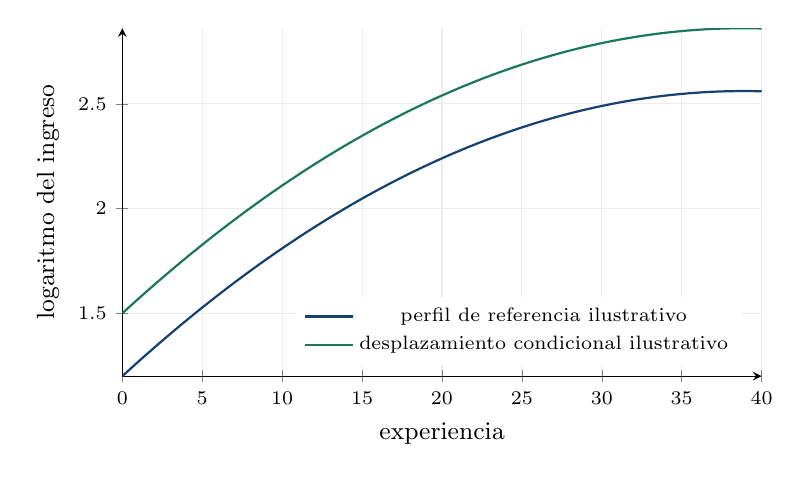
\begin{tikzpicture}
\begin{axis}[base,width=.8\textwidth,height=6cm,xmin=0,xmax=40,xlabel={experiencia},ylabel={logaritmo del ingreso},legend pos=south east]
\addplot[azul,thick,domain=0:40]{1.2+.07*x-.0009*x*x};
\addlegendentry{perfil de referencia ilustrativo}
\addplot[verde,thick,domain=0:40]{1.5+.07*x-.0009*x*x};
\addlegendentry{desplazamiento condicional ilustrativo}
\end{axis}
\end{tikzpicture}
\vfill
Archivo autónomo para la misma receta de LaTeX Workshop y MiKTeX.\\
Todas las tablas y figuras se incluyen en este único archivo.\\
Los laboratorios numéricos son artificiales; no sustituyen estimaciones de ENAHO.
\end{titlepage}
\tableofcontents
\clearpage
\phantomsection\addcontentsline{toc}{subsection}{La tesis y sus tres ecuaciones observables}
{\large\bfseries\color{azul}La tesis y sus tres ecuaciones observables}\par\vspace{2mm}
\section{La pregunta de la tesis y el significado del desarrollo matemático}

Este tratado acompaña la tesis de Estéfano Marcelo Ilizarbe Gonzales sobre TIC e ingresos de trabajadores formales e informales de Lima Metropolitana y Callao. Desarrolla las ecuaciones Mincer pooled y principal del archivo suministrado, junto con el apartado de Heckman proporcionado en el mensaje. Conserva sus regresores y sus letras. Los parámetros que se estiman son comunes a las personas de cada ecuación; el índice de persona identifica una fila, no un coeficiente diferente para cada persona.

La matemática distingue cuatro objetos: el ingreso horario observado, su logaritmo, la media condicional y el estimador calculado con una muestra. Por ejemplo,
\[
w_i=\ln(y_i),\qquad
w_i=\E[w_i\mid x_{i1},x_{i2},U_i,A_i,\operatorname{Informal}_i,y(i),m(i)]+\varepsilon_i.
\]
Una ecuación lineal especifica la media bajo una condición sobre el error. Una operación de mínimos cuadrados produce una proyección incluso si esa condición es falsa. La distinción reaparece en cada demostración de esperanza y covarianza.

Las tablas descriptivas de la tesis son información del documento, no microdatos disponibles para reestimar. Los laboratorios de este libro son artificiales, conservan todos los bloques de regresores y se identifican como tales. Ningún coeficiente de esos laboratorios se atribuye a la ENAHO.

La primera etapa de Heckman requiere otra muestra: personas de 14 a 65 años con información de selección y de sus regresores. La ecuación salarial necesita ingreso y horas válidas. Esta diferencia de muestras es parte del modelo, no un detalle de programación.

\clearpage
\section{Construcción del ingreso anual sin mezclar categorías de ocupación}

La tesis define el ingreso anual de la ocupación principal con dos variables de encuesta:
\[
\operatorname{IngresoAnual}_i=
\begin{cases}
\operatorname{I530A}_i,&\operatorname{P507}_i\in\{1,2\},\\
\operatorname{I524A1}_i,&\operatorname{P507}_i\in\{3,4,6\}.
\end{cases}
\]
El primer renglón representa empleadores e independientes; el segundo, empleados, obreros y trabajadores del hogar. No se suma ingreso de ambas fuentes para una misma persona. Una observación cuya categoría no satisface las reglas no recibe arbitrariamente cero.

La forma con indicadores reproduce las mismas condiciones:
\[
\begin{aligned}
\operatorname{IngresoAnual}_i={}&
\operatorname{I530A}_i\,\mathbf1\{\operatorname{P507}_i\in\{1,2\}\}\\
&+\operatorname{I524A1}_i\,\mathbf1\{\operatorname{P507}_i\in\{3,4,6\}\},
\end{aligned}
\]
pero esa igualdad se evalúa solamente donde la fuente correspondiente es válida. En software, un valor faltante no se convierte en una cantidad válida por multiplicarlo por cero.

Un independiente con ganancia anual S/ 31\,200 y un empleado con ingreso anual S/ 31\,200 tienen la misma magnitud anual en el ejercicio; no por ello sus conceptos contables originales son idénticos. La especificación salarial compara la transformación definida en la tesis, condicionando por sus controles productivos.

Las pruebas de sensibilidad con ingreso líquido y valores extremos cambian la variable dependiente o la muestra del ejercicio correspondiente. No se incorporan como nuevos controles en las tres ecuaciones.

\clearpage
\section{Del ingreso anual al ingreso horario y al logaritmo}

Si las horas semanales de la ocupación principal son positivas, la definición de la tesis es
\[
y_i=\operatorname{IngresoHora}_i=
\frac{\operatorname{IngresoAnual}_i}{52\,\operatorname{I513T}_i},
\qquad w_i=\ln(y_i).
\]
Usar propiedades del logaritmo da, paso por paso,
\[
\begin{aligned}
w_i
&=\ln\left(\frac{\operatorname{IngresoAnual}_i}{52\,\operatorname{I513T}_i}\right)\\
&=\ln(\operatorname{IngresoAnual}_i)-\ln(52\,\operatorname{I513T}_i)\\
&=\ln(\operatorname{IngresoAnual}_i)-\ln(52)-\ln(\operatorname{I513T}_i).
\end{aligned}
\]
Con ingreso anual 31\,200 y cuarenta horas semanales:
\[
y_i=\frac{31\,200}{52(40)}=15,\qquad w_i=\ln(15)=2.708050201.
\]
Las derivadas de la transformación, manteniendo fija la otra magnitud, son
\[
\frac{\partial w_i}{\partial\operatorname{IngresoAnual}_i}
=\frac1{\operatorname{IngresoAnual}_i},\qquad
\frac{\partial w_i}{\partial\operatorname{I513T}_i}
=-\frac1{\operatorname{I513T}_i}.
\]
El logaritmo no existe como número real si el ingreso horario es cero o negativo. Registrar a una persona sin ingreso válido con $w_i=0$ equivaldría a asignarle un ingreso horario de un sol. Esa operación alteraría el objeto dependiente y el mecanismo de selección.

\clearpage
\section{El ingreso y el año tienen papeles distintos en la notación}

Se conserva $w_i=\ln(y_i)$ para el logaritmo del ingreso horario. El símbolo $y(i)$ en $\lambda_{y(i)}$ identifica el año de entrevista de la persona. Por ello, $y_i$ es una cantidad monetaria positiva y $y(i)$ toma valores 2023, 2024 o 2025. Los paréntesis distinguen las dos funciones.
\[
\lambda_{y(i)}
=\lambda_{2023}\mathbf1\{y(i)=2023\}
+\lambda_{2024}\mathbf1\{y(i)=2024\}
+\lambda_{2025}\mathbf1\{y(i)=2025\}.
\]
Al adoptar 2023 como categoría base, la normalización es $\lambda_{2023}=0$. Análogamente, con enero como base,
\[
\mu_{m(i)}=\sum_{r=2}^{12}\mu_r\mathbf1\{m(i)=r\},\qquad \mu_1=0.
\]
Hay dos coeficientes de año y once de mes libres. Cada persona entra en un único año y un único mes. La suma de dummies de año y la suma de dummies de mes son ambas uno.

Los efectos temporales de la selección tienen su propia ecuación. Se escribe un superíndice $(S)$ cuando ambas ecuaciones aparecen juntas para evitar imponer que sus coeficientes sean iguales. El superíndice identifica parámetros de una ecuación ya solicitada; no añade regresores.

La razón de Mills $\widehat\lambda_i$ lleva índice de persona y sombrero. No es el efecto de año $\lambda_{y(i)}$. Ambos aparecen con todos sus argumentos cuando se multiplican o se derivan.

\clearpage
\section{Mincer pooled tal como está escrito en la tesis}

La ecuación de referencia es
\[
w_i=\alpha+x_{i1}^{\mathsf T}\gamma_1+x_{i2}^{\mathsf T}\gamma_2
+\lambda_{y(i)}+\mu_{m(i)}+\varepsilon_i. \tag{T9}
\]
Aquí $x_{i1}$ contiene educación, experiencia y experiencia al cuadrado. Es una columna de tres entradas:
\[
x_{i1}=
\begin{pmatrix}x_{i1,1}\\x_{i1,2}\\x_{i1,3}\end{pmatrix}
=\begin{pmatrix}
\text{Educación}_i\\
\operatorname{Experiencia}_i\\
(\operatorname{Experiencia}_i)^2
\end{pmatrix},\qquad
\gamma_1=\begin{pmatrix}\gamma_{1,1}\\\gamma_{1,2}\\\gamma_{1,3}\end{pmatrix}.
\]
La multiplicación se despliega:
\[
x_{i1}^{\mathsf T}\gamma_1
=\text{Educación}_i\gamma_{1,1}
+\operatorname{Experiencia}_i\gamma_{1,2}
+(\operatorname{Experiencia}_i)^2\gamma_{1,3}.
\]
El bloque $x_{i2}$ conserva género, estado civil, jefatura del hogar y efectos de sector y ocupación. Su dimensión depende de la codificación categórica efectivamente utilizada. No se inventan niveles de las categorías a partir de una ecuación que no los enumera.

El índice $i$ pertenece a los datos, mientras que $\gamma_1$ es el mismo vector de pendientes para todo el pool. Escribir $\gamma_{1i}$ implicaría pendientes individuales y requeriría otro modelo, que no se estima aquí.

\clearpage
\section{Desplegar todos los controles personales y productivos existentes}

Para exponer los productos se ordena $x_{i2}$ según el texto de la tesis. Sus primeras entradas son género, estado civil y jefatura. Si el estado civil se implementa mediante la dummy casado/a de las descriptivas, esas tres entradas son
\[
(x_{i2,1},x_{i2,2},x_{i2,3})
=(\operatorname{Mujer}_i,\operatorname{Casado}_i,\operatorname{Jefe}_i).
\]
Si el archivo de estimación utiliza varias categorías de estado civil, se conserva una entrada por cada categoría no base. La ecuación de la tesis no determina por sí sola cuántas de ellas hay.

Con las categorías productivas efectivas, la misma suma es
\[
\begin{aligned}
x_{i2}^{\mathsf T}\gamma_2={}&
\operatorname{Mujer}_i\gamma_{2,1}
+\operatorname{Casado}_i\gamma_{2,2}
+\operatorname{Jefe}_i\gamma_{2,3}\\
&+\sum_{\substack{s\text{ sector}\\s\ne s_0}}
\mathbf1\{\operatorname{Sector}_i=s\}\gamma_{2,s}^{(\mathrm{sector})}\\
&+\sum_{\substack{o\text{ ocupación}\\o\ne o_0}}
\mathbf1\{\text{Ocupación}_i=o\}\gamma_{2,o}^{(\text{ocupación})}.
\end{aligned}
\]
Los superíndices separan coeficientes del mismo bloque $\gamma_2$. No convierten sector u ocupación en variables adicionales. Cada suma recorre las categorías que ya conforman esos efectos fijos.

No se incluye tamaño del hogar, trabajador independiente ni Internet laboral solamente porque aparecen en tablas descriptivas. Un dato descriptivo y un regresor de las ecuaciones (9)--(12) cumplen funciones distintas.

\clearpage
\section{La ecuación principal literal conserva el conteo y la interacción centrada}

La ecuación (10) del archivo recibido se escribe literalmente como
\[
\begin{aligned}
w_i={}&\alpha+\beta_uU_i+\beta_aA_i+\theta\operatorname{Informal}_i\\
&+\delta_uU_i\operatorname{Informal}_i
+\delta_a\widetilde A_i\operatorname{Informal}_i\\
&+x_{i1}^{\mathsf T}\gamma_1+x_{i2}^{\mathsf T}\gamma_2
+\lambda_{y(i)}+\mu_{m(i)}+\varepsilon_i.
\end{aligned}\tag{T10}
\]
La variable $A_i$ es el conteo de actividades y $\widetilde A_i=U_i(A_i-\overline A_u)$. Se distinguen porque una aparece sin centrar en el efecto principal y la otra, centrada, en la interacción. Las operaciones de estimación de este tratado parten de esa escritura.

Para los no usuarios se usa el conteo total definido con cero; para los usuarios el conteo proviene de las nueve respuestas de actividades. Por tanto,
\[
U_i\in\{0,1\},\quad A_i\in\{0,\ldots,9\},\quad
U_i=0\Longrightarrow A_i=0,\quad U_iA_i=A_i.
\]
Estas identidades son necesarias para demostrar la equivalencia con una presentación que centra también el efecto principal. Un salto de cuestionario no se trata como una respuesta negativa entre usuarios.

Los cinco parámetros digitales y de informalidad se mantienen: $\beta_u,\beta_a,\theta,\delta_u,\delta_a$. Las columnas de educación, experiencia, controles y calendario permanecen completas.

\clearpage
\section{Por qué la interpretación de uso depende de cuál conteo aparece}

Considérese un formal y manténganse fijos los controles y el calendario. En la fórmula literal, comparar un usuario con $A_i=\overline A_u$ y un no usuario da
\[
\begin{aligned}
&[\alpha+\beta_u+\beta_a\overline A_u+x_{i1}^{\mathsf T}\gamma_1
+x_{i2}^{\mathsf T}\gamma_2+\lambda_{y(i)}+\mu_{m(i)}]\\
&\quad-[\alpha+x_{i1}^{\mathsf T}\gamma_1
+x_{i2}^{\mathsf T}\gamma_2+\lambda_{y(i)}+\mu_{m(i)}]\\
&=\beta_u+\overline A_u\beta_a.
\end{aligned}
\]
Con la referencia descriptiva 6.255, esa diferencia es $\beta_u+6.255\beta_a$. En la fórmula que contiene $\beta_a\widetilde A_i$ en lugar de $\beta_aA_i$, la misma comparación sí es $\beta_u$.

Para los informales en la fórmula literal, el contraste de uso a la media es
\[
\beta_u+\overline A_u\beta_a+\delta_u,
\]
porque $\widetilde A_i=0$ en un usuario situado exactamente en la media. El efecto intensivo entre usuarios es $\beta_a$ para formales y $\beta_a+\delta_a$ para informales en ambas presentaciones.

Las igualdades demuestran el detalle de notación encontrado en la tesis. No se corrige silenciosamente un símbolo para mantener una interpretación que la ecuación escrita no produce.

\clearpage
\section{Reparametrizar el centrado sin cambiar variables ni predicciones}

De $U_iA_i=A_i$ y $\widetilde A_i=U_i(A_i-\overline A_u)$ se deduce
\[
\widetilde A_i=A_i-\overline A_uU_i,\qquad
A_i=\widetilde A_i+\overline A_uU_i.
\]
Sustituir en el bloque digital literal produce
\[
\begin{aligned}
\beta_uU_i+\beta_aA_i
&=\beta_uU_i+\beta_a(\widetilde A_i+\overline A_uU_i)\\
&=(\beta_u+\overline A_u\beta_a)U_i+\beta_a\widetilde A_i.
\end{aligned}
\]
La presentación centrada asigna al coeficiente de $U_i$ el valor $\beta_u+\overline A_u\beta_a$ de la presentación literal. No son dos estimaciones contradictorias: son dos coordenadas de la misma superficie ajustada.
\[
\begin{pmatrix}\widehat\beta_u+\overline A_u\widehat\beta_a\\
\widehat\beta_a\end{pmatrix}
=\begin{pmatrix}1&\overline A_u\\0&1\end{pmatrix}
\begin{pmatrix}\widehat\beta_u\\\widehat\beta_a\end{pmatrix}.
\]
La matriz triangular tiene determinante uno y es invertible. El espacio generado por las dos columnas es el mismo. Para referencia fija, la covarianza se transforma multiplicando esa matriz a izquierda y su transpuesta a derecha.

Este libro muestra las dos coordenadas, identificándolas en cada comparación. Los símbolos nuevos de matrices auxiliares por fila no se utilizan.

\clearpage
\section{La media de actividades y lo que significa centrar entre usuarios}

El centrado se realiza usando la media entre quienes tienen $U_i=1$:
\[
\overline A_u=\frac{\sum_{i=1}^{n}U_iA_i}{\sum_{i=1}^{n}U_i}.
\]
Con $\sum_iU_i>0$,
\[
\begin{aligned}
\sum_{i=1}^{n}\widetilde A_i
&=\sum_iU_iA_i-\overline A_u\sum_iU_i\\
&=\sum_iU_iA_i-
\frac{\sum_iU_iA_i}{\sum_iU_i}\sum_iU_i=0.
\end{aligned}
\]
Por tanto, la media total de la variable centrada es cero en la misma muestra que define la referencia. El valor de 6.255 publicado está redondeado: usarlo en lugar de la media con todos sus decimales puede dejar una suma pequeña distinta de cero.

No se sigue que la media de $\widetilde A_i$ sea cero por año o por informalidad. Dentro del año 2023, por ejemplo,
\[
\frac{\sum_{y(i)=2023}\widetilde A_i}{n_{2023}}
=\frac{\sum_{y(i)=2023}U_i}{n_{2023}}
\left[
\frac{\sum_{y(i)=2023}U_iA_i}{\sum_{y(i)=2023}U_i}
-\overline A_u\right].
\]
Esta identidad explica por qué la tesis puede reportar una media anual negativa y una media total cero. El promedio anual depende tanto de la intensidad entre usuarios como de su proporción.

\clearpage
\section{Qué conserva el pooled y qué requiere una hipótesis adicional}

Agrupar los cortes de 2023, 2024 y 2025 apila filas. Para la ecuación principal:
\[
\begin{pmatrix}w^{(2023)}\\w^{(2024)}\\w^{(2025)}\end{pmatrix}
=
\begin{pmatrix}W^{(2023)}\\W^{(2024)}\\W^{(2025)}\end{pmatrix}\beta
+\begin{pmatrix}\varepsilon^{(2023)}\\\varepsilon^{(2024)}\\\varepsilon^{(2025)}\end{pmatrix}.
\]
Las matrices $W^{(y)}$ contienen los regresores ya definidos y las dummies temporales correspondientes. El vector $\beta$ reúne sus coeficientes, como se hará también en la ecuación salarial de Heckman. No reemplaza a $\beta_u$ o $\beta_a$; muestra dónde están dentro del vector.

Pooled impone pendientes comunes, por ejemplo una sola $\beta_a$ para los tres años. Las dummies de año permiten diferentes interceptos, no diferentes pendientes digitales. Para afirmar que la pendiente poblacional es común se necesita una hipótesis económica y estadística adicional; el mero apilamiento no la demuestra.

Tampoco se deduce independencia entre personas por llamarlo pooled. Personas del mismo hogar o conglomerado pueden compartir shocks. Las matrices de covarianza se desarrollan tanto para independencia entre filas como para dependencia dentro de los grupos existentes.

No se agregan interacciones por año a la especificación principal. Cuando se examina qué significaría una pendiente distinta se presenta como una limitación de la hipótesis, no como un cuarto modelo estimado.

\clearpage
\section{Las cifras de la tesis delimitan la muestra y no determinan los coeficientes}

El documento reporta 18\,065 personas en la muestra final y 7\,933 usuarios. Las cantidades anuales 6\,090, 6\,004 y 5\,971 suman
\[
6\,090+6\,004+5\,971=18\,065.
\]
Los formales 7\,850 y los informales 10\,215 también suman 18\,065. Son controles de consistencia del archivo.

Una tabla de medias no determina $\widehat\beta_a$. Para estimar MCO se necesitan productos cruzados de todos los regresores con cada otro regresor y con $w_i$:
\[
\sum_i W_{ij}W_{ik},\qquad \sum_iW_{ij}w_i.
\]
Conocer solamente $\sum_iW_{ij}/n$ no permite recuperar, por ejemplo,
$\sum_i A_i\,\text{Educación}_i$ o
$\sum_iU_i\,\operatorname{Informal}_i\,w_i$. Dos muestras pueden compartir todas las medias univariadas y tener covarianzas distintas.

Los promedios de ingreso formal e informal tampoco equivalen a $\theta$. En la ecuación principal, la diferencia incluye composición educativa, productiva, digital y temporal.

Se conserva la muestra documentada en los comentarios aplicados, pero no se inventa una base de selección de 18\,065 personas. La base salarial ya excluyó ingresos y horas inválidas y puede excluir no ocupados; no es automáticamente el universo del probit.

\clearpage
\section{Heckman pooled conserva la ecuación de selección propuesta}

El apartado facilitado propone
\[
S_i^*=Z_i^{\mathsf T}\pi+\lambda_{y(i)}+\mu_{m(i)}+\nu_i,
\qquad S_i=\mathbf1\{S_i^*>0\}. \tag{T11}
\]
Al considerar simultáneamente las dos ecuaciones se escribe
\[
Z_i^{\mathsf T}\pi+\lambda_{y(i)}^{(S)}+\mu_{m(i)}^{(S)}
=\sum_{l=1}^{p_Z}Z_{il}\pi_l
+\sum_{a=2024}^{2025}\lambda_a^{(S)}\mathbf1\{y(i)=a\}
+\sum_{r=2}^{12}\mu_r^{(S)}\mathbf1\{m(i)=r\}.
\]
El intercepto, si está en $Z_i$, tiene una entrada igual a uno. No se añade un segundo intercepto además de esa entrada. La varianza de $\nu_i$ se fija en uno para identificar la escala del probit.

El texto no enumera todo el contenido de $Z_i$. Por eso no se declara como definitiva una lista de primera etapa inventada. Los desarrollos de cada $\pi_l$ valen para los regresores de $Z_i$ que finalmente se justifiquen y estén disponibles para $S_i=0$ y $S_i=1$.

Las dos exclusiones tentativas sí están identificadas: menores de seis años e ingreso no laboral del hogar. Se desarrollan su relevancia, la restricción de media de resultado y la sensibilidad a una violación.

\clearpage
\section{La ecuación salarial corregida y el despliegue de su vector}

La propuesta de segunda etapa es
\[
\ln(y_i)=W_i^{\mathsf T}\beta+\kappa\widehat\lambda_i+\varepsilon_i,
\qquad S_i=1. \tag{T12}
\]
En el desarrollo de la ecuación principal, el vector $W_i$ conserva, en este orden,
\[
\begin{aligned}
W_i^{\mathsf T}={}&\Bigl(
1,U_i,A_i,\operatorname{Informal}_i,
U_i\operatorname{Informal}_i,\widetilde A_i\operatorname{Informal}_i,\\
&
x_{i1}^{\mathsf T},x_{i2}^{\mathsf T},
\mathbf1\{y(i)=2024\},\mathbf1\{y(i)=2025\},
(\mathbf1\{m(i)=r\})_{r=2}^{12}
\Bigr).
\end{aligned}
\]
El vector de coeficientes sigue exactamente ese orden:
\[
\beta^{\mathsf T}=
\left(
\alpha,\beta_u,\beta_a,\theta,\delta_u,\delta_a,
\gamma_1^{\mathsf T},\gamma_2^{\mathsf T},
\lambda_{2024},\lambda_{2025},(\mu_r)_{r=2}^{12}
\right).
\]
Cuando se corrige la Mincer de referencia se utilizan las mismas entradas salvo las cinco columnas digitales y de informalidad ausentes en (T9). No se obtiene otro modelo con controles escogidos para simplificar una demostración.

La palabra $\varepsilon_i$ en (T12) designa el error de media cero después de corregir selección. Más adelante se escribe la diferencia entre ese error y el error salarial original mediante una igualdad, para no imponerles simultáneamente dos medias incompatibles.

\clearpage
\section{La selección no convierte el ingreso ausente en ingreso cero}

El indicador definido en el mensaje vale uno cuando el ingreso laboral horario es observable y válido. Es posible ser ocupado y tener $S_i=0$ por falta de ingreso u horas válidas. Por eso, el evento no es necesariamente idéntico a participación laboral.
\[
S_i=1\Longrightarrow y_i>0,\quad \operatorname{I513T}_i>0,
\quad\text{y las fuentes necesarias son observables}.
\]
La observación estadística de Heckman es $(S_i,Z_i,W_i,w_i\text{ si }S_i=1)$, con los requisitos de disponibilidad que correspondan. Para $S_i=0$ la contribución salarial no se evalúa sustituyendo $w_i=0$.
\[
\Prob(S_i=0\mid Z_i,y(i),m(i))
=1-\Phi\left(\sum_lZ_{il}\pi_l+\lambda_{y(i)}^{(S)}+\mu_{m(i)}^{(S)}\right).
\]
La densidad conjunta para $S_i=1$ sí incorpora $w_i$. Se deriva a partir de una normal bivariada de los dos errores, no de una regla de censura del ingreso en cero.

Si $S_i=0$ reúne no ocupación, no respuesta y horas inválidas, una sola normal de selección es una hipótesis sobre esa observabilidad compuesta. Se puede estudiar su sensibilidad sin afirmar que una dummy de empleo representa exactamente todos esos mecanismos.

\clearpage
\section{Disponibilidad de informalidad, sector y ocupación en la población de selección}

Informalidad, sector y ocupación describen un puesto. Para una persona sin puesto observado, puede faltar su valor. No existe una regla matemática que permita convertir esos faltantes en empleo formal o en el sector base.

La primera etapa solamente exige el contenido de $Z_i$ y el calendario. Si $Z_i$ incluyera una característica laboral no definida para $S_i=0$, el probit terminaría nuevamente condicionado a quienes la reportan. Esta eliminación puede impedir representar el evento planteado.

En dos etapas, la ecuación de resultado utiliza $W_i$ únicamente para $S_i=1$. La densidad marginal de $S_i=0$ de un Heckman condicional no contiene directamente $W_i$. Sin embargo, interpretar una ecuación de salario potencial para todos exige que sus características productivas potenciales tengan un significado económico.

Mantener los controles existentes no autoriza a afirmar que se identificaron puestos contrafactuales de todos los no ocupados. Se separan el procedimiento algebraico de estimación y el alcance de la interpretación.
\[
\E[w_i\mid W_i,Z_i,S_i=1]
=W_i^{\mathsf T}\beta+\rho\sigma
\frac{\phi(Z_i^{\mathsf T}\pi+\lambda_{y(i)}^{(S)}+\mu_{m(i)}^{(S)})}
{\Phi(Z_i^{\mathsf T}\pi+\lambda_{y(i)}^{(S)}+\mu_{m(i)}^{(S)})}.
\]
La igualdad exige que los condicionantes usados en ella estén definidos. No es una receta para rellenar con ceros cualquier dato de puesto ausente.

\clearpage
\section{Las condiciones que cada demostración hará visibles}

MCO tiene una expresión algebraica bajo rango completo; su insesgadez requiere media cero del error condicional al diseño. Una covarianza homocedástica exige además igual varianza y ausencia de correlación entre filas. La matriz robusta relaja igualdad de varianzas; no demuestra media cero.

Heckman normal impone una distribución conjunta:
\[
\begin{pmatrix}\varepsilon_i^{(0)}\\\nu_i\end{pmatrix}
\Bigm|W_i,Z_i,y(i),m(i)
\sim N_2\left[
\begin{pmatrix}0\\0\end{pmatrix},
\begin{pmatrix}\sigma^2&\rho\sigma\\\rho\sigma&1\end{pmatrix}\right],
\quad \sigma>0,\ |\rho|<1.
\]
El superíndice $(0)$ identifica el error salarial antes de restar su media seleccionada. No es una nueva variable explicativa.

Las derivadas, integrales y resultados asintóticos se explican bajo esas condiciones. Cuando solo existe una proyección estadística, se indica que sus coeficientes describen asociaciones. La corrección de selección no elimina por definición la simultaneidad entre ingreso y uso de TIC.

El modelo se mantiene constante durante el desarrollo. Las transformaciones del conteo o de la escala numérica se demuestran como cambios invertibles de coordenadas y se reconstruyen en las unidades de la tesis. Las pruebas de sensibilidad expresamente previstas en el documento se presentan después de la estimación principal.

\clearpage
\phantomsection\addcontentsline{toc}{subsection}{Probabilidad, momentos y cálculo de vectores desde sus definiciones}
{\large\bfseries\color{azul}Probabilidad, momentos y cálculo de vectores desde sus definiciones}\par\vspace{2mm}
\section{Variable aleatoria, realización y condicionamiento en las tres ecuaciones}

Una variable aleatoria asigna un número a cada resultado posible del mecanismo de muestreo. $w_i$ representa un logaritmo de ingreso que podría cambiar con la muestra; su realización observada es el número utilizado en una fila. Condicionar al diseño significa mantener fijas todas las columnas que lo componen y dejar variar los errores.
\[
\E[w_i\mid W]=\int_{\mathbb R}t\,f_{w_i\mid W}(t)\,\mathrm dt,
\quad
\Var(w_i\mid W)=\int_{\mathbb R}
(t-\E[w_i\mid W])^2f_{w_i\mid W}(t)\,\mathrm dt.
\]
La integral requiere que exista el momento correspondiente. En la ecuación lineal $w_i=W_i^{\mathsf T}\beta+\varepsilon_i$,
\[
\E[w_i\mid W]=W_i^{\mathsf T}\beta+\E[\varepsilon_i\mid W].
\]
Para identificar la media con la combinación de regresores se impone $\E[\varepsilon_i\mid W]=0$. Para una sola fila, $\E[\varepsilon_i]=0$ no basta: una relación sistemática entre educación y error puede desaparecer al promediar personas y seguir afectando la pendiente.

La condición usada para una esperanza exacta de MCO se refiere a todo el diseño, no solo a la columna del coeficiente que interesa. En Heckman se condiciona además al evento de selección; ese evento puede cambiar la media del error aun cuando la media antes de seleccionarlo sea cero.

\clearpage
\section{Linealidad de la esperanza y por qué no requiere independencia}

Para constantes $c_j$ y variables con primer momento finito,
\[
\begin{aligned}
\E\left[\sum_{j=1}^{p}c_jw_j\right]
&=\int\cdots\int\left(\sum_jc_jt_j\right)
f_{w_1,\ldots,w_p}(t_1,\ldots,t_p)\,\mathrm dt_1\cdots\mathrm dt_p\\
&=\sum_jc_j\int\cdots\int t_j
f_{w_1,\ldots,w_p}(t_1,\ldots,t_p)\,\mathrm dt_1\cdots\mathrm dt_p\\
&=\sum_jc_j\E[w_j].
\end{aligned}
\]
Integrar las otras coordenadas produce la densidad marginal de $w_j$. No se factoriza una densidad conjunta en el argumento.

Condicionalmente, si $W_{ij}$ es conocido al fijar el diseño,
\[
\E\left[\sum_iW_{ij}\varepsilon_i\mid W\right]
=\sum_iW_{ij}\E[\varepsilon_i\mid W].
\]
El paso permite deducir insesgadez sin exigir normalidad. En cambio, si $W_{ij}$ incluye una razón de Mills estimada con los mismos datos, no se trata como constante frente a la aleatoriedad completa de la primera etapa.

Ejemplo: $\varepsilon_1=\varepsilon_2$ con media cero. La suma tiene media cero aun con dependencia perfecta. Su varianza es cuatro veces la varianza individual. Esperanza y varianza utilizan propiedades distintas.

\clearpage
\section{Varianza y covarianza escalares: abrir los cuadrados}

Con segundos momentos finitos,
\[
\begin{aligned}
\Var(w_i)&=\E[(w_i-\E[w_i])^2]\\
&=\E[w_i^2]-2\E[w_i]\E[w_i]+(\E[w_i])^2\\
&=\E[w_i^2]-(\E[w_i])^2,\\
\Cov(w_i,w_k)&=\E[(w_i-\E[w_i])(w_k-\E[w_k])]\\
&=\E[w_iw_k]-\E[w_i]\E[w_k].
\end{aligned}
\]
Para dos constantes $c_1,c_2$:
\[
\Var(c_1w_i+c_2w_k)
=c_1^2\Var(w_i)+c_2^2\Var(w_k)+2c_1c_2\Cov(w_i,w_k).
\]
La demostración consiste en expandir el cuadrado del error centrado y aplicar linealidad. La covarianza no se omite por el hecho de que las variables tengan nombres distintos.

En la asociación intensiva informal se aplica directamente:
\[
\Var(\widehat\beta_a+\widehat\delta_a)
=\Var(\widehat\beta_a)+\Var(\widehat\delta_a)
+2\Cov(\widehat\beta_a,\widehat\delta_a).
\]
Si las varianzas son .0004 y .0009 y la covarianza es -.0003, la varianza de la suma es .0007, no .0013. La matriz con esas entradas es positiva definida porque su determinante es $.0004(.0009)-(.0003)^2>0$.

\clearpage
\section{Cauchy Schwarz y los límites de una covarianza}

La no negatividad de un cuadrado impone, para todo número real $t$,
\[
0\le \E[(\varepsilon_i-t\varepsilon_k)^2]
=\Var(\varepsilon_i)-2t\Cov(\varepsilon_i,\varepsilon_k)
+t^2\Var(\varepsilon_k)
\]
cuando los errores tienen media cero. Si $\Var(\varepsilon_k)>0$, completar el cuadrado da
\[
0\le
\Var(\varepsilon_i)-
\frac{\Cov(\varepsilon_i,\varepsilon_k)^2}{\Var(\varepsilon_k)}.
\]
Se obtiene
\[
\abs{\Cov(\varepsilon_i,\varepsilon_k)}
\le\sqrt{\Var(\varepsilon_i)\Var(\varepsilon_k)}.
\]
La correlación divide la covarianza entre ese producto de desviaciones. Por tanto, está entre menos uno y uno. En Heckman, $\Cov(\varepsilon_i^{(0)},\nu_i)=\rho\sigma$ y la cota es $\abs{\rho}\le1$.

La matriz bivariada es no singular cuando $\sigma>0$ y $\abs{\rho}<1$. Su determinante es $\sigma^2(1-\rho^2)$. En el límite $\abs{\rho}=1$ un error queda determinado por el otro y la densidad bivariada ordinaria deja de existir.

\clearpage
\section{Esperanza iterada y partición entre seleccionados y no seleccionados}

Para una variable integrable y una información $Z_i$,
\[
\E[\varepsilon_i^{(0)}]
=\E[\E[\varepsilon_i^{(0)}\mid Z_i,S_i]].
\]
Al fijar $Z_i$ y particionar por un indicador binario:
\[
\begin{aligned}
\E[\varepsilon_i^{(0)}\mid Z_i]
={}&\Prob(S_i=1\mid Z_i)
\E[\varepsilon_i^{(0)}\mid Z_i,S_i=1]\\
&+\Prob(S_i=0\mid Z_i)
\E[\varepsilon_i^{(0)}\mid Z_i,S_i=0].
\end{aligned}
\]
Que la suma ponderada sea cero no impone cero a cada término. En selección normal, las dos medias tienen signos opuestos si $\rho\ne0$ y se compensan con sus probabilidades.

La identidad se prueba multiplicando cada densidad condicional por su probabilidad. Así se reconstruye la densidad original:
\[
f_{\varepsilon\mid Z}
=f_{\varepsilon\mid Z,S=1}\Prob(S=1\mid Z)
+f_{\varepsilon\mid Z,S=0}\Prob(S=0\mid Z).
\]
Integrar la variable multiplicada por ambos lados produce la esperanza. El mecanismo da la justificación probabilística de corregir una media seleccionada que puede no ser cero.

\clearpage
\section{La varianza total incluye dispersión dentro y entre condiciones}

Restar y sumar $\E[w_i\mid Z_i]$:
\[
w_i-\E[w_i]
=[w_i-\E[w_i\mid Z_i]]
+[\E[w_i\mid Z_i]-\E[w_i]].
\]
El cuadrado tiene dos cuadrados y un producto cruzado. La esperanza del producto es cero:
\[
\E\!\left[(w_i-\E[w_i\mid Z_i])
(\E[w_i\mid Z_i]-\E[w_i])\right]
=\E[(\E[w_i\mid Z_i]-\E[w_i])\,0]=0.
\]
Resulta
\[
\Var(w_i)=\E[\Var(w_i\mid Z_i)]
+\Var(\E[w_i\mid Z_i]).
\]
La fórmula condicional al resto de regresores se obtiene repitiendo la misma descomposición con esperanzas condicionales.

En una muestra dividida por informalidad, la varianza total de logaritmos de ingreso incluye varianzas dentro de cada grupo y la dispersión entre sus medias. Una diferencia descriptiva entre formales e informales no identifica por sí sola $\theta$, porque las medias también cambian con los otros regresores.

\clearpage
\section{Vectores de errores y matrices de covarianza desde las entradas}

Para $\varepsilon=(\varepsilon_1,\ldots,\varepsilon_n)^{\mathsf T}$, se define
\[
\Cov(\varepsilon\mid W)=
\E[(\varepsilon-\E[\varepsilon\mid W])
(\varepsilon-\E[\varepsilon\mid W])^{\mathsf T}\mid W].
\]
La entrada $(i,k)$ es $\Cov(\varepsilon_i,\varepsilon_k\mid W)$. La diagonal contiene $\Var(\varepsilon_i\mid W)$. La matriz es simétrica porque la multiplicación de escalares conmuta.

Para cualquier columna $c$:
\[
c^{\mathsf T}\Cov(\varepsilon\mid W)c
=\E\left[\left(\sum_i c_i
(\varepsilon_i-\E[\varepsilon_i\mid W])\right)^2\Bigm|W\right]\ge0.
\]
Esta desigualdad define semidefinición positiva. No afirma que todas las entradas sean positivas: una covarianza fuera de la diagonal puede ser negativa.

Si los errores son independientes condicionalmente, las covarianzas fuera de diagonal son cero. Si también tienen varianza común $\sigma^2$, la matriz es $\sigma^2I_n$. Heterocedasticidad conserva una diagonal con entradas distintas; dependencia por hogar produce bloques con covarianzas fuera de diagonal.

\clearpage
\section{Propagación lineal de todas las covarianzas con dobles sumas}

Para una matriz constante $C$ y un vector de errores con media cero, la coordenada $j$ de $C\varepsilon$ es $\sum_iC_{ji}\varepsilon_i$. Por ello:
\[
\begin{aligned}
\Cov((C\varepsilon)_j,(C\varepsilon)_k\mid W)
&=\E\left[\sum_iC_{ji}\varepsilon_i
\sum_lC_{kl}\varepsilon_l\Bigm|W\right]\\
&=\sum_i\sum_lC_{ji}C_{kl}
\Cov(\varepsilon_i,\varepsilon_l\mid W).
\end{aligned}
\]
Reunir las entradas da
\[
\Cov(C\varepsilon\mid W)=C\Cov(\varepsilon\mid W)C^{\mathsf T}.
\]
La igualdad vale con dependencia entre filas. Si solo existe diagonal, se reduce a
\[
\sum_iC_{ji}C_{ki}\Var(\varepsilon_i\mid W).
\]
En MCO, $C$ será la matriz concreta
$[\sum_iW_iW_i^{\mathsf T}]^{-1}(W_1,\ldots,W_n)$.
Esta escritura exhibe los productos cruzados y la relación entre las observaciones y cada coeficiente. En los laboratorios se reconstruyen sus filas y se comprueba numéricamente la misma igualdad.

\clearpage
\section{Productos internos, productos exteriores y las dimensiones que se multiplican}

Una columna $W_i\in\mathbb R^p$ y otra columna $\beta\in\mathbb R^p$ producen un escalar:
\[
W_i^{\mathsf T}\beta=\sum_{j=1}^{p}W_{ij}\beta_j.
\]
El producto en orden contrario, $W_iW_i^{\mathsf T}$, es una matriz de dimensión $p\times p$:
\[
W_iW_i^{\mathsf T}
=\begin{pmatrix}
W_{i1}^2&W_{i1}W_{i2}&\cdots&W_{i1}W_{ip}\\
W_{i2}W_{i1}&W_{i2}^2&\cdots&W_{i2}W_{ip}\\
\vdots&\vdots&\ddots&\vdots\\
W_{ip}W_{i1}&W_{ip}W_{i2}&\cdots&W_{ip}^2
\end{pmatrix}.
\]
Con $\varepsilon_i$ escalar, $W_i\varepsilon_i$ es una columna, no una matriz cuadrada. El producto $W_iW_i^{\mathsf T}\varepsilon_i^2$ tiene la dimensión de una matriz de covarianza de momentos.

En la ecuación principal, las entradas iniciales son $1,U_i,A_i,\operatorname{Informal}_i,U_i\operatorname{Informal}_i,\widetilde A_i\operatorname{Informal}_i$. Por ejemplo, la entrada $(3,5)$ del producto exterior es $A_iU_i\operatorname{Informal}_i$. La identidad $A_iU_i=A_i$ simplifica ese producto, pero no elimina ninguno de sus parámetros.

\clearpage
\section{La matriz de productos cruzados se demuestra mediante sus coordenadas}

Al apilar las filas $W_i^{\mathsf T}$ en $W$, la entrada $(j,k)$ de $W^{\mathsf T}W$ es
\[
(W^{\mathsf T}W)_{jk}=
\sum_{i=1}^{n}(W^{\mathsf T})_{ji}W_{ik}
=\sum_iW_{ij}W_{ik}.
\]
Por lo tanto,
\[
W^{\mathsf T}W=
\begin{pmatrix}
\sum_iW_{i1}^2&\sum_iW_{i1}W_{i2}&\cdots&\sum_iW_{i1}W_{ip}\\
\sum_iW_{i2}W_{i1}&\sum_iW_{i2}^2&\cdots&\sum_iW_{i2}W_{ip}\\
\vdots&\vdots&\ddots&\vdots\\
\sum_iW_{ip}W_{i1}&\sum_iW_{ip}W_{i2}&\cdots&\sum_iW_{ip}^2
\end{pmatrix}.
\]
No se rebautiza esta matriz como una letra para esconder sus sumas. Cada uso de la inversa puede leerse como la solución de este sistema completo.

La simetría surge de $W_{ij}W_{ik}=W_{ik}W_{ij}$. Para una columna $c$:
\[
c^{\mathsf T}\left[\sum_iW_iW_i^{\mathsf T}\right]c
=\sum_i(W_i^{\mathsf T}c)^2.
\]
La matriz es positiva definida exactamente cuando ninguna combinación lineal no nula de sus columnas produce cero en todas las filas. Esa es la condición de rango completo utilizada para estimar los coeficientes.

\clearpage
\section{Rango, invertibilidad y singularidad por dummies completas}

Si existe una columna $c\ne0$ con $Wc=0$, entonces
\[
\left[\sum_iW_iW_i^{\mathsf T}\right]c=W^{\mathsf T}Wc=0.
\]
La matriz tiene un vector no nulo en su núcleo y no puede tener inversa. En sentido contrario, si el producto cruzado es singular, un $c\ne0$ satisface
$c^{\mathsf T}W^{\mathsf T}Wc=0$; como es una suma de cuadrados, cada fila de $Wc$ es cero.

Con intercepto y todas las dummies de año:
\[
1-\mathbf1\{y(i)=2023\}
-\mathbf1\{y(i)=2024\}
-\mathbf1\{y(i)=2025\}=0\quad\text{para cada }i.
\]
La relación impide identificar cuatro interceptos independientes. Fijar $\lambda_{2023}=0$ elige una representación única de tres interceptos anuales.

Lo mismo ocurre con doce dummies mensuales y con todas las categorías de sector y ocupación. Omitir una categoría por bloque es una normalización; no implica que las personas de esa categoría desaparezcan de la muestra ni que tengan ingreso cero.

Rango puede fallar aun con esas bases elegidas, por ejemplo si cada sector solo aparece en un año. Hay que verificar la matriz conjunta, no únicamente cada bloque por separado.

\clearpage
\section{Gradiente de un escalar respecto de una columna de parámetros}

Si $w_i-W_i^{\mathsf T}\beta=w_i-\sum_jW_{ij}\beta_j$, el residuo tiene derivada
\[
\frac{\partial(w_i-\sum_lW_{il}\beta_l)}{\partial\beta_j}
=-W_{ij}.
\]
La regla de cadena para su cuadrado produce
\[
\frac{\partial(w_i-\sum_lW_{il}\beta_l)^2}{\partial\beta_j}
=-2W_{ij}(w_i-\sum_lW_{il}\beta_l).
\]
El gradiente apila estas derivadas en una columna de $p$ entradas. Diferenciar de nuevo respecto de $\beta_k$ da
\[
\frac{\partial^2(w_i-\sum_lW_{il}\beta_l)^2}
{\partial\beta_j\partial\beta_k}=2W_{ij}W_{ik}.
\]
La Hessiana reúne esos productos y es simétrica. La demostración usa que los regresores se mantienen fijos al derivar los parámetros. Cuando una columna depende de un parámetro estimado en primera etapa, se aplica además la derivada de esa columna.

En el coeficiente $\delta_a$, $W_{ij}=\widetilde A_i\operatorname{Informal}_i$. Por ello el gradiente correspondiente multiplica el residuo por ese producto completo, no solamente por $\widetilde A_i$.

\clearpage
\section{Diferencial de una matriz inversa y su aplicación a los estimadores}

Sea un producto cruzado invertible $W^{\mathsf T}W$ que cambia con una perturbación del diseño. Diferenciar la identidad
\[
(W^{\mathsf T}W)^{-1}(W^{\mathsf T}W)=I_p
\]
da
\[
\mathrm d[(W^{\mathsf T}W)^{-1}](W^{\mathsf T}W)
+(W^{\mathsf T}W)^{-1}\mathrm d(W^{\mathsf T}W)=0.
\]
Multiplicar a derecha por la inversa despeja
\[
\mathrm d[(W^{\mathsf T}W)^{-1}]
=-(W^{\mathsf T}W)^{-1}
\mathrm d(W^{\mathsf T}W)(W^{\mathsf T}W)^{-1}.
\]
Además,
\[
\mathrm d(W^{\mathsf T}W)
=(\mathrm dW)^{\mathsf T}W+W^{\mathsf T}(\mathrm dW).
\]
En Heckman cambia la última columna de la matriz ampliada porque cambia la razón estimada. La fórmula muestra que el cambio del estimador proviene tanto del producto con el resultado como de la inversa del producto cruzado.

Las matrices deben permanecer en el orden mostrado; en general, dos matrices no conmutan. La regla escalar para $1/t$ es un caso de dimensión uno, no una licencia para intercambiar factores matriciales.

\clearpage
\section{Taylor vectorial con resto y la base de las aproximaciones de inferencia}

Para una función escalar diferenciable $g$ de los parámetros $\beta$, tomar el segmento $\beta+t h$ y aplicar el teorema fundamental del cálculo:
\[
g(\beta+h)-g(\beta)
=\int_0^1\nabla g(\beta+t h)^{\mathsf T}h\,\mathrm dt.
\]
Restar $\nabla g(\beta)^{\mathsf T}h$:
\[
g(\beta+h)-g(\beta)-\nabla g(\beta)^{\mathsf T}h
=\int_0^1[\nabla g(\beta+t h)-\nabla g(\beta)]^{\mathsf T}h\,\mathrm dt.
\]
Si la Hessiana es continua, una segunda integración da un resto de orden $\norm h^2$:
\[
\int_0^1(1-t)\,h^{\mathsf T}
\nabla^2g(\beta+t h)h\,\mathrm dt.
\]
Al usar $h=\widehat\beta-\beta$, la aproximación solo desprecia ese resto cuando la consistencia y las tasas justifican que sea pequeño.

Para $g(\beta)=100(e^{\beta_a+\delta_a}-1)$, el gradiente tiene dos entradas no nulas, ambas $100e^{\beta_a+\delta_a}$. La covarianza de los dos coeficientes entra necesariamente en el error estándar de la diferencia porcentual.

\clearpage
\section{Ley de grandes números y teorema central para los momentos del modelo}

Para observaciones independientes con momentos suficientes,
\[
\frac1n\sum_iW_iW_i^{\mathsf T}
\xrightarrow{p}\E[W_iW_i^{\mathsf T}],\qquad
\frac1n\sum_iW_i\varepsilon_i\xrightarrow{p}0.
\]
Si el límite del producto cruzado es invertible, la continuidad de la inversa permite deducir consistencia. Una esperanza de media cero aislada no basta si el promedio no converge.

Con segundos momentos y condiciones del teorema central:
\[
\frac1{\sqrt n}\sum_iW_i\varepsilon_i
\xrightarrow{d}N_p\left(0,\E[W_iW_i^{\mathsf T}\varepsilon_i^2]\right).
\]
Insertar este límite en la identidad del estimador produce la normal asintótica de MCO. Las distribuciones anuales pueden ser distintas: un pooled con proporciones anuales estables conduce a promedios ponderados de sus momentos. No necesita declarar idénticas las medias anuales.

Con dependencia por conglomerado el objeto independiente es la suma de momentos dentro de cada conglomerado. La raíz relevante y las condiciones de máximo tamaño de grupo deben formularse sobre ese esquema.

Se distinguen resultados finitos exactos de resultados de gran muestra: una aproximación normal no demuestra que el estimador sea exactamente normal en una muestra heterocedástica.

\clearpage
\section{Bernoulli de selección y sus primeros dos momentos}

Al fijar sus regresores, $S_i$ tiene probabilidades $p_i$ y $1-p_i$ en uno y cero. Aquí se escribe la probabilidad entera:
\[
\Prob(S_i=1\mid Z_i,y(i),m(i))
=\Phi(Z_i^{\mathsf T}\pi+\lambda_{y(i)}^{(S)}+\mu_{m(i)}^{(S)}).
\]
Para la variable binaria:
\[
\E[S_i\mid Z_i]=1\Prob(S_i=1\mid Z_i)+0\Prob(S_i=0\mid Z_i),
\quad S_i^2=S_i.
\]
Así, la varianza es
\[
\begin{aligned}
\Var(S_i\mid Z_i,y(i),m(i))
={}&\Phi(Z_i^{\mathsf T}\pi+\lambda_{y(i)}^{(S)}+\mu_{m(i)}^{(S)})\\
&\times[1-\Phi(Z_i^{\mathsf T}\pi+\lambda_{y(i)}^{(S)}+\mu_{m(i)}^{(S)})].
\end{aligned}
\]
El máximo es $1/4$ cuando la probabilidad es $1/2$; en cero o uno la varianza se anula. En probit, las probabilidades se aproximan a esas fronteras sin alcanzarlas para argumentos finitos.

Un ajuste lineal de $S_i$ no reproduce automáticamente esa función de varianza ni garantiza probabilidades en el intervalo unitario. El vínculo normal se deriva posteriormente a partir del error $\nu_i$ y la regla de umbral.

\clearpage
\section{Normal, chi cuadrado, Student y F en las pruebas exactas de MCO}

Con errores $N_n(0,\sigma^2I_n)$ y diseño de rango $p$, una combinación lineal de errores es normal. El residuo de MCO proyecta esos errores sobre un subespacio de dimensión $n-p$.

Una base ortonormal en ese subespacio produce $n-p$ normales estándar independientes. La suma de sus cuadrados es, por definición, chi cuadrado:
\[
\frac{\sum_i\widehat\varepsilon_i^2}{\sigma^2}
\sim\chi^2_{n-p},\qquad
\E\left[\frac{\sum_i\widehat\varepsilon_i^2}{\sigma^2}\right]=n-p.
\]
Las proyecciones sobre subespacios ortogonales de una normal son independientes. Por eso:
\[
\frac{\widehat\beta_j-\beta_j}
{\sqrt{\widehat\sigma^2[(\sum_iW_iW_i^{\mathsf T})^{-1}]_{jj}}}
\sim t_{n-p},\quad
\widehat\sigma^2=\frac{\sum_i\widehat\varepsilon_i^2}{n-p}.
\]
La razón de dos chi cuadrados independientes, cada uno dividido por sus grados de libertad, define una distribución $F$. Se utiliza para restricciones lineales bajo homocedasticidad y normalidad.

Con covarianza robusta la justificación habitual es asintótica. No se proclama una distribución exacta $t_{n-p}$ por cambiar el denominador a un error estándar robusto.

\clearpage
\phantomsection\addcontentsline{toc}{subsection}{Mincer pooled y mínimos cuadrados con todos los controles}
{\large\bfseries\color{azul}Mincer pooled y mínimos cuadrados con todos los controles}\par\vspace{2mm}
\section{La matriz Mincer completa y el orden de sus coeficientes}

Para (T9), se apilan las filas sin eliminar controles:
\[
\begin{aligned}
(W_i^{(M)})^{\mathsf T}=
(&1,x_{i1,1},x_{i1,2},x_{i1,3},
x_{i2,1},\ldots,x_{i2,p_2},\\
&\mathbf1\{y(i)=2024\},\mathbf1\{y(i)=2025\},
\mathbf1\{m(i)=2\},\ldots,\mathbf1\{m(i)=12\}).
\end{aligned}
\]
El vector asociado es
\[
(\beta^{(M)})^{\mathsf T}
=(\alpha,\gamma_{1,1},\gamma_{1,2},\gamma_{1,3},
\gamma_{2,1},\ldots,\gamma_{2,p_2},
\lambda_{2024},\lambda_{2025},\mu_2,\ldots,\mu_{12}).
\]
Su dimensión es $p_M=1+3+p_2+2+11=17+p_2$. Los puntos suspensivos recorren las categorías efectivas; no sustituyen educación, experiencia o un bloque ausente.

La fila $i$ de $W^{(M)}$ multiplicada por $\beta^{(M)}$ reproduce exactamente (T9). El escalar $\alpha$ tiene columna uno; el mes base tiene dummy omitida, no coeficiente libre. Cada componente de $\gamma_2$ conserva el significado especificado antes.

En cualquier multiplicación posterior, la entrada del producto cruzado es
\[
\sum_iW_{ij}^{(M)}W_{ik}^{(M)},
\]
y la del producto con la dependiente es $\sum_iW_{ij}^{(M)}w_i$. Su cálculo debe usar las mismas personas en todos los términos.

\clearpage
\section{La función que MCO minimiza desplegada en la notación de la tesis}
La suma de cuadrados es
\[
\begin{aligned}\sum_{i=1}^n\left[w_i-\left(\alpha+\sum_{j=1}^{3}x_{i1,j}\gamma_{1,j}+\sum_{j=1}^{p_2}x_{i2,j}\gamma_{2,j}+\lambda_{y(i)}+\mu_{m(i)}\right)\right]^2.\end{aligned}
\]

Todos los parámetros son argumentos de esa función. Para el intercepto,
\[
\frac{\partial}{\partial\alpha}\sum_i(w_i-(W_i^{(M)})^{\mathsf T}\beta^{(M)})^2
=-2\sum_i(w_i-(W_i^{(M)})^{\mathsf T}\beta^{(M)}).
\]
Para educación la multiplicación es por $x_{i1,1}$; para experiencia es por $x_{i1,2}$; para experiencia al cuadrado es por $x_{i1,3}$.

La diferenciación es respecto del coeficiente, no respecto de la característica del trabajador. De ahí que la derivada respecto de $\gamma_{1,3}$ multiplique por experiencia al cuadrado y no por dos veces experiencia.

MCO minimiza una distancia vertical en logaritmos. No minimiza la suma de errores en soles, ni la distancia perpendicular al perfil de experiencia. Cambiar la variable dependiente a ingreso en soles produce otro problema de estimación.

Una función cuadrática de $p_M$ coeficientes puede estimarse aun cuando el perfil en experiencia sea curvo. La linealidad del modelo se refiere a los coeficientes que aparecen multiplicados por columnas conocidas.

\clearpage
\section{Ecuación normal del intercepto y promedio de los residuos}

Igualar a cero la derivada del intercepto conduce a
\[
\begin{aligned}
0={}&\sum_iw_i-n\widehat\alpha
-\sum_{j=1}^3\widehat\gamma_{1,j}\sum_ix_{i1,j}
-\sum_{j=1}^{p_2}\widehat\gamma_{2,j}\sum_ix_{i2,j}\\
&-\widehat\lambda_{2024}\sum_i\mathbf1\{y(i)=2024\}
-\widehat\lambda_{2025}\sum_i\mathbf1\{y(i)=2025\}\\
&-\sum_{r=2}^{12}\widehat\mu_r\sum_i\mathbf1\{m(i)=r\}.
\end{aligned}
\]
Despejar $\widehat\alpha$ muestra que el intercepto ajusta la media dependiente después de restar el promedio de todas las otras contribuciones.

Como los residuos son las diferencias entre $w_i$ y la expresión ajustada, $\sum_i\widehat\varepsilon_i=0$. En consecuencia, el promedio de logaritmos ajustados coincide con el promedio observado. La igualdad no implica que el promedio de sus exponenciales coincida con el promedio de ingresos.

Si se estima sin intercepto, esa condición deja de ser una ecuación normal obligatoria. Si hay ponderación, la suma que se anula es la de residuos ponderados. La ecuación de la tesis incluye intercepto y su estimación principal es no ponderada con errores estándar robustos.

\clearpage
\section{Ecuación normal de educación con cada bloque visible}

\[
\begin{aligned}\sum_i x_{i1,1}w_i={}&\widehat\alpha\sum_ix_{i1,1}\\&+\sum_{k=1}^3\widehat\gamma_{1,k}\sum_ix_{i1,1}x_{i1,k}\\&+\sum_{k=1}^{p_2}\widehat\gamma_{2,k}\sum_ix_{i1,1}x_{i2,k}\\&+\widehat\lambda_{2024}\sum_{y(i)=2024}x_{i1,1}+\widehat\lambda_{2025}\sum_{y(i)=2025}x_{i1,1}\\&+\sum_{r=2}^{12}\widehat\mu_r\sum_{m(i)=r}x_{i1,1}.\end{aligned}
\]
El lado izquierdo suma el producto de la característica y el logaritmo de ingreso de cada persona. El lado derecho suma sus productos con todas las columnas del diseño. El coeficiente educativo compara variaciones de educación condicionando por experiencia, experiencia al cuadrado, controles productivos y calendario. El supuesto de exogeneidad no se deriva de esta ortogonalidad de residuos.
La condición puede escribirse como una ortogonalidad muestral:
\[
\sum_i x_{i1,1}\widehat\varepsilon_i=0.
\]
No permite estimar este coeficiente separadamente con una regresión simple de $w_i$ en esa columna. Los coeficientes del lado derecho se resuelven al mismo tiempo.

Una entrada grande del producto cruzado puede deberse a las unidades de experiencia. Dividir experiencia por diez es una reparametrización invertible si también se divide su cuadrado por cien; el perfil ajustado debe reconstruirse en años.

\clearpage
\section{Ecuación normal de experiencia con cada bloque visible}

\[
\begin{aligned}\sum_i x_{i1,2}w_i={}&\widehat\alpha\sum_ix_{i1,2}\\&+\sum_{k=1}^3\widehat\gamma_{1,k}\sum_ix_{i1,2}x_{i1,k}\\&+\sum_{k=1}^{p_2}\widehat\gamma_{2,k}\sum_ix_{i1,2}x_{i2,k}\\&+\widehat\lambda_{2024}\sum_{y(i)=2024}x_{i1,2}+\widehat\lambda_{2025}\sum_{y(i)=2025}x_{i1,2}\\&+\sum_{r=2}^{12}\widehat\mu_r\sum_{m(i)=r}x_{i1,2}.\end{aligned}
\]
El lado izquierdo suma el producto de la característica y el logaritmo de ingreso de cada persona. El lado derecho suma sus productos con todas las columnas del diseño. La fila contiene experiencia y sus productos con experiencia al cuadrado; en particular aparece $\sum_i(\operatorname{Experiencia}_i)^3$. Que una suma sea de grado tres no introduce un término cúbico en la ecuación de ingresos.
La condición puede escribirse como una ortogonalidad muestral:
\[
\sum_i x_{i1,2}\widehat\varepsilon_i=0.
\]
No permite estimar este coeficiente separadamente con una regresión simple de $w_i$ en esa columna. Los coeficientes del lado derecho se resuelven al mismo tiempo.

Una entrada grande del producto cruzado puede deberse a las unidades de experiencia. Dividir experiencia por diez es una reparametrización invertible si también se divide su cuadrado por cien; el perfil ajustado debe reconstruirse en años.

\clearpage
\section{Ecuación normal de experiencia al cuadrado con cada bloque visible}

\[
\begin{aligned}\sum_i x_{i1,3}w_i={}&\widehat\alpha\sum_ix_{i1,3}\\&+\sum_{k=1}^3\widehat\gamma_{1,k}\sum_ix_{i1,3}x_{i1,k}\\&+\sum_{k=1}^{p_2}\widehat\gamma_{2,k}\sum_ix_{i1,3}x_{i2,k}\\&+\widehat\lambda_{2024}\sum_{y(i)=2024}x_{i1,3}+\widehat\lambda_{2025}\sum_{y(i)=2025}x_{i1,3}\\&+\sum_{r=2}^{12}\widehat\mu_r\sum_{m(i)=r}x_{i1,3}.\end{aligned}
\]
El lado izquierdo suma el producto de la característica y el logaritmo de ingreso de cada persona. El lado derecho suma sus productos con todas las columnas del diseño. El término propio contiene $\sum_i(\operatorname{Experiencia}_i)^4$. Ese cuarto momento es un producto cruzado de una columna cuadrática consigo misma; no es un nuevo regresor.
La condición puede escribirse como una ortogonalidad muestral:
\[
\sum_i x_{i1,3}\widehat\varepsilon_i=0.
\]
No permite estimar este coeficiente separadamente con una regresión simple de $w_i$ en esa columna. Los coeficientes del lado derecho se resuelven al mismo tiempo.

Una entrada grande del producto cruzado puede deberse a las unidades de experiencia. Dividir experiencia por diez es una reparametrización invertible si también se divide su cuadrado por cien; el perfil ajustado debe reconstruirse en años.

\clearpage
\section{Ecuación normal de cada control personal o categoría productiva}

Para la entrada $j$ de $x_{i2}$:
\[
\begin{aligned}
\sum_ix_{i2,j}w_i={}&
\widehat\alpha\sum_ix_{i2,j}
+\sum_{k=1}^{3}\widehat\gamma_{1,k}\sum_ix_{i2,j}x_{i1,k}\\
&+\sum_{k=1}^{p_2}\widehat\gamma_{2,k}\sum_ix_{i2,j}x_{i2,k}\\
&+\sum_{a=2024}^{2025}\widehat\lambda_a
\sum_{y(i)=a}x_{i2,j}
+\sum_{r=2}^{12}\widehat\mu_r\sum_{m(i)=r}x_{i2,j}.
\end{aligned}
\]
Si $x_{i2,j}$ es una dummy, $x_{i2,j}^2=x_{i2,j}$: la diagonal correspondiente cuenta personas de esa categoría. Un producto entre dos dummies de categorías excluyentes del mismo bloque es cero. Un producto entre mujer y sector generalmente no es cero: cuenta mujeres del sector.

Como una categoría se observa con distintos años y meses, las entradas cruzadas con el calendario deben conservarse. Hacer cero esos productos por comodidad sería afirmar una estructura de datos que la encuesta no garantiza.

La ortogonalidad con la dummy obliga a que la suma de residuos dentro de esa categoría sea cero en el ajuste no ponderado. Con intercepto y bases correctamente elegidas, también se obtiene la condición correspondiente a la categoría base por la identidad que relaciona todas las dummies.

\clearpage
\section{Las ecuaciones de año muestran cómo se separa calendario y composición}

Para $a=2024$ o $a=2025$:
\[
\begin{aligned}
\sum_{y(i)=a}w_i={}&n_a\widehat\alpha
+\sum_{j=1}^3\widehat\gamma_{1,j}\sum_{y(i)=a}x_{i1,j}\\
&+\sum_{j=1}^{p_2}\widehat\gamma_{2,j}\sum_{y(i)=a}x_{i2,j}
+n_a\widehat\lambda_a
+\sum_{r=2}^{12}\widehat\mu_r\,n_{a,r},
\end{aligned}
\]
donde $n_{a,r}=\sum_i\mathbf1\{y(i)=a,m(i)=r\}$ es un conteo, no un nuevo regresor. La entrada cruzada entre las dummies de 2024 y 2025 es cero porque nadie pertenece a ambos años.

Dividir por $n_a$ despeja el efecto de año como el promedio de $w_i$ de ese año menos las contribuciones de sus promedios de características y su composición mensual.

Así, $\widehat\lambda_{2025}$ no es necesariamente la resta de dos medias brutas anuales. Si las personas de 2025 tienen diferente educación, experiencia u ocupación, el modelo ajusta por esas diferencias.

La ecuación de 2023 no aparece como coeficiente libre. Su suma de residuos es cero por la ecuación del intercepto menos las de 2024 y 2025. Tener efecto base cero significa medir las diferencias respecto de ese año.

\clearpage
\section{Las once ecuaciones de mes y por qué no son treinta y seis efectos}

Para cada $r=2,\ldots,12$:
\[
\begin{aligned}
\sum_{m(i)=r}w_i={}&n_r\widehat\alpha
+\sum_{j=1}^3\widehat\gamma_{1,j}\sum_{m(i)=r}x_{i1,j}\\
&+\sum_{j=1}^{p_2}\widehat\gamma_{2,j}\sum_{m(i)=r}x_{i2,j}
+\sum_{a=2024}^{2025}\widehat\lambda_a n_{a,r}
+n_r\widehat\mu_r.
\end{aligned}
\]
La columna de febrero reúne febrero de 2023, 2024 y 2025. Su coeficiente mide un desplazamiento común respecto de enero después de controlar año y composición. Año y mes son dos atributos de una misma fila; no se requiere que sean independientes.

Un efecto diferente para cada pareja año--mes tendría 36 categorías y permitiría estacionalidad distinta por año. La ecuación de la tesis utiliza una estructura aditiva con dos efectos de año y once de mes:
\[
\text{intercepto de una fila de 2025 y marzo}
=\alpha+\lambda_{2025}+\mu_3.
\]
La aditividad impone que la diferencia marzo--enero sea $\mu_3$ en cada año. No se introduce una interacción año--mes en el desarrollo.

Si una combinación no tiene personas, el conteo $n_{a,r}$ es cero. Rango depende de la conectividad de las combinaciones observadas, además de las normalizaciones elegidas.

\clearpage
\section{El sistema simultáneo y la solución completa de MCO}

Reunir todas las ecuaciones normales da
\[
\left[\sum_iW_i^{(M)}(W_i^{(M)})^{\mathsf T}\right]\widehat\beta^{(M)}
=\sum_iW_i^{(M)}w_i.
\]
Con rango completo:
\[
\widehat\beta^{(M)}
=\left[\sum_iW_i^{(M)}(W_i^{(M)})^{\mathsf T}\right]^{-1}
\sum_iW_i^{(M)}w_i.
\]
Por coordenadas, para cualquier $j$:
\[
\widehat\beta_j^{(M)}
=\sum_{k=1}^{p_M}
\left[\left(\sum_iW_i^{(M)}(W_i^{(M)})^{\mathsf T}\right)^{-1}\right]_{jk}
\sum_iW_{ik}^{(M)}w_i.
\]
La entrada inversa depende del diseño entero. Por eso el coeficiente de educación depende de los productos cruzados con controles y calendario, aunque su columna no cambie.

En cómputo se resuelve el sistema mediante QR o un método estable; formar una inversa explícita no es necesario. La fórmula con la inversa sirve para demostrar los momentos. Un algoritmo QR calcula el mismo minimizador cuando el diseño tiene rango completo.

La Hessiana de la función es dos veces el producto cruzado positivo definido. La solución estacionaria es por ello el mínimo global único.

\clearpage
\section{La identidad exacta del error de cada coeficiente Mincer}

Insertar $w_i=(W_i^{(M)})^{\mathsf T}\beta^{(M)}+\varepsilon_i$:
\[
\begin{aligned}
\widehat\beta^{(M)}
&=\left[\sum_iW_i^{(M)}(W_i^{(M)})^{\mathsf T}\right]^{-1}
\left[\sum_iW_i^{(M)}(W_i^{(M)})^{\mathsf T}\beta^{(M)}
+\sum_iW_i^{(M)}\varepsilon_i\right]\\
&=\beta^{(M)}
+\left[\sum_iW_i^{(M)}(W_i^{(M)})^{\mathsf T}\right]^{-1}
\sum_iW_i^{(M)}\varepsilon_i.
\end{aligned}
\]
La entrada $j$ del error es
\[
\widehat\beta_j^{(M)}-\beta_j^{(M)}
=\sum_i\sum_k
\left[\left(\sum_lW_l^{(M)}(W_l^{(M)})^{\mathsf T}\right)^{-1}\right]_{jk}
W_{ik}^{(M)}\varepsilon_i.
\]
Así se identifican los pesos exactos que cada persona aporta al error de educación, experiencia, cada dummy y el intercepto.

La identidad no usa normalidad, homocedasticidad ni independencia. Si el error contiene una media omitida, esa media entra por la misma combinación de pesos. La algebra existe aunque el modelo no identifique una asociación causal.

\clearpage
\section{Esperanza de todos los coeficientes condicionando al diseño}

Aplicar esperanza condicional a la identidad anterior:
\[
\begin{aligned}
\E[\widehat\beta^{(M)}\mid W^{(M)}]
={}&\beta^{(M)}
+\left[\sum_iW_i^{(M)}(W_i^{(M)})^{\mathsf T}\right]^{-1}
\sum_iW_i^{(M)}\E[\varepsilon_i\mid W^{(M)}].
\end{aligned}
\]
Si cada media del error es cero:
\[
\E[\widehat\alpha\mid W]=\alpha,\quad
\E[\widehat\gamma_{1,j}\mid W]=\gamma_{1,j},\quad
\E[\widehat\gamma_{2,j}\mid W]=\gamma_{2,j},
\]
\[
\E[\widehat\lambda_{2024}\mid W]=\lambda_{2024},\quad
\E[\widehat\lambda_{2025}\mid W]=\lambda_{2025},\quad
\E[\widehat\mu_r\mid W]=\mu_r\ (r=2,\ldots,12).
\]
La esperanza no condicional sigue por esperanza iterada siempre que el estimador tenga primer momento finito. El evento de rango completo y la existencia de la inversa deben cumplirse en la muestra analizada.

La media cero no se verifica observando que los residuos estimados suman cero: esa propiedad fue impuesta por MCO. Un error poblacional puede estar correlacionado con educación aunque el residuo ajustado sea ortogonal a su columna en la muestra.

\clearpage
\section{Covarianza finita general con todas las correlaciones entre personas}

Sin suponer homocedasticidad o independencia:
\[
\begin{aligned}
\Cov(\widehat\beta^{(M)}\mid W^{(M)})
={}&\left[\sum_iW_i^{(M)}(W_i^{(M)})^{\mathsf T}\right]^{-1}\\
&\cdot\left[\sum_i\sum_lW_i^{(M)}(W_l^{(M)})^{\mathsf T}
\Cov(\varepsilon_i,\varepsilon_l\mid W^{(M)})\right]\\
&\cdot\left[\sum_iW_i^{(M)}(W_i^{(M)})^{\mathsf T}\right]^{-1}.
\end{aligned}
\]
El último factor es la inversa transpuesta del primero; coincide porque el producto cruzado es simétrico.

La entrada $(j,k)$ resulta de cuatro sumas:
\[
\begin{aligned}
\Cov(\widehat\beta_j^{(M)},\widehat\beta_k^{(M)}\mid W)
=\sum_i\sum_l\sum_r\sum_s&
\left[\left(\sum_tW_t^{(M)}(W_t^{(M)})^{\mathsf T}\right)^{-1}\right]_{jr}\\
\cdot&W_{ir}^{(M)}W_{ls}^{(M)}
\Cov(\varepsilon_i,\varepsilon_l\mid W)
\left[\left(\sum_tW_t^{(M)}(W_t^{(M)})^{\mathsf T}\right)^{-1}\right]_{sk}.
\end{aligned}
\]
Con $j=k$ se obtiene una varianza; con $j\ne k$, una covarianza. La misma expresión cubre todos los coeficientes, incluso cuando sus nombres no son letras $\beta$ sino $\gamma$, $\lambda$ o $\mu$.

\clearpage
\section{Homocedasticidad y simplificación demostrada de la covarianza}

Si $\Cov(\varepsilon_i,\varepsilon_l\mid W)=0$ para $i\ne l$ y $\Var(\varepsilon_i\mid W)=\sigma^2$, la suma central se reduce:
\[
\sum_i\sum_lW_i^{(M)}(W_l^{(M)})^{\mathsf T}
\Cov(\varepsilon_i,\varepsilon_l\mid W)
=\sigma^2\sum_iW_i^{(M)}(W_i^{(M)})^{\mathsf T}.
\]
Cancelar un producto cruzado con su inversa da
\[
\Cov(\widehat\beta^{(M)}\mid W)
=\sigma^2\left[\sum_iW_i^{(M)}(W_i^{(M)})^{\mathsf T}\right]^{-1}.
\]
En particular,
\[
\Var(\widehat\gamma_{1,1}\mid W)
=\sigma^2\left[\left(\sum_iW_i^{(M)}(W_i^{(M)})^{\mathsf T}\right)^{-1}\right]_{2,2}.
\]
La entrada es $(2,2)$ porque educación sigue al intercepto. Para las otras coordenadas se usa su ubicación en el vector completo.

Una matriz de covarianza homocedástica válida puede tener covarianzas negativas entre coeficientes. La inversa del producto cruzado conserva toda la colinealidad parcial entre sus columnas.

La tesis plantea errores estándar robustos; esta fórmula se estudia como caso exacto de referencia, no como reemplazo de la covarianza que deberá reportarse en su estimación principal.

\clearpage
\section{Residuos, matriz de proyección y grados de libertad}

La matriz que transforma resultados en valores ajustados es
\[
P=W^{(M)}
\left[\sum_iW_i^{(M)}(W_i^{(M)})^{\mathsf T}\right]^{-1}
(W^{(M)})^{\mathsf T}.
\]
Multiplicar $P$ por sí misma y cancelar el producto cruzado intermedio demuestra $P^2=P$. Transponer demuestra $P^{\mathsf T}=P$. Por tanto, $I_n-P$ también es una proyección simétrica.
\[
\widehat\varepsilon=(I_n-P)\varepsilon,\qquad
\sum_i\widehat\varepsilon_i^2=\varepsilon^{\mathsf T}(I_n-P)\varepsilon.
\]
La traza de $P$ es $p_M$: trasladar cíclicamente los factores de la traza deja la identidad de dimensión $p_M$. Con homocedasticidad:
\[
\E[\varepsilon^{\mathsf T}(I_n-P)\varepsilon\mid W]
=\sigma^2\tr(I_n-P)=\sigma^2(n-p_M).
\]
Dividir por $n-p_M$ obtiene un estimador insesgado de $\sigma^2$. Dividir por $n$ produce el estimador de máxima verosimilitud normal, que tiene esperanza $(n-p_M)\sigma^2/n$.

Una proyección eliminada por el ajuste consume un grado de libertad. No hay un grado de libertad diferente por cada persona dentro de una dummy.

\clearpage
\section{Covarianza robusta HC0 y el papel de los residuos al cuadrado}

Con independencia entre filas y varianzas que pueden depender del diseño, la covarianza verdadera tiene suma central
$\sum_iW_i^{(M)}(W_i^{(M)})^{\mathsf T}\Var(\varepsilon_i\mid W)$.
Se estima por
\[
\begin{aligned}
\widehat{\Cov}_{\rm HC0}(\widehat\beta^{(M)})
={}&
\left[\sum_iW_i^{(M)}(W_i^{(M)})^{\mathsf T}\right]^{-1}\\
&\cdot\left[\sum_iW_i^{(M)}(W_i^{(M)})^{\mathsf T}
\widehat\varepsilon_i^2\right]\\
&\cdot\left[\sum_iW_i^{(M)}(W_i^{(M)})^{\mathsf T}\right]^{-1}.
\end{aligned}
\]
La matriz central incluye productos cruzados de educación con dummies, experiencia con experiencia al cuadrado y todas las otras parejas, ponderadas por el residuo de esa misma persona al cuadrado.

HC0 no es exactamente insesgada en muestra finita: los residuos ya fueron ajustados. Su consistencia requiere regularidad, momentos y que las observaciones dominantes no impidan la convergencia.

HC1 multiplica por $n/(n-p_M)$. Esta corrección de escala no convierte el estimador robusto en una covarianza finita exacta bajo cualquier heterocedasticidad.

Cambiar la matriz de covarianza no cambia la solución $\widehat\beta^{(M)}$: el estimador puntual y su incertidumbre son objetos separados.

\clearpage
\section{Palanca y correcciones HC2 y HC3 deducidas del error ajustado}

La diagonal de la proyección es
\[
P_{ii}=(W_i^{(M)})^{\mathsf T}
\left[\sum_lW_l^{(M)}(W_l^{(M)})^{\mathsf T}\right]^{-1}W_i^{(M)}.
\]
Por idempotencia, $\sum_lP_{il}^2=P_{ii}$. Bajo homocedasticidad:
\[
\begin{aligned}
\Var(\widehat\varepsilon_i\mid W)
&=\sigma^2\sum_l(\mathbf1\{i=l\}-P_{il})^2\\
&=\sigma^2(1-2P_{ii}+\sum_lP_{il}^2)
=\sigma^2(1-P_{ii}).
\end{aligned}
\]
Un residuo pequeño puede deberse a palanca alta, no solo a baja varianza del error original.

HC2 utiliza $\widehat\varepsilon_i^2/(1-P_{ii})$ en la suma central. HC3 utiliza $\widehat\varepsilon_i^2/(1-P_{ii})^2$ y se relaciona con el residuo de una predicción que excluye esa fila.

En un diseño con muchas categorías poco frecuentes, algunas personas pueden tener palanca grande. La condición $P_{ii}<1$ es necesaria para esas divisiones. Si una fila queda ajustada perfectamente por un conjunto de dummies, el problema exige revisar rango efectivo y soporte.

\clearpage
\section{Covarianza por hogar o conglomerado y la suma dentro del grupo}

Si las filas son independientes entre conglomerados $g$ pero pueden estar correlacionadas dentro de ellos, el momento del conglomerado es $\sum_{i\in g}W_i^{(M)}\varepsilon_i$.
\[
\begin{aligned}
\widehat{\Cov}_{\rm cluster}
={}&\left[\sum_iW_i^{(M)}(W_i^{(M)})^{\mathsf T}\right]^{-1}\\
&\cdot\left[\sum_g
\left(\sum_{i\in g}W_i^{(M)}\widehat\varepsilon_i\right)
\left(\sum_{i\in g}W_i^{(M)}\widehat\varepsilon_i\right)^{\mathsf T}\right]\\
&\cdot\left[\sum_iW_i^{(M)}(W_i^{(M)})^{\mathsf T}\right]^{-1}.
\end{aligned}
\]
Abrir el producto central produce $\sum_g\sum_{i\in g}\sum_{l\in g}
W_i^{(M)}(W_l^{(M)})^{\mathsf T}\widehat\varepsilon_i\widehat\varepsilon_l$.
Los términos $i\ne l$ son exactamente los que HC0 no conserva.

Si cada identificador de persona aparece una sola vez, agrupar por persona genera grupos unitarios y la suma central coincide con HC0, antes de las correcciones de grados de libertad. Eliminar personas repetidas no elimina necesariamente dependencia entre miembros del hogar.

La inferencia por conglomerado necesita un número suficiente de conglomerados y condiciones sobre su tamaño. No se decide el identificador por el nombre de la variable: se examina la estructura de muestreo y los shocks compartidos.

\clearpage
\section{El teorema Frisch Waugh Lovell demostrado sin omitir controles}

Separar una columna de interés del resto del diseño solo para hacer álgebra. Sea $x$ la columna de educación y $W_{-x}$ todas las otras columnas Mincer, incluido el intercepto y el calendario.

La proyección del resto es
\[
W_{-x}\left[\sum_iW_{-x,i}W_{-x,i}^{\mathsf T}\right]^{-1}W_{-x}^{\mathsf T}.
\]
Al resolver las ecuaciones de los coeficientes del resto y sustituir en la ecuación de educación:
\[
\widehat\gamma_{1,1}
=\frac{x^{\mathsf T}
[I-W_{-x}(\sum_iW_{-x,i}W_{-x,i}^{\mathsf T})^{-1}W_{-x}^{\mathsf T}]\,w}
{x^{\mathsf T}
[I-W_{-x}(\sum_iW_{-x,i}W_{-x,i}^{\mathsf T})^{-1}W_{-x}^{\mathsf T}]\,x}.
\]
Numerador y denominador utilizan la misma proyección del diseño completo restante. No se borra el bloque productivo para simplificar la interpretación.

La fórmula equivale a regresar el resultado residualizado sobre la educación residualizada. Si esta última es cero para todas las filas, la columna no aporta variación adicional y educación no se identifica separadamente.

El argumento se aplica a experiencia, a una dummy y a una interacción. Residualizar las dos variables de una interacción por separado y multiplicarlas no equivale, en general, a residualizar su producto ya construido.

\clearpage
\section{Gauss Markov y la covarianza de cualquier estimador lineal insesgado}

Con media cero y covarianza $\sigma^2I_n$, el estimador MCO es lineal en $w$. Un estimador lineal $Cw$ es insesgado para todo $\beta^{(M)}$ si $CW^{(M)}=I_{p_M}$.

Escribir $C$ como la matriz MCO más $D$:
\[
C=\left[\sum_iW_i^{(M)}(W_i^{(M)})^{\mathsf T}\right]^{-1}
(W^{(M)})^{\mathsf T}+D.
\]
La condición de insesgadez implica $DW^{(M)}=0$. Por ello los términos cruzados de $CC^{\mathsf T}$ se anulan:
\[
\Cov(Cw\mid W)-\Cov(\widehat\beta^{(M)}\mid W)
=\sigma^2DD^{\mathsf T}.
\]
Para cualquier contraste $c$, la diferencia de sus varianzas es
$\sigma^2\norm{D^{\mathsf T}c}^2\ge0$. Así MCO tiene mínima covarianza en el orden semidefinido entre estimadores lineales insesgados.

La conclusión no afirma que MCO sea eficiente bajo heterocedasticidad arbitraria, ni que todos los estimadores no lineales tengan mayor error cuadrático. Tampoco prueba insesgadez cuando se incumple la media condicional cero.

Se mantiene MCO como estimador puntual de la tesis. Las ponderaciones eficientes bajo una covarianza conocida son un resultado de referencia, no nuevas variables del modelo.

\clearpage
\section{Máxima verosimilitud normal y su coincidencia puntual con MCO}

Si $w_i\mid W_i^{(M)}$ es normal con media $(W_i^{(M)})^{\mathsf T}\beta^{(M)}$ y varianza $\sigma^2$, la log-verosimilitud conjunta independiente es
\[
-\frac n2\ln(2\pi)-n\ln\sigma
-\frac1{2\sigma^2}\sum_i
[w_i-(W_i^{(M)})^{\mathsf T}\beta^{(M)}]^2.
\]
Con $\sigma$ fijo, maximizarla equivale a minimizar la suma de cuadrados. La derivada respecto de cada $\beta_j^{(M)}$ es
\[
\frac1{\sigma^2}\sum_iW_{ij}^{(M)}
[w_i-(W_i^{(M)})^{\mathsf T}\beta^{(M)}].
\]
La derivada de escala es
\[
-\frac n\sigma+\frac1{\sigma^3}
\sum_i[w_i-(W_i^{(M)})^{\mathsf T}\beta^{(M)}]^2.
\]
De ahí $\widehat\sigma^2_{\rm ML}=\sum_i\widehat\varepsilon_i^2/n$.

La información esperada de coeficientes es
$\sum_iW_i^{(M)}(W_i^{(M)})^{\mathsf T}/\sigma^2$.
El bloque esperado cruzado con escala es cero porque contiene momentos impares de un error normal centrado.

La igualdad puntual de ML y MCO en este caso no se extiende automáticamente a la verosimilitud de Heckman, donde la probabilidad de selección depende también del residuo salarial.

\clearpage
\section{Experiencia cuadrática: pendientes, diferencias y punto de giro}

Mantener educación, controles y calendario fijos deja el perfil
\[
\gamma_{1,2}\operatorname{Experiencia}_i
+\gamma_{1,3}(\operatorname{Experiencia}_i)^2.
\]
La derivada respecto de experiencia y la segunda derivada son
\[
\gamma_{1,2}+2\gamma_{1,3}\operatorname{Experiencia}_i,
\qquad 2\gamma_{1,3}.
\]
Una diferencia de un año es un objeto distinto:
\[
\begin{aligned}
&\gamma_{1,2}(t+1)+\gamma_{1,3}(t+1)^2
-\gamma_{1,2}t-\gamma_{1,3}t^2\\
&=\gamma_{1,2}+(2t+1)\gamma_{1,3}.
\end{aligned}
\]
Si $\gamma_{1,3}<0$, la raíz de la pendiente es
$-\gamma_{1,2}/(2\gamma_{1,3})$ y corresponde a un máximo. Si el valor cae fuera del soporte observado, no se interpreta como un máximo empírico verificado.

Con valores ilustrativos .07 y -.0009, el punto de giro es 38.8889 años. La pendiente a veinte años es .034; la diferencia exacta entre veinte y veintiuno es .0331.

El perfil en soles que se obtiene exponentiando una media de logaritmos requiere considerar la distribución del error para representar una media aritmética de ingreso.

\clearpage
\section{Varianza de la pendiente de experiencia y del punto de giro}

El estimador de la pendiente en experiencia $t$ es
$\widehat\gamma_{1,2}+2t\widehat\gamma_{1,3}$. Su varianza exacta condicional, para $t$ fijo, es
\[
\Var(\widehat\gamma_{1,2})
+4t^2\Var(\widehat\gamma_{1,3})
+4t\Cov(\widehat\gamma_{1,2},\widehat\gamma_{1,3}).
\]
El estimador del punto de giro divide coeficientes. Las derivadas de la razón son
\[
\frac{\partial[-\gamma_{1,2}/(2\gamma_{1,3})]}
{\partial\gamma_{1,2}}=-\frac1{2\gamma_{1,3}},
\quad
\frac{\partial[-\gamma_{1,2}/(2\gamma_{1,3})]}
{\partial\gamma_{1,3}}
=\frac{\gamma_{1,2}}{2\gamma_{1,3}^2}.
\]
La aproximación delta conserva las dos varianzas y su covarianza con esos multiplicadores. Si $\gamma_{1,3}$ está cerca de cero, la razón se vuelve inestable y la aproximación puede ser mala.

Para una diferencia de un año se reemplaza $2t$ por $2t+1$. Para convertir esa diferencia a porcentaje se multiplica su varianza por el cuadrado de $100$ veces la exponencial de la diferencia.

El soporte de experiencia debe acompañar cualquier punto de giro. Una raíz imprecisa muy lejos de las observaciones no demuestra rendimientos decrecientes observados dentro de la muestra.

\clearpage
\section{Efectos temporales y categorías en porcentajes exactos}

Comparar dos filas iguales salvo el año de 2023 a 2025 da una diferencia ajustada de logaritmos $\widehat\lambda_{2025}$. La razón de ingresos geométricos ajustados es
\[
\frac{\exp(\widehat w_i+\widehat\lambda_{2025})}{\exp(\widehat w_i)}
=\exp(\widehat\lambda_{2025}).
\]
Restar uno y multiplicar por cien produce
$100(e^{\widehat\lambda_{2025}}-1)$. Para un valor ilustrativo .06 es 6.18365\%, no exactamente 6\%.

Comparar 2025 con 2024 usa
\[
100(e^{\widehat\lambda_{2025}-\widehat\lambda_{2024}}-1).
\]
Su diferencia de logaritmos tiene varianza
\[
\Var(\widehat\lambda_{2025})+\Var(\widehat\lambda_{2024})
-2\Cov(\widehat\lambda_{2025},\widehat\lambda_{2024}).
\]
La misma regla vale para dos meses no base y dos categorías no base del mismo bloque.

Cambiar de categoría base modifica los coeficientes individuales mediante restas, pero preserva cada predicción y cada contraste entre personas. Un coeficiente omitido se fija en cero por normalización; su incertidumbre independiente no se añade al contraste con la base.

\clearpage
\section{Consistencia Mincer y qué converge cuando las características son aleatorias}

Normalizar la identidad del estimador:
\[
\widehat\beta^{(M)}-\beta^{(M)}
=\left[\frac1n\sum_iW_i^{(M)}(W_i^{(M)})^{\mathsf T}\right]^{-1}
\frac1n\sum_iW_i^{(M)}\varepsilon_i.
\]
Bajo convergencia de momentos, matriz límite invertible y $\E[W_i^{(M)}\varepsilon_i]=0$, el segundo factor converge a cero y el primero a una matriz finita.

Multiplicar por $\sqrt n$ da una normal asintótica con covarianza
\[
\begin{aligned}
&[\E(W_i^{(M)}(W_i^{(M)})^{\mathsf T})]^{-1}\\
&\quad\cdot\E[W_i^{(M)}(W_i^{(M)})^{\mathsf T}\varepsilon_i^2]\,
[\E(W_i^{(M)}(W_i^{(M)})^{\mathsf T})]^{-1}.
\end{aligned}
\]
La covarianza del estimador sin multiplicar por $\sqrt n$ es de orden $1/n$. No se confunde la varianza del límite con una covarianza finita exacta.

Si los momentos cambian por año, los límites son mezclas ponderadas por las proporciones del pool. Con pendientes verdaderamente diferentes, el coeficiente pooled se convierte en una proyección que depende de esas matrices de composición; no es necesariamente la media simple de tres pendientes anuales.

\clearpage
\phantomsection\addcontentsline{toc}{subsection}{Modelo principal TIC e informalidad en la notación literal de la tesis}
{\large\bfseries\color{azul}Modelo principal TIC e informalidad en la notación literal de la tesis}\par\vspace{2mm}
\section{Cinco columnas adicionales y una ecuación completa sin ocultar controles}
La media lineal escrita en la tesis es
\[
\begin{aligned}w_i={}&\alpha+\beta_uU_i+\beta_aA_i+\theta\operatorname{Informal}_i\\&+\delta_uU_i\operatorname{Informal}_i+\delta_aU_i(A_i-\overline A_u)\operatorname{Informal}_i\\&+\sum_{j=1}^3x_{i1,j}\gamma_{1,j}+\sum_{j=1}^{p_2}x_{i2,j}\gamma_{2,j}\\&+\sum_{a=2024}^{2025}\lambda_a\mathbf1\{y(i)=a\}
+\sum_{r=2}^{12}\mu_r\mathbf1\{m(i)=r\}+\varepsilon_i.\end{aligned}
\]

Su diseño contiene $p_P=p_M+5$ columnas. Los cinco parámetros adicionales son $\beta_u,\beta_a,\theta,\delta_u,\delta_a$. No se añade un coeficiente separado para $\widetilde A_i$ y para $A_i$ al mismo tiempo: sus columnas se relacionan por el centrado y producirían una redundancia con $U_i$.

Para una persona usuaria con cuatro actividades y referencia 6.255, $\widetilde A_i=-2.255$. Si es informal, sus columnas digitales son $(1,4,1,1,-2.255)$. Si no es usuaria, $A_i=\widetilde A_i=0$ y las interacciones digitales son cero, cualquiera que sea su informalidad.

Las interacciones son funciones de observables ya incluidos. Conservan sus propias pendientes porque su producto no suele ser combinación lineal de las columnas simples.

\clearpage
\section{Cuatro grupos y sus ecuaciones obtenidas por sustitución}

Se mantienen idénticos $x_{i1}$, $x_{i2}$, año y mes en la comparación. La contribución digital y de informalidad en cada grupo es
\[
\begin{array}{c|c|l}
U_i&\operatorname{Informal}_i&\text{contribución adicional}\\\hline
0&0&0\\
0&1&\theta\\
1&0&\beta_u+\beta_aA_i\\
1&1&\beta_u+\beta_aA_i+\theta+\delta_u+\delta_a(A_i-\overline A_u).
\end{array}
\]
La tabla se demuestra reemplazando ceros y unos en cada producto. Las contribuciones educativas, personales, productivas y temporales permanecen en cada ecuación y se cancelan solo porque la comparación las mantiene iguales.

El efecto de informalidad en no usuarios es $\theta$. En usuarios a intensidad $A_i$ es
$\theta+\delta_u+\delta_a(A_i-\overline A_u)$.
El término $\beta_aA_i$ desaparece en esa resta porque ambas personas usan el mismo número de actividades.

La diferencia en la asociación del uso entre informales y formales a esa intensidad es
$\delta_u+\delta_a(A_i-\overline A_u)$.
La diferencia en pendientes intensivas es $\delta_a$.

Estas igualdades no crean observaciones inexistentes: una comparación se interpreta sobre soporte común de sus características.

\clearpage
\section{Efecto intensivo formal como diferencia discreta de una actividad}

Para un usuario formal, comparar $A_i+1$ con $A_i$ da
\[
[\beta_u+\beta_a(A_i+1)]-[\beta_u+\beta_aA_i]=\beta_a.
\]
El conteo de nueve actividades es discreto. La diferencia de una actividad es exactamente $\beta_a$ dentro de la especificación lineal, siempre que ambas intensidades sean admisibles. Una derivada continua coincide algebraicamente, pero no transforma el conteo en una cantidad infinitamente divisible.

La diferencia porcentual de ingresos geométricos ajustados es
\[
100(e^{\beta_a}-1).
\]
Para $\beta_a=.02$ es 2.020134\%. Para tres actividades adicionales es $100(e^{3\beta_a}-1)$, no tres veces ese porcentaje.

Con un estimador, la varianza de la diferencia de logaritmos entre intensidades separadas por $d$ es
$d^2\Var(\widehat\beta_a)$. Su covarianza con el efecto de uso a la media involucra $\Cov(\widehat\beta_a,\widehat\beta_u)$ y $\Var(\widehat\beta_a)$.

El conteo es una proxy de capacidades digitales en la tesis. Su coeficiente mide una asociación condicional de actividades declaradas; no establece que todas las actividades tengan idéntica dificultad ni que añadir una actividad mediante una intervención genere ese cambio de ingreso.

\clearpage
\section{Efecto intensivo informal y covarianza del total}

Para usuarios informales, la contribución depende de intensidad mediante
$\beta_aA_i+\delta_a(A_i-\overline A_u)$. La diferencia de una actividad es
\[
\beta_a[(A_i+1)-A_i]
+\delta_a[(A_i+1-\overline A_u)-(A_i-\overline A_u)]
=\beta_a+\delta_a.
\]
El estimador del total tiene esperanza, bajo insesgadez de sus componentes,
\[
\E[\widehat\beta_a+\widehat\delta_a]=\beta_a+\delta_a.
\]
Su varianza y su covarianza con la pendiente formal son
\[
\begin{aligned}
\Var(\widehat\beta_a+\widehat\delta_a)
&=\Var(\widehat\beta_a)+\Var(\widehat\delta_a)
+2\Cov(\widehat\beta_a,\widehat\delta_a),\\
\Cov(\widehat\beta_a+\widehat\delta_a,\widehat\beta_a)
&=\Var(\widehat\beta_a)+\Cov(\widehat\delta_a,\widehat\beta_a).
\end{aligned}
\]
No se obtiene el total sumando errores estándar. Se utiliza la matriz de covarianza de ambos estimadores, calculados juntos.

Para convertir a porcentaje, el método delta multiplica la varianza del total por $100^2 e^{2(\widehat\beta_a+\widehat\delta_a)}$. Un intervalo construido en logaritmos y después exponentiado respeta la transformación monótona sin forzar simetría en porcentajes.

\clearpage
\section{Uso formal a una intensidad concreta conserva dos coeficientes}

En la ecuación literal, comparar un formal usuario con intensidad fija $t$ y un formal no usuario da
\[
\beta_u+t\beta_a.
\]
La dependencia de ambos parámetros aparece porque el usuario activa $U_i$ y el conteo. La varianza del estimador es
\[
\Var(\widehat\beta_u)+t^2\Var(\widehat\beta_a)
+2t\Cov(\widehat\beta_u,\widehat\beta_a).
\]
Si $t=\overline A_u$ fijo, esta expresión corresponde al coeficiente de uso de la representación centrada. Si $t=0$, el efecto literal es $\beta_u$ y la comparación describe un usuario con cero actividades, no un usuario promedio.

Para intensidades $t_1$ y $t_2$, la covarianza de dos efectos de uso es
\[
\Var(\widehat\beta_u)
+t_1t_2\Var(\widehat\beta_a)
+(t_1+t_2)\Cov(\widehat\beta_u,\widehat\beta_a).
\]
Los efectos evaluados en distintas intensidades utilizan los mismos coeficientes; no son independientes.

La media publicada 6.255 puede usarse como referencia descriptiva fija. Si se pretende estimar un contraste en la media poblacional de actividades, hay que incorporar también la incertidumbre de estimar esa media; se desarrolla más adelante.

\clearpage
\section{Uso informal a una intensidad concreta y los seis términos de covarianza}

El contraste de uso entre informales a intensidad $t$ es
\[
\beta_u+t\beta_a+\delta_u+(t-\overline A_u)\delta_a.
\]
Con referencia fija, la varianza se despliega:
\[
\begin{aligned}
&\Var(\widehat\beta_u)+t^2\Var(\widehat\beta_a)
+\Var(\widehat\delta_u)+(t-\overline A_u)^2\Var(\widehat\delta_a)\\
&+2t\Cov(\widehat\beta_u,\widehat\beta_a)
+2\Cov(\widehat\beta_u,\widehat\delta_u)
+2(t-\overline A_u)\Cov(\widehat\beta_u,\widehat\delta_a)\\
&+2t\Cov(\widehat\beta_a,\widehat\delta_u)
+2t(t-\overline A_u)\Cov(\widehat\beta_a,\widehat\delta_a)\\
&+2(t-\overline A_u)\Cov(\widehat\delta_u,\widehat\delta_a).
\end{aligned}
\]
Hay cuatro varianzas y seis covarianzas distintas. Una suma de errores estándar individuales no reproduce esta cantidad.

En $t=\overline A_u$, los términos con $\delta_a$ desaparecen de este contraste particular. El total de uso en la representación centrada es $\beta_u+\overline A_u\beta_a+\delta_u$ en coordenadas literales.

El término $\theta$ se cancela porque ambos escenarios son informales. Si se compara además informalidad distinta, $\theta$ vuelve a aparecer y cambia el vector del contraste.

\clearpage
\section{La brecha de informalidad depende de las características digitales}

Conservar $U_i,A_i,x_{i1},x_{i2}$ y calendario produce
\[
\Delta_i^{(\mathrm{informal})}
=\theta+\delta_uU_i+\delta_a\widetilde A_i.
\]
El símbolo $\Delta$ designa el contraste definido por la resta, no una nueva variable explicativa. Es cero o no según sus parámetros; no es una dummy de informalidad adicional.

Para no usuarios, la brecha es $\theta$. Para usuarios en la media es $\theta+\delta_u$. Para usuarios con intensidad $t$:
\[
\theta+\delta_u+(t-\overline A_u)\delta_a.
\]
La varianza de esta última combinación es
\[
\begin{aligned}
&\Var(\widehat\theta)+\Var(\widehat\delta_u)
+(t-\overline A_u)^2\Var(\widehat\delta_a)\\
&+2\Cov(\widehat\theta,\widehat\delta_u)
+2(t-\overline A_u)\Cov(\widehat\theta,\widehat\delta_a)
+2(t-\overline A_u)\Cov(\widehat\delta_u,\widehat\delta_a).
\end{aligned}
\]
Una brecha descriptiva formal--informal incorpora otras diferencias de composición. Este contraste ajustado cancela esas diferencias por construcción; necesita soporte común y la validez interpretativa del modelo.

La transformación porcentual representa la razón de medias geométricas ajustadas. Una diferencia de medias aritméticas requiere además momentos del error en niveles.

\clearpage
\section{Deducir la ecuación normal de uso}
La derivada de la suma de cuadrados respecto de $\beta_u$ es
\[
\begin{aligned}-2\sum_i(U_i)\Bigl[w_i-\alpha-\beta_uU_i-\beta_aA_i\\&\quad-\theta\operatorname{Informal}_i-\delta_uU_i\operatorname{Informal}_i-\delta_a\widetilde A_i\operatorname{Informal}_i\\&\quad-\sum_{j=1}^3x_{i1,j}\gamma_{1,j}-\sum_{j=1}^{p_2}x_{i2,j}\gamma_{2,j}-\lambda_{y(i)}-\mu_{m(i)}\Bigr].\end{aligned}
\]
Igualarla a cero y distribuir cada término produce
\[
\begin{aligned}
\sum_i(U_i)w_i={}&\widehat\alpha\sum_i(U_i)
+\widehat\beta_u\sum_i(U_i)U_i\\
&+\widehat\beta_a\sum_i(U_i)A_i
+\widehat\theta\sum_i(U_i)\operatorname{Informal}_i\\
&+\widehat\delta_u\sum_i(U_i)U_i\operatorname{Informal}_i
+\widehat\delta_a\sum_i(U_i)\widetilde A_i\operatorname{Informal}_i\\
&+\sum_{j=1}^3\widehat\gamma_{1,j}\sum_i(U_i)x_{i1,j}\\
&+\sum_{j=1}^{p_2}\widehat\gamma_{2,j}\sum_i(U_i)x_{i2,j}\\
&+\sum_{a=2024}^{2025}\widehat\lambda_a\sum_{y(i)=a}(U_i)\\
&+\sum_{r=2}^{12}\widehat\mu_r\sum_{m(i)=r}(U_i).\end{aligned}
\]
La ecuación utiliza tanto el número de usuarios como sus productos con intensidad, informalidad y cada control.
Los sombreros afectan los coeficientes estimados, no las características observadas. La igualdad es una fila de un sistema simultáneo: no permite dividir por una sola suma e ignorar los otros parámetros.

Las identidades binarias permiten reducir algunas potencias, pero un producto con educación o calendario todavía tiene que sumarse sobre personas.

\clearpage
\section{Deducir la ecuación normal de actividades}
La derivada de la suma de cuadrados respecto de $\beta_a$ es
\[
\begin{aligned}-2\sum_i(A_i)\Bigl[w_i-\alpha-\beta_uU_i-\beta_aA_i\\&\quad-\theta\operatorname{Informal}_i-\delta_uU_i\operatorname{Informal}_i-\delta_a\widetilde A_i\operatorname{Informal}_i\\&\quad-\sum_{j=1}^3x_{i1,j}\gamma_{1,j}-\sum_{j=1}^{p_2}x_{i2,j}\gamma_{2,j}-\lambda_{y(i)}-\mu_{m(i)}\Bigr].\end{aligned}
\]
Igualarla a cero y distribuir cada término produce
\[
\begin{aligned}
\sum_i(A_i)w_i={}&\widehat\alpha\sum_i(A_i)
+\widehat\beta_u\sum_i(A_i)U_i\\
&+\widehat\beta_a\sum_i(A_i)A_i
+\widehat\theta\sum_i(A_i)\operatorname{Informal}_i\\
&+\widehat\delta_u\sum_i(A_i)U_i\operatorname{Informal}_i
+\widehat\delta_a\sum_i(A_i)\widetilde A_i\operatorname{Informal}_i\\
&+\sum_{j=1}^3\widehat\gamma_{1,j}\sum_i(A_i)x_{i1,j}\\
&+\sum_{j=1}^{p_2}\widehat\gamma_{2,j}\sum_i(A_i)x_{i2,j}\\
&+\sum_{a=2024}^{2025}\widehat\lambda_a\sum_{y(i)=a}(A_i)\\
&+\sum_{r=2}^{12}\widehat\mu_r\sum_{m(i)=r}(A_i).\end{aligned}
\]
El conteo no centrado aparece aquí porque se respeta la escritura literal (T10).
Los sombreros afectan los coeficientes estimados, no las características observadas. La igualdad es una fila de un sistema simultáneo: no permite dividir por una sola suma e ignorar los otros parámetros.

Las identidades binarias permiten reducir algunas potencias, pero un producto con educación o calendario todavía tiene que sumarse sobre personas.

\clearpage
\section{Deducir la ecuación normal de informalidad}
La derivada de la suma de cuadrados respecto de $\theta$ es
\[
\begin{aligned}-2\sum_i(\operatorname{Informal}_i)\Bigl[w_i-\alpha-\beta_uU_i-\beta_aA_i\\&\quad-\theta\operatorname{Informal}_i-\delta_uU_i\operatorname{Informal}_i-\delta_a\widetilde A_i\operatorname{Informal}_i\\&\quad-\sum_{j=1}^3x_{i1,j}\gamma_{1,j}-\sum_{j=1}^{p_2}x_{i2,j}\gamma_{2,j}-\lambda_{y(i)}-\mu_{m(i)}\Bigr].\end{aligned}
\]
Igualarla a cero y distribuir cada término produce
\[
\begin{aligned}
\sum_i(\operatorname{Informal}_i)w_i={}&\widehat\alpha\sum_i(\operatorname{Informal}_i)
+\widehat\beta_u\sum_i(\operatorname{Informal}_i)U_i\\
&+\widehat\beta_a\sum_i(\operatorname{Informal}_i)A_i
+\widehat\theta\sum_i(\operatorname{Informal}_i)\operatorname{Informal}_i\\
&+\widehat\delta_u\sum_i(\operatorname{Informal}_i)U_i\operatorname{Informal}_i
+\widehat\delta_a\sum_i(\operatorname{Informal}_i)\widetilde A_i\operatorname{Informal}_i\\
&+\sum_{j=1}^3\widehat\gamma_{1,j}\sum_i(\operatorname{Informal}_i)x_{i1,j}\\
&+\sum_{j=1}^{p_2}\widehat\gamma_{2,j}\sum_i(\operatorname{Informal}_i)x_{i2,j}\\
&+\sum_{a=2024}^{2025}\widehat\lambda_a\sum_{y(i)=a}(\operatorname{Informal}_i)\\
&+\sum_{r=2}^{12}\widehat\mu_r\sum_{m(i)=r}(\operatorname{Informal}_i).\end{aligned}
\]
Los no informales no contribuyen al producto de esta fila; eso no los elimina de las demás ecuaciones.
Los sombreros afectan los coeficientes estimados, no las características observadas. La igualdad es una fila de un sistema simultáneo: no permite dividir por una sola suma e ignorar los otros parámetros.

Las identidades binarias permiten reducir algunas potencias, pero un producto con educación o calendario todavía tiene que sumarse sobre personas.

\clearpage
\section{Deducir la ecuación normal de interacción de uso}
La derivada de la suma de cuadrados respecto de $\delta_u$ es
\[
\begin{aligned}-2\sum_i(U_i\operatorname{Informal}_i)\Bigl[w_i-\alpha-\beta_uU_i-\beta_aA_i\\&\quad-\theta\operatorname{Informal}_i-\delta_uU_i\operatorname{Informal}_i-\delta_a\widetilde A_i\operatorname{Informal}_i\\&\quad-\sum_{j=1}^3x_{i1,j}\gamma_{1,j}-\sum_{j=1}^{p_2}x_{i2,j}\gamma_{2,j}-\lambda_{y(i)}-\mu_{m(i)}\Bigr].\end{aligned}
\]
Igualarla a cero y distribuir cada término produce
\[
\begin{aligned}
\sum_i(U_i\operatorname{Informal}_i)w_i={}&\widehat\alpha\sum_i(U_i\operatorname{Informal}_i)
+\widehat\beta_u\sum_i(U_i\operatorname{Informal}_i)U_i\\
&+\widehat\beta_a\sum_i(U_i\operatorname{Informal}_i)A_i
+\widehat\theta\sum_i(U_i\operatorname{Informal}_i)\operatorname{Informal}_i\\
&+\widehat\delta_u\sum_i(U_i\operatorname{Informal}_i)U_i\operatorname{Informal}_i
+\widehat\delta_a\sum_i(U_i\operatorname{Informal}_i)\widetilde A_i\operatorname{Informal}_i\\
&+\sum_{j=1}^3\widehat\gamma_{1,j}\sum_i(U_i\operatorname{Informal}_i)x_{i1,j}\\
&+\sum_{j=1}^{p_2}\widehat\gamma_{2,j}\sum_i(U_i\operatorname{Informal}_i)x_{i2,j}\\
&+\sum_{a=2024}^{2025}\widehat\lambda_a\sum_{y(i)=a}(U_i\operatorname{Informal}_i)\\
&+\sum_{r=2}^{12}\widehat\mu_r\sum_{m(i)=r}(U_i\operatorname{Informal}_i).\end{aligned}
\]
Solo los usuarios informales tienen valor uno en esta columna, pero todas las columnas permanecen al resolver el sistema.
Los sombreros afectan los coeficientes estimados, no las características observadas. La igualdad es una fila de un sistema simultáneo: no permite dividir por una sola suma e ignorar los otros parámetros.

Las identidades binarias permiten reducir algunas potencias, pero un producto con educación o calendario todavía tiene que sumarse sobre personas.

\clearpage
\section{Deducir la ecuación normal de interacción de actividades}
La derivada de la suma de cuadrados respecto de $\delta_a$ es
\[
\begin{aligned}-2\sum_i(\widetilde A_i\operatorname{Informal}_i)\Bigl[w_i-\alpha-\beta_uU_i-\beta_aA_i\\&\quad-\theta\operatorname{Informal}_i-\delta_uU_i\operatorname{Informal}_i-\delta_a\widetilde A_i\operatorname{Informal}_i\\&\quad-\sum_{j=1}^3x_{i1,j}\gamma_{1,j}-\sum_{j=1}^{p_2}x_{i2,j}\gamma_{2,j}-\lambda_{y(i)}-\mu_{m(i)}\Bigr].\end{aligned}
\]
Igualarla a cero y distribuir cada término produce
\[
\begin{aligned}
\sum_i(\widetilde A_i\operatorname{Informal}_i)w_i={}&\widehat\alpha\sum_i(\widetilde A_i\operatorname{Informal}_i)
+\widehat\beta_u\sum_i(\widetilde A_i\operatorname{Informal}_i)U_i\\
&+\widehat\beta_a\sum_i(\widetilde A_i\operatorname{Informal}_i)A_i
+\widehat\theta\sum_i(\widetilde A_i\operatorname{Informal}_i)\operatorname{Informal}_i\\
&+\widehat\delta_u\sum_i(\widetilde A_i\operatorname{Informal}_i)U_i\operatorname{Informal}_i
+\widehat\delta_a\sum_i(\widetilde A_i\operatorname{Informal}_i)\widetilde A_i\operatorname{Informal}_i\\
&+\sum_{j=1}^3\widehat\gamma_{1,j}\sum_i(\widetilde A_i\operatorname{Informal}_i)x_{i1,j}\\
&+\sum_{j=1}^{p_2}\widehat\gamma_{2,j}\sum_i(\widetilde A_i\operatorname{Informal}_i)x_{i2,j}\\
&+\sum_{a=2024}^{2025}\widehat\lambda_a\sum_{y(i)=a}(\widetilde A_i\operatorname{Informal}_i)\\
&+\sum_{r=2}^{12}\widehat\mu_r\sum_{m(i)=r}(\widetilde A_i\operatorname{Informal}_i).\end{aligned}
\]
Los usuarios informales por debajo de la referencia pueden aportar productos negativos a esta ecuación.
Los sombreros afectan los coeficientes estimados, no las características observadas. La igualdad es una fila de un sistema simultáneo: no permite dividir por una sola suma e ignorar los otros parámetros.

Las identidades binarias permiten reducir algunas potencias, pero un producto con educación o calendario todavía tiene que sumarse sobre personas.

\clearpage
\section{El bloque digital de productos cruzados tiene veinticinco entradas}

Las cinco columnas se ordenan como
$(U_i,A_i,\operatorname{Informal}_i,U_i\operatorname{Informal}_i,
\widetilde A_i\operatorname{Informal}_i)$.
El bloque completo de sus productos cruzados es
{\scriptsize\[\begin{pmatrix}
\sum U_i&\sum U_iA_i&\sum U_i\operatorname{Informal}_i&\sum U_i\operatorname{Informal}_i&\sum U_i\widetilde A_i\operatorname{Informal}_i\\
\sum A_iU_i&\sum A_i^2&\sum A_i\operatorname{Informal}_i&\sum A_iU_i\operatorname{Informal}_i&\sum A_i\widetilde A_i\operatorname{Informal}_i\\
\sum \operatorname{Informal}_iU_i&\sum \operatorname{Informal}_iA_i&\sum \operatorname{Informal}_i&\sum U_i\operatorname{Informal}_i&\sum\widetilde A_i\operatorname{Informal}_i\\
\sum U_i\operatorname{Informal}_i&\sum U_i\operatorname{Informal}_iA_i&\sum U_i\operatorname{Informal}_i&\sum U_i\operatorname{Informal}_i&\sum U_i\widetilde A_i\operatorname{Informal}_i\\
\sum \widetilde A_i\operatorname{Informal}_iU_i&\sum\widetilde A_i\operatorname{Informal}_iA_i&\sum\widetilde A_i\operatorname{Informal}_i&
\sum\widetilde A_i\operatorname{Informal}_iU_i&\sum\widetilde A_i^2\operatorname{Informal}_i
\end{pmatrix}.
\]}
Este bloque no es la matriz entera del modelo: falta su producto con el intercepto, controles y calendario, que también se conserva.

Un promedio centrado global no obliga a cero a $\sum\widetilde A_i\operatorname{Informal}_i$. La intensidad media de los usuarios informales puede diferir de la media de todos los usuarios.

La matriz es simétrica. Sus cinco diagonales son sumas de cuadrados y no negativas, pero algunas entradas fuera de diagonal pueden ser negativas por la variable centrada.

\clearpage
\section{El producto digital con todos los controles determina el ajuste parcial}

La entrada entre uso y educación es $\sum_iU_ix_{i1,1}$; entre interacción intensiva e experiencia cuadrática es
$\sum_i\widetilde A_i\operatorname{Informal}_ix_{i1,3}$.
Para cada control $x_{i2,j}$ se mantienen las cinco entradas:
\[
\begin{pmatrix}
\sum_iU_ix_{i2,j}\\
\sum_iA_ix_{i2,j}\\
\sum_i\operatorname{Informal}_ix_{i2,j}\\
\sum_iU_i\operatorname{Informal}_ix_{i2,j}\\
\sum_i\widetilde A_i\operatorname{Informal}_ix_{i2,j}
\end{pmatrix}.
\]
Las entradas con la dummy de 2025 son
\[
\begin{pmatrix}
\sum_{y(i)=2025}U_i\\
\sum_{y(i)=2025}A_i\\
\sum_{y(i)=2025}\operatorname{Informal}_i\\
\sum_{y(i)=2025}U_i\operatorname{Informal}_i\\
\sum_{y(i)=2025}\widetilde A_i\operatorname{Informal}_i
\end{pmatrix}.
\]
Un vector análogo corresponde a cada mes. Esas columnas pueden tener diferentes distribuciones entre años o meses; las entradas no se reemplazan por cero sin datos que lo justifiquen.

Así se ve matemáticamente qué significa mantener constantes los controles: la estimación utiliza toda esa información cruzada para separar el bloque digital de la variación explicada por el resto.

\clearpage
\section{Residualizar el bloque digital entero y resolver sus cinco coeficientes}

Sea $W^{(M)}$ la matriz Mincer completa. La matriz que conserva residuos respecto de todos esos controles es
\[
I_n-W^{(M)}
\left[\sum_iW_i^{(M)}(W_i^{(M)})^{\mathsf T}\right]^{-1}
(W^{(M)})^{\mathsf T}.
\]
Se aplica al resultado y a cada una de las cinco columnas digitales ya construidas. Se resuelve entonces un sistema de cinco ecuaciones con los productos cruzados de esas cinco columnas residualizadas.

La demostración es la misma eliminación de ecuaciones normales utilizada en Frisch Waugh Lovell, ahora para cinco coordenadas a la vez. Cada producto original se corrige por la proyección sobre el diseño Mincer.
\[
\begin{aligned}
&\sum_iU_iA_i\\
&\quad-
(U_1,\ldots,U_n)W^{(M)}
\left[\sum_iW_i^{(M)}(W_i^{(M)})^{\mathsf T}\right]^{-1}
(W^{(M)})^{\mathsf T}(A_1,\ldots,A_n)^{\mathsf T}
\end{aligned}
\]
es la entrada parcial de uso y actividades.

No se residualiza $U_i$ y $\operatorname{Informal}_i$ para multiplicar sus residuos y llamar a eso la interacción. La columna correcta es el residuo del producto $U_i\operatorname{Informal}_i$ observado.

El ajuste parcial no constituye una eliminación de variables de la especificación: reproduce exactamente los coeficientes de la regresión completa.

\clearpage
\section{Esperanzas de los cinco parámetros y sesgo si falla la media cero}

Con $w_i=W_i^{\mathsf T}\beta+\varepsilon_i$ y rango completo,
\[
\E[\widehat\beta\mid W]-\beta
=\left[\sum_iW_iW_i^{\mathsf T}\right]^{-1}
\sum_iW_i\E[\varepsilon_i\mid W].
\]
Si la media es cero, las coordenadas digitales satisfacen
\[
\E[\widehat\beta_u\mid W]=\beta_u,\quad
\E[\widehat\beta_a\mid W]=\beta_a,\quad
\E[\widehat\theta\mid W]=\theta,\quad
\E[\widehat\delta_u\mid W]=\delta_u,\quad
\E[\widehat\delta_a\mid W]=\delta_a.
\]
También siguen insesgadas las coordenadas de educación, experiencia, sector, ocupación y calendario, bajo la misma condición sobre el modelo completo.

Si el error tiene una media dependiente de habilidades no observadas relacionadas con TIC, el vector del lado derecho muestra cómo se distribuye su proyección entre todos los parámetros. Una interacción puede absorber parte del patrón omitido.

La robustez de errores estándar no resta esa media. Heckman resta una media seleccionada específica bajo su mecanismo normal; no demuestra que todo patrón omitido se deba a selección.

\clearpage
\section{Todas las covarianzas digitales provienen de una sola estimación conjunta}

El subbloque de covarianza de las cinco coordenadas es
{\scriptsize\[\begin{pmatrix}
\Var(\widehat\beta_u)&\Cov(\widehat\beta_u,\widehat\beta_a)&\Cov(\widehat\beta_u,\widehat\theta)&\Cov(\widehat\beta_u,\widehat\delta_u)&\Cov(\widehat\beta_u,\widehat\delta_a)\\
\Cov(\widehat\beta_a,\widehat\beta_u)&\Var(\widehat\beta_a)&\Cov(\widehat\beta_a,\widehat\theta)&\Cov(\widehat\beta_a,\widehat\delta_u)&\Cov(\widehat\beta_a,\widehat\delta_a)\\
\Cov(\widehat\theta,\widehat\beta_u)&\Cov(\widehat\theta,\widehat\beta_a)&\Var(\widehat\theta)&\Cov(\widehat\theta,\widehat\delta_u)&\Cov(\widehat\theta,\widehat\delta_a)\\
\Cov(\widehat\delta_u,\widehat\beta_u)&\Cov(\widehat\delta_u,\widehat\beta_a)&\Cov(\widehat\delta_u,\widehat\theta)&\Var(\widehat\delta_u)&\Cov(\widehat\delta_u,\widehat\delta_a)\\
\Cov(\widehat\delta_a,\widehat\beta_u)&\Cov(\widehat\delta_a,\widehat\beta_a)&\Cov(\widehat\delta_a,\widehat\theta)&\Cov(\widehat\delta_a,\widehat\delta_u)&\Var(\widehat\delta_a)
\end{pmatrix}.
\]}
Cada entrada se extrae de
\[
[\sum_iW_iW_i^{\mathsf T}]^{-1}
[\sum_iW_iW_i^{\mathsf T}\widehat\varepsilon_i^2]
[\sum_iW_iW_i^{\mathsf T}]^{-1}
\]
en la estimación robusta independiente. Las otras columnas de $W$ continúan en las tres matrices.

Invertir solamente el bloque digital original no proporciona esta covarianza. El ajuste con controles cambia las relaciones de las columnas digitales mediante los productos cruzados entre bloques.

En la covarianza por conglomerados, la matriz central se sustituye por las sumas de momentos de cada grupo; el orden de las coordenadas digitales y de los controles permanece intacto.

\clearpage
\section{Prueba de relevancia digital formal mediante dos restricciones}

La hipótesis es $H_0:\beta_u=\beta_a=0$. Se seleccionan esas dos coordenadas de la estimación completa. El estadístico Wald es
\[
\begin{pmatrix}\widehat\beta_u&\widehat\beta_a\end{pmatrix}
\begin{pmatrix}
\widehat\Var(\widehat\beta_u)&\widehat\Cov(\widehat\beta_u,\widehat\beta_a)\\
\widehat\Cov(\widehat\beta_a,\widehat\beta_u)&\widehat\Var(\widehat\beta_a)
\end{pmatrix}^{-1}
\begin{pmatrix}\widehat\beta_u\\\widehat\beta_a\end{pmatrix}.
\]
Con condiciones de normalidad asintótica y restricciones de rango dos, converge a $\chi^2_2$ bajo la nula. La prueba usa una elipse conjunta: no equivale a verificar dos valores $p$ por separado.

La hipótesis permanece igual bajo el cambio invertible que centra $A_i$, porque exigir $\beta_u+\overline A_u\beta_a=0$ y $\beta_a=0$ es equivalente a exigir las dos restricciones literales.

La ausencia de relevancia digital formal no es una prueba de que $\delta_u$ y $\delta_a$ sean cero. Esos parámetros describen cómo cambia la asociación en informales.

Con homocedasticidad normal y covarianza basada en la suma de residuos, Wald dividido por dos coincide con la prueba $F$ de dos restricciones. Con covarianza robusta su referencia usual es de gran muestra.

\clearpage
\section{Prueba conjunta de heterogeneidad por informalidad}

Para $H_0:\delta_u=\delta_a=0$ se utiliza
\[
\begin{pmatrix}\widehat\delta_u&\widehat\delta_a\end{pmatrix}
\begin{pmatrix}
\widehat\Var(\widehat\delta_u)&\widehat\Cov(\widehat\delta_u,\widehat\delta_a)\\
\widehat\Cov(\widehat\delta_a,\widehat\delta_u)&\widehat\Var(\widehat\delta_a)
\end{pmatrix}^{-1}
\begin{pmatrix}\widehat\delta_u\\\widehat\delta_a\end{pmatrix}.
\]
La restricción fija a cero la diferencia de efectos de uso en la referencia y la diferencia de pendientes intensivas. $\theta$ puede ser distinto de cero bajo esta nula: la hipótesis permite una brecha de informalidad común a todos los perfiles digitales.

Con matriz positiva definida de dimensión dos, la inversa se demuestra por eliminación:
\[
\begin{pmatrix}v_{11}&v_{12}\\v_{12}&v_{22}\end{pmatrix}^{-1}
=\frac1{v_{11}v_{22}-v_{12}^2}
\begin{pmatrix}v_{22}&-v_{12}\\-v_{12}&v_{11}\end{pmatrix}.
\]
Los $v_{jk}$ en esta igualdad son entradas de la covarianza mostrada, no sustitutos para los datos individuales. Al sustituirlas se obtiene un numerador con
$\widehat\delta_u^2$, $\widehat\delta_a^2$ y su producto cruzado.

La prueba responde a una pregunta distinta de la significancia del total $\beta_a+\delta_a$ entre informales. Una diferencia no significativa no prueba igualdad exacta de asociaciones.

\clearpage
\section{Prueba de cuatro restricciones y contraste de pendientes informales}

La hipótesis de ausencia de los cuatro términos digitales es
\[
H_0:\beta_u=\beta_a=\delta_u=\delta_a=0.
\]
Se construye el vector de esas cuatro coordenadas y se utiliza su submatriz de covarianza $4\times4$ extraída de la estimación completa. El estadístico tiene referencia asintótica $\chi^2_4$ si las cuatro restricciones son independientes.

La prueba del efecto intensivo total informal es una sola restricción:
\[
H_0:\beta_a+\delta_a=0,\qquad
z=\frac{\widehat\beta_a+\widehat\delta_a}
{\sqrt{\widehat\Var(\widehat\beta_a)+\widehat\Var(\widehat\delta_a)
+2\widehat\Cov(\widehat\beta_a,\widehat\delta_a)}}.
\]
El cuadrado de $z$ tiene referencia asintótica $\chi^2_1$ bajo la nula.

El contraste de uso informal en la media, en coordenadas literales, usa
$\beta_u+\overline A_u\beta_a+\delta_u=0$. Una prueba de $\beta_u+\delta_u=0$ no corresponde al usuario promedio si el efecto principal utiliza $A_i$ sin centrar.

Se escribe explícitamente la combinación que se prueba antes de calcular un valor $p$. Eso permite verificar que el comando de combinaciones lineales y la interpretación económica respondan a la misma hipótesis.

\clearpage
\section{Predicción de un perfil con todos los regresores y su incertidumbre}

Para un perfil admisible fijado, la predicción literal es
\[
\begin{aligned}
\widehat w_i={}&\widehat\alpha+\widehat\beta_uU_i+\widehat\beta_aA_i
+\widehat\theta\operatorname{Informal}_i\\
&+\widehat\delta_uU_i\operatorname{Informal}_i
+\widehat\delta_aU_i(A_i-\overline A_u)\operatorname{Informal}_i\\
&+\sum_{j=1}^3x_{i1,j}\widehat\gamma_{1,j}
+\sum_{j=1}^{p_2}x_{i2,j}\widehat\gamma_{2,j}
+\widehat\lambda_{y(i)}+\widehat\mu_{m(i)}.
\end{aligned}
\]
La varianza de la media ajustada es
\[
W_i^{\mathsf T}\widehat\Cov(\widehat\beta)W_i
=\sum_j\sum_k W_{ij}W_{ik}
\widehat\Cov(\widehat\beta_j,\widehat\beta_k).
\]
Para una nueva persona independiente, la incertidumbre de predecir su realización incluye además la varianza de su error. Una banda de media y un intervalo de predicción individual no son lo mismo.

Si el perfil es una fila usada en la estimación, su error y el estimador pueden estar correlacionados. La expresión para una nueva observación no se aplica directamente al residuo dentro de la muestra.

Un perfil con $U_i=0$ y $A_i=5$ viola la construcción de datos. Los escenarios se restringen a combinaciones compatibles con el cuestionario y con las categorías de puesto.

\clearpage
\section{Media geométrica, mediana y media aritmética del ingreso}

Si $w_i=W_i^{\mathsf T}\beta+\varepsilon_i$ y $\varepsilon_i\mid W_i$ es normal de media cero y varianza $\sigma^2$, entonces $y_i=\exp(w_i)$ es lognormal.
\[
\operatorname{Mediana}(y_i\mid W_i)=e^{W_i^{\mathsf T}\beta},
\qquad
\exp(\E[\ln y_i\mid W_i])=e^{W_i^{\mathsf T}\beta}.
\]
Para la media aritmética, integrar y completar cuadrados:
\[
\begin{aligned}
\E[y_i\mid W_i]
&=e^{W_i^{\mathsf T}\beta}\int e^t
\frac{e^{-t^2/(2\sigma^2)}}{\sigma\sqrt{2\pi}}\,\mathrm dt\\
&=e^{W_i^{\mathsf T}\beta+\sigma^2/2}
\int\frac{e^{-(t-\sigma^2)^2/(2\sigma^2)}}{\sigma\sqrt{2\pi}}\,\mathrm dt\\
&=e^{W_i^{\mathsf T}\beta+\sigma^2/2}.
\end{aligned}
\]
El factor $e^{\sigma^2/2}$ desaparece en una razón de dos medias si la varianza es igual en ambos perfiles. Con varianza distinta, la razón también depende de esa diferencia.

Sin normalidad, se necesita $\E[e^{\varepsilon_i}\mid W_i]$. Un promedio muestral de exponenciales de residuos puede aproximarlo bajo condiciones; no se incluye automáticamente como un nuevo regresor de la ecuación.

\clearpage
\section{La exponencial de un estimador insesgado no es insesgada}

Si el estimador de un contraste de logaritmos es exactamente normal con media $c^{\mathsf T}\beta$ y varianza $v$, completar cuadrados de nuevo da
\[
\E[e^{c^{\mathsf T}\widehat\beta}]
=e^{c^{\mathsf T}\beta+v/2}.
\]
La esperanza del porcentaje estimado es por ello
$100(e^{c^{\mathsf T}\beta+v/2}-1)$, no el porcentaje verdadero. Insesgadez de $\widehat\beta$ no se conserva bajo una función convexa.

Si $v$ fuera conocido, $e^{c^{\mathsf T}\widehat\beta-v/2}$ tendría esperanza $e^{c^{\mathsf T}\beta}$. Sustituir una varianza estimada introduce aleatoriedad adicional y ya no demuestra una corrección exacta universal.

En muestra grande el método delta permite aproximar la varianza:
\[
\Var[100(e^{c^{\mathsf T}\widehat\beta}-1)]
\approx100^2e^{2c^{\mathsf T}\beta}c^{\mathsf T}\Cov(\widehat\beta)c.
\]
Los componentes de $c$ son los multiplicadores de una comparación concreta de los regresores existentes. No se identifica el contraste solamente con el nombre informal o TIC: se especifica el perfil comparado.

\clearpage
\section{Centrado aleatorio y el contraste en la media poblacional de usuarios}

Si el objetivo es el efecto de uso en la media poblacional de usuarios, la referencia $\overline A_u$ se estima. Su ecuación de momento es
\[
\sum_iU_i(A_i-\overline A_u)=0.
\]
Una expansión alrededor de la media poblacional da la contribución de una fila:
\[
\frac{U_i(A_i-\E[A_i\mid U_i=1])}{\Prob(U_i=1)}.
\]
Su varianza finita asintótica de orden $1/n$ es
\[
\frac{\E[U_i(A_i-\E[A_i\mid U_i=1])^2]}
{n\Prob(U_i=1)^2}.
\]
Para el contraste literal $\beta_u+\overline A_u\beta_a$, el gradiente respecto de $(\beta_u,\beta_a,\overline A_u)$ es
$(1,\overline A_u,\beta_a)$. La varianza incluye
\[
\begin{aligned}
&\Var(\widehat\beta_u)+\overline A_u^2\Var(\widehat\beta_a)
+\beta_a^2\Var(\widehat{\overline A}_u)
+2\overline A_u\Cov(\widehat\beta_u,\widehat\beta_a)\\
&+2\beta_a\Cov(\widehat\beta_u,\widehat{\overline A}_u)
+2\overline A_u\beta_a\Cov(\widehat\beta_a,\widehat{\overline A}_u).
\end{aligned}
\]
Si solo se interpreta una referencia fijada por la muestra, se condiciona a ella y no se añaden esos términos. El objetivo inferencial determina cuál cálculo corresponde.

\clearpage
\section{Geometría de los perfiles digitales y soporte de la interacción}

Con referencia ilustrativa seis, $\beta_u=.10$, $\beta_a=.02$, $\theta=-.25$, $\delta_u=-.03$, $\delta_a=-.005$, las contribuciones de usuarios son
\[
\text{formal}: .10+.02A_i,\qquad
\text{informal}: .10+.02A_i-.25-.03-.005(A_i-6).
\]
La diferencia de pendientes es -.005. La diferencia de uso a la referencia es -.03. El desplazamiento informal total en la referencia es -.28.
\begin{figure}[H]\centering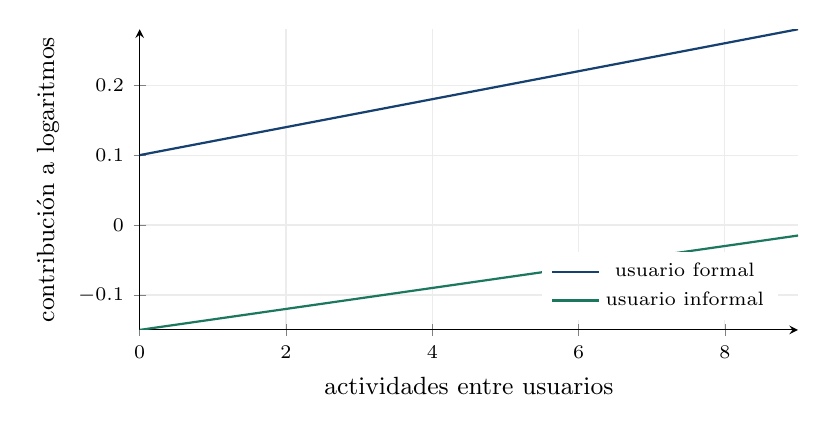
\begin{tikzpicture}\begin{axis}[base,width=.82\textwidth,height=5.4cm,xlabel={actividades entre usuarios},ylabel={contribución a logaritmos},legend pos=south east]
\addplot[azul,thick,domain=0:9]{.1+.02*x};\addlegendentry{usuario formal}
\addplot[verde,thick,domain=0:9]{.1+.02*x-.25-.03-.005*(x-6)};\addlegendentry{usuario informal}
\end{axis}\end{tikzpicture}\caption{Contribuciones ilustrativas del bloque digital en la ecuación literal.}\end{figure}

Las líneas no incluyen el resto del ingreso ajustado; al comparar perfiles iguales esos componentes se cancelan. La figura no atribuye esos números a estimaciones de la tesis.

La asociación del conteo se identifica con variación de intensidad entre usuarios. Si todos los usuarios tuvieran igual conteo, las columnas $A_i$ y $U_i$ serían proporcionales y sus dos pendientes no podrían separarse.

\clearpage
\phantomsection\addcontentsline{toc}{subsection}{Normal bivariada, truncamiento y razón inversa de Mills}
{\large\bfseries\color{azul}Normal bivariada, truncamiento y razón inversa de Mills}\par\vspace{2mm}
\section{Normal estándar: calcular la constante de normalización}

La densidad normal estándar es
\[
\phi(t)=\frac1{\sqrt{2\pi}}e^{-t^2/2}.
\]
Para deducir la constante, consideremos la integral
positiva de \(e^{-t^2/2}\) sobre la recta.
Su cuadrado es una integral doble:
\[
\left[\int_{\mathbb R}e^{-t^2/2}\dd t\right]^2
=\int_{\mathbb R^2}e^{-(u^2+v^2)/2}\dd u\dd v.
\]
El cambio a coordenadas polares,
\(u=r\cos\theta,v=r\sin\theta\),
tiene Jacobiano \(r\). Por tanto,
\[
\int_0^{2\pi}\int_0^\infty e^{-r^2/2}r\dd r\dd\theta
=2\pi[-e^{-r^2/2}]_0^\infty=2\pi.
\]
La integral original es positiva,
así que vale \(\sqrt{2\pi}\).
Dividir por esa cantidad hace área total uno.

La densidad es simétrica:
\(\phi(-t)=\phi(t)\).
Su media es cero porque \(t\phi(t)\)
es impar e integrable.
La derivada de la densidad es
\[
\phi'(t)=-t\phi(t).
\]
Esta identidad permite integrar momentos
sin memorizar fórmulas de una tabla.

Para el segundo momento,
\[
\begin{aligned}
\int_{\mathbb R}t^2\phi(t)\dd t
&=-\int_{\mathbb R}t\phi'(t)\dd t\\
&=-[t\phi(t)]_{-\infty}^{\infty}
+\int_{\mathbb R}\phi(t)\dd t=1.
\end{aligned}
\]
El término de frontera desaparece
por el descenso exponencial.
La varianza estándar es uno.

Si \(\varepsilon_i=\sigma\nu_i\),
con \(\nu_i\) estándar y \(\sigma>0\),
su densidad incorpora el Jacobiano:
\[
f_{\varepsilon_i}(e)
=\frac1\sigma\phi(e/\sigma).
\]
Su esperanza es cero y su varianza \(\sigma^2\).
La división por \(\sigma\) fuera de
la densidad no es opcional:
garantiza normalización después de
cambiar la unidad del error.

\begin{figure}[H]\centering
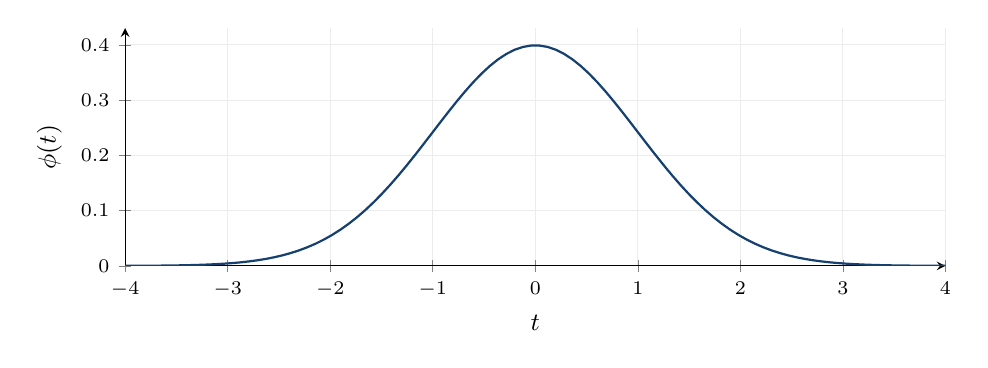
\begin{tikzpicture}\begin{axis}[base,width=12cm,height=4.6cm,xmin=-4,xmax=4,ymin=0,ymax=.43,xlabel={$t$},ylabel={$\phi(t)$}]
\addplot[azul,thick,domain=-4:4]{exp(-x^2/2)/sqrt(2*pi)};
\end{axis}\end{tikzpicture}
\caption{Densidad normal estándar obtenida por normalización.}
\end{figure}


El cambio escalar anterior construye una distribución marginal normal. No impone que el error salarial de Heckman sea exactamente $\sigma\nu_i$. La relación de los dos errores distintos se construye con correlación y una parte independiente en las siguientes unidades.

\clearpage
\section{Distribución acumulada normal: simetría y derivadas de sus argumentos}

La acumulada se define por
\[
\Phi(t)=\int_{-\infty}^t\phi(u)\dd u.
\]
El teorema fundamental del cálculo implica
\(\Phi'(t)=\phi(t)\).
Por simetría de la densidad,
\[
1-\Phi(t)=\Phi(-t).
\]
Para probarlo, cambiar \(u\) por \(-v\)
en la integral de \(t\) a infinito
transforma sus límites en menos infinito y \(-t\).

Para un producto de regresores,
la regla de la cadena da
\[
\frac{\partial}{\partial\pi_l}
\Phi\left(\sum_{h=1}^qZ_{ih}\pi_h\right)
=\phi\left(\left(\sum_{l=1}^{p_Z}Z_{il}\pi_l+\lambda_{y(i)}^{(S)}+\mu_{m(i)}^{(S)}\right)\right)Z_{il}.
\]
La segunda derivada es
\[
-\left(\left(\sum_{l=1}^{p_Z}Z_{il}\pi_l+\lambda_{y(i)}^{(S)}+\mu_{m(i)}^{(S)}\right)\right)
\phi\left(\left(\sum_{l=1}^{p_Z}Z_{il}\pi_l+\lambda_{y(i)}^{(S)}+\mu_{m(i)}^{(S)}\right)\right)
Z_{il}Z_{ir}.
\]
Los datos permanecen fijos.
Una derivada por coeficiente añade
la coordenada correspondiente del dato.

Para el argumento estandarizado
\((w_i-\sum_jW_{ij}\beta_j)/\sigma\),
las derivadas son
\[
-\frac{W_{il}}{\sigma}
\quad\text{respecto de }\beta_l,\qquad
-\frac{w_i-\sum_jW_{ij}\beta_j}{\sigma^2}
\quad\text{respecto de }\sigma.
\]
Estas dos reglas se usarán muchas veces
en Tobit y en la verosimilitud de Heckman.

\begin{ejemplo}[Probabilidad de selección]
Si la suma \(\left(\sum_{l=1}^{p_Z}Z_{il}\pi_l+\lambda_{y(i)}^{(S)}+\mu_{m(i)}^{(S)}\right)\)
vale uno, la selección probit tiene
probabilidad \(\Phi(1)\approx.84134475\).
Su derivada respecto del intercepto
es \(\phi(1)\approx.24197072\).
\end{ejemplo}
La acumulada no se reemplaza por
la densidad: una representa una
probabilidad y la otra su cambio
por unidad del argumento.

En los extremos, la probabilidad
puede acercarse a cero o uno,
mientras la densidad se vuelve pequeña.
Los cocientes de ambas pueden
permanecer grandes y exigir
evaluación numérica estable.


\clearpage
\section{Normal bivariada: construir la matriz de covarianza de dos errores}

Heckman utilizará un error de resultado
\(\varepsilon_i\) y otro de selección \(\nu_i\).
Condicionados en los regresores, supongamos
\[
\begin{pmatrix}\varepsilon_i\\\nu_i\end{pmatrix}
\sim\mathcal N_2\left[
\begin{pmatrix}0\\0\end{pmatrix},
\begin{pmatrix}\sigma^2&\rho\sigma\\\rho\sigma&1\end{pmatrix}
\right],
\quad \sigma>0,\ |\rho|<1.
\]
La varianza del segundo error se fija en uno
para identificar la escala de la ecuación binaria.
La covarianza es \(\rho\sigma\),
no \(\rho\sigma^2\).

El determinante de la matriz es
\(\sigma^2(1-\rho^2)>0\).
Su inversa por cofactores es
\[
\frac1{1-\rho^2}
\begin{pmatrix}
1/\sigma^2&-\rho/\sigma\\
-\rho/\sigma&1
\end{pmatrix}.
\]
La densidad conjunta es
\[
\frac{\exp\left\{
-\frac1{2(1-\rho^2)}
\left[\frac{e^2}{\sigma^2}
-\frac{2\rho ev}{\sigma}+v^2\right]\right\}}
{2\pi\sigma\sqrt{1-\rho^2}}.
\]
El término cruzado determina cómo
se inclinan sus curvas de densidad.

Una construcción equivalente usa
dos normales estándar independientes:
\[
\nu_i\sim\mathcal N(0,1),\quad u_i\sim\mathcal N(0,1),
\qquad
\varepsilon_i=\rho\sigma\nu_i
+\sigma\sqrt{1-\rho^2}\,u_i.
\]
Linealidad de esperanza da media cero.
La varianza es
\(\rho^2\sigma^2+\sigma^2(1-\rho^2)=\sigma^2\).
La covarianza con \(\nu_i\) es \(\rho\sigma\).

Esta construcción permite ver la parte
del error de resultado que comparte
el error de selección y la parte independiente.
Condicionar en un evento de \(\nu_i\)
altera la primera y deja intacta
la distribución de la segunda.

En \(|\rho|=1\), el determinante se anula
y la distribución pierde una dimensión.
Las fórmulas de densidad interior
no se aplican allí por simple sustitución.


\clearpage
\section{Completar cuadrados: derivar ambas normales condicionales}

En la densidad bivariada, completar
el cuadrado en el error de resultado da
\[
\frac{e^2}{\sigma^2}
-\frac{2\rho ev}{\sigma}+v^2
=\left(\frac e\sigma-\rho v\right)^2
+(1-\rho^2)v^2.
\]
Dividir por \(1-\rho^2\) separa
una densidad estándar en \(v\)
y una normal en \(e\) con media
\(\rho\sigma v\) y varianza
\(\sigma^2(1-\rho^2)\).
Por ello,
\[
\varepsilon_i\mid\nu_i=v
\sim\mathcal N(\rho\sigma v,\sigma^2(1-\rho^2)).
\]

Completar el cuadrado en el otro orden produce
\[
\frac{e^2}{\sigma^2}
-\frac{2\rho ev}{\sigma}+v^2
=(v-\rho e/\sigma)^2
+(1-\rho^2)e^2/\sigma^2.
\]
Así,
\[
\nu_i\mid\varepsilon_i=e
\sim\mathcal N(\rho e/\sigma,1-\rho^2).
\]
Se usarán las dos direcciones:
la primera para medias seleccionadas,
la segunda para la densidad conjunta
de resultado observado y selección.

\begin{ejemplo}[Correlación .5 y escala dos]
Condicionado en \(\nu_i=1\),
el error de resultado tiene media uno
y varianza tres.
Condicionado en \(\varepsilon_i=2\),
el error de selección tiene media .5
y varianza .75.
\end{ejemplo}
La correlación determina ambas medias,
pero las escalas de los errores
hacen distintos sus coeficientes.
No se intercambia \(\rho\sigma\)
con \(\rho/\sigma\).

Si \(\rho=0\), la densidad conjunta
factoriza en las dos marginales normales,
y los errores son independientes.
Para distribuciones no normales,
covarianza cero por sí sola
no garantiza esa independencia.

La distribución condicional aquí se
dedujo de una hipótesis bivariada específica.
No es una identidad válida para
cualquier pareja de errores
con la misma matriz de covarianza.


\clearpage
\section{Truncar una normal: obtener la densidad condicional}

Sea \(\nu_i\sim\mathcal N(0,1)\).
Condicionar en \(\nu_i>a\) restringe
los valores posibles, pero debe
mantener área total uno:
\[
f(v\mid\nu_i>a)
=\frac{\phi(v)}{1-\Phi(a)}\mathbf1\{v>a\}.
\]
El denominador es la probabilidad
del evento condicionado.
Integrar la densidad restringida
produce exactamente uno.

En selección probit,
\[
S_i=1\left\{\left(\sum_{l=1}^{p_Z}Z_{il}\pi_l+\lambda_{y(i)}^{(S)}+\mu_{m(i)}^{(S)}\right)+\nu_i>0\right\}.
\]
Manteniendo fijos los regresores,
el evento es
\(\nu_i>-\left(\sum_{l=1}^{p_Z}Z_{il}\pi_l+\lambda_{y(i)}^{(S)}+\mu_{m(i)}^{(S)}\right)\).
Su probabilidad es
\[
1-\Phi\left(-\left(\sum_{l=1}^{p_Z}Z_{il}\pi_l+\lambda_{y(i)}^{(S)}+\mu_{m(i)}^{(S)}\right)\right)
=\Phi\left(\left(\sum_{l=1}^{p_Z}Z_{il}\pi_l+\lambda_{y(i)}^{(S)}+\mu_{m(i)}^{(S)}\right)\right).
\]
Por tanto la densidad seleccionada es
\[
\frac{\phi(v)}
{\Phi(\sum_{l=1}^{p_Z}Z_{il}\pi_l+\lambda_{y(i)}^{(S)}+\mu_{m(i)}^{(S)})}
\mathbf1\left\{v>-\left(\sum_{l=1}^{p_Z}Z_{il}\pi_l+\lambda_{y(i)}^{(S)}+\mu_{m(i)}^{(S)}\right)\right\}.
\]

El soporte cambia con los regresores.
Una baja probabilidad de selección
conserva solamente valores altos
del error \(\nu_i\).
Aunque su distribución original
tenga media cero, su media
entre seleccionados puede ser grande.

\begin{ejemplo}[Selección con intercepto cero]
El evento es \(\nu_i>0\),
y su densidad es \(2\phi(v)\)
para valores positivos.
Su media no es cero:
el lado negativo se ha eliminado.
\end{ejemplo}
Censurar en cero conserva también
una masa para los valores eliminados.
Truncar y condicionar renormaliza
la densidad de los restantes.
Este cociente será central para
derivar Mills por integración.

No se puede convertir una distribución
seleccionada en una normal ordinaria
cambiando únicamente su media:
su forma y su varianza
también cambian con el truncamiento.


\clearpage
\section{Primer momento truncado: la integral que produce Mills}

La media de una normal estándar
condicionada en \(\nu_i>a\) es
\[
\frac{\int_a^\infty v\phi(v)\dd v}
{1-\Phi(a)}.
\]
Usar \(\phi'(v)=-v\phi(v)\)
resuelve el numerador:
\[
\int_a^\infty v\phi(v)\dd v
=-[\phi(v)]_a^\infty=\phi(a).
\]
La densidad tiende a cero en infinito.
La media truncada queda
\[
\E[\nu_i\mid\nu_i>a]
=\frac{\phi(a)}{1-\Phi(a)}.
\]

Para el evento de selección,
el umbral es \(a=-\left(\sum_{l=1}^{p_Z}Z_{il}\pi_l+\lambda_{y(i)}^{(S)}+\mu_{m(i)}^{(S)}\right)\).
La simetría de densidad y acumulada produce
\[
\boxed{
\E[\nu_i\mid Z_i,S_i=1]
=\frac{\phi(\sum_{l=1}^{p_Z}Z_{il}\pi_l+\lambda_{y(i)}^{(S)}+\mu_{m(i)}^{(S)})}
{\Phi(\sum_{l=1}^{p_Z}Z_{il}\pi_l+\lambda_{y(i)}^{(S)}+\mu_{m(i)}^{(S)})}}.
\]
Esta es la razón inversa de Mills
que entra en Heckman.
Su signo es positivo para cualquier
argumento finito.

No es la probabilidad de selección.
En un argumento cero,
la probabilidad es \(1/2\),
pero el cociente es
\[
\frac{1/\sqrt{2\pi}}{1/2}
=\sqrt{2/\pi}\approx.79788456.
\]
Un cociente mayor que uno
no representa una probabilidad inválida:
representa una media condicional de un error.

\begin{ejemplo}[Evento raro]
Si el producto de selección vale \(-2\),
solo se seleccionan errores mayores que dos.
Su media tiene que superar dos.
La razón es aproximadamente \(2.37321553\),
coherente con ese soporte.
\end{ejemplo}
La nueva columna de segunda etapa
resume una media de error derivada
del mecanismo de selección y
de la hipótesis normal.
Su coeficiente en la ecuación
de resultado dependerá de la
covarianza entre ambos errores.

El nombre de la razón no reemplaza
la demostración: apareció al dividir
una integral de primer momento
por la probabilidad del evento.


\clearpage
\section{Segundo momento truncado: integración por partes completa}

El segundo momento condicionado es
\[
\E[\nu_i^2\mid\nu_i>a]
=\frac{\int_a^\infty v^2\phi(v)\dd v}
{1-\Phi(a)}.
\]
Usando la derivada de la densidad,
\[
\begin{aligned}
\int_a^\infty v^2\phi(v)\dd v
&=-\int_a^\infty v\phi'(v)\dd v\\
&=-[v\phi(v)]_a^\infty
+\int_a^\infty\phi(v)\dd v\\
&=a\phi(a)+1-\Phi(a).
\end{aligned}
\]
El término \(v\phi(v)\) se anula
en infinito.
Al dividir queda
\[
\E[\nu_i^2\mid\nu_i>a]
=1+a\frac{\phi(a)}{1-\Phi(a)}.
\]

En selección, sustituir el umbral
\(a=-\left(\sum_{l=1}^{p_Z}Z_{il}\pi_l+\lambda_{y(i)}^{(S)}+\mu_{m(i)}^{(S)}\right)\) produce
\[
\E[\nu_i^2\mid Z_i,S_i=1]
=1-\left(\left(\sum_{l=1}^{p_Z}Z_{il}\pi_l+\lambda_{y(i)}^{(S)}+\mu_{m(i)}^{(S)}\right)\right)
\frac{\phi(\sum_{l=1}^{p_Z}Z_{il}\pi_l+\lambda_{y(i)}^{(S)}+\mu_{m(i)}^{(S)})}
{\Phi(\sum_{l=1}^{p_Z}Z_{il}\pi_l+\lambda_{y(i)}^{(S)}+\mu_{m(i)}^{(S)})}.
\]
La varianza resta el cuadrado
de la media ya deducida:
\[
\boxed{
1-\frac{\phi(\sum_{l=1}^{p_Z}Z_{il}\pi_l+\lambda_{y(i)}^{(S)}+\mu_{m(i)}^{(S)})}
{\Phi(\sum_{l=1}^{p_Z}Z_{il}\pi_l+\lambda_{y(i)}^{(S)}+\mu_{m(i)}^{(S)})}
\left[
\left(\sum_{l=1}^{p_Z}Z_{il}\pi_l+\lambda_{y(i)}^{(S)}+\mu_{m(i)}^{(S)}\right)
+\frac{\phi(\sum_{l=1}^{p_Z}Z_{il}\pi_l+\lambda_{y(i)}^{(S)}+\mu_{m(i)}^{(S)})}
{\Phi(\sum_{l=1}^{p_Z}Z_{il}\pi_l+\lambda_{y(i)}^{(S)}+\mu_{m(i)}^{(S)})}
\right]}.
\]
El segundo momento y la varianza
no son la misma cantidad.

\begin{ejemplo}[Seminormal]
En producto de selección cero,
el segundo momento es uno
y la varianza es \(1-2/\pi\approx.36338023\).
La media positiva explica la diferencia.
\end{ejemplo}
Seleccionar errores de una sola cola
reduce su variación alrededor de
la nueva media bajo este modelo.
No necesariamente reduce el segundo
momento respecto de cero.

La misma expresión dará
heterocedasticidad en la ecuación
de resultado seleccionado.
Sus valores cambiarán entre filas
porque cambia el producto de selección.


\clearpage
\section{Momentos truncados de orden superior: deducir una recurrencia}

Para un entero \(m\ge2\),
usar \(v\phi(v)=-\phi'(v)\)
da la identidad
\[
\begin{aligned}
\int_a^\infty v^m\phi(v)\dd v
&=-\int_a^\infty v^{m-1}\phi'(v)\dd v\\
&=a^{m-1}\phi(a)
+(m-1)\int_a^\infty v^{m-2}\phi(v)\dd v.
\end{aligned}
\]
La integral de orden \(m\) se reduce
a otra de orden \(m-2\).
La frontera en infinito desaparece
porque cualquier potencia fija
por la densidad normal tiende a cero.

Las dos bases son
\[
\int_a^\infty\phi(v)\dd v=1-\Phi(a),
\qquad
\int_a^\infty v\phi(v)\dd v=\phi(a).
\]
Por ejemplo,
\[
\int_a^\infty v^3\phi(v)\dd v
=(a^2+2)\phi(a),
\]
\[
\int_a^\infty v^4\phi(v)\dd v
=(a^3+3a)\phi(a)+3[1-\Phi(a)].
\]
Dividir por la probabilidad de truncamiento
convierte estos numeradores en
momentos condicionados.

Los momentos de tercero y cuarto orden
permiten estudiar asimetría y colas
de las distribuciones seleccionadas.
También aparecen al verificar
información esperada de una escala normal.

\begin{ejemplo}[Umbral cero]
El tercer momento seminormal es
\(2\sqrt{2/\pi}\approx1.59576912\),
y el cuarto es tres.
La asimetría es compatible con
un segundo momento igual al normal original.
\end{ejemplo}
Un modelo seleccionado no queda
completamente descrito por su media
y varianza. La distribución conserva
una forma truncada y puede ser
marcadamente asimétrica.

La recurrencia evita memorizar
cada integral por separado.
Se obtuvieron todos sus términos
mediante una misma integración por partes.


\clearpage
\section{Derivar Mills: cociente, densidad y acumulada}

Consideremos la función escalar
\(\phi(t)/\Phi(t)\).
El cociente tiene denominador positivo
para todo \(t\) finito.
La regla de derivación produce
\[
\begin{aligned}
\frac{\dd}{\dd t}\frac{\phi(t)}{\Phi(t)}
&=\frac{\phi'(t)\Phi(t)-\phi(t)\Phi'(t)}{\Phi(t)^2}\\
&=\frac{-t\phi(t)\Phi(t)-\phi(t)^2}{\Phi(t)^2}\\
&=-\frac{\phi(t)}{\Phi(t)}
\left[t+\frac{\phi(t)}{\Phi(t)}\right].
\end{aligned}
\]
Se utilizaron ambas derivadas,
no solamente la de la densidad.

Al aplicar esta función a datos,
\[
\begin{aligned}
&\frac{\partial}{\partial\pi_l}
\frac{\phi(\sum_{l=1}^{p_Z}Z_{il}\pi_l+\lambda_{y(i)}^{(S)}+\mu_{m(i)}^{(S)})}
{\Phi(\sum_{l=1}^{p_Z}Z_{il}\pi_l+\lambda_{y(i)}^{(S)}+\mu_{m(i)}^{(S)})}\\
&=-\frac{\phi(\sum_{l=1}^{p_Z}Z_{il}\pi_l+\lambda_{y(i)}^{(S)}+\mu_{m(i)}^{(S)})}
{\Phi(\sum_{l=1}^{p_Z}Z_{il}\pi_l+\lambda_{y(i)}^{(S)}+\mu_{m(i)}^{(S)})}
\left[
\left(\sum_{l=1}^{p_Z}Z_{il}\pi_l+\lambda_{y(i)}^{(S)}+\mu_{m(i)}^{(S)}\right)+
\frac{\phi(\sum_{l=1}^{p_Z}Z_{il}\pi_l+\lambda_{y(i)}^{(S)}+\mu_{m(i)}^{(S)})}
{\Phi(\sum_{l=1}^{p_Z}Z_{il}\pi_l+\lambda_{y(i)}^{(S)}+\mu_{m(i)}^{(S)})}
\right]Z_{il}.
\end{aligned}
\]
Cada fila conserva sus propios datos.
La coordenada \(Z_{il}\) entra
por la regla de la cadena.

La derivada del logaritmo de la acumulada
es la razón misma:
\[
\frac{\dd}{\dd t}\log\Phi(t)=\frac{\phi(t)}{\Phi(t)}.
\]
Por ello la derivada de Mills
es la segunda derivada de \(\log\Phi\).
Esta conexión determina
la curvatura de probit y Tobit.

\begin{ejemplo}[Centro]
En \(t=0\), la derivada es \(-2/\pi\).
Un pequeño aumento del argumento
disminuye la media del error seleccionado:
la selección se vuelve menos exigente.
\end{ejemplo}
La derivada no es constante.
Usar siempre el valor del centro
en un probit o en una corrección de selección
reemplazaría la función por
una aproximación local que
puede ser mala en las colas.


\clearpage
\section{Signo de Mills y cota de su derivada mediante una varianza}

La razón \(\phi(t)/\Phi(t)\) es positiva.
Además,
\[
t+\frac{\phi(t)}{\Phi(t)}>0.
\]
Para \(t\ge0\), esto es inmediato.
Para \(t<0\), la razón es
la media de una normal condicionada
a superar \(-t>0\).
Como todos sus valores superan
ese umbral, su media también lo supera.

La derivada deducida es entonces negativa:
\[
\frac{\dd}{\dd t}\frac{\phi(t)}{\Phi(t)}<0.
\]
La varianza truncada satisface
\[
\Var(\nu_i\mid\nu_i>-t)
=1+\frac{\dd}{\dd t}\frac{\phi(t)}{\Phi(t)}.
\]
Es estrictamente positiva para
un argumento finito, pues la
distribución no es degenerada.
Por tanto,
\[
-1<
\frac{\dd}{\dd t}\frac{\phi(t)}{\Phi(t)}
<0.
\]
Esta cota no se obtuvo observando
un gráfico, sino conectando
la derivada con una varianza.

La positividad de la varianza
también implica que
\[
0<
\frac{\phi(t)}{\Phi(t)}
\left[t+\frac{\phi(t)}{\Phi(t)}\right]
<1.
\]
El factor será utilizado
para reducir la varianza del
error de resultado seleccionado.

\begin{ejemplo}[Interpretación de la pendiente]
Al incrementar el producto de selección,
la media del error truncado baja.
Su pendiente nunca es menor que \(-1\)
bajo la distribución normal.
\end{ejemplo}
Las cotas ayudan a comprobar
signos de Hessianas y a detectar
errores de implementación.
Un valor de varianza negativo
en una cola puede indicar
cancelación o redondeo numérico,
y no una propiedad real del modelo.

La cota pertenece a esta
razón normal específica.
No se transporta a cualquier
función de corrección de selección
sin deducir sus propios momentos.


\clearpage
\section{Segunda derivada de Mills: abrir producto y cadena}

Derivemos otra vez la identidad
\[
-\frac{\phi(t)}{\Phi(t)}
\left[t+\frac{\phi(t)}{\Phi(t)}\right].
\]
La regla del producto da
\[
\begin{aligned}
&-\left(\frac{\phi(t)}{\Phi(t)}\right)'
\left[t+\frac{\phi(t)}{\Phi(t)}\right]\\
&-\frac{\phi(t)}{\Phi(t)}
\left[1+\left(\frac{\phi(t)}{\Phi(t)}\right)'\right].
\end{aligned}
\]
Sustituir la primera derivada
y reunir términos produce
\[
\boxed{
\frac{\dd^2}{\dd t^2}\frac{\phi(t)}{\Phi(t)}
=\frac{\phi(t)}{\Phi(t)}
\left[
\left(t+\frac{\phi(t)}{\Phi(t)}\right)
\left(t+2\frac{\phi(t)}{\Phi(t)}\right)-1
\right]}.
\]
Cada producto es escalar.
Al usar un argumento lineal en \(\pi\),
la segunda derivada cruzada multiplica
esta expresión por \(Z_{il}Z_{ir}\).

Esta fórmula permite calcular
cómo cambia el Jacobiano de
una segunda etapa al mover
parámetros de primera etapa.
También controla restos de Taylor
en una vecindad finita.

\begin{ejemplo}[Evaluación en cero]
Con \(\phi(0)/\Phi(0)=\sqrt{2/\pi}\),
la segunda derivada es
\[
\sqrt{2/\pi}\left(\frac4\pi-1\right)
\approx.21801361.
\]
La primera derivada en el mismo punto
es aproximadamente \(-.63661977\).
\end{ejemplo}
Las funciones y sus derivadas
deben evaluarse en el argumento
completo de cada fila.
Dos registros con probabilidades
parecidas pueden tener sensibilidades
distintas si sus coordenadas
\(Z_{il}\) son distintas.

Para una función vectorial
de todas las razones,
el Jacobiano tiene una fila
por observación y una columna
por coeficiente de selección.
Ese tamaño debe conservarse
al propagar la covarianza de \(\widehat\pi\).


\clearpage
\section{Mills en la cola: deducir cotas por integración por partes}

Para \(a>0\), la cola normal superior es
\(\int_a^\infty\phi(v)\dd v\).
Como \(v/a\ge1\),
\[
1-\Phi(a)<\frac1a\int_a^\infty v\phi(v)\dd v
=\frac{\phi(a)}a.
\]
La desigualdad es estricta
porque la densidad tiene masa
en valores mayores que \(a\).

Integrar por partes de otra forma da
\[
1-\Phi(a)=\frac{\phi(a)}a
-\int_a^\infty\frac{\phi(v)}{v^2}\dd v.
\]
El último integral no supera
\([1-\Phi(a)]/a^2\).
Reunir términos implica
\[
1-\Phi(a)>
\frac{a}{a^2+1}\phi(a).
\]
Al invertir las dos cotas positivas,
\[
\boxed{
a<\frac{\phi(a)}{1-\Phi(a)}<a+\frac1a}.
\]
Para el argumento \(t=-a\),
la razón de Mills de selección
queda acotada por esas cantidades.

La relación explica por qué
el cociente es grande cuando
la probabilidad de selección
es muy pequeña: solo sobreviven
errores en una cola alta.
No significa que la densidad
por sí sola sea grande.

\begin{ejemplo}[Argumento menos cinco]
Las cotas son cinco y 5.2.
La razón real es aproximadamente 5.18650397.
Ambos factores originales,
densidad y acumulada inferior,
son pequeños, pero su cociente
no lo es.
\end{ejemplo}
Las cotas permiten validar
un cálculo de cola sin
reproducir toda la integral.
Si una rutina devuelve cero
para esa razón, ha perdido
información por subdesbordamiento.

Para varianzas truncadas extremas,
restar cantidades casi iguales
puede requerir métodos de evaluación
más precisos que la fórmula directa.


\clearpage
\section{Evaluación estable de Mills y probabilidades extremas}

La expresión directa
\(\phi(t)/\Phi(t)\) puede perder precisión
si ambos factores son muy pequeños.
Una forma estable trabaja con logaritmos:
\[
\frac{\phi(t)}{\Phi(t)}
=\exp\left[-\frac{t^2}{2}
-\frac12\log(2\pi)-\log\Phi(t)\right].
\]
El valor \(\log\Phi(t)\) debe
evaluarse con un método de cola,
y no tomando el logaritmo
de un cero redondeado previamente.

Para probabilidades del complemento,
la identidad \(1-\Phi(t)=\Phi(-t)\)
evita restar de uno una
acumulada extremadamente próxima a uno.
La misma regla se aplica
en la log-verosimilitud de
selección no observada.

En una cola con \(t\ll0\),
la razón se aproxima a \(-t\),
con correcciones pequeñas.
La varianza truncada contiene
la diferencia entre uno
y un producto próximo a uno.
Esa cancelación puede perder
dígitos en cálculo ordinario.

\begin{ejemplo}[Una selección extremadamente rara]
Con \(t=-8\),
\(\Phi(t)\approx6.22096\cdot10^{-16}\).
Mills es aproximadamente 8.12136811,
y la varianza truncada aproximadamente .01432488.
Estos números son positivos y
coherentes con las cotas de cola.
\end{ejemplo}
La fórmula matemática sigue válida
en toda la recta real finita.
Una dificultad de aritmética
no modifica el modelo:
requiere una evaluación mejor
de la misma función.

En los laboratorios se calcularán
las razones con la forma logarítmica,
y se verificarán sus momentos
contra integración numérica
cuando la cola lo permita.

Redondear una probabilidad en
una tabla a cero no significa
que su probabilidad matemática
sea cero. La distinción es
especialmente relevante al calcular
derivadas y verosimilitudes.


\clearpage
\section{Seminormal: resolver sus momentos y su asimetría}

La normal condicionada en ser positiva
tiene densidad \(2\phi(v)\)
para \(v>0\).
Sus dos primeros momentos son
\[
\E[\nu_i\mid\nu_i>0]=\sqrt{2/\pi},
\qquad
\E[\nu_i^2\mid\nu_i>0]=1.
\]
Su varianza es
\(1-2/\pi\).
La recurrencia de momentos da
tercer momento \(2\sqrt{2/\pi}\)
y cuarto momento tres.

Para calcular el tercer momento central,
abrir el cubo produce
\[
\begin{aligned}
&\E[(\nu_i-\sqrt{2/\pi})^3\mid\nu_i>0]\\
&=2\sqrt{2/\pi}
-3\sqrt{2/\pi}
+3(2/\pi)\sqrt{2/\pi}
-(2/\pi)^{3/2}\\
&=\sqrt{2/\pi}\left(\frac4\pi-1\right).
\end{aligned}
\]
Dividir por \((1-2/\pi)^{3/2}\)
da su coeficiente de asimetría.

La distribución tiene soporte positivo,
pero una cola derecha infinita.
Una normal ordinaria con la misma
media y varianza tendría soporte
en toda la recta.
Igualar momentos no iguala
las distribuciones.

\begin{ejemplo}[Error de selección con índice cero]
La selección toma exactamente
la mitad superior del error.
Su media .79788456
y varianza .36338023
se obtienen sin estimación alguna
si el parámetro de selección es conocido.
\end{ejemplo}
En Heckman, el error de resultado
es la suma de una parte
proporcional a este error truncado
y otra normal independiente.
Si la correlación no es cero,
su distribución seleccionada
también puede ser asimétrica.

La segunda etapa utiliza correctamente
su media y su varianza
bajo las hipótesis del modelo,
pero no presupone que la
distribución residual seleccionada
sea una normal homocedástica ordinaria.


\clearpage
\section{Truncamiento entre dos límites: normalizar y calcular dos momentos}

Si \(a<\nu_i<b\), la probabilidad del evento es
\(\Phi(b)-\Phi(a)>0\).
La densidad condicionada es
\[
\frac{\phi(v)}{\Phi(b)-\Phi(a)}
\mathbf1\{a<v<b\}.
\]
La integral de primer momento
usa la misma derivada normal:
\[
\int_a^b v\phi(v)\dd v
=\phi(a)-\phi(b).
\]
Por tanto,
\[
\E[\nu_i\mid a<\nu_i<b]
=\frac{\phi(a)-\phi(b)}
{\Phi(b)-\Phi(a)}.
\]
La integración por partes de orden dos produce
\[
\int_a^b v^2\phi(v)\dd v
=a\phi(a)-b\phi(b)+\Phi(b)-\Phi(a).
\]
Al dividir y restar el cuadrado de la media,
\[
\begin{aligned}
\Var(\nu_i\mid a<\nu_i<b)
={}&1+\frac{a\phi(a)-b\phi(b)}
{\Phi(b)-\Phi(a)}\\
&-\left[\frac{\phi(a)-\phi(b)}
{\Phi(b)-\Phi(a)}\right]^2.
\end{aligned}
\]
Los dos términos de frontera importan.
Eliminar uno convertiría el evento
en una truncación de una sola cola.

\begin{ejemplo}[Intervalo simétrico]
Con \(a=-1,b=1\), la media es cero
porque las densidades de frontera
son iguales. La varianza es
\[
1-\frac{2\phi(1)}{\Phi(1)-\Phi(-1)}
\approx.29112509.
\]
\end{ejemplo}
Estas fórmulas se usan en modelos
con límites inferiores y superiores,
y en datos que llegan solo
dentro de una ventana de valores.

Una censura de dos lados
conserva masas en los límites.
La distribución de los registros
interiores condicionados sí tiene
el denominador de esta unidad.
La verosimilitud del conjunto censurado
no lo agrega automáticamente
a cada observación interior.


\clearpage
\section{Probit: derivar gradiente y Hessiana con la razón normal completa}

Con \(S_i\) observado en todas las filas,
la probabilidad de selección es
\(\Phi(\sum_{l=1}^{p_Z}Z_{il}\pi_l+\lambda_{y(i)}^{(S)}+\mu_{m(i)}^{(S)})\).
Su log-verosimilitud es
\[
\sum_i\left[
S_i\log\Phi(\sum_{l=1}^{p_Z}Z_{il}\pi_l+\lambda_{y(i)}^{(S)}+\mu_{m(i)}^{(S)})
+(1-S_i)\log\Phi(-\left(\sum_{l=1}^{p_Z}Z_{il}\pi_l+\lambda_{y(i)}^{(S)}+\mu_{m(i)}^{(S)}\right))\right].
\]
Derivar respecto de \(\pi_r\) da
\[
\sum_i Z_{ir}\left[
S_i\frac{\phi(\sum_{l=1}^{p_Z}Z_{il}\pi_l+\lambda_{y(i)}^{(S)}+\mu_{m(i)}^{(S)})}
{\Phi(\sum_{l=1}^{p_Z}Z_{il}\pi_l+\lambda_{y(i)}^{(S)}+\mu_{m(i)}^{(S)})}
-(1-S_i)\frac{\phi(-\left(\sum_{l=1}^{p_Z}Z_{il}\pi_l+\lambda_{y(i)}^{(S)}+\mu_{m(i)}^{(S)}\right))}
{\Phi(-\left(\sum_{l=1}^{p_Z}Z_{il}\pi_l+\lambda_{y(i)}^{(S)}+\mu_{m(i)}^{(S)}\right))}
\right].
\]
El signo negativo del segundo término
proviene de su argumento negativo.
La densidad es simétrica,
pero sus dos acumuladas no son iguales.

La segunda derivada entre coordenadas \(r,h\)
es la suma de \(Z_{ir}Z_{ih}\)
por la derivada de Mills
en el argumento correspondiente.
Ambos signos de cadena se multiplican,
por lo que el término no seleccionado
también tiene curvatura negativa.

Con la derivada de Mills entre \(-1,0\),
la Hessiana es semidefinida negativa.
Con rango completo y parámetros finitos,
es definida negativa.
La concavidad no garantiza por sí sola
existencia de un máximo finito
si los datos separan selección.

\begin{ejemplo}[Inicio cero]
En \(\pi=0,\lambda^{(S)}=0,\mu^{(S)}=0\), cada probabilidad es \(1/2\).
El gradiente es
\[
\sqrt{2/\pi}\sum_i Z_i(2S_i-1),
\]
y el negativo de la Hessiana es
\[
\frac2\pi\sum_i Z_iZ_i\T.
\]
\end{ejemplo}
La primera etapa de Heckman utilizará
este objetivo sobre seleccionados
y no seleccionados juntos.
Excluir estos últimos antes del probit
impediría estimar el mecanismo
de selección de la población observada.


Las derivadas de calendario tienen la misma forma, con $Z_{ir}$ reemplazado por
$\mathbf1\{y(i)=a\}$ o $\mathbf1\{m(i)=r\}$. Cuando se apila el gradiente se conservan todas esas coordenadas, no solo $\pi$.

\clearpage
\phantomsection\addcontentsline{toc}{subsection}{Heckman pooled, selección y las dos etapas completas}
{\large\bfseries\color{azul}Heckman pooled, selección y las dos etapas completas}\par\vspace{2mm}
\section{Normalizar la escala de participación sin normalizar salarios}

Multiplicar $S_i^*$ por $c>0$ no cambia $\mathbf1\{S_i^*>0\}$. Una ecuación binaria con error de varianza desconocida identifica las pendientes divididas por la desviación del error, no las dos magnitudes por separado.
\[
\Prob(S_i=1\mid Z_i)
=\Phi\left(
\frac{Z_i^{\mathsf T}\pi+\lambda_{y(i)}^{(S)}+\mu_{m(i)}^{(S)}}
{\sqrt{\Var(\nu_i)}}\right).
\]
Se fija $\Var(\nu_i)=1$. La escala salarial $\sigma$ se conserva como parámetro porque el logaritmo del ingreso se observa con unidades determinadas.

La matriz normal conjunta es
\[
\begin{pmatrix}\sigma^2&\rho\sigma\\\rho\sigma&1\end{pmatrix}.
\]
La descomposición
$\varepsilon_i^{(0)}=\rho\sigma\nu_i+
\sigma\sqrt{1-\rho^2}\,u_i$
con $u_i$ estándar independiente de $\nu_i$ reproduce todas sus entradas:
$\Var(\varepsilon_i^{(0)})=\rho^2\sigma^2+\sigma^2(1-\rho^2)=\sigma^2$.

En la simulación posterior $u_i$ es un error de generación, no una variable explicativa añadida a la tesis. Los regresores de las ecuaciones permanecen iguales.

\clearpage
\section{Derivar la probabilidad de selección desde el indicador}
Partiendo del umbral, se obtiene
\[
\begin{aligned}
\Prob(S_i=1\mid Z_i,y(i),m(i))
&=\Prob\left(\nu_i>-(\sum_{l=1}^{p_Z}Z_{il}\pi_l+\lambda_{y(i)}^{(S)}+\mu_{m(i)}^{(S)})\right)\\
&=1-\Phi\left(-(\sum_{l=1}^{p_Z}Z_{il}\pi_l+\lambda_{y(i)}^{(S)}+\mu_{m(i)}^{(S)})\right)\\
&=\Phi\left(\sum_{l=1}^{p_Z}Z_{il}\pi_l+\lambda_{y(i)}^{(S)}+\mu_{m(i)}^{(S)}\right).
\end{aligned}
\]

La segunda igualdad usa la normal estándar del error de selección y la tercera, su simetría. La probabilidad de no selección es la acumulada del argumento negativo.

El probit se estima sobre todas las filas con $S_i$ y regresores disponibles. Si se eliminaran todos los ceros, la log-verosimilitud sería una suma de logaritmos de probabilidades de uno y podría aumentar llevando el intercepto hacia infinito.

Las dummies temporales de selección controlan diferencias de observabilidad por año y estacionalidad. No se presume que esos parámetros coincidan con diferencias salariales.

La marginal de $S_i$ no incluye $\rho$ ni $\sigma$. Esos parámetros intervienen en la relación entre error salarial y selección, no en la distribución marginal de un error de selección normalizado.

\clearpage
\section{Media seleccionada del error salarial mediante dos esperanzas}
La esperanza iterada condicional produce
\[
\begin{aligned}
\E[\varepsilon_i^{(0)}\mid W_i,Z_i,S_i=1]
&=\E[\E[\varepsilon_i^{(0)}\mid\nu_i,W_i,Z_i]\mid W_i,Z_i,S_i=1]\\
&=\rho\sigma\,\E[\nu_i\mid\nu_i>-(\sum_{l=1}^{p_Z}Z_{il}\pi_l+\lambda_{y(i)}^{(S)}+\mu_{m(i)}^{(S)})]\\
&=\rho\sigma\,\frac{\phi\!\left(\sum_{l=1}^{p_Z}Z_{il}\pi_l+\lambda_{y(i)}^{(S)}+\mu_{m(i)}^{(S)}\right)}{\Phi\!\left(\sum_{l=1}^{p_Z}Z_{il}\pi_l+\lambda_{y(i)}^{(S)}+\mu_{m(i)}^{(S)}\right)}.
\end{aligned}
\]

La primera esperanza interior es $\rho\sigma\nu_i$, demostrada completando cuadrados de la normal bivariada. La media normal truncada se obtuvo por integrar $v\phi(v)$ en el intervalo de selección.

Así surge Mills como una esperanza de un error seleccionado. No es una variable elegida para mejorar arbitrariamente el ajuste. Su argumento contiene los mismos parámetros y datos del probit.

El coeficiente salarial de la razón es
\[
\kappa=\rho\sigma.
\]
Si $\rho>0$, los errores salariales observados tienen media positiva. Si $\rho<0$, es negativa. Si $\rho=0$, la media seleccionada es cero, aunque el ingreso observable siga siendo un subconjunto de la población.

\clearpage
\section{El error corregido y su varianza heterocedástica}

Definir el error corregido por una igualdad:
\[
\varepsilon_i=
\varepsilon_i^{(0)}
-\rho\sigma\frac{\phi(Z_i^{\mathsf T}\pi+\lambda_{y(i)}^{(S)}+\mu_{m(i)}^{(S)})}
{\Phi(Z_i^{\mathsf T}\pi+\lambda_{y(i)}^{(S)}+\mu_{m(i)}^{(S)})},
\quad S_i=1.
\]
Su media seleccionada es cero. Restar una media no cambia la varianza seleccionada.

Con la descomposición del error y la varianza normal truncada:
\[
\begin{aligned}
\Var(\varepsilon_i\mid W_i,Z_i,S_i=1)
=\sigma^2\Bigg[1-\rho^2&
\frac{\phi(Z_i^{\mathsf T}\pi+\lambda_{y(i)}^{(S)}+\mu_{m(i)}^{(S)})}
{\Phi(Z_i^{\mathsf T}\pi+\lambda_{y(i)}^{(S)}+\mu_{m(i)}^{(S)})}\\
\cdot\Bigg(&Z_i^{\mathsf T}\pi+\lambda_{y(i)}^{(S)}+\mu_{m(i)}^{(S)}
+\frac{\phi(Z_i^{\mathsf T}\pi+\lambda_{y(i)}^{(S)}+\mu_{m(i)}^{(S)})}
{\Phi(Z_i^{\mathsf T}\pi+\lambda_{y(i)}^{(S)}+\mu_{m(i)}^{(S)})}\Bigg)\Bigg].
\end{aligned}
\]
La cantidad entre corchetes está entre $1-\rho^2$ y uno. Con $\abs\rho<1$ es positiva. Depende de los regresores de selección, de modo que la segunda etapa tiene heterocedasticidad aun si la normal salarial original tiene varianza constante.

Una fórmula homocedástica de MCO sobre la segunda etapa ignora esa estructura y la estimación del regresor de Mills.

\clearpage
\section{Sesgo de la ecuación principal cuando se omite la selección}

En las filas seleccionadas, la media del resultado es
\[
\sum_jW_{ij}\beta_j+
\kappa\frac{\phi(Z_i^{\mathsf T}\pi+\lambda_{y(i)}^{(S)}+\mu_{m(i)}^{(S)})}
{\Phi(Z_i^{\mathsf T}\pi+\lambda_{y(i)}^{(S)}+\mu_{m(i)}^{(S)})}.
\]
Si se ajusta la ecuación principal sin la corrección, su esperanza condicional al diseño y al patrón de selección es
\[
\begin{aligned}
\E[\widehat\beta_{\text{sin corrección}}\mid W,Z,S]-\beta
={}&\kappa\left[\sum_{S_i=1}W_iW_i^{\mathsf T}\right]^{-1}\\
&\cdot\sum_{S_i=1}W_i
\frac{\phi(Z_i^{\mathsf T}\pi+\lambda_{y(i)}^{(S)}+\mu_{m(i)}^{(S)})}
{\Phi(Z_i^{\mathsf T}\pi+\lambda_{y(i)}^{(S)}+\mu_{m(i)}^{(S)})}.
\end{aligned}
\]
Cada coordenada del vector puede absorber parte de esa proyección: uso, intensidad, informalidad, sus interacciones, controles y calendario.

La media seleccionada positiva no obliga a que el sesgo de cada pendiente sea positivo. El intercepto, la correlación parcial con cada columna y la inversa del producto cruzado determinan sus signos.

Si $\kappa=0$ desaparece este sesgo específico. Si Mills es constante, su proyección puede recaer en el intercepto y ser colineal con él, impidiendo identificar un coeficiente adicional independiente.

\clearpage
\section{La primera etapa con todas las coordenadas y sus ecuaciones normales}

El vector de parámetros de selección contiene $\pi$ y los dos efectos de año y once de mes. Su diseño tiene fila
\[
\left(Z_i^{\mathsf T},\mathbf1\{y(i)=2024\},\mathbf1\{y(i)=2025\},
(\mathbf1\{m(i)=r\})_{r=2}^{12}\right).
\]
La log-verosimilitud es
\[
\begin{aligned}
\sum_iS_i\ln\Phi(Z_i^{\mathsf T}\pi+\lambda_{y(i)}^{(S)}+\mu_{m(i)}^{(S)})
&+\sum_i(1-S_i)\\
\cdot\ln\Phi(-Z_i^{\mathsf T}\pi-\lambda_{y(i)}^{(S)}-\mu_{m(i)}^{(S)}).
\end{aligned}
\]
Derivar $\pi_l$ multiplica por $Z_{il}$. Derivar $\lambda_{2024}^{(S)}$ multiplica por $\mathbf1\{y(i)=2024\}$. Derivar $\mu_2^{(S)}$ multiplica por $\mathbf1\{m(i)=2\}$.

Todos esos scores se igualan a cero simultáneamente. La cantidad de seleccionados de un mes no basta para estimar su coeficiente si los otros regresores varían dentro de ese mes.

El negativo de la Hessiana reúne productos de todas las columnas de selección, ponderados por la derivada negativa de Mills en el argumento de la fila. Concavidad y existencia de un máximo finito son cuestiones distintas cuando puede haber separación.

\clearpage
\section{Información del probit y covarianza de todos los coeficientes de selección}
El peso esperado de la información en cada fila es
\[
\frac{\phi(\sum_{l=1}^{p_Z}Z_{il}\pi_l+\lambda_{y(i)}^{(S)}+\mu_{m(i)}^{(S)})^2}{\Phi(\sum_{l=1}^{p_Z}Z_{il}\pi_l+\lambda_{y(i)}^{(S)}+\mu_{m(i)}^{(S)})\Phi(-(\sum_{l=1}^{p_Z}Z_{il}\pi_l+\lambda_{y(i)}^{(S)}+\mu_{m(i)}^{(S)}))}.
\]

Multiplica el producto exterior de la fila completa de selección. Por ejemplo, las entradas entre dos $\pi$, entre $\pi$ y año y entre dos meses son
\[
\begin{aligned}
\sum_iZ_{il}Z_{ih}
&\frac{\phi(Z_i^{\mathsf T}\pi+\lambda_{y(i)}^{(S)}+\mu_{m(i)}^{(S)})^2}
{\Phi(Z_i^{\mathsf T}\pi+\lambda_{y(i)}^{(S)}+\mu_{m(i)}^{(S)})
\Phi(-Z_i^{\mathsf T}\pi-\lambda_{y(i)}^{(S)}-\mu_{m(i)}^{(S)})},\\
\sum_{y(i)=2024}Z_{il}
&\frac{\phi(Z_i^{\mathsf T}\pi+\lambda_{y(i)}^{(S)}+\mu_{m(i)}^{(S)})^2}
{\Phi(Z_i^{\mathsf T}\pi+\lambda_{y(i)}^{(S)}+\mu_{m(i)}^{(S)})
\Phi(-Z_i^{\mathsf T}\pi-\lambda_{y(i)}^{(S)}-\mu_{m(i)}^{(S)})}.
\end{aligned}
\]
La entrada entre dos meses distintos es cero porque sus indicadores son excluyentes. Sus covarianzas de estimadores no tienen por qué ser cero: la inversión de la información completa puede generar cruces.

Bajo especificación correcta, la inversa de la suma de información estima la covarianza de primer orden de todos los parámetros de selección. No se toma la inversa de cada diagonal por separado.

No hay una fórmula general que haga exactamente insesgado al estimador probit en muestra finita. Consistencia y normalidad asintótica no se presentan como igualdades exactas de sus esperanzas.

\clearpage
\section{Todas las derivadas de Mills respecto de selección y calendario}
Para un parámetro de selección $\pi_l$, la derivada es
\[
-\frac{\phi\!\left(\sum_{l=1}^{p_Z}Z_{il}\pi_l+\lambda_{y(i)}^{(S)}+\mu_{m(i)}^{(S)}\right)}{\Phi\!\left(\sum_{l=1}^{p_Z}Z_{il}\pi_l+\lambda_{y(i)}^{(S)}+\mu_{m(i)}^{(S)}\right)}\left[\sum_{l=1}^{p_Z}Z_{il}\pi_l+\lambda_{y(i)}^{(S)}+\mu_{m(i)}^{(S)}+\frac{\phi\!\left(\sum_{l=1}^{p_Z}Z_{il}\pi_l+\lambda_{y(i)}^{(S)}+\mu_{m(i)}^{(S)}\right)}{\Phi\!\left(\sum_{l=1}^{p_Z}Z_{il}\pi_l+\lambda_{y(i)}^{(S)}+\mu_{m(i)}^{(S)}\right)}\right]Z_{il}.
\]

Para un efecto de año o mes, se reemplaza la última coordenada por su dummy:
\[
\begin{aligned}
\frac{\partial\widehat\lambda_i}{\partial\lambda_a^{(S)}}
&=-\frac{\phi(Z_i^{\mathsf T}\pi+\lambda_{y(i)}^{(S)}+\mu_{m(i)}^{(S)})}
{\Phi(Z_i^{\mathsf T}\pi+\lambda_{y(i)}^{(S)}+\mu_{m(i)}^{(S)})}\\
&\quad\cdot\left[Z_i^{\mathsf T}\pi+\lambda_{y(i)}^{(S)}+\mu_{m(i)}^{(S)}
+\frac{\phi(Z_i^{\mathsf T}\pi+\lambda_{y(i)}^{(S)}+\mu_{m(i)}^{(S)})}
{\Phi(Z_i^{\mathsf T}\pi+\lambda_{y(i)}^{(S)}+\mu_{m(i)}^{(S)})}\right]\mathbf1\{y(i)=a\}.
\end{aligned}
\]
La expresión se evalúa en los parámetros estimados al calcular un Jacobiano. El sombrero del nombre de la razón no convierte la derivada en cero.

El Jacobiano de todas las razones tiene $n$ filas y $p_Z+13$ columnas. Las covarianzas aproximadas entre razones de personas distintas se obtienen con sus dos filas y la covarianza conjunta del probit. Comparten una estimación de selección y, por ello, pueden estar correlacionadas aun si sus errores originales son independientes.

\clearpage
\section{La segunda etapa ampliada conserva la matriz principal entera}
Cada fila seleccionada de la matriz ampliada es
\[
\left(W_i^{\mathsf T}, \frac{\phi\!\left(\sum_{l=1}^{p_Z}Z_{il}\widehat\pi_l+\widehat\lambda_{y(i)}^{(S)}+\widehat\mu_{m(i)}^{(S)}\right)}{\Phi\!\left(\sum_{l=1}^{p_Z}Z_{il}\widehat\pi_l+\widehat\lambda_{y(i)}^{(S)}+\widehat\mu_{m(i)}^{(S)}\right)}\right).
\]

El vector de coeficientes es $(\beta^{\mathsf T},\kappa)^{\mathsf T}$. El bloque superior izquierdo de su producto cruzado es $\sum_{S_i=1}W_iW_i^{\mathsf T}$; la columna cruzada y la esquina inferior son
\[
\sum_{S_i=1}W_i\widehat\lambda_i,\qquad
\sum_{S_i=1}\widehat\lambda_i^2.
\]
Aquí la razón se despliega con $\phi/\Phi$ en las expresiones siguientes y en los cálculos numéricos. La notación $\widehat\lambda_i$ proviene del apartado (12) de la tesis.
\[
\begin{pmatrix}
\sum_{S_i=1}W_iW_i^{\mathsf T}&\sum_{S_i=1}W_i\widehat\lambda_i\\
\sum_{S_i=1}\widehat\lambda_iW_i^{\mathsf T}&\sum_{S_i=1}\widehat\lambda_i^2
\end{pmatrix}
\begin{pmatrix}\widehat\beta\\\widehat\kappa\end{pmatrix}
=
\begin{pmatrix}\sum_{S_i=1}W_iw_i\\\sum_{S_i=1}\widehat\lambda_iw_i\end{pmatrix}.
\]
La matriz tiene dimensión $p_P+1$, no tres. Las cinco columnas digitales, los bloques $x_{i1}$ y $x_{i2}$ y los efectos temporales permanecen en $W_i$.

El residuo corregido se obtiene restando ambas contribuciones del resultado seleccionado. Su suma y sus productos con todas las columnas ampliadas son cero en el ajuste de mínimos cuadrados.

\clearpage
\section{Esperanza y covarianza si los parámetros de selección fueran conocidos}

Para una razón evaluada en parámetros verdaderos, la ecuación ampliada tiene media correcta. Condicionando al diseño y al patrón, sus coeficientes son insesgados si hay rango completo:
\[
\E\left[\begin{pmatrix}\widehat\beta\\\widehat\kappa\end{pmatrix}\Bigm|W,Z,S\right]
=\begin{pmatrix}\beta\\\kappa\end{pmatrix}.
\]
Para escribir su covarianza exacta, la fila completa ampliada es
\[
\begin{pmatrix}
W_i\\
\phi(Z_i^{\mathsf T}\pi+\lambda_{y(i)}^{(S)}+\mu_{m(i)}^{(S)})
/\Phi(Z_i^{\mathsf T}\pi+\lambda_{y(i)}^{(S)}+\mu_{m(i)}^{(S)})
\end{pmatrix}.
\]
La covarianza se calcula como la inversa de la suma de productos exteriores de estas filas, por la suma de los mismos productos ponderados por
$\Var(\varepsilon_i\mid W,Z,S_i=1)$, por la misma inversa.

Los términos cruzados con Mills contienen una potencia de la razón; la esquina de la matriz central contiene dos. Cada contribución se pondera por su varianza seleccionada, ya deducida.

Esta es una comparación teórica. En el procedimiento real los parámetros se estiman, de modo que ni la insesgadez finita ni esa covarianza conocida se trasladan automáticamente a dos etapas.

\clearpage
\section{Recuperar sigma y rho a partir de los momentos corregidos}

La varianza seleccionada de los residuos corregidos es
$\sigma^2-\kappa^2\lambda_i(\lambda_i+Z_i^{\mathsf T}\pi+
\lambda_{y(i)}^{(S)}+\mu_{m(i)}^{(S)})$. Al promediar:
\[
\begin{aligned}
\widehat\sigma^2={}&
\frac1{n_S}\sum_{S_i=1}\widehat\varepsilon_i^2\\
&+\frac{\widehat\kappa^2}{n_S}\sum_{S_i=1}
\frac{\phi(Z_i^{\mathsf T}\widehat\pi+\widehat\lambda_{y(i)}^{(S)}+\widehat\mu_{m(i)}^{(S)})}
{\Phi(Z_i^{\mathsf T}\widehat\pi+\widehat\lambda_{y(i)}^{(S)}+\widehat\mu_{m(i)}^{(S)})}\\
&\quad\cdot\left[
Z_i^{\mathsf T}\widehat\pi+\widehat\lambda_{y(i)}^{(S)}+\widehat\mu_{m(i)}^{(S)}
+\frac{\phi(Z_i^{\mathsf T}\widehat\pi+\widehat\lambda_{y(i)}^{(S)}+\widehat\mu_{m(i)}^{(S)})}
{\Phi(Z_i^{\mathsf T}\widehat\pi+\widehat\lambda_{y(i)}^{(S)}+\widehat\mu_{m(i)}^{(S)})}
\right].
\end{aligned}
\]
Después $\widehat\rho=\widehat\kappa/\widehat\sigma$. Esta reconstrucción de momentos puede dar $\abs{\widehat\rho}>1$ en una muestra finita. No se declara automáticamente admisible una correlación fuera de ese intervalo.

La fórmula es una estimación de momentos de primer orden; las correcciones finitas y restricciones implementadas por software deben identificarse al reportar resultados. La estimación conjunta normal mantiene $\sigma>0$ y $\abs\rho<1$ mediante su parametrización.

\clearpage
\section{Apilar las ecuaciones de resultado y probit para corregir incertidumbre}

Las primeras $p_P+1$ coordenadas de momentos por persona son
\[
S_i
\begin{pmatrix}W_i\\\widehat\lambda_i\end{pmatrix}
\left[w_i-W_i^{\mathsf T}\beta-\kappa\widehat\lambda_i\right].
\]
Para $S_i=0$ esas coordenadas se definen como cero sin evaluar el $w_i$ ausente. No se calcula cero por un faltante.

Las coordenadas de selección son la fila completa de selección multiplicada por
\[
S_i\frac{\phi(Z_i^{\mathsf T}\pi+\lambda_{y(i)}^{(S)}+\mu_{m(i)}^{(S)})}
{\Phi(Z_i^{\mathsf T}\pi+\lambda_{y(i)}^{(S)}+\mu_{m(i)}^{(S)})}
-(1-S_i)
\frac{\phi(-Z_i^{\mathsf T}\pi-\lambda_{y(i)}^{(S)}-\mu_{m(i)}^{(S)})}
{\Phi(-Z_i^{\mathsf T}\pi-\lambda_{y(i)}^{(S)}-\mu_{m(i)}^{(S)})}.
\]
La suma de todos los momentos se iguala a cero. El Jacobiano completo tiene tamaño
$(p_P+1+p_Z+13)\times(p_P+1+p_Z+13)$.

El bloque inferior izquierdo es cero: la primera etapa marginal no depende de los coeficientes salariales. El superior derecho no es cero porque Mills depende de los parámetros de selección.

Apilar no obliga a cambiar el estimador puntual de dos etapas. Permite linearizar sus dos conjuntos de ecuaciones para medir la incertidumbre compartida.

\clearpage
\section{El bloque cruzado tiene una derivada de la columna y otra del residuo}

Para un parámetro de selección $\pi_l$, diferenciar el momento de una fila seleccionada da
\[
\begin{aligned}
\frac{\partial}{\partial\pi_l}
\left[
\begin{pmatrix}W_i\\\lambda_i\end{pmatrix}
(w_i-W_i^{\mathsf T}\beta-\kappa\lambda_i)\right]
={}&
\begin{pmatrix}0_{p_P}\\\partial\lambda_i/\partial\pi_l\end{pmatrix}
(w_i-W_i^{\mathsf T}\beta-\kappa\lambda_i)\\
&-\kappa\begin{pmatrix}W_i\\\lambda_i\end{pmatrix}
\frac{\partial\lambda_i}{\partial\pi_l}.
\end{aligned}
\]
La derivada $\partial\lambda_i/\partial\pi_l$ es el producto completo de $\phi/\Phi$, su argumento más la razón y $Z_{il}$ ya obtenido.

La primera parte afecta solo al momento de Mills, porque esa columna se mueve. La segunda afecta a todos los momentos de resultado mediante el residuo.

En la población correctamente especificada, la esperanza de la primera parte es cero por media residual seleccionada cero. En una matriz empírica no se elimina necesariamente: el residuo de cada fila no es cero y se conserva su producto con la derivada.

Las derivadas respecto de efectos temporales de selección reemplazan $Z_{il}$ por sus indicadores correspondientes. Ignorar esos trece parámetros también subestima la incertidumbre de la primera etapa.

\clearpage
\section{Covarianza general de dos etapas con el Jacobiano completo}

Expandiendo las ecuaciones alrededor de los parámetros verdaderos, el error del estimador conjunto es aproximadamente el negativo de la inversa del Jacobiano sumado por la suma de momentos.
\[
\begin{aligned}
\widehat\Cov
={}&
\left[\frac{\partial\sum_i
(\text{momentos de resultado, Mills y selección de }i)}
{\partial(\beta^{\mathsf T},\kappa,\pi^{\mathsf T},
\lambda_{2024}^{(S)},\lambda_{2025}^{(S)},\mu_2^{(S)},\ldots,\mu_{12}^{(S)})}\right]^{-1}\\
&\cdot\left[\sum_i(\text{momento completo de }i)
(\text{momento completo de }i)^{\mathsf T}\right]\\
&\cdot
\left[\frac{\partial\sum_i
(\text{momentos completos de }i)}
{\partial(\beta^{\mathsf T},\kappa,\pi^{\mathsf T},
\lambda_{2024}^{(S)},\lambda_{2025}^{(S)},\mu_2^{(S)},\ldots,\mu_{12}^{(S)})}\right]^{-\mathsf T}.
\end{aligned}
\]
Los momentos y sus entradas se escribieron en las dos unidades anteriores. La matriz central conserva cruces entre todas las coordenadas de ambas etapas.

Con observaciones independientes, la suma central usa personas. Con conglomerados, se suma primero el vector de momentos dentro de cada grupo y después su producto exterior.

La fórmula es asintótica para el estimador factible. La covarianza exacta cuando selección es conocida es un caso diferente. El laboratorio comprueba las derivadas del sistema y muestra los bloques de su covarianza conjunta.

\clearpage
\section{Por qué el cruce poblacional de momentos puede ser cero y el empírico no}

En el modelo correcto, condicionar a $W_i,Z_i,S_i=1$ da media cero del residuo corregido. El score de probit es una función de $Z_i$ y $S_i$.
\[
\E\left[S_i\begin{pmatrix}W_i\\\lambda_i\end{pmatrix}
\varepsilon_i\,(\text{score marginal de selección})^{\mathsf T}\right]=0.
\]
La demostración integra primero $\varepsilon_i$ condicionando a esos datos. Para $S_i=0$ el momento de resultado ya es cero.

Sin embargo, el score marginal y la derivada de la segunda etapa siguen conectados a través del bloque superior derecho del Jacobiano. Cruz central poblacional cero no implica covarianza cero entre estimadores de las dos etapas.

En la muestra, la suma de productos por fila no tiene por qué ser cero. La ortogonalidad de residuos con columnas no impone ortogonalidad con cada producto de columnas y score. Un sándwich empírico conserva esos cruces.

Si la media salarial corregida no está correctamente especificada, ni siquiera el cero poblacional está garantizado. Por eso se distingue una fórmula simplificada bajo el modelo de una covarianza de momentos aplicada sin suponer ese cero.

\clearpage
\section{Bootstrap de todo el procedimiento y de los grupos existentes}

Una réplica válida del procedimiento de dos etapas repite:
\[
\text{remuestreo de unidades}
\longrightarrow\text{probit completo}
\longrightarrow\widehat\lambda_i
\longrightarrow\text{ecuación salarial completa}.
\]
Si la referencia digital se redefine como media de usuarios de la réplica, también se recalcula y se reconstruye $\widetilde A_i$. Si se usa una referencia fija, se conserva explícitamente.

Se reúnen después los coeficientes y combinaciones lineales de cada réplica. La covarianza muestral de las réplicas utiliza sus desviaciones respecto del promedio de réplicas, con todos los cruces.

Remuestrear solo la ecuación salarial manteniendo el probit fijo no reproduce la incertidumbre de selección. Remuestrear personas sueltas en una muestra dependiente por conglomerados tampoco reproduce su estructura. En ese caso se remuestrean las unidades independientes correspondientes, conservando sus miembros.

Algunas réplicas pueden presentar separación o falta de rango. No se sustituyen sus coeficientes por cero; se diagnostican y se informa la tasa de fallas. Una muestra con categorías raras exige cuidar el soporte de las dummies de año, mes, sector y ocupación.

\clearpage
\section{Exclusiones tentativas, relevancia y la restricción que no se demuestra con un valor p}

Menores de seis años e ingreso no laboral del hogar son candidatos de selección. Si una de esas entradas de $Z_i$ tiene coeficiente $\pi_l$, su efecto en la probabilidad es
\[
Z_{il}\text{ cambia}\quad\Longrightarrow\quad
\frac{\partial\Prob(S_i=1\mid Z_i)}{\partial Z_{il}}
=\phi(Z_i^{\mathsf T}\pi+\lambda_{y(i)}^{(S)}+\mu_{m(i)}^{(S)})\,\pi_l
\]
para una magnitud continua. Un conteo o indicador requiere comparar las probabilidades en sus valores discretos.

Relevancia no establece exclusión: es posible que cuidados familiares o ingreso no laboral se relacionen directamente con características salariales no observadas. La restricción necesaria se refiere a la ecuación de resultado condicional y a la media del error, no solo a que el candidato prediga $S_i$.

La falta de significancia salarial de un candidato no prueba su validez. Tampoco un coeficiente significativo del probit convierte automáticamente el candidato en instrumento exógeno.

Conservando las exclusiones propuestas, la sensibilidad examina cómo cambian los resultados al relajar su restricción o a su elección dentro de esos dos candidatos. No se presentan variables nuevas como instrumentos válidos por definición.

\clearpage
\section{Sensibilidad a una violación de exclusión con un término directo}

Como diagnóstico, supóngase que una entrada candidata $Z_{il}$ tuviera un término salarial directo de magnitud $c$. No se incorpora ese término a la especificación principal; se calcula qué sesgo produciría omitirlo.

Con selección conocida, la matriz ampliada completa conserva filas
$(W_i^{\mathsf T},\lambda_i)$. El desplazamiento de sus coeficientes por omitir $cZ_{il}$ es
\[
c\left[\sum_{S_i=1}
\begin{pmatrix}W_i\\\lambda_i\end{pmatrix}
\begin{pmatrix}W_i^{\mathsf T}&\lambda_i\end{pmatrix}\right]^{-1}
\sum_{S_i=1}\begin{pmatrix}W_i\\\lambda_i\end{pmatrix}Z_{il}.
\]
La igualdad muestra qué coordenadas son sensibles a una magnitud directa postulada. No demuestra que esa magnitud sea cero.

Se pueden comparar signos y magnitudes de los parámetros digitales al variar $c$ en un intervalo razonado. El intervalo requiere justificación sustantiva; la álgebra no decide por sí sola qué rango es defendible.

Cuando la primera etapa también cambia por especificación, se reestima el procedimiento completo. Este cálculo de proyección mantiene selección fija para aislar el canal de exclusión y se identifica como tal.

\clearpage
\section{Prueba de kappa cero y prueba de rho cero en los procedimientos}

Como $\kappa=\rho\sigma$ y $\sigma>0$,
\[
\kappa=0\quad\Longleftrightarrow\quad\rho=0.
\]
En dos etapas se contrasta $\kappa=0$ usando una covarianza corregida por la primera etapa. En máxima verosimilitud se puede contrastar $\rho=0$ mediante Wald o una razón de verosimilitudes regular.

La letra lambda en una salida de software puede nombrar el coeficiente de Mills, que aquí se llama $\kappa$. La razón por fila es $\widehat\lambda_i$ y el efecto de año es $\lambda_{y(i)}$. Se distinguen antes de interpretar la prueba.

Para $\rho=\kappa/\sigma$, el gradiente respecto de $(\kappa,\sigma)$ es
\[
\left(\frac1\sigma,-\frac\kappa{\sigma^2}\right).
\]
Su varianza delta tiene dos varianzas y el cruce entre ambos estimadores. En un procedimiento de momentos, la escala también se estima y su incertidumbre debe acompañar la razón.

No rechazar selección nula no prueba que todos los factores no observados sean exógenos respecto de TIC. La prueba pertenece al mecanismo normal planteado; la endogeneidad de uso o informalidad puede seguir existiendo.

\clearpage
\phantomsection\addcontentsline{toc}{subsection}{Heckman pooled por máxima verosimilitud y todas sus derivadas}
{\large\bfseries\color{azul}Heckman pooled por máxima verosimilitud y todas sus derivadas}\par\vspace{2mm}
\section{El vector salarial de la verosimilitud es el mismo modelo principal}
En las unidades siguientes, la suma 
\[
\begin{aligned}\sum_{j=1}^{p_P}W_{ij}\beta_j={}&\alpha+\beta_uU_i+\beta_aA_i+\theta\operatorname{Informal}_i\\
&+\delta_uU_i\operatorname{Informal}_i+\delta_a\widetilde A_i\operatorname{Informal}_i\\
&+\sum_{j=1}^{3}x_{i1,j}\gamma_{1,j}+\sum_{j=1}^{p_2}x_{i2,j}\gamma_{2,j}\\
&+\lambda_{y(i)}+\mu_{m(i)}.\end{aligned}
\]

mantiene los cinco parámetros digitales y todos los controles de la tesis. $w_i$ es $\ln(y_i)$, no ingreso en soles. La suma de selección es la de (T11), con sus trece efectos temporales libres.

Las derivadas que se escriben para $\beta_j$ abarcan cada coordenada salarial. Si la coordenada es $\beta_u$, su dato $W_{ij}$ es $U_i$; si es $\gamma_{1,3}$, es experiencia al cuadrado; si es $\mu_7$, es la dummy de julio. La sustitución se realiza explícitamente en el laboratorio.

Una derivada de $\pi_l$ multiplica por $Z_{il}$. Los efectos de calendario de selección tienen idéntica estructura con sus indicadores. Por eso la información conjunta debe incluirlos al calcular la covarianza, aun si una tabla de derivadas presenta primero los tipos de parámetros.

El parámetro compuesto $\kappa=\rho\sigma$ se reconstruye del ajuste conjunto. No se estima a la vez una $\kappa$ libre independiente de $\rho$ y $\sigma$, porque eso introduciría redundancia respecto de la densidad normal especificada.

\clearpage
\section{Heckman por máxima verosimilitud: deducir la densidad conjunta}

En una fila seleccionada, el resultado
determina el error de resultado
\(e=w_i-\sum_jW_{ij}\beta_j\).
Su densidad marginal es
\(\phi(e/\sigma)/\sigma\).
Condicionado en ese error,
la selección utiliza la
normal condicional de \(\nu_i\):
\[
\nu_i\mid\varepsilon_i=e
\sim\mathcal N(\rho e/\sigma,1-\rho^2).
\]
La probabilidad de superar
\(-\left(\sum_{l=1}^{p_Z}Z_{il}\pi_l+\lambda_{y(i)}^{(S)}+\mu_{m(i)}^{(S)}\right)\)
es
\[
\Phi\left(
\frac{\left(\sum_{l=1}^{p_Z}Z_{il}\pi_l+\lambda_{y(i)}^{(S)}+\mu_{m(i)}^{(S)}\right)+
\rho(w_i-\sum_jW_{ij}\beta_j)/\sigma}
{\sqrt{1-\rho^2}}\right).
\]

Multiplicar densidad marginal por
probabilidad condicional produce
la densidad conjunta de
resultado y selección:
\[
\boxed{
\frac1\sigma
\phi\left(\frac{w_i-\sum_jW_{ij}\beta_j}{\sigma}\right)
\Phi\left(
\frac{\left(\sum_{l=1}^{p_Z}Z_{il}\pi_l+\lambda_{y(i)}^{(S)}+\mu_{m(i)}^{(S)}\right)+
\rho(w_i-\sum_jW_{ij}\beta_j)/\sigma}
{\sqrt{1-\rho^2}}\right)}.
\]
Para \(S_i=0\), se integra
todo resultado no observado,
y queda
\(\Phi(-\left(\sum_{l=1}^{p_Z}Z_{il}\pi_l+\lambda_{y(i)}^{(S)}+\mu_{m(i)}^{(S)}\right))\).

La densidad de resultado
condicionado en selección sí
divide la expresión seleccionada
por \(\Phi(\sum_{l=1}^{p_Z}Z_{il}\pi_l+\lambda_{y(i)}^{(S)}+\mu_{m(i)}^{(S)})\).
La verosimilitud conjunta ya
incluye el evento de selección;
no agrega ese denominador
otra vez.

\begin{ejemplo}[Independencia]
Si \(\rho=0\), la probabilidad
condicional seleccionada se
reduce a \(\Phi(\sum_{l=1}^{p_Z}Z_{il}\pi_l+\lambda_{y(i)}^{(S)}+\mu_{m(i)}^{(S)})\),
independiente del resultado.
La densidad conjunta factoriza.
\end{ejemplo}
Integrar la densidad conjunta
sobre todos los resultados
seleccionados recupera
la probabilidad de selección.
Es una comprobación de
normalización del mecanismo,
no una densidad normal
ordinaria de la muestra seleccionada.


\clearpage
\section{Log-verosimilitud conjunta Heckman: tres partes en una fila seleccionada}

La suma completa es
\[
\begin{aligned}
\ell(\beta,\pi,\sigma,\rho)
={}&\sum_{S_i=0}\log\Phi(-\left(\sum_{l=1}^{p_Z}Z_{il}\pi_l+\lambda_{y(i)}^{(S)}+\mu_{m(i)}^{(S)}\right))\\
&+\sum_{S_i=1}\Bigg[
-\log\sigma-\frac12\log(2\pi)
-\frac{(w_i-\sum_jW_{ij}\beta_j)^2}{2\sigma^2}\\
&\qquad+
\log\Phi\left(
\frac{\left(\sum_{l=1}^{p_Z}Z_{il}\pi_l+\lambda_{y(i)}^{(S)}+\mu_{m(i)}^{(S)}\right)+
\rho(w_i-\sum_jW_{ij}\beta_j)/\sigma}
{\sqrt{1-\rho^2}}\right)
\Bigg].
\end{aligned}
\]
La fila seleccionada combina
Jacobiano de escala, densidad
normal del resultado y
probabilidad condicional de selección.

Los parámetros de resultado
intervienen también en esa
última acumulada.
Por ello el máximo conjunto
no equivale a ajustar
independientemente una normal
a los resultados seleccionados
cuando \(\rho\ne0\).

La primera etapa de dos etapas
estima selección marginal.
La verosimilitud conjunta
aprovecha también la relación
entre resultado y selección
a través de la correlación.

\begin{ejemplo}[Resultado favorable y correlación positiva]
Un error de resultado alto
incrementa la media condicional
del error de selección.
Con \(\rho>0\),
la probabilidad de observar
esa fila depende de su
magnitud de resultado.
\end{ejemplo}
El espacio paramétrico interior
exige \(\sigma>0\) y \(|\rho|<1\).
Las expresiones con raíz
de \(1-\rho^2\) no
se evalúan fuera de
esas restricciones.

La existencia, estabilidad y
posibles máximos deben
analizarse en un ajuste concreto.
No se atribuye concavidad
global de todos los parámetros
a una función que contiene
estos términos de escala
y correlación no lineales.


\clearpage
\section{Score conjunto de cada coeficiente de resultado}

En una fila seleccionada,
la parte normal produce
\(W_{ij}(w_i-\sum_hW_{ih}\beta_h)/\sigma^2\).
La parte acumulada requiere
derivar su argumento completo
respecto del coeficiente:
\[
-\frac{\rho W_{ij}}{\sigma\sqrt{1-\rho^2}}.
\]
La regla de \(\log\Phi\)
multiplica esa derivada
por la razón normal
en el mismo argumento.

El score total de \(\beta_j\) es
\[
\begin{aligned}
\sum_{S_i=1}\Bigg[
&\frac{W_{ij}(w_i-\sum_hW_{ih}\beta_h)}{\sigma^2}\\
&-\frac{\rho W_{ij}}{\sigma\sqrt{1-\rho^2}}
\frac{
\phi\left(\frac{\left(\sum_{l=1}^{p_Z}Z_{il}\pi_l+\lambda_{y(i)}^{(S)}+\mu_{m(i)}^{(S)}\right)+
\rho(w_i-\sum_hW_{ih}\beta_h)/\sigma}{\sqrt{1-\rho^2}}\right)}
{\Phi\left(\frac{\left(\sum_{l=1}^{p_Z}Z_{il}\pi_l+\lambda_{y(i)}^{(S)}+\mu_{m(i)}^{(S)}\right)+
\rho(w_i-\sum_hW_{ih}\beta_h)/\sigma}{\sqrt{1-\rho^2}}\right)}
\Bigg].
\end{aligned}
\]
Los no seleccionados no
aportan directamente a esta
derivada, porque no se
observa su resultado y
su contribución marginal
no depende de \(\beta\).

\begin{ejemplo}[Correlación cero]
Si \(\rho=0\), desaparece
la segunda línea.
El score de resultados
se reduce al normal
de las filas seleccionadas.
La hipótesis de independencia
restaura ese ajuste separado.
\end{ejemplo}
Para intercepto, \(W_{i1}=1\).
Para otras coordenadas
se conserva \(W_{ij}\).
El signo de la
corrección depende de \(\rho\)
y del dato,
mientras la razón
es positiva.

No se reemplazó el argumento
de selección condicional
por una letra por fila.
Cada suma latente se
mantiene dentro de
densidad y acumulada.


\clearpage
\section{Score conjunto de selección: sumar seleccionados y no seleccionados}

En una fila seleccionada,
la derivada del argumento
respecto de \(\pi_l\) es
\(Z_{il}/\sqrt{1-\rho^2}\).
Su contribución es
\[
\frac{Z_{il}}{\sqrt{1-\rho^2}}
\frac{
\phi\left(\frac{\left(\sum_{l=1}^{p_Z}Z_{il}\pi_l+\lambda_{y(i)}^{(S)}+\mu_{m(i)}^{(S)}\right)+
\rho(w_i-\sum_jW_{ij}\beta_j)/\sigma}{\sqrt{1-\rho^2}}\right)}
{\Phi\left(\frac{\left(\sum_{l=1}^{p_Z}Z_{il}\pi_l+\lambda_{y(i)}^{(S)}+\mu_{m(i)}^{(S)}\right)+
\rho(w_i-\sum_jW_{ij}\beta_j)/\sigma}{\sqrt{1-\rho^2}}\right)}.
\]
En una fila no seleccionada,
el argumento es la suma
de selección con signo negativo,
y la derivada aporta
\[
-Z_{il}
\frac{\phi(-\left(\sum_{l=1}^{p_Z}Z_{il}\pi_l+\lambda_{y(i)}^{(S)}+\mu_{m(i)}^{(S)}\right))}
{\Phi(-\left(\sum_{l=1}^{p_Z}Z_{il}\pi_l+\lambda_{y(i)}^{(S)}+\mu_{m(i)}^{(S)}\right))}.
\]
Sumar ambas expresiones sobre
sus conjuntos respectivos
da el score de \(\pi_l\).

El score marginal probit
utiliza una razón de
índice \(\left(\sum_{l=1}^{p_Z}Z_{il}\pi_l+\lambda_{y(i)}^{(S)}+\mu_{m(i)}^{(S)}\right)\)
también en seleccionados.
El score conjunto usa
un argumento condicionado
en el resultado observado.
No son el mismo sistema
si \(\rho\ne0\).

\begin{ejemplo}[Un seleccionado inesperado]
Un individuo de probabilidad
marginal baja que se
selecciona con un resultado
alto puede informar
simultáneamente sobre selección
y correlación.
La verosimilitud conjunta
usa esa información.
\end{ejemplo}
El signo negativo de
los no seleccionados
proviene de la cadena,
no de que sus
resultados se hayan
codificado como negativos.

Las tres o más
coordenadas de \(\pi\)
se estiman con todas
las filas y sus
propios \(Z_{il}\).
La covarianza conjunta
con resultado y escala
se conserva al invertir
la información completa.


\clearpage
\section{Score conjunto de escala: derivar la probabilidad condicional}

La parte normal de una
fila seleccionada aporta
\[
-\frac1\sigma+
\frac{(w_i-\sum_jW_{ij}\beta_j)^2}{\sigma^3}.
\]
El argumento de su
acumulada también depende de escala.
Su derivada es
\[
-\frac{\rho(w_i-\sum_jW_{ij}\beta_j)}
{\sigma^2\sqrt{1-\rho^2}}.
\]
La razón normal multiplica
esa contribución por cadena.

El score completo de escala es
\[
\begin{aligned}
\sum_{S_i=1}\Bigg[
&-\frac1\sigma+
\frac{(w_i-\sum_jW_{ij}\beta_j)^2}{\sigma^3}\\
&-\frac{\rho(w_i-\sum_jW_{ij}\beta_j)}
{\sigma^2\sqrt{1-\rho^2}}
\frac{
\phi\left(\frac{\left(\sum_{l=1}^{p_Z}Z_{il}\pi_l+\lambda_{y(i)}^{(S)}+\mu_{m(i)}^{(S)}\right)+
\rho(w_i-\sum_jW_{ij}\beta_j)/\sigma}{\sqrt{1-\rho^2}}\right)}
{\Phi\left(\frac{\left(\sum_{l=1}^{p_Z}Z_{il}\pi_l+\lambda_{y(i)}^{(S)}+\mu_{m(i)}^{(S)}\right)+
\rho(w_i-\sum_jW_{ij}\beta_j)/\sigma}{\sqrt{1-\rho^2}}\right)}
\Bigg].
\end{aligned}
\]
La contribución marginal no
seleccionada no depende
de esta escala del
resultado, porque la
escala de selección está
normalizada separadamente.

\begin{ejemplo}[Independencia]
Con \(\rho=0\), queda
el score normal de
escala entre seleccionados.
Con correlación no nula,
sus residuos no representan
por sí solos la
escala latente total.
\end{ejemplo}
Trabajar numéricamente con
\(\log\sigma\) preserva
positividad. El score en
esa coordenada es
\(\sigma\,\partial\ell/\partial\sigma\).

Su segunda derivada es
\[
\sigma^2\frac{\partial^2\ell}{\partial\sigma^2}
+\sigma\frac{\partial\ell}{\partial\sigma}.
\]
El segundo término desaparece
en una raíz interior,
pero no durante todas
las iteraciones.
Este detalle importa
al construir Newton
en coordenadas transformadas.


\clearpage
\section{Score conjunto de correlación: derivar la raíz del denominador}

La correlación solo interviene
directamente en la acumulada
de las filas seleccionadas.
Derivar su argumento exige
producto entre numerador y
\((1-\rho^2)^{-1/2}\).
El resultado simplificado es
\[
\frac{
(w_i-\sum_jW_{ij}\beta_j)/\sigma+
\rho\left(\sum_{l=1}^{p_Z}Z_{il}\pi_l+\lambda_{y(i)}^{(S)}+\mu_{m(i)}^{(S)}\right)
}{(1-\rho^2)^{3/2}}.
\]
El término de residuo
que se combina al simplificar
tiene factor \(1-\rho^2+\rho^2=1\).

Multiplicarlo por la
razón normal produce
\[
\begin{aligned}
\frac{\partial\ell}{\partial\rho}
=\sum_{S_i=1}
&\frac{
(w_i-\sum_jW_{ij}\beta_j)/\sigma+
\rho\left(\sum_{l=1}^{p_Z}Z_{il}\pi_l+\lambda_{y(i)}^{(S)}+\mu_{m(i)}^{(S)}\right)
}{(1-\rho^2)^{3/2}}\\
&\cdot
\frac{
\phi\left(\frac{\left(\sum_{l=1}^{p_Z}Z_{il}\pi_l+\lambda_{y(i)}^{(S)}+\mu_{m(i)}^{(S)}\right)+
\rho(w_i-\sum_jW_{ij}\beta_j)/\sigma}{\sqrt{1-\rho^2}}\right)}
{\Phi\left(\frac{\left(\sum_{l=1}^{p_Z}Z_{il}\pi_l+\lambda_{y(i)}^{(S)}+\mu_{m(i)}^{(S)}\right)+
\rho(w_i-\sum_jW_{ij}\beta_j)/\sigma}{\sqrt{1-\rho^2}}\right)}.
\end{aligned}
\]
La potencia \(3/2\)
es una consecuencia
de derivar el denominador,
no una constante que
pueda omitirse.

\begin{ejemplo}[Evaluación en cero]
En \(\rho=0\), el
score contiene el residuo
estandarizado por la
razón de selección marginal.
Puede no ser cero:
eso determina si
la verosimilitud favorece
correlación distinta de cero.
\end{ejemplo}
Para respetar \(|\rho|<1\),
se puede trabajar con
\(\operatorname{atanh}\rho\).
La derivada de \(\rho\)
respecto de esa coordenada
es \(1-\rho^2\).
El score transformado
multiplica el anterior
por ese factor.

Los extremos tienen geometría
y posibles problemas de
existencia propios.
No se sustituye \(\rho=1\)
en una fórmula interior
con denominador cero.


\clearpage
\section{Todas las primeras derivadas del argumento conjunto}

La acumulada seleccionada tiene
el argumento completo
\[
\frac{\left(\sum_{l=1}^{p_Z}Z_{il}\pi_l+\lambda_{y(i)}^{(S)}+\mu_{m(i)}^{(S)}\right)+
\rho(w_i-\sum_jW_{ij}\beta_j)/\sigma}
{\sqrt{1-\rho^2}}.
\]
Para construir la Hessiana,
se necesitan sus primeras
derivadas por cada tipo
de parámetro. Son
\[
\begin{aligned}
\beta_j:\quad&
-\frac{\rho W_{ij}}{\sigma\sqrt{1-\rho^2}},\\
\pi_l:\quad&
\frac{Z_{il}}{\sqrt{1-\rho^2}},\\
\sigma:\quad&
-\frac{\rho(w_i-\sum_jW_{ij}\beta_j)}
{\sigma^2\sqrt{1-\rho^2}},\\
\rho:\quad&
\frac{(w_i-\sum_jW_{ij}\beta_j)/\sigma+
\rho\left(\sum_{l=1}^{p_Z}Z_{il}\pi_l+\lambda_{y(i)}^{(S)}+\mu_{m(i)}^{(S)}\right)}{(1-\rho^2)^{3/2}}.
\end{aligned}
\]
Se conservan los datos
y las dos sumas latentes
en las derivadas.

Para cualquier par de parámetros,
la regla de segunda cadena
de \(\log\Phi\) contiene
\[
\begin{aligned}
&\left(\frac{\phi}{\Phi}\right)'
\left(\frac{\left(\sum_{l=1}^{p_Z}Z_{il}\pi_l+\lambda_{y(i)}^{(S)}+\mu_{m(i)}^{(S)}\right)+\rho(w_i-\sum_jW_{ij}\beta_j)/\sigma}
{\sqrt{1-\rho^2}}\right)\\
&\quad\cdot\frac{\partial}{\partial\vartheta_r}
\left(\frac{\left(\sum_{l=1}^{p_Z}Z_{il}\pi_l+\lambda_{y(i)}^{(S)}+\mu_{m(i)}^{(S)}\right)+\rho(w_i-\sum_jW_{ij}\beta_j)/\sigma}
{\sqrt{1-\rho^2}}\right)\\
&\quad\cdot\frac{\partial}{\partial\vartheta_s}
\left(\frac{\left(\sum_{l=1}^{p_Z}Z_{il}\pi_l+\lambda_{y(i)}^{(S)}+\mu_{m(i)}^{(S)}\right)+\rho(w_i-\sum_jW_{ij}\beta_j)/\sigma}
{\sqrt{1-\rho^2}}\right)\\
&+\frac{\phi\left(\frac{\left(\sum_{l=1}^{p_Z}Z_{il}\pi_l+\lambda_{y(i)}^{(S)}+\mu_{m(i)}^{(S)}\right)+\rho(w_i-\sum_jW_{ij}\beta_j)/\sigma}
{\sqrt{1-\rho^2}}\right)}
{\Phi\left(\frac{\left(\sum_{l=1}^{p_Z}Z_{il}\pi_l+\lambda_{y(i)}^{(S)}+\mu_{m(i)}^{(S)}\right)+\rho(w_i-\sum_jW_{ij}\beta_j)/\sigma}
{\sqrt{1-\rho^2}}\right)}\\
&\quad\cdot\frac{\partial^2}{\partial\vartheta_r\partial\vartheta_s}
\left(\frac{\left(\sum_{l=1}^{p_Z}Z_{il}\pi_l+\lambda_{y(i)}^{(S)}+\mu_{m(i)}^{(S)}\right)+\rho(w_i-\sum_jW_{ij}\beta_j)/\sigma}
{\sqrt{1-\rho^2}}\right).
\end{aligned}
\]
Aquí \(\vartheta_r,\vartheta_s\) eligen dos coordenadas
del vector de coeficientes, escala y correlación.
Esta es una regla operatoria
con todos sus componentes
especificados, no una
presunción de Hessiana diagonal.

La primera parte multiplica
derivadas en dos direcciones;
la segunda registra curvatura
del propio argumento.
Para pares de coeficientes
lineales, la segunda puede ser cero.
Para escala y correlación,
no debe suponerse cero.

La tabla de segundas derivadas
de la siguiente unidad
completará todas las
entradas de la Hessiana,
incluyendo las cruzadas.


\clearpage
\section{Diez tipos de segundas derivadas del argumento Heckman}

El argumento completo de
la unidad anterior es
lineal en cada coeficiente
de resultado y de selección,
manteniendo escala y correlación.
Sus segundas derivadas entre
dos coeficientes de resultado,
dos de selección, o uno
de cada grupo, son cero.

Las otras derivadas son
\[
\begin{aligned}
\beta_j,\sigma:\quad&
\frac{\rho W_{ij}}{\sigma^2\sqrt{1-\rho^2}},\\
\beta_j,\rho:\quad&
-\frac{W_{ij}}{\sigma(1-\rho^2)^{3/2}},\\
\pi_l,\sigma:\quad&0,\\
\pi_l,\rho:\quad&
\frac{\rho Z_{il}}{(1-\rho^2)^{3/2}},\\
\sigma,\sigma:\quad&
\frac{2\rho(w_i-\sum_jW_{ij}\beta_j)}
{\sigma^3\sqrt{1-\rho^2}},\\
\sigma,\rho:\quad&
-\frac{w_i-\sum_jW_{ij}\beta_j}
{\sigma^2(1-\rho^2)^{3/2}},\\
\rho,\rho:\quad&
\frac{
(1+2\rho^2)\left(\sum_{l=1}^{p_Z}Z_{il}\pi_l+\lambda_{y(i)}^{(S)}+\mu_{m(i)}^{(S)}\right)
+3\rho(w_i-\sum_jW_{ij}\beta_j)/\sigma
}{(1-\rho^2)^{5/2}}.
\end{aligned}
\]
Con los tres tipos cero,
se cubren los diez pares
de los cuatro grupos
de parámetros.

Cada segunda entrada de
\(\log\Phi\) se obtiene
multiplicando la derivada de
Mills por las dos
primeras derivadas y agregando
Mills por la segunda
derivada aquí mostrada.

La parte normal aporta además
\[
\begin{aligned}
\beta_j,\beta_h:\quad&-W_{ij}W_{ih}/\sigma^2,\\
\beta_j,\sigma:\quad&
-2W_{ij}(w_i-\sum_lW_{il}\beta_l)/\sigma^3,\\
\sigma,\sigma:\quad&
1/\sigma^2-3(w_i-\sum_jW_{ij}\beta_j)^2/\sigma^4.
\end{aligned}
\]
Sus otros pares con
selección o correlación
son cero.
Las filas no seleccionadas
solo agregan el bloque
de selección normal marginal.

Esta construcción enumera
todos los bloques;
no se omiten escala
y correlación al
calcular la información conjunta.


\clearpage
\section{Hessianas conjuntas de coeficientes: tres bloques abiertos}

Para los pares de coeficientes,
la segunda derivada del
argumento conjunto es cero.
La curvatura de la
acumulada viene entonces
de la derivada de Mills
por las primeras derivadas.

En una fila seleccionada,
el bloque resultado-resultado es
\[
\begin{aligned}
-\frac{W_{ij}W_{ih}}{\sigma^2}
+\frac{\rho^2W_{ij}W_{ih}}{\sigma^2(1-\rho^2)}
\left(\frac{\phi}{\Phi}\right)'
\left(
\frac{\left(\sum_{l=1}^{p_Z}Z_{il}\pi_l+\lambda_{y(i)}^{(S)}+\mu_{m(i)}^{(S)}\right)+
\rho(w_i-\sum_lW_{il}\beta_l)/\sigma}
{\sqrt{1-\rho^2}}\right).
\end{aligned}
\]
La derivada normal es negativa.
El bloque es negativo
en sus formas cuadráticas
a escala y correlación fijas.

El cruce resultado-selección es
\[
-\frac{\rho W_{ij}Z_{ih}}{\sigma(1-\rho^2)}
\left(\frac{\phi}{\Phi}\right)'
\left(
\frac{\left(\sum_{l=1}^{p_Z}Z_{il}\pi_l+\lambda_{y(i)}^{(S)}+\mu_{m(i)}^{(S)}\right)+
\rho(w_i-\sum_lW_{il}\beta_l)/\sigma}
{\sqrt{1-\rho^2}}\right).
\]
El bloque selección-selección es
\[
\frac{Z_{ij}Z_{ih}}{1-\rho^2}
\left(\frac{\phi}{\Phi}\right)'
\left(
\frac{\left(\sum_{l=1}^{p_Z}Z_{il}\pi_l+\lambda_{y(i)}^{(S)}+\mu_{m(i)}^{(S)}\right)+
\rho(w_i-\sum_lW_{il}\beta_l)/\sigma}
{\sqrt{1-\rho^2}}\right).
\]
Se agregan a este último
las filas no seleccionadas
con derivada de Mills
en \(-\left(\sum_{l=1}^{p_Z}Z_{il}\pi_l+\lambda_{y(i)}^{(S)}+\mu_{m(i)}^{(S)}\right)\)
por \(Z_{ij}Z_{ih}\).

Sumar filas produce los
bloques de la Hessiana.
Los cruces de escala
y correlación se completan
con las dos tablas anteriores.

Los argumentos se mantienen
dentro de cada operador.
La relación entre bloques
no se pierde al
reemplazar una suma
por un nombre auxiliar.


\clearpage
\section{Inferencia conjunta y transformación de escala y correlación}

La estimación conjunta contiene
\(p_P+p_Z+13+2\) parámetros:
resultado, selección, escala y correlación.
La información observada tiene
ese mismo tamaño cuadrado.
Invertir únicamente un bloque
de coeficientes no produce
su covarianza marginal correcta:
importa el ajuste de
todos los parámetros simultáneamente.

En un máximo interior regular,
la inversa del negativo
de la Hessiana completa
estima covarianza de primer orden.
Cada diagonal estima una varianza;
cada cruce entre grupos
estima una covarianza
que puede importar al
propagar predicciones.

Si se optimiza con
\(\log\sigma\) y
\(\operatorname{atanh}\rho\),
el Jacobiano de reconstrucción
tiene factores \(\sigma\)
y \(1-\rho^2\)
en esas coordenadas.
Se multiplica la covarianza
transformada a ambos lados
por el Jacobiano y
su transpuesta.

Una prueba de \(\rho=0\)
puede usar una razón
de verosimilitudes entre
el ajuste restringido
y el no restringido,
bajo condiciones regulares.
Una muestra pequeña o
una solución cercana a frontera
requieren estudiar la calidad
de esa aproximación.

\begin{ejemplo}[Compuesto \(\kappa=\rho\sigma\)]
Su gradiente respecto de
escala y correlación es
\((\rho,\sigma)\).
La varianza aproximada es
\[
\rho^2\Var(\widehat\sigma)
+\sigma^2\Var(\widehat\rho)
+2\rho\sigma\Cov(\widehat\sigma,\widehat\rho).
\]
\end{ejemplo}
Dos etapas y máxima
verosimilitud pueden estimar
el mismo parámetro de
modelo con distinta
eficiencia y sensibilidad.
No se comparan sus
errores estándar ignorando
qué procedimiento y
qué covarianza se utilizó.

La hipótesis normal conjunta
es más que una conveniencia
de cálculo: determina
la media de corrección,
las probabilidades condicionadas
y las distribuciones que
el objetivo está ajustando.


\clearpage
\section{Efectos marginales Heckman: media potencial y media seleccionada}

La media potencial condicionada
en regresores es
\(\sum_jW_{ij}\beta_j\).
La media seleccionada agrega
\[
\kappa\frac{\phi(\sum_{l=1}^{p_Z}Z_{il}\pi_l+\lambda_{y(i)}^{(S)}+\mu_{m(i)}^{(S)})}
{\Phi(\sum_{l=1}^{p_Z}Z_{il}\pi_l+\lambda_{y(i)}^{(S)}+\mu_{m(i)}^{(S)})}.
\]
Si \(W_{i2}\) entra también
como \(Z_{i2}\) y las
otras columnas se mantienen fijas,
su derivada seleccionada es
\[
\beta_2+\kappa\pi_2
\left(\frac{\phi}{\Phi}\right)'
\left(\left(\sum_{l=1}^{p_Z}Z_{il}\pi_l+\lambda_{y(i)}^{(S)}+\mu_{m(i)}^{(S)}\right)\right).
\]
La derivada potencial es
solo \(\beta_2\).
El segundo término representa
un cambio de composición
de errores seleccionados.

Para una variable excluida
de la ecuación de resultado,
la derivada seleccionada
puede ser no nula:
\[
\kappa\pi_l
\left(\frac{\phi}{\Phi}\right)'
\left(\left(\sum_{l=1}^{p_Z}Z_{il}\pi_l+\lambda_{y(i)}^{(S)}+\mu_{m(i)}^{(S)}\right)\right).
\]
Aunque no cambie la
media potencial directamente,
puede cambiar quién
aparece entre observados.

\begin{ejemplo}[Signos]
Con \(\kappa>0,\pi_l>0\),
aumentar selección reduce
la media de su error
compartido, porque la
derivada de Mills es negativa.
Eso no implica que
disminuya directamente
el salario potencial.
\end{ejemplo}
Si la variable es binaria,
se calcula la diferencia
de dos medias seleccionadas
completas con sus dos índices.
Si hay interacciones,
también se cambian
las columnas dependientes.

La media potencial, la
probabilidad de selección
y la media seleccionada
son tres funciones
diferentes del modelo.
Sus gradientes y
sus intervalos requieren
la covarianza de los
parámetros que realmente
aparecen en cada función.


\clearpage
\section{Correlación cero: factorizar el modelo y delimitar lo que se corrige}

Con \(\rho=0\), la normal
bivariada de errores factoriza.
El error de resultado
es independiente del evento
de selección dados los
regresores.
La media y varianza
del error seleccionado
son cero y \(\sigma^2\).

La log-verosimilitud conjunta
se separa en probit
de todos los indicadores
más log-densidad normal
de resultados seleccionados:
\[
\begin{aligned}
&\sum_i[
S_i\log\Phi(\sum_{l=1}^{p_Z}Z_{il}\pi_l+\lambda_{y(i)}^{(S)}+\mu_{m(i)}^{(S)})
+(1-S_i)\log\Phi(-\left(\sum_{l=1}^{p_Z}Z_{il}\pi_l+\lambda_{y(i)}^{(S)}+\mu_{m(i)}^{(S)}\right))]\\
&+\sum_{S_i=1}
\left[-\log\sigma-\tfrac12\log(2\pi)
-\frac{(w_i-\sum_jW_{ij}\beta_j)^2}{2\sigma^2}\right].
\end{aligned}
\]
Los parámetros se ajustan
separadamente en esa
restricción de independencia.

Si \(\kappa=0\) en
dos etapas, la sensibilidad
poblacional de resultados
a la primera etapa
se anula en su
parte sistemática.
Eso no vuelve exactos
todos los cálculos
de una muestra pequeña.

\begin{ejemplo}[Regresor todavía endógeno]
Aunque selección no comparta
el error de resultado,
un regresor de ingreso
puede correlacionarse con
ese error por otro mecanismo.
Heckman no corrige
automáticamente esa endogeneidad.
\end{ejemplo}
La hipótesis de media
condicional normal especificada
sigue siendo necesaria.
Correlación cero de dos
errores no normales no
garantiza independencia ni
la misma media seleccionada.

La corrección de selección,
efectos fijos y variables
instrumentales atienden
problemas distintos.
Combinar procedimientos requiere
definir un modelo coherente,
en lugar de esperar
que una sola columna
resuelva todos los sesgos.


\clearpage
\section{Momentos de estimadores Heckman: patrones faltantes y restricciones}

Para cada patrón de indicadores,
puede haber distinto número
de resultados observados.
Algunos patrones no producen
un diseño de segunda etapa
de rango completo.
Otros impiden un máximo
probit finito por separación.

Esos eventos pueden tener
probabilidad positiva en
una muestra de tamaño fijo.
Por eso no se declara
una esperanza finita
de todos los coeficientes
de un procedimiento ordinario
sin definir qué hace
en cada patrón.

Con un procedimiento restringido
a una región compacta,
escala positiva acotada y
correlación alejada de uno,
se puede definir una
regla completa y finita.
Sus momentos implican
sumar probabilidades de
patrones y dentro de
cada patrón integrar
sobre resultados seleccionados.

La esperanza de un
coeficiente no es
la raíz obtenida al
sustituir resultados por
sus esperanzas.
La solución de probit,
la razón normal y
la segunda etapa
combinan funciones no lineales.

\begin{ejemplo}[Primera etapa conocida]
Condicionado en un patrón
con rango y \(\pi\) conocido,
sí se obtuvo una
esperanza exacta de
la segunda etapa lineal.
Ese resultado no
resuelve los patrones
sin rango ni el
procedimiento con \(\pi\)
estimado aleatoriamente.
\end{ejemplo}
En simulación se deben
declarar fallos, restricciones
y qué población de
realizaciones se promedia.
Descartar silenciosamente
todas las problemáticas
calcula una distribución
condicionada distinta.

Los intervalos del laboratorio
se marcarán como locales
o asintóticos cuando
dependan de ese tipo
de aproximación.
La precisión numérica
de una raíz regular
no demuestra sus
momentos exactos globales.


La primera etapa no define todos los regresores de selección en el texto fuente. Esta falta de especificación se conserva: no se producen resultados empíricos definitivos sustituyendo una lista inventada de $Z_i$.

\clearpage
\phantomsection\addcontentsline{toc}{subsection}{Laboratorio artificial Mincer y modelo principal con todos los bloques}
{\large\bfseries\color{azul}Laboratorio artificial Mincer y modelo principal con todos los bloques}\par\vspace{2mm}
\section{Datos artificiales reproducibles y categorías que no reemplazan códigos ENAHO}

El laboratorio tiene 360 personas: 120 por año y diez por cada combinación de año y mes. Se generan todos los regresores de la ecuación principal. Sector y ocupación usan tres categorías nominales artificiales cada uno, con categoría uno como base. No se atribuyen esos números a la clasificación de la encuesta.

El bloque $x_{i2}$ mantiene mujer, casado/a, jefe/a, dos dummies de sector y dos de ocupación. Tiene siete entradas. Por ello Mincer tiene 24 coeficientes y el modelo principal tiene 29. Esta elección conserva cada tipo de control y todas las dummies de año y mes; permite imprimir el cálculo entero.

La generación usa NumPy PCG64 con semilla 20261014. Los regresores se generan en el orden especificado en el código siguiente; después se generan errores normales independientes con desviación .35.

La referencia entre usuarios del laboratorio es

\[
\overline A_u=4.571429.
\]

Es diferente de 6.255 porque no es la muestra real de la tesis. El tratamiento de actividades conserva $U_i=0\Rightarrow A_i=\widetilde A_i=0$ y nueve actividades posibles.

La muestra artificial es un ejercicio de álgebra del diseño. No reproduce las distribuciones, los pesos o los códigos de ENAHO y no se usa como resultado empírico de la investigación.

\clearpage
\section{Código completo de generación de los regresores del primer laboratorio}

\begin{lstlisting}[language=Python]
import numpy as np
rng = np.random.Generator(np.random.PCG64(20261014))
n = 360
year = np.repeat(np.array([2023,2024,2025]), n//3)
month = np.tile(np.repeat(np.arange(1,13), n//36), 3)
ed = rng.integers(0,20,n).astype(float)
ex = rng.integers(0,51,n).astype(float)
female = rng.integers(0,2,n).astype(float)
married = rng.integers(0,2,n).astype(float)
head = rng.integers(0,2,n).astype(float)
sector = rng.integers(1,4,n)
occ = rng.integers(1,4,n)
use = rng.integers(0,2,n).astype(float)
acts = use*rng.integers(0,10,n)
informal = rng.integers(0,2,n).astype(float)
reference = acts[use==1].mean()
centered = use*(acts-reference)
Xm = np.column_stack([
    np.ones(n), ed, ex, ex**2, female, married, head,
    sector==2, sector==3, occ==2, occ==3,
    year==2024, year==2025,
    *[month==r for r in range(2,13)]
]).astype(float)
X = np.column_stack([
    np.ones(n), use, acts, informal,
    use*informal, centered*informal, Xm[:,1:]
])
# These two draws are part of the fixed generation order:
child = rng.integers(0,4,n).astype(float)
nonlabor = rng.integers(0,11,n)*500.
\end{lstlisting}
Los nombres de código describen exactamente los regresores existentes. El cuadrado se calcula de la misma experiencia usada en la columna lineal. Año y mes se construyen antes del resto para conservar el diseño balanceado.

\clearpage
\section{Mecanismo salarial artificial y el vector de todos sus parámetros}

Los coeficientes Mincer de referencia de la generación, en su orden completo, son

\[
\begin{gathered}\alpha,\ \gamma_{1,1},\ \gamma_{1,2},\ \gamma_{1,3},\ \gamma_{2,1},\ \gamma_{2,2},\ \gamma_{2,3}\\\gamma_{2,4},\ \gamma_{2,5},\ \gamma_{2,6},\ \gamma_{2,7},\ \lambda_{2024},\ \lambda_{2025},\ \mu_2\\\mu_3,\ \mu_4,\ \mu_5,\ \mu_6,\ \mu_7,\ \mu_8,\ \mu_9\\\mu_10,\ \mu_11,\ \mu_12\end{gathered}
\]

\[
\begin{pmatrix}1.100000 & 0.055000 & 0.070000 & -0.000900 & -0.150000 & 0.040000 & 0.060000 & 0.120000\\-0.070000 & 0.100000 & 0.200000 & 0.025000 & 0.055000 & 0.009093 & 0.001411 & -0.007568\\-0.009589 & -0.002794 & 0.006570 & 0.009894 & 0.004121 & -0.005440 & -0.010000 & -0.005366\end{pmatrix}
\]

La matriz numérica se lee por filas consecutivas en el orden anterior. En la ecuación principal se añaden
\[
(\beta_u,\beta_a,\theta,\delta_u,\delta_a)
=(.07,.02,-.18,-.02,-.004).
\]
El resultado artificial es $w_i=W_i^{\mathsf T}\beta+\varepsilon_i$, con
$\varepsilon_i\sim N(0,.35^2)$ independiente del diseño. El ingreso artificial correspondiente es $y_i=e^{w_i}$.
\begin{lstlisting}[language=Python]
bm = np.r_[1.1,.055,.07,-.0009,-.15,.04,.06,
           .12,-.07,.1,.2,.025,.055,
           .01*np.sin(np.arange(2,13))]
bp = np.r_[bm[0],.07,.02,-.18,-.02,-.004,bm[1:]]
eps = rng.normal(0,.35,n)
w = X@bp + eps
\end{lstlisting}
Al ajustar Mincer sobre este resultado se omite el bloque digital por definición de la ecuación de referencia. Su esperanza condicional es una proyección de la media principal sobre el diseño Mincer, que no coincide necesariamente con los coeficientes Mincer utilizados en la generación.

\clearpage
\section{Filas artificiales 1 a 6: características y calendario}

\begin{center}\small
\begin{tabular}{lrrrrrrr}
\toprule
fila & año & mes & educación & experiencia & mujer & casado & jefe\\\midrule
1 & 2023 & 1 & 13 & 7 & 0 & 1 & 0\\
2 & 2023 & 1 & 15 & 34 & 0 & 1 & 1\\
3 & 2023 & 1 & 11 & 4 & 1 & 0 & 0\\
4 & 2023 & 1 & 9 & 1 & 1 & 1 & 1\\
5 & 2023 & 1 & 3 & 49 & 1 & 0 & 1\\
6 & 2023 & 1 & 2 & 8 & 1 & 1 & 1\\
\bottomrule
\end{tabular}\end{center}

Estos valores son parte de la generación completa, no una regresión recortada a seis personas. La estimación utiliza las 360 filas. El código anterior determina todas las filas restantes con la misma semilla.

Cada fila lleva experiencia al cuadrado como el cuadrado de la experiencia mostrada. Sector y ocupación activan sus dummies no base. El año activa su dummy si es 2024 o 2025; el mes activa su dummy si está entre dos y doce.

Para el bloque digital se multiplican uso e informalidad, y actividades centradas e informalidad. Una persona no usuaria lleva cero en el conteo y en esas interacciones digitales.

Separar la presentación de columnas en dos cuadros no separa las observaciones en la estimación: el número de fila identifica la misma persona artificial en ambos cuadros.

\clearpage
\section{Filas artificiales 1 a 6: puesto y TIC}

\begin{center}\small
\begin{tabular}{lrrrrrr}
\toprule
fila & sector & ocupación & uso & actividades & informal & centrada\\\midrule
1 & 1 & 1 & 0 & 0 & 1 & -0\\
2 & 3 & 3 & 1 & 7 & 1 & 2.42857\\
3 & 3 & 3 & 0 & 0 & 0 & -0\\
4 & 2 & 2 & 0 & 0 & 0 & -0\\
5 & 1 & 2 & 1 & 6 & 0 & 1.42857\\
6 & 2 & 2 & 1 & 7 & 1 & 2.42857\\
\bottomrule
\end{tabular}\end{center}

Estos valores son parte de la generación completa, no una regresión recortada a seis personas. La estimación utiliza las 360 filas. El código anterior determina todas las filas restantes con la misma semilla.

Cada fila lleva experiencia al cuadrado como el cuadrado de la experiencia mostrada. Sector y ocupación activan sus dummies no base. El año activa su dummy si es 2024 o 2025; el mes activa su dummy si está entre dos y doce.

Para el bloque digital se multiplican uso e informalidad, y actividades centradas e informalidad. Una persona no usuaria lleva cero en el conteo y en esas interacciones digitales.

Separar la presentación de columnas en dos cuadros no separa las observaciones en la estimación: el número de fila identifica la misma persona artificial en ambos cuadros.

\clearpage
\section{Filas artificiales 7 a 12: características y calendario}

\begin{center}\small
\begin{tabular}{lrrrrrrr}
\toprule
fila & año & mes & educación & experiencia & mujer & casado & jefe\\\midrule
7 & 2023 & 1 & 19 & 31 & 1 & 0 & 0\\
8 & 2023 & 1 & 17 & 36 & 1 & 0 & 1\\
9 & 2023 & 1 & 12 & 10 & 0 & 0 & 1\\
10 & 2023 & 1 & 11 & 36 & 0 & 1 & 0\\
11 & 2023 & 2 & 6 & 3 & 0 & 0 & 1\\
12 & 2023 & 2 & 8 & 30 & 0 & 0 & 1\\
\bottomrule
\end{tabular}\end{center}

Estos valores son parte de la generación completa, no una regresión recortada a seis personas. La estimación utiliza las 360 filas. El código anterior determina todas las filas restantes con la misma semilla.

Cada fila lleva experiencia al cuadrado como el cuadrado de la experiencia mostrada. Sector y ocupación activan sus dummies no base. El año activa su dummy si es 2024 o 2025; el mes activa su dummy si está entre dos y doce.

Para el bloque digital se multiplican uso e informalidad, y actividades centradas e informalidad. Una persona no usuaria lleva cero en el conteo y en esas interacciones digitales.

Separar la presentación de columnas en dos cuadros no separa las observaciones en la estimación: el número de fila identifica la misma persona artificial en ambos cuadros.

\clearpage
\section{Filas artificiales 7 a 12: puesto y TIC}

\begin{center}\small
\begin{tabular}{lrrrrrr}
\toprule
fila & sector & ocupación & uso & actividades & informal & centrada\\\midrule
7 & 1 & 1 & 1 & 3 & 0 & -1.57143\\
8 & 3 & 3 & 1 & 5 & 1 & 0.428571\\
9 & 3 & 3 & 0 & 0 & 1 & -0\\
10 & 2 & 3 & 1 & 5 & 0 & 0.428571\\
11 & 3 & 3 & 1 & 0 & 1 & -4.57143\\
12 & 3 & 1 & 0 & 0 & 0 & -0\\
\bottomrule
\end{tabular}\end{center}

Estos valores son parte de la generación completa, no una regresión recortada a seis personas. La estimación utiliza las 360 filas. El código anterior determina todas las filas restantes con la misma semilla.

Cada fila lleva experiencia al cuadrado como el cuadrado de la experiencia mostrada. Sector y ocupación activan sus dummies no base. El año activa su dummy si es 2024 o 2025; el mes activa su dummy si está entre dos y doce.

Para el bloque digital se multiplican uso e informalidad, y actividades centradas e informalidad. Una persona no usuaria lleva cero en el conteo y en esas interacciones digitales.

Separar la presentación de columnas en dos cuadros no separa las observaciones en la estimación: el número de fila identifica la misma persona artificial en ambos cuadros.

\clearpage
\section{Productos de la columna de intercepto}
La columna corresponde al coeficiente $\alpha$. Se muestra cómo cada fila aporta a la suma del lado derecho de su ecuación normal.
\begin{center}\small
\begin{tabular}{lrrr}
\toprule
fila & regresor & $w_i$ & producto\\\midrule
1 & 1 & 1.942769 & 1.942769\\
2 & 1 & 3.218755 & 3.218755\\
3 & 1 & 1.834295 & 1.834295\\
4 & 1 & 1.652199 & 1.652199\\
5 & 1 & 3.282111 & 3.282111\\
6 & 1 & 1.870241 & 1.870241\\
\bottomrule
\end{tabular}\end{center}

\[
\sum_iW_{i,1}w_i=993.5916.
\]
Los primeros seis productos cruzados de esa misma fila del sistema completo son
\[
\begin{pmatrix}360.000000 & 182.000000 & 832.000000 & 180.000000 & 96.000000 & 7.142857\end{pmatrix}
\]

Los otros 23 productos con controles y calendario permanecen en la matriz de 29 columnas. El número total se obtiene sumando las 360 personas, no únicamente las seis contribuciones mostradas.

La identidad del producto cruzado puede verificarse multiplicando la fila de datos por cada otra columna y sumando. Las sumas se calcularon también con una descomposición QR independiente para resolver los coeficientes.

\clearpage
\section{Productos de la columna de uso}
La columna corresponde al coeficiente $\beta_u$. Se muestra cómo cada fila aporta a la suma del lado derecho de su ecuación normal.
\begin{center}\small
\begin{tabular}{lrrr}
\toprule
fila & regresor & $w_i$ & producto\\\midrule
1 & 0 & 1.942769 & 0\\
2 & 1 & 3.218755 & 3.218755\\
3 & 0 & 1.834295 & 0\\
4 & 0 & 1.652199 & 0\\
5 & 1 & 3.282111 & 3.282111\\
6 & 1 & 1.870241 & 1.870241\\
\bottomrule
\end{tabular}\end{center}

\[
\sum_iW_{i,2}w_i=515.117.
\]
Los primeros seis productos cruzados de esa misma fila del sistema completo son
\[
\begin{pmatrix}182.000000 & 182.000000 & 832.000000 & 96.000000 & 96.000000 & 7.142857\end{pmatrix}
\]

Los otros 23 productos con controles y calendario permanecen en la matriz de 29 columnas. El número total se obtiene sumando las 360 personas, no únicamente las seis contribuciones mostradas.

La identidad del producto cruzado puede verificarse multiplicando la fila de datos por cada otra columna y sumando. Las sumas se calcularon también con una descomposición QR independiente para resolver los coeficientes.

\clearpage
\section{Productos de la columna de actividades}
La columna corresponde al coeficiente $\beta_a$. Se muestra cómo cada fila aporta a la suma del lado derecho de su ecuación normal.
\begin{center}\small
\begin{tabular}{lrrr}
\toprule
fila & regresor & $w_i$ & producto\\\midrule
1 & 0 & 1.942769 & 0\\
2 & 7 & 3.218755 & 22.53129\\
3 & 0 & 1.834295 & 0\\
4 & 0 & 1.652199 & 0\\
5 & 6 & 3.282111 & 19.69266\\
6 & 7 & 1.870241 & 13.09169\\
\bottomrule
\end{tabular}\end{center}

\[
\sum_iW_{i,3}w_i=2380.332.
\]
Los primeros seis productos cruzados de esa misma fila del sistema completo son
\[
\begin{pmatrix}832.000000 & 832.000000 & 5212.000000 & 446.000000 & 446.000000 & 787.142857\end{pmatrix}
\]

Los otros 23 productos con controles y calendario permanecen en la matriz de 29 columnas. El número total se obtiene sumando las 360 personas, no únicamente las seis contribuciones mostradas.

La identidad del producto cruzado puede verificarse multiplicando la fila de datos por cada otra columna y sumando. Las sumas se calcularon también con una descomposición QR independiente para resolver los coeficientes.

\clearpage
\section{Productos de la columna de informalidad}
La columna corresponde al coeficiente $\theta$. Se muestra cómo cada fila aporta a la suma del lado derecho de su ecuación normal.
\begin{center}\small
\begin{tabular}{lrrr}
\toprule
fila & regresor & $w_i$ & producto\\\midrule
1 & 1 & 1.942769 & 1.942769\\
2 & 1 & 3.218755 & 3.218755\\
3 & 0 & 1.834295 & 0\\
4 & 0 & 1.652199 & 0\\
5 & 0 & 3.282111 & 0\\
6 & 1 & 1.870241 & 1.870241\\
\bottomrule
\end{tabular}\end{center}

\[
\sum_iW_{i,4}w_i=484.4933.
\]
Los primeros seis productos cruzados de esa misma fila del sistema completo son
\[
\begin{pmatrix}180.000000 & 96.000000 & 446.000000 & 180.000000 & 96.000000 & 7.142857\end{pmatrix}
\]

Los otros 23 productos con controles y calendario permanecen en la matriz de 29 columnas. El número total se obtiene sumando las 360 personas, no únicamente las seis contribuciones mostradas.

La identidad del producto cruzado puede verificarse multiplicando la fila de datos por cada otra columna y sumando. Las sumas se calcularon también con una descomposición QR independiente para resolver los coeficientes.

\clearpage
\section{Productos de la columna de interacción de uso}
La columna corresponde al coeficiente $\delta_u$. Se muestra cómo cada fila aporta a la suma del lado derecho de su ecuación normal.
\begin{center}\small
\begin{tabular}{lrrr}
\toprule
fila & regresor & $w_i$ & producto\\\midrule
1 & 0 & 1.942769 & 0\\
2 & 1 & 3.218755 & 3.218755\\
3 & 0 & 1.834295 & 0\\
4 & 0 & 1.652199 & 0\\
5 & 0 & 3.282111 & 0\\
6 & 1 & 1.870241 & 1.870241\\
\bottomrule
\end{tabular}\end{center}

\[
\sum_iW_{i,5}w_i=265.5328.
\]
Los primeros seis productos cruzados de esa misma fila del sistema completo son
\[
\begin{pmatrix}96.000000 & 96.000000 & 446.000000 & 96.000000 & 96.000000 & 7.142857\end{pmatrix}
\]

Los otros 23 productos con controles y calendario permanecen en la matriz de 29 columnas. El número total se obtiene sumando las 360 personas, no únicamente las seis contribuciones mostradas.

La identidad del producto cruzado puede verificarse multiplicando la fila de datos por cada otra columna y sumando. Las sumas se calcularon también con una descomposición QR independiente para resolver los coeficientes.

\clearpage
\section{Productos de la columna de interacción intensiva}
La columna corresponde al coeficiente $\delta_a$. Se muestra cómo cada fila aporta a la suma del lado derecho de su ecuación normal.
\begin{center}\small
\begin{tabular}{lrrr}
\toprule
fila & regresor & $w_i$ & producto\\\midrule
1 & -0 & 1.942769 & -0\\
2 & 2.428571 & 3.218755 & 7.816977\\
3 & -0 & 1.834295 & -0\\
4 & -0 & 1.652199 & -0\\
5 & 0 & 3.282111 & 0\\
6 & 2.428571 & 1.870241 & 4.542014\\
\bottomrule
\end{tabular}\end{center}

\[
\sum_iW_{i,6}w_i=40.95898.
\]
Los primeros seis productos cruzados de esa misma fila del sistema completo son
\[
\begin{pmatrix}7.142857 & 7.142857 & 787.142857 & 7.142857 & 7.142857 & 754.489796\end{pmatrix}
\]

Los otros 23 productos con controles y calendario permanecen en la matriz de 29 columnas. El número total se obtiene sumando las 360 personas, no únicamente las seis contribuciones mostradas.

La identidad del producto cruzado puede verificarse multiplicando la fila de datos por cada otra columna y sumando. Las sumas se calcularon también con una descomposición QR independiente para resolver los coeficientes.

\clearpage
\section{Resolver Mincer y distinguir su esperanza de los parámetros de generación}
La estimación Mincer con el resultado principal omite los cinco términos digitales. Su esperanza condicional al diseño artificial es
\[
\left[\sum_iW_i^{(M)}(W_i^{(M)})^{\mathsf T}\right]^{-1}\sum_iW_i^{(M)}W_i^{\mathsf T}\beta.
\]

\begin{center}\small
\begin{tabular}{lrrr}
\toprule
parámetro & MCO observado & esperanza condicional & componente de generación\\\midrule
$\alpha$ & 1.180096 & 1.134756 & 1.1\\
$\gamma_{1,1}$ & 0.04643392 & 0.05468887 & 0.055\\
$\gamma_{1,2}$ & 0.06497985 & 0.06701751 & 0.07\\
$\gamma_{1,3}$ & -0.0008345585 & -0.0008532822 & -0.0009\\
$\gamma_{2,1}$ & -0.1512165 & -0.1387074 & -0.15\\
$\gamma_{2,2}$ & 0.03047584 & 0.04790295 & 0.04\\
$\gamma_{2,3}$ & 0.09610787 & 0.05539472 & 0.06\\
$\gamma_{2,4}$ & 0.1656224 & 0.1013808 & 0.12\\
\bottomrule
\end{tabular}\end{center}

La tercera columna calcula la proyección de la media sin errores; por eso es la esperanza de MCO en este diseño fijo. La cuarta corresponde a los componentes que acompañan al bloque digital en la generación.

La diferencia entre tercera y cuarta columnas es una proyección de variables omitidas. La diferencia entre segunda y tercera es el error muestral realizado. No se confunden ambas diferencias.

La Mincer de referencia tiene una función de comparación. No se atribuye automáticamente a sus coeficientes el mismo parámetro condicional que en la ecuación principal cuando se omite TIC.

\clearpage
\section{Mincer artificial con covarianza HC0: coeficientes 1 a 12}
Se conservan todos los coeficientes de este procedimiento. Cada varianza es una entrada diagonal de su covarianza conjunta; los parámetros de calendario también se estiman.
\begin{center}\small
\begin{tabular}{lrrrr}
\toprule
parámetro & estimación & varianza & error estándar & referencia\\\midrule
$\alpha$ & 1.180096 & 0.01154642 & 0.1074543 & 1.134756\\
$\gamma_{1,1}$ & 0.04643392 & 1.365389e-05 & 0.003695117 & 0.05468887\\
$\gamma_{1,2}$ & 0.06497985 & 3.028642e-05 & 0.00550331 & 0.06701751\\
$\gamma_{1,3}$ & -0.0008345585 & 1.158943e-08 & 0.0001076542 & -0.0008532822\\
$\gamma_{2,1}$ & -0.1512165 & 0.001504203 & 0.03878406 & -0.1387074\\
$\gamma_{2,2}$ & 0.03047584 & 0.001558704 & 0.03948042 & 0.04790295\\
$\gamma_{2,3}$ & 0.09610787 & 0.001528025 & 0.03908996 & 0.05539472\\
$\gamma_{2,4}$ & 0.1656224 & 0.002809133 & 0.05300125 & 0.1013808\\
$\gamma_{2,5}$ & -0.02417189 & 0.00251881 & 0.05018775 & -0.06654307\\
$\gamma_{2,6}$ & 0.04839107 & 0.002445306 & 0.04945004 & 0.09331493\\
$\gamma_{2,7}$ & 0.1401788 & 0.002001601 & 0.04473926 & 0.1757252\\
$\lambda_{2024}$ & 0.05011495 & 0.002395184 & 0.04894062 & 0.01449198\\
\bottomrule
\end{tabular}\end{center}

Los errores estándar se obtienen tomando la raíz cuadrada de cada varianza, después de calcular la matriz entera. Una covarianza fuera de la diagonal no es un error estándar. Las cantidades son realizaciones del laboratorio artificial.

Para un intervalo normal de primer orden se calcula estimación más o menos $1.959964$ veces su error estándar. Para una prueba de coeficiente cero se divide la estimación entre ese error. La validez de la referencia depende del procedimiento y sus supuestos, desarrollados antes.

La columna de referencia corresponde al mecanismo que generó datos o a la proyección de media definida explícitamente. Una diferencia muestral con esa referencia es una realización del error del estimador, no su sesgo esperado. El sesgo requiere promediar sobre muestras o aplicar una identidad de esperanza.

\clearpage
\section{Mincer artificial con covarianza HC0: coeficientes 13 a 24}
Se conservan todos los coeficientes de este procedimiento. Cada varianza es una entrada diagonal de su covarianza conjunta; los parámetros de calendario también se estiman.
\begin{center}\small
\begin{tabular}{lrrrr}
\toprule
parámetro & estimación & varianza & error estándar & referencia\\\midrule
$\lambda_{2025}$ & 0.1277239 & 0.002338852 & 0.04836168 & 0.05186127\\
$\mu_2$ & -0.05177716 & 0.009910064 & 0.09954931 & -0.01766824\\
$\mu_3$ & 0.04711577 & 0.01030879 & 0.1015322 & -0.005610604\\
$\mu_4$ & 0.06451876 & 0.009974485 & 0.09987234 & -0.04603897\\
$\mu_5$ & 0.09836858 & 0.008616193 & 0.09282345 & 0.03111174\\
$\mu_6$ & 0.01309709 & 0.009908515 & 0.09954152 & 0.01417703\\
$\mu_7$ & 0.1317857 & 0.009250222 & 0.09617807 & 0.06906687\\
$\mu_8$ & 0.1080863 & 0.008392575 & 0.091611 & 0.02535143\\
$\mu_9$ & 0.05963233 & 0.01057481 & 0.1028339 & -0.005760112\\
$\mu_10$ & -0.05234596 & 0.009654958 & 0.09825965 & 0.01222136\\
$\mu_11$ & -0.06178156 & 0.009832326 & 0.09915809 & -0.02531713\\
$\mu_12$ & 0.009605696 & 0.01179015 & 0.1085825 & -0.02180327\\
\bottomrule
\end{tabular}\end{center}

Los errores estándar se obtienen tomando la raíz cuadrada de cada varianza, después de calcular la matriz entera. Una covarianza fuera de la diagonal no es un error estándar. Las cantidades son realizaciones del laboratorio artificial.

Para un intervalo normal de primer orden se calcula estimación más o menos $1.959964$ veces su error estándar. Para una prueba de coeficiente cero se divide la estimación entre ese error. La validez de la referencia depende del procedimiento y sus supuestos, desarrollados antes.

La columna de referencia corresponde al mecanismo que generó datos o a la proyección de media definida explícitamente. Una diferencia muestral con esa referencia es una realización del error del estimador, no su sesgo esperado. El sesgo requiere promediar sobre muestras o aplicar una identidad de esperanza.

\clearpage
\section{Los veinticuatro errores de Mincer como pesos de los mismos errores}

La matriz de pesos de Mincer es
\[
\left[\sum_iW_i^{(M)}(W_i^{(M)})^{\mathsf T}\right]^{-1}
(W^{(M)})^{\mathsf T}.
\]
Sus 24 filas transforman el vector de 360 errores de generación en los 24 errores de estimación respecto de la proyección de media. Para educación, las primeras ocho contribuciones son

\[
\begin{pmatrix}-0.00001804\\-0.00011959\\-0.00001745\\0.00000204\\-0.00027206\\0.00000953\\0.00023932\\-0.00008760\end{pmatrix}
\]
Su suma sobre todas las filas es
\[
-0.008254946.
\]

La covarianza finita conocida de esos errores, condicionando al diseño, es $.35^2$ veces la inversa del producto cruzado Mincer. Se verifica multiplicando los pesos a ambos lados de $.35^2I_{360}$.

HC0 utiliza en cambio residuos de Mincer, que también contienen el bloque digital omitido residualizado. No se declara idéntica a la covarianza de diseño fijo con una media omitida.

\clearpage
\section{Todos los coeficientes principales y las unidades reconstruidas}

Se resuelve el sistema de 29 columnas con QR. Para mejorar el cálculo, cada columna se divide internamente por su raíz del promedio de cuadrados. Si la escala de una columna es $s_j$, el coeficiente reconstruido divide el coeficiente escalado por $s_j$.
\[
W_{ij}^{\rm escalado}=W_{ij}/s_j,\qquad
\widehat\beta_j=\widehat\beta_j^{\rm escalado}/s_j.
\]
Las predicciones son idénticas porque
$W_{ij}^{\rm escalado}\widehat\beta_j^{\rm escalado}
=W_{ij}\widehat\beta_j$. La covarianza se reconstruye dividiendo su entrada $(j,k)$ por $s_js_k$.

No se añaden ni eliminan variables por esta operación. Las tablas siguientes están en las unidades originales de la tesis.

El máximo residuo de las ecuaciones normales escaladas es

\[
7.676082\cdot10^{-13}
\]

El residuo numérico cercano a cero comprueba la solución del sistema; no prueba exogeneidad de datos reales.

\clearpage
\section{Modelo principal artificial con covarianza HC0: coeficientes 1 a 12}
Se conservan todos los coeficientes de este procedimiento. Cada varianza es una entrada diagonal de su covarianza conjunta; los parámetros de calendario también se estiman.
\begin{center}\small
\begin{tabular}{lrrrr}
\toprule
parámetro & estimación & varianza & error estándar & referencia\\\midrule
$\alpha$ & 1.138581 & 0.01055989 & 0.1027613 & 1.1\\
$\beta_u$ & -0.01338506 & 0.006258279 & 0.07910928 & 0.07\\
$\beta_a$ & 0.03871733 & 0.0001635046 & 0.01278689 & 0.02\\
$\theta$ & -0.2370316 & 0.002973731 & 0.05453192 & -0.18\\
$\delta_u$ & -0.03840543 & 0.005190595 & 0.07204578 & -0.02\\
$\delta_a$ & -0.001749251 & 0.0003113106 & 0.017644 & -0.004\\
$\gamma_{1,1}$ & 0.0477171 & 1.086055e-05 & 0.003295536 & 0.055\\
$\gamma_{1,2}$ & 0.06869623 & 2.835963e-05 & 0.005325376 & 0.07\\
$\gamma_{1,3}$ & -0.0008926149 & 1.046512e-08 & 0.0001022992 & -0.0009\\
$\gamma_{2,1}$ & -0.1578775 & 0.001284402 & 0.03583855 & -0.15\\
$\gamma_{2,2}$ & 0.01779963 & 0.001353012 & 0.03678331 & 0.04\\
$\gamma_{2,3}$ & 0.1055122 & 0.001232087 & 0.03510109 & 0.06\\
\bottomrule
\end{tabular}\end{center}

Los errores estándar se obtienen tomando la raíz cuadrada de cada varianza, después de calcular la matriz entera. Una covarianza fuera de la diagonal no es un error estándar. Las cantidades son realizaciones del laboratorio artificial.

Para un intervalo normal de primer orden se calcula estimación más o menos $1.959964$ veces su error estándar. Para una prueba de coeficiente cero se divide la estimación entre ese error. La validez de la referencia depende del procedimiento y sus supuestos, desarrollados antes.

La columna de referencia corresponde al mecanismo que generó datos o a la proyección de media definida explícitamente. Una diferencia muestral con esa referencia es una realización del error del estimador, no su sesgo esperado. El sesgo requiere promediar sobre muestras o aplicar una identidad de esperanza.

\clearpage
\section{Modelo principal artificial con covarianza HC0: coeficientes 13 a 24}
Se conservan todos los coeficientes de este procedimiento. Cada varianza es una entrada diagonal de su covarianza conjunta; los parámetros de calendario también se estiman.
\begin{center}\small
\begin{tabular}{lrrrr}
\toprule
parámetro & estimación & varianza & error estándar & referencia\\\midrule
$\gamma_{2,4}$ & 0.1952018 & 0.002342126 & 0.04839552 & 0.12\\
$\gamma_{2,5}$ & -0.02888605 & 0.00220881 & 0.04699798 & -0.07\\
$\gamma_{2,6}$ & 0.06774222 & 0.002148392 & 0.04635075 & 0.1\\
$\gamma_{2,7}$ & 0.1771313 & 0.001720841 & 0.04148302 & 0.2\\
$\lambda_{2024}$ & 0.06448869 & 0.002108166 & 0.04591477 & 0.025\\
$\lambda_{2025}$ & 0.14203 & 0.001898675 & 0.04357379 & 0.055\\
$\mu_2$ & -0.0216111 & 0.00810259 & 0.09001439 & 0.009092974\\
$\mu_3$ & 0.06302238 & 0.008548527 & 0.09245824 & 0.0014112\\
$\mu_4$ & 0.12893 & 0.00850499 & 0.0922225 & -0.007568025\\
$\mu_5$ & 0.05277306 & 0.006535143 & 0.08084023 & -0.009589243\\
$\mu_6$ & -0.009026048 & 0.008158462 & 0.09032421 & -0.002794155\\
$\mu_7$ & 0.0431649 & 0.007626185 & 0.08732803 & 0.006569866\\
\bottomrule
\end{tabular}\end{center}

Los errores estándar se obtienen tomando la raíz cuadrada de cada varianza, después de calcular la matriz entera. Una covarianza fuera de la diagonal no es un error estándar. Las cantidades son realizaciones del laboratorio artificial.

Para un intervalo normal de primer orden se calcula estimación más o menos $1.959964$ veces su error estándar. Para una prueba de coeficiente cero se divide la estimación entre ese error. La validez de la referencia depende del procedimiento y sus supuestos, desarrollados antes.

La columna de referencia corresponde al mecanismo que generó datos o a la proyección de media definida explícitamente. Una diferencia muestral con esa referencia es una realización del error del estimador, no su sesgo esperado. El sesgo requiere promediar sobre muestras o aplicar una identidad de esperanza.

\clearpage
\section{Modelo principal artificial con covarianza HC0: coeficientes 25 a 29}
Se conservan todos los coeficientes de este procedimiento. Cada varianza es una entrada diagonal de su covarianza conjunta; los parámetros de calendario también se estiman.
\begin{center}\small
\begin{tabular}{lrrrr}
\toprule
parámetro & estimación & varianza & error estándar & referencia\\\midrule
$\mu_8$ & 0.08497313 & 0.007214568 & 0.08493861 & 0.009893582\\
$\mu_9$ & 0.08506989 & 0.007831116 & 0.08849359 & 0.004121185\\
$\mu_10$ & -0.06938393 & 0.008097206 & 0.08998448 & -0.005440211\\
$\mu_11$ & -0.04373366 & 0.007587909 & 0.0871086 & -0.009999902\\
$\mu_12$ & 0.03834197 & 0.009330285 & 0.0965934 & -0.005365729\\
\bottomrule
\end{tabular}\end{center}

Los errores estándar se obtienen tomando la raíz cuadrada de cada varianza, después de calcular la matriz entera. Una covarianza fuera de la diagonal no es un error estándar. Las cantidades son realizaciones del laboratorio artificial.

Para un intervalo normal de primer orden se calcula estimación más o menos $1.959964$ veces su error estándar. Para una prueba de coeficiente cero se divide la estimación entre ese error. La validez de la referencia depende del procedimiento y sus supuestos, desarrollados antes.

La columna de referencia corresponde al mecanismo que generó datos o a la proyección de media definida explícitamente. Una diferencia muestral con esa referencia es una realización del error del estimador, no su sesgo esperado. El sesgo requiere promediar sobre muestras o aplicar una identidad de esperanza.

\clearpage
\section{Covarianza digital robusta y combinaciones formales e informales}

\[
\begin{pmatrix}0.01055989 & -0.00003605 & -0.00007107 & -0.00103646 & 0.00062127 & -0.00010828\\-0.00003605 & 0.00625828 & -0.00076171 & 0.00135459 & -0.00274473 & 0.00077912\\-0.00007107 & -0.00076171 & 0.00016350 & -0.00000189 & 0.00000776 & -0.00017034\\-0.00103646 & 0.00135459 & -0.00000189 & 0.00297373 & -0.00291244 & -0.00000287\\0.00062127 & -0.00274473 & 0.00000776 & -0.00291244 & 0.00519059 & -0.00003389\\-0.00010828 & 0.00077912 & -0.00017034 & -0.00000287 & -0.00003389 & 0.00031131\end{pmatrix}
\]

El orden es $(\alpha,\beta_u,\beta_a,\theta,\delta_u,\delta_a)$. Este subbloque se extrae de la covarianza calculada con las 29 columnas. No proviene de regresar el ingreso únicamente en estas seis columnas.

\begin{center}\small
\begin{tabular}{lrrr}
\toprule
contraste & estimación & varianza & error estándar\\\midrule
intensidad formal & 0.03871733 & 0.0001635046 & 0.01278689\\
intensidad informal & 0.03696808 & 0.0001341375 & 0.01158178\\
\bottomrule
\end{tabular}\end{center}

El total intensivo informal suma una covarianza dos veces. En las pruebas conjuntas se utiliza la inversa de la submatriz de las restricciones. No se usan errores estándar individuales como si fueran independientes.

\clearpage
\section{Tres pruebas conjuntas calculadas con el ajuste entero}

\begin{center}\small
\begin{tabular}{lrrr}
\toprule
hipótesis & restricciones & Wald & valor $p$ asintótico\\\midrule
TIC formal & 2 & 19.45851 & 5.951651e-05\\
heterogeneidad & 2 & 0.297021 & 0.8619909\\
cuatro términos TIC & 4 & 38.87589 & 7.389996e-08\\
\bottomrule
\end{tabular}\end{center}

Las restricciones son, respectivamente,
$\beta_u=\beta_a=0$,
$\delta_u=\delta_a=0$ y
$\beta_u=\beta_a=\delta_u=\delta_a=0$.
Cada estadístico se calcula con la estimación y la submatriz HC0 de la regresión completa.

La referencia chi cuadrado es de gran muestra. Un valor $p$ pequeño en este laboratorio se refiere a datos artificiales. No se transfiere a las hipótesis empíricas de la tesis.

\clearpage
\section{Predicción principal de la fila artificial 9 con todas sus contribuciones}

\begin{center}\small
\begin{tabular}{lrrr}
\toprule
parámetro & regresor & coeficiente & producto\\\midrule
$\alpha$ & 1 & 1.138581 & 1.138581\\
$\beta_u$ & 0 & -0.01338506 & -0\\
$\beta_a$ & 0 & 0.03871733 & 0\\
$\theta$ & 1 & -0.2370316 & -0.2370316\\
$\delta_u$ & 0 & -0.03840543 & -0\\
$\delta_a$ & -0 & -0.001749251 & 0\\
$\gamma_{1,1}$ & 12 & 0.0477171 & 0.5726052\\
$\gamma_{1,2}$ & 10 & 0.06869623 & 0.6869623\\
$\gamma_{1,3}$ & 100 & -0.0008926149 & -0.08926149\\
$\gamma_{2,1}$ & 0 & -0.1578775 & -0\\
$\gamma_{2,2}$ & 0 & 0.01779963 & 0\\
$\gamma_{2,3}$ & 1 & 0.1055122 & 0.1055122\\
$\gamma_{2,4}$ & 0 & 0.1952018 & 0\\
\bottomrule
\end{tabular}\end{center}
Las dieciséis contribuciones restantes de controles y calendario, en el orden del vector, son
\[
\begin{pmatrix}-0.028886 & 0.000000 & 0.177131 & 0.000000 & 0.000000 & -0.000000 & 0.000000 & 0.000000\\0.000000 & -0.000000 & 0.000000 & 0.000000 & 0.000000 & -0.000000 & -0.000000 & 0.000000\end{pmatrix}
\]

\[
\widehat w_i=2.325613,\quad
\widehat\Var(\widehat w_i)=0.00724921,\quad
\operatorname{EE}(\widehat w_i)=0.08514229.
\]

Los productos se suman sin descartar un término cuyo coeficiente sea no significativo. Un perfil de la ecuación completa conserva todos los regresores.

La incertidumbre utiliza las covarianzas cruzadas entre todos los coeficientes. Sumar varianzas de contribuciones omitiendo sus cruces produciría otra cantidad.

\clearpage
\section{Predicción principal de la fila artificial 48 con todas sus contribuciones}

\begin{center}\small
\begin{tabular}{lrrr}
\toprule
parámetro & regresor & coeficiente & producto\\\midrule
$\alpha$ & 1 & 1.138581 & 1.138581\\
$\beta_u$ & 1 & -0.01338506 & -0.01338506\\
$\beta_a$ & 7 & 0.03871733 & 0.2710213\\
$\theta$ & 1 & -0.2370316 & -0.2370316\\
$\delta_u$ & 1 & -0.03840543 & -0.03840543\\
$\delta_a$ & 2.428571 & -0.001749251 & -0.00424818\\
$\gamma_{1,1}$ & 5 & 0.0477171 & 0.2385855\\
$\gamma_{1,2}$ & 42 & 0.06869623 & 2.885242\\
$\gamma_{1,3}$ & 1764 & -0.0008926149 & -1.574573\\
$\gamma_{2,1}$ & 0 & -0.1578775 & -0\\
$\gamma_{2,2}$ & 1 & 0.01779963 & 0.01779963\\
$\gamma_{2,3}$ & 0 & 0.1055122 & 0\\
$\gamma_{2,4}$ & 0 & 0.1952018 & 0\\
\bottomrule
\end{tabular}\end{center}
Las dieciséis contribuciones restantes de controles y calendario, en el orden del vector, son
\[
\begin{pmatrix}-0.028886 & 0.000000 & 0.000000 & 0.000000 & 0.000000 & -0.000000 & 0.000000 & 0.000000\\0.052773 & -0.000000 & 0.000000 & 0.000000 & 0.000000 & -0.000000 & -0.000000 & 0.000000\end{pmatrix}
\]

\[
\widehat w_i=2.707473,\quad
\widehat\Var(\widehat w_i)=0.005546334,\quad
\operatorname{EE}(\widehat w_i)=0.07447372.
\]

Los productos se suman sin descartar un término cuyo coeficiente sea no significativo. Un perfil de la ecuación completa conserva todos los regresores.

La incertidumbre utiliza las covarianzas cruzadas entre todos los coeficientes. Sumar varianzas de contribuciones omitiendo sus cruces produciría otra cantidad.

\clearpage
\section{Predicción principal de la fila artificial 121 con todas sus contribuciones}

\begin{center}\small
\begin{tabular}{lrrr}
\toprule
parámetro & regresor & coeficiente & producto\\\midrule
$\alpha$ & 1 & 1.138581 & 1.138581\\
$\beta_u$ & 1 & -0.01338506 & -0.01338506\\
$\beta_a$ & 8 & 0.03871733 & 0.3097386\\
$\theta$ & 1 & -0.2370316 & -0.2370316\\
$\delta_u$ & 1 & -0.03840543 & -0.03840543\\
$\delta_a$ & 3.428571 & -0.001749251 & -0.005997431\\
$\gamma_{1,1}$ & 13 & 0.0477171 & 0.6203223\\
$\gamma_{1,2}$ & 39 & 0.06869623 & 2.679153\\
$\gamma_{1,3}$ & 1521 & -0.0008926149 & -1.357667\\
$\gamma_{2,1}$ & 0 & -0.1578775 & -0\\
$\gamma_{2,2}$ & 0 & 0.01779963 & 0\\
$\gamma_{2,3}$ & 0 & 0.1055122 & 0\\
$\gamma_{2,4}$ & 1 & 0.1952018 & 0.1952018\\
\bottomrule
\end{tabular}\end{center}
Las dieciséis contribuciones restantes de controles y calendario, en el orden del vector, son
\[
\begin{pmatrix}-0.000000 & 0.000000 & 0.000000 & 0.064489 & 0.000000 & -0.000000 & 0.000000 & 0.000000\\0.000000 & -0.000000 & 0.000000 & 0.000000 & 0.000000 & -0.000000 & -0.000000 & 0.000000\end{pmatrix}
\]

\[
\widehat w_i=3.354999,\quad
\widehat\Var(\widehat w_i)=0.01051756,\quad
\operatorname{EE}(\widehat w_i)=0.1025552.
\]

Los productos se suman sin descartar un término cuyo coeficiente sea no significativo. Un perfil de la ecuación completa conserva todos los regresores.

La incertidumbre utiliza las covarianzas cruzadas entre todos los coeficientes. Sumar varianzas de contribuciones omitiendo sus cruces produciría otra cantidad.

\clearpage
\section{Predicción principal de la fila artificial 245 con todas sus contribuciones}

\begin{center}\small
\begin{tabular}{lrrr}
\toprule
parámetro & regresor & coeficiente & producto\\\midrule
$\alpha$ & 1 & 1.138581 & 1.138581\\
$\beta_u$ & 0 & -0.01338506 & -0\\
$\beta_a$ & 0 & 0.03871733 & 0\\
$\theta$ & 0 & -0.2370316 & -0\\
$\delta_u$ & 0 & -0.03840543 & -0\\
$\delta_a$ & -0 & -0.001749251 & 0\\
$\gamma_{1,1}$ & 5 & 0.0477171 & 0.2385855\\
$\gamma_{1,2}$ & 22 & 0.06869623 & 1.511317\\
$\gamma_{1,3}$ & 484 & -0.0008926149 & -0.4320256\\
$\gamma_{2,1}$ & 0 & -0.1578775 & -0\\
$\gamma_{2,2}$ & 0 & 0.01779963 & 0\\
$\gamma_{2,3}$ & 0 & 0.1055122 & 0\\
$\gamma_{2,4}$ & 0 & 0.1952018 & 0\\
\bottomrule
\end{tabular}\end{center}
Las dieciséis contribuciones restantes de controles y calendario, en el orden del vector, son
\[
\begin{pmatrix}-0.028886 & 0.067742 & 0.000000 & 0.000000 & 0.142030 & -0.000000 & 0.000000 & 0.000000\\0.000000 & -0.000000 & 0.000000 & 0.000000 & 0.000000 & -0.000000 & -0.000000 & 0.000000\end{pmatrix}
\]

\[
\widehat w_i=2.637344,\quad
\widehat\Var(\widehat w_i)=0.008728446,\quad
\operatorname{EE}(\widehat w_i)=0.09342615.
\]

Los productos se suman sin descartar un término cuyo coeficiente sea no significativo. Un perfil de la ecuación completa conserva todos los regresores.

La incertidumbre utiliza las covarianzas cruzadas entre todos los coeficientes. Sumar varianzas de contribuciones omitiendo sus cruces produciría otra cantidad.

\clearpage
\section{Comprobar numéricamente el cambio de centrado y su covarianza}

La referencia es la media artificial de usuarios. La matriz de cambio deja todos los parámetros iguales salvo la coordenada de uso:
\[
\widehat\beta_u^{\rm centrado}
=\widehat\beta_u+\overline A_u\widehat\beta_a.
\]
La estimación literal y la reconstruida son

\[
\widehat\beta_u=-0.01338506,\quad
\widehat\beta_u^{\rm centrado}=0.1636084.
\]

\[
\widehat\Var(\widehat\beta_u^{\rm centrado})=0.002710975.
\]

La covarianza con $\widehat\beta_a$ se convierte en
$\widehat\Cov(\widehat\beta_u,\widehat\beta_a)+
\overline A_u\widehat\Var(\widehat\beta_a)$.
La transformación preserva cada ajuste de las 360 personas cuando la columna principal cambia de $A_i$ a $\widetilde A_i$.

No se conserva el mismo valor numérico de $\beta_u$ y se cambia su interpretación por decreto: se efectúa la transformación demostrada.

\clearpage
\section{Covarianza Mincer HC0 completa: filas 1 a 12, columnas 1 a 12}
El orden exacto de parámetros en las filas es
\[
\begin{gathered}\alpha,\ \gamma_{1,1},\ \gamma_{1,2},\ \gamma_{1,3},\ \gamma_{2,1},\ \gamma_{2,2},\ \gamma_{2,3}\\\gamma_{2,4},\ \gamma_{2,5},\ \gamma_{2,6},\ \gamma_{2,7},\ \lambda_{2024}\end{gathered}
\]
Las columnas 1 a 7 corresponden, en orden, a
\[
\begin{gathered}\alpha,\ \gamma_{1,1},\ \gamma_{1,2},\ \gamma_{1,3},\ \gamma_{2,1},\ \gamma_{2,2},\ \gamma_{2,3}\end{gathered}
\]
Sus covarianzas con todas las filas indicadas son
\begin{center}\matrizajustada{\begin{pmatrix}0.01155 & -0.0001122 & -0.0001916 & 3.081\cdot10^{-6} & -0.0005896 & -0.0004238 & -0.0005236\\-0.0001122 & 1.365\cdot10^{-5} & -3.082\cdot10^{-6} & 6.175\cdot10^{-8} & -6.21\cdot10^{-6} & -2.953\cdot10^{-5} & -7.899\cdot10^{-7}\\-0.0001916 & -3.082\cdot10^{-6} & 3.029\cdot10^{-5} & -5.73\cdot10^{-7} & 1.389\cdot10^{-5} & 1.098\cdot10^{-5} & 9.52\cdot10^{-7}\\3.081\cdot10^{-6} & 6.175\cdot10^{-8} & -5.73\cdot10^{-7} & 1.159\cdot10^{-8} & -3.183\cdot10^{-7} & -2.37\cdot10^{-7} & -1.019\cdot10^{-8}\\-0.0005896 & -6.21\cdot10^{-6} & 1.389\cdot10^{-5} & -3.183\cdot10^{-7} & 0.001504 & 1.369\cdot10^{-5} & 0.0002795\\-0.0004238 & -2.953\cdot10^{-5} & 1.098\cdot10^{-5} & -2.37\cdot10^{-7} & 1.369\cdot10^{-5} & 0.001559 & -0.0001037\\-0.0005236 & -7.899\cdot10^{-7} & 9.52\cdot10^{-7} & -1.019\cdot10^{-8} & 0.0002795 & -0.0001037 & 0.001528\\-0.001773 & 5.593\cdot10^{-5} & -2.529\cdot10^{-5} & 5.289\cdot10^{-7} & -3.713\cdot10^{-5} & 7.004\cdot10^{-5} & -0.0001345\\-0.001982 & 2.603\cdot10^{-5} & -2.058\cdot10^{-5} & 4.317\cdot10^{-7} & -2.461\cdot10^{-5} & -0.0001624 & -6.547\cdot10^{-5}\\-1.397\cdot10^{-5} & -3.624\cdot10^{-5} & -3.677\cdot10^{-5} & 7.765\cdot10^{-7} & -0.0001943 & -0.0001354 & -0.000166\\-0.000505 & -7.496\cdot10^{-6} & -1.042\cdot10^{-5} & 1.809\cdot10^{-7} & -3.56\cdot10^{-5} & -0.0001436 & 0.0001059\\-0.0009146 & 2.242\cdot10^{-5} & -4.01\cdot10^{-5} & 7.306\cdot10^{-7} & -0.0003323 & 9.702\cdot10^{-6} & -0.0001505\end{pmatrix}}\end{center}
Las columnas 8 a 12 corresponden, en orden, a
\[
\begin{gathered}\gamma_{2,4},\ \gamma_{2,5},\ \gamma_{2,6},\ \gamma_{2,7},\ \lambda_{2024}\end{gathered}
\]
Sus covarianzas con todas las filas indicadas son
\begin{center}\matrizajustada{\begin{pmatrix}-0.001773 & -0.001982 & -1.397\cdot10^{-5} & -0.000505 & -0.0009146\\5.593\cdot10^{-5} & 2.603\cdot10^{-5} & -3.624\cdot10^{-5} & -7.496\cdot10^{-6} & 2.242\cdot10^{-5}\\-2.529\cdot10^{-5} & -2.058\cdot10^{-5} & -3.677\cdot10^{-5} & -1.042\cdot10^{-5} & -4.01\cdot10^{-5}\\5.289\cdot10^{-7} & 4.317\cdot10^{-7} & 7.765\cdot10^{-7} & 1.809\cdot10^{-7} & 7.306\cdot10^{-7}\\-3.713\cdot10^{-5} & -2.461\cdot10^{-5} & -0.0001943 & -3.56\cdot10^{-5} & -0.0003323\\7.004\cdot10^{-5} & -0.0001624 & -0.0001354 & -0.0001436 & 9.702\cdot10^{-6}\\-0.0001345 & -6.547\cdot10^{-5} & -0.000166 & 0.0001059 & -0.0001505\\0.002809 & 0.001639 & -0.000528 & -0.0005157 & 0.0001061\\0.001639 & 0.002519 & 1.41\cdot10^{-5} & -0.0003502 & 0.0002025\\-0.000528 & 1.41\cdot10^{-5} & 0.002445 & 0.0008921 & 2.921\cdot10^{-6}\\-0.0005157 & -0.0003502 & 0.0008921 & 0.002002 & 0.0001076\\0.0001061 & 0.0002025 & 2.921\cdot10^{-6} & 0.0001076 & 0.002395\end{pmatrix}}\end{center}

Covarianzas en las unidades originales, con cuatro cifras significativas. La notación científica conserva las entradas pequeñas. Todos los bloques pertenecen a una sola estimación artificial; se muestran también los transpuestos.
El menor autovalor del bloque diagonal es $6.941\cdot10^{-10}$. Conserva la semidefinición positiva.
\clearpage
\section{Covarianza Mincer HC0 completa: filas 1 a 12, columnas 13 a 24}
El orden exacto de parámetros en las filas es
\[
\begin{gathered}\alpha,\ \gamma_{1,1},\ \gamma_{1,2},\ \gamma_{1,3},\ \gamma_{2,1},\ \gamma_{2,2},\ \gamma_{2,3}\\\gamma_{2,4},\ \gamma_{2,5},\ \gamma_{2,6},\ \gamma_{2,7},\ \lambda_{2024}\end{gathered}
\]
Las columnas 13 a 19 corresponden, en orden, a
\[
\begin{gathered}\lambda_{2025},\ \mu_2,\ \mu_3,\ \mu_4,\ \mu_5,\ \mu_6,\ \mu_7\end{gathered}
\]
Sus covarianzas con todas las filas indicadas son
\begin{center}\matrizajustada{\begin{pmatrix}-0.00101 & -0.004673 & -0.004714 & -0.005822 & -0.004759 & -0.004755 & -0.005407\\1.977\cdot10^{-5} & -1.653\cdot10^{-5} & -1.211\cdot10^{-5} & 2.851\cdot10^{-5} & -3.99\cdot10^{-5} & -4.991\cdot10^{-5} & -2.515\cdot10^{-5}\\-6.88\cdot10^{-5} & -1.904\cdot10^{-5} & -6.247\cdot10^{-5} & 1.581\cdot10^{-5} & -3.068\cdot10^{-5} & 6.303\cdot10^{-7} & -1.929\cdot10^{-5}\\1.239\cdot10^{-6} & 4.454\cdot10^{-8} & 1.094\cdot10^{-6} & -4.617\cdot10^{-7} & 2.77\cdot10^{-7} & 2.147\cdot10^{-8} & 3.038\cdot10^{-7}\\-0.0001826 & 3.552\cdot10^{-5} & -0.0001253 & -9.709\cdot10^{-5} & 0.0001719 & -0.0003625 & -8.14\cdot10^{-5}\\-0.0002015 & -0.0001612 & -7.672\cdot10^{-5} & 5.15\cdot10^{-5} & -4.902\cdot10^{-5} & 9.32\cdot10^{-5} & 0.0002356\\1.453\cdot10^{-5} & -0.0002752 & -0.0003242 & 6.581\cdot10^{-6} & 0.0001024 & -0.0001951 & -0.0002894\\0.0001431 & -0.0002872 & 1.558\cdot10^{-5} & 0.000194 & -0.0001907 & -0.0002512 & 0.0004466\\0.0003864 & 0.0003095 & 0.0005676 & 0.0004476 & 0.0001427 & -6.714\cdot10^{-5} & 0.0008176\\0.0001858 & -0.0002744 & -0.0001083 & -1.782\cdot10^{-5} & 0.000494 & 0.0001943 & 0.0001045\\0.0001969 & 0.0001578 & 0.0001622 & 7.024\cdot10^{-6} & 0.0003256 & 0.0003188 & -0.0002698\\0.001237 & 0.0004236 & -1.406\cdot10^{-5} & 6.833\cdot10^{-5} & -0.0001318 & -0.0002536 & 0.0001221\end{pmatrix}}\end{center}
Las columnas 20 a 24 corresponden, en orden, a
\[
\begin{gathered}\mu_8,\ \mu_9,\ \mu_10,\ \mu_11,\ \mu_12\end{gathered}
\]
Sus covarianzas con todas las filas indicadas son
\begin{center}\matrizajustada{\begin{pmatrix}-0.004996 & -0.005213 & -0.005233 & -0.005593 & -0.005217\\-1.61\cdot10^{-5} & 7.192\cdot10^{-6} & 2.548\cdot10^{-5} & 1.499\cdot10^{-5} & -1.183\cdot10^{-5}\\-2.563\cdot10^{-6} & 5.727\cdot10^{-5} & -6.682\cdot10^{-5} & 8.831\cdot10^{-6} & -1.119\cdot10^{-5}\\-1.678\cdot10^{-8} & -1.458\cdot10^{-6} & 1.319\cdot10^{-6} & -1.213\cdot10^{-7} & 1.646\cdot10^{-7}\\-0.0001298 & -0.0002875 & -0.0002675 & 0.0001416 & 6.714\cdot10^{-5}\\-0.0001119 & -0.0001976 & -5.746\cdot10^{-5} & -0.0001241 & 8.091\cdot10^{-5}\\-5.504\cdot10^{-5} & -0.0001604 & -0.0003492 & -0.0001237 & -0.0004077\\-0.0001731 & -0.0004129 & 0.000625 & 0.0001353 & 0.0001712\\6.352\cdot10^{-5} & 0.0003888 & 0.000711 & 0.0002928 & -1.702\cdot10^{-5}\\0.0002169 & -0.0001528 & 0.0002148 & -0.000334 & 0.0003565\\0.0001158 & -0.0001791 & -7.925\cdot10^{-6} & 2.29\cdot10^{-6} & 0.0001695\\-2.895\cdot10^{-5} & -0.0003371 & -0.0001513 & 4.138\cdot10^{-5} & 2.9\cdot10^{-5}\end{pmatrix}}\end{center}

Covarianzas en las unidades originales, con cuatro cifras significativas. La notación científica conserva las entradas pequeñas. Todos los bloques pertenecen a una sola estimación artificial; se muestran también los transpuestos.

Este bloque cruzado describe covarianzas entre grupos de coeficientes. Su semidefinición positiva no se exige aisladamente.

\clearpage
\section{Covarianza Mincer HC0 completa: filas 13 a 24, columnas 1 a 12}
El orden exacto de parámetros en las filas es
\[
\begin{gathered}\lambda_{2025},\ \mu_2,\ \mu_3,\ \mu_4,\ \mu_5,\ \mu_6,\ \mu_7\\\mu_8,\ \mu_9,\ \mu_10,\ \mu_11,\ \mu_12\end{gathered}
\]
Las columnas 1 a 7 corresponden, en orden, a
\[
\begin{gathered}\alpha,\ \gamma_{1,1},\ \gamma_{1,2},\ \gamma_{1,3},\ \gamma_{2,1},\ \gamma_{2,2},\ \gamma_{2,3}\end{gathered}
\]
Sus covarianzas con todas las filas indicadas son
\begin{center}\matrizajustada{\begin{pmatrix}-0.00101 & 1.977\cdot10^{-5} & -6.88\cdot10^{-5} & 1.239\cdot10^{-6} & -0.0001826 & -0.0002015 & 1.453\cdot10^{-5}\\-0.004673 & -1.653\cdot10^{-5} & -1.904\cdot10^{-5} & 4.454\cdot10^{-8} & 3.552\cdot10^{-5} & -0.0001612 & -0.0002752\\-0.004714 & -1.211\cdot10^{-5} & -6.247\cdot10^{-5} & 1.094\cdot10^{-6} & -0.0001253 & -7.672\cdot10^{-5} & -0.0003242\\-0.005822 & 2.851\cdot10^{-5} & 1.581\cdot10^{-5} & -4.617\cdot10^{-7} & -9.709\cdot10^{-5} & 5.15\cdot10^{-5} & 6.581\cdot10^{-6}\\-0.004759 & -3.99\cdot10^{-5} & -3.068\cdot10^{-5} & 2.77\cdot10^{-7} & 0.0001719 & -4.902\cdot10^{-5} & 0.0001024\\-0.004755 & -4.991\cdot10^{-5} & 6.303\cdot10^{-7} & 2.147\cdot10^{-8} & -0.0003625 & 9.32\cdot10^{-5} & -0.0001951\\-0.005407 & -2.515\cdot10^{-5} & -1.929\cdot10^{-5} & 3.038\cdot10^{-7} & -8.14\cdot10^{-5} & 0.0002356 & -0.0002894\\-0.004996 & -1.61\cdot10^{-5} & -2.563\cdot10^{-6} & -1.678\cdot10^{-8} & -0.0001298 & -0.0001119 & -5.504\cdot10^{-5}\\-0.005213 & 7.192\cdot10^{-6} & 5.727\cdot10^{-5} & -1.458\cdot10^{-6} & -0.0002875 & -0.0001976 & -0.0001604\\-0.005233 & 2.548\cdot10^{-5} & -6.682\cdot10^{-5} & 1.319\cdot10^{-6} & -0.0002675 & -5.746\cdot10^{-5} & -0.0003492\\-0.005593 & 1.499\cdot10^{-5} & 8.831\cdot10^{-6} & -1.213\cdot10^{-7} & 0.0001416 & -0.0001241 & -0.0001237\\-0.005217 & -1.183\cdot10^{-5} & -1.119\cdot10^{-5} & 1.646\cdot10^{-7} & 6.714\cdot10^{-5} & 8.091\cdot10^{-5} & -0.0004077\end{pmatrix}}\end{center}
Las columnas 8 a 12 corresponden, en orden, a
\[
\begin{gathered}\gamma_{2,4},\ \gamma_{2,5},\ \gamma_{2,6},\ \gamma_{2,7},\ \lambda_{2024}\end{gathered}
\]
Sus covarianzas con todas las filas indicadas son
\begin{center}\matrizajustada{\begin{pmatrix}0.0001431 & 0.0003864 & 0.0001858 & 0.0001969 & 0.001237\\-0.0002872 & 0.0003095 & -0.0002744 & 0.0001578 & 0.0004236\\1.558\cdot10^{-5} & 0.0005676 & -0.0001083 & 0.0001622 & -1.406\cdot10^{-5}\\0.000194 & 0.0004476 & -1.782\cdot10^{-5} & 7.024\cdot10^{-6} & 6.833\cdot10^{-5}\\-0.0001907 & 0.0001427 & 0.000494 & 0.0003256 & -0.0001318\\-0.0002512 & -6.714\cdot10^{-5} & 0.0001943 & 0.0003188 & -0.0002536\\0.0004466 & 0.0008176 & 0.0001045 & -0.0002698 & 0.0001221\\-0.0001731 & 6.352\cdot10^{-5} & 0.0002169 & 0.0001158 & -2.895\cdot10^{-5}\\-0.0004129 & 0.0003888 & -0.0001528 & -0.0001791 & -0.0003371\\0.000625 & 0.000711 & 0.0002148 & -7.925\cdot10^{-6} & -0.0001513\\0.0001353 & 0.0002928 & -0.000334 & 2.29\cdot10^{-6} & 4.138\cdot10^{-5}\\0.0001712 & -1.702\cdot10^{-5} & 0.0003565 & 0.0001695 & 2.9\cdot10^{-5}\end{pmatrix}}\end{center}

Covarianzas en las unidades originales, con cuatro cifras significativas. La notación científica conserva las entradas pequeñas. Todos los bloques pertenecen a una sola estimación artificial; se muestran también los transpuestos.

Este bloque cruzado describe covarianzas entre grupos de coeficientes. Su semidefinición positiva no se exige aisladamente.

\clearpage
\section{Covarianza Mincer HC0 completa: filas 13 a 24, columnas 13 a 24}
El orden exacto de parámetros en las filas es
\[
\begin{gathered}\lambda_{2025},\ \mu_2,\ \mu_3,\ \mu_4,\ \mu_5,\ \mu_6,\ \mu_7\\\mu_8,\ \mu_9,\ \mu_10,\ \mu_11,\ \mu_12\end{gathered}
\]
Las columnas 13 a 19 corresponden, en orden, a
\[
\begin{gathered}\lambda_{2025},\ \mu_2,\ \mu_3,\ \mu_4,\ \mu_5,\ \mu_6,\ \mu_7\end{gathered}
\]
Sus covarianzas con todas las filas indicadas son
\begin{center}\matrizajustada{\begin{pmatrix}0.002339 & 0.0001243 & 0.0002854 & 0.000118 & 0.000123 & 0.0001853 & 0.0003001\\0.0001243 & 0.00991 & 0.005491 & 0.005219 & 0.005425 & 0.005516 & 0.005299\\0.0002854 & 0.005491 & 0.01031 & 0.00529 & 0.005458 & 0.005587 & 0.005476\\0.000118 & 0.005219 & 0.00529 & 0.009974 & 0.005263 & 0.00526 & 0.00527\\0.000123 & 0.005425 & 0.005458 & 0.005263 & 0.008616 & 0.005295 & 0.005479\\0.0001853 & 0.005516 & 0.005587 & 0.00526 & 0.005295 & 0.009909 & 0.005538\\0.0003001 & 0.005299 & 0.005476 & 0.00527 & 0.005479 & 0.005538 & 0.00925\\5.915\cdot10^{-5} & 0.005354 & 0.005344 & 0.005254 & 0.005412 & 0.005418 & 0.005332\\0.0002425 & 0.005456 & 0.005459 & 0.005407 & 0.005301 & 0.005324 & 0.005418\\0.0001553 & 0.005138 & 0.005314 & 0.005309 & 0.005357 & 0.005452 & 0.005436\\9.965\cdot10^{-5} & 0.005318 & 0.005388 & 0.005246 & 0.005218 & 0.005276 & 0.005246\\8.148\cdot10^{-5} & 0.005335 & 0.005343 & 0.005294 & 0.00538 & 0.005366 & 0.005413\end{pmatrix}}\end{center}
Las columnas 20 a 24 corresponden, en orden, a
\[
\begin{gathered}\mu_8,\ \mu_9,\ \mu_10,\ \mu_11,\ \mu_12\end{gathered}
\]
Sus covarianzas con todas las filas indicadas son
\begin{center}\matrizajustada{\begin{pmatrix}5.915\cdot10^{-5} & 0.0002425 & 0.0001553 & 9.965\cdot10^{-5} & 8.148\cdot10^{-5}\\0.005354 & 0.005456 & 0.005138 & 0.005318 & 0.005335\\0.005344 & 0.005459 & 0.005314 & 0.005388 & 0.005343\\0.005254 & 0.005407 & 0.005309 & 0.005246 & 0.005294\\0.005412 & 0.005301 & 0.005357 & 0.005218 & 0.00538\\0.005418 & 0.005324 & 0.005452 & 0.005276 & 0.005366\\0.005332 & 0.005418 & 0.005436 & 0.005246 & 0.005413\\0.008393 & 0.005372 & 0.005294 & 0.005294 & 0.005362\\0.005372 & 0.01057 & 0.005233 & 0.005397 & 0.005268\\0.005294 & 0.005233 & 0.009655 & 0.005267 & 0.005378\\0.005294 & 0.005397 & 0.005267 & 0.009832 & 0.005235\\0.005362 & 0.005268 & 0.005378 & 0.005235 & 0.01179\end{pmatrix}}\end{center}

Covarianzas en las unidades originales, con cuatro cifras significativas. La notación científica conserva las entradas pequeñas. Todos los bloques pertenecen a una sola estimación artificial; se muestran también los transpuestos.
El menor autovalor del bloque diagonal es $0.002298$. Conserva la semidefinición positiva.
\clearpage
\section{Covarianza principal HC0 completa: filas 1 a 10, columnas 1 a 10}
El orden exacto de parámetros en las filas es
\[
\begin{gathered}\alpha,\ \beta_u,\ \beta_a,\ \theta,\ \delta_u,\ \delta_a,\ \gamma_{1,1}\\\gamma_{1,2},\ \gamma_{1,3},\ \gamma_{2,1}\end{gathered}
\]
Las columnas 1 a 7 corresponden, en orden, a
\[
\begin{gathered}\alpha,\ \beta_u,\ \beta_a,\ \theta,\ \delta_u,\ \delta_a,\ \gamma_{1,1}\end{gathered}
\]
Sus covarianzas con todas las filas indicadas son
\begin{center}\matrizajustada{\begin{pmatrix}0.01056 & -3.605\cdot10^{-5} & -7.107\cdot10^{-5} & -0.001036 & 0.0006213 & -0.0001083 & -0.0001229\\-3.605\cdot10^{-5} & 0.006258 & -0.0007617 & 0.001355 & -0.002745 & 0.0007791 & -2.619\cdot10^{-5}\\-7.107\cdot10^{-5} & -0.0007617 & 0.0001635 & -1.889\cdot10^{-6} & 7.762\cdot10^{-6} & -0.0001703 & 4.818\cdot10^{-6}\\-0.001036 & 0.001355 & -1.889\cdot10^{-6} & 0.002974 & -0.002912 & -2.866\cdot10^{-6} & 2.739\cdot10^{-7}\\0.0006213 & -0.002745 & 7.762\cdot10^{-6} & -0.002912 & 0.005191 & -3.389\cdot10^{-5} & 3.091\cdot10^{-6}\\-0.0001083 & 0.0007791 & -0.0001703 & -2.866\cdot10^{-6} & -3.389\cdot10^{-5} & 0.0003113 & -3.161\cdot10^{-6}\\-0.0001229 & -2.619\cdot10^{-5} & 4.818\cdot10^{-6} & 2.739\cdot10^{-7} & 3.091\cdot10^{-6} & -3.161\cdot10^{-6} & 1.086\cdot10^{-5}\\-0.0001768 & -6.421\cdot10^{-5} & 1.242\cdot10^{-5} & -1.625\cdot10^{-5} & 2.01\cdot10^{-5} & -1.983\cdot10^{-5} & -2.35\cdot10^{-6}\\2.709\cdot10^{-6} & 1.338\cdot10^{-6} & -2.557\cdot10^{-7} & 2.335\cdot10^{-7} & -3.422\cdot10^{-7} & 4.346\cdot10^{-7} & 4.689\cdot10^{-8}\\-0.0006584 & -0.0002301 & 1.394\cdot10^{-5} & 5.492\cdot10^{-5} & 9.113\cdot10^{-5} & 1.238\cdot10^{-5} & -1.23\cdot10^{-5}\end{pmatrix}}\end{center}
Las columnas 8 a 10 corresponden, en orden, a
\[
\begin{gathered}\gamma_{1,2},\ \gamma_{1,3},\ \gamma_{2,1}\end{gathered}
\]
Sus covarianzas con todas las filas indicadas son
\begin{center}\matrizajustada{\begin{pmatrix}-0.0001768 & 2.709\cdot10^{-6} & -0.0006584\\-6.421\cdot10^{-5} & 1.338\cdot10^{-6} & -0.0002301\\1.242\cdot10^{-5} & -2.557\cdot10^{-7} & 1.394\cdot10^{-5}\\-1.625\cdot10^{-5} & 2.335\cdot10^{-7} & 5.492\cdot10^{-5}\\2.01\cdot10^{-5} & -3.422\cdot10^{-7} & 9.113\cdot10^{-5}\\-1.983\cdot10^{-5} & 4.346\cdot10^{-7} & 1.238\cdot10^{-5}\\-2.35\cdot10^{-6} & 4.689\cdot10^{-8} & -1.23\cdot10^{-5}\\2.836\cdot10^{-5} & -5.285\cdot10^{-7} & 1.745\cdot10^{-5}\\-5.285\cdot10^{-7} & 1.047\cdot10^{-8} & -3.001\cdot10^{-7}\\1.745\cdot10^{-5} & -3.001\cdot10^{-7} & 0.001284\end{pmatrix}}\end{center}

Covarianzas en las unidades originales, con cuatro cifras significativas. La notación científica conserva las entradas pequeñas. Todos los bloques pertenecen a una sola estimación artificial; se muestran también los transpuestos.
El menor autovalor del bloque diagonal es $5.594\cdot10^{-10}$. Conserva la semidefinición positiva.
\clearpage
\section{Covarianza principal HC0 completa: filas 1 a 10, columnas 11 a 20}
El orden exacto de parámetros en las filas es
\[
\begin{gathered}\alpha,\ \beta_u,\ \beta_a,\ \theta,\ \delta_u,\ \delta_a,\ \gamma_{1,1}\\\gamma_{1,2},\ \gamma_{1,3},\ \gamma_{2,1}\end{gathered}
\]
Las columnas 11 a 17 corresponden, en orden, a
\[
\begin{gathered}\gamma_{2,2},\ \gamma_{2,3},\ \gamma_{2,4},\ \gamma_{2,5},\ \gamma_{2,6},\ \gamma_{2,7},\ \lambda_{2024}\end{gathered}
\]
Sus covarianzas con todas las filas indicadas son
\begin{center}\matrizajustada{\begin{pmatrix}-0.0002164 & -0.0007339 & -0.001765 & -0.00195 & 8.926\cdot10^{-5} & -0.0005765 & -0.0007509\\-0.0002344 & -0.0001836 & 7.696\cdot10^{-5} & 0.0003609 & 5.268\cdot10^{-5} & 0.0004024 & 0.0002835\\4.324\cdot10^{-5} & -9.842\cdot10^{-6} & 1\cdot10^{-5} & -2.919\cdot10^{-5} & -2.643\cdot10^{-5} & -5.736\cdot10^{-5} & -7.005\cdot10^{-5}\\5.14\cdot10^{-5} & 9.8\cdot10^{-5} & 0.0001055 & 0.0002791 & -0.000257 & -0.0003267 & -3.927\cdot10^{-5}\\-0.0001489 & 8.508\cdot10^{-5} & -3.237\cdot10^{-5} & -0.0002317 & -3.474\cdot10^{-5} & -4.488\cdot10^{-5} & 0.0001415\\-0.0001149 & 3.161\cdot10^{-5} & 6.466\cdot10^{-5} & 0.0001415 & 8.828\cdot10^{-5} & 7.212\cdot10^{-5} & 0.000164\\-1.727\cdot10^{-5} & -8.686\cdot10^{-7} & 5.346\cdot10^{-5} & 3.427\cdot10^{-5} & -1.999\cdot10^{-5} & -2.184\cdot10^{-6} & 2.474\cdot10^{-5}\\1.602\cdot10^{-5} & 2.396\cdot10^{-6} & -1.944\cdot10^{-5} & -2.089\cdot10^{-5} & -3.582\cdot10^{-5} & -1.392\cdot10^{-5} & -5.659\cdot10^{-5}\\-3.848\cdot10^{-7} & -5.179\cdot10^{-8} & 3.319\cdot10^{-7} & 4.03\cdot10^{-7} & 7.552\cdot10^{-7} & 3.02\cdot10^{-7} & 1.08\cdot10^{-6}\\3.177\cdot10^{-5} & 0.0001949 & 2.264\cdot10^{-5} & -0.0001099 & -0.0001781 & 8.702\cdot10^{-6} & -0.000214\end{pmatrix}}\end{center}
Las columnas 18 a 20 corresponden, en orden, a
\[
\begin{gathered}\lambda_{2025},\ \mu_2,\ \mu_3\end{gathered}
\]
Sus covarianzas con todas las filas indicadas son
\begin{center}\matrizajustada{\begin{pmatrix}-0.0005529 & -0.002997 & -0.003167\\9.668\cdot10^{-5} & -0.0008218 & -0.000932\\9.172\cdot10^{-6} & -4.878\cdot10^{-5} & -5.655\cdot10^{-6}\\0.0002098 & -0.000831 & -3.584\cdot10^{-5}\\-0.0001776 & 0.001461 & 0.0005536\\5.502\cdot10^{-5} & 0.0001131 & 9.652\cdot10^{-5}\\1.323\cdot10^{-5} & 4.91\cdot10^{-6} & 1.516\cdot10^{-5}\\-7.018\cdot10^{-5} & -1.399\cdot10^{-5} & -6.522\cdot10^{-5}\\1.218\cdot10^{-6} & 2.367\cdot10^{-7} & 1.241\cdot10^{-6}\\-0.0001982 & 9.809\cdot10^{-5} & 9.634\cdot10^{-5}\end{pmatrix}}\end{center}

Covarianzas en las unidades originales, con cuatro cifras significativas. La notación científica conserva las entradas pequeñas. Todos los bloques pertenecen a una sola estimación artificial; se muestran también los transpuestos.

Este bloque cruzado describe covarianzas entre grupos de coeficientes. Su semidefinición positiva no se exige aisladamente.

\clearpage
\section{Covarianza principal HC0 completa: filas 1 a 10, columnas 21 a 29}
El orden exacto de parámetros en las filas es
\[
\begin{gathered}\alpha,\ \beta_u,\ \beta_a,\ \theta,\ \delta_u,\ \delta_a,\ \gamma_{1,1}\\\gamma_{1,2},\ \gamma_{1,3},\ \gamma_{2,1}\end{gathered}
\]
Las columnas 21 a 27 corresponden, en orden, a
\[
\begin{gathered}\mu_4,\ \mu_5,\ \mu_6,\ \mu_7,\ \mu_8,\ \mu_9,\ \mu_10\end{gathered}
\]
Sus covarianzas con todas las filas indicadas son
\begin{center}\matrizajustada{\begin{pmatrix}-0.004566 & -0.003473 & -0.003164 & -0.004034 & -0.003667 & -0.004079 & -0.004265\\-0.0004271 & -0.0008246 & -0.001142 & -9.561\cdot10^{-5} & -0.000294 & -0.001407 & -0.0002853\\-8.945\cdot10^{-5} & 1.117\cdot10^{-6} & -0.0001218 & -0.0002123 & -9.676\cdot10^{-5} & 9.658\cdot10^{-5} & -3.217\cdot10^{-6}\\-0.0003327 & 0.0001221 & -0.0006219 & 0.0002678 & -0.0001368 & -0.0004509 & 0.0002086\\0.0006433 & 0.0001638 & 0.001581 & 0.0005409 & 0.0004403 & 0.0007889 & 9.946\cdot10^{-5}\\0.0002281 & 3.58\cdot10^{-5} & 0.0002788 & 0.0002864 & 0.0001648 & -5.379\cdot10^{-5} & 0.0001048\\5.079\cdot10^{-5} & -9.155\cdot10^{-7} & -1.644\cdot10^{-5} & 1.792\cdot10^{-5} & 7.853\cdot10^{-6} & 3.027\cdot10^{-5} & 5.172\cdot10^{-5}\\3.349\cdot10^{-6} & -4.574\cdot10^{-5} & -1.386\cdot10^{-5} & -4.457\cdot10^{-5} & -1.596\cdot10^{-5} & 4.484\cdot10^{-5} & -5.823\cdot10^{-5}\\9.011\cdot10^{-9} & 7.733\cdot10^{-7} & 4.384\cdot10^{-7} & 7.904\cdot10^{-7} & 5.654\cdot10^{-7} & -9.578\cdot10^{-7} & 1.312\cdot10^{-6}\\6.923\cdot10^{-5} & 0.0002368 & -0.000161 & 1.54\cdot10^{-5} & -9.28\cdot10^{-6} & -7.926\cdot10^{-5} & -0.0001255\end{pmatrix}}\end{center}
Las columnas 28 a 29 corresponden, en orden, a
\[
\begin{gathered}\mu_11,\ \mu_12\end{gathered}
\]
Sus covarianzas con todas las filas indicadas son
\begin{center}\matrizajustada{\begin{pmatrix}-0.003958 & -0.003583\\-0.001241 & -0.0007714\\-2.217\cdot10^{-6} & -4.019\cdot10^{-5}\\-0.0007861 & -0.0003822\\0.001024 & 0.0006719\\1.16\cdot10^{-5} & 0.0001488\\3.827\cdot10^{-5} & 1.931\cdot10^{-6}\\1.235\cdot10^{-5} & -2.501\cdot10^{-5}\\-1.244\cdot10^{-8} & 7.136\cdot10^{-7}\\0.0002651 & 0.0004392\end{pmatrix}}\end{center}

Covarianzas en las unidades originales, con cuatro cifras significativas. La notación científica conserva las entradas pequeñas. Todos los bloques pertenecen a una sola estimación artificial; se muestran también los transpuestos.

Este bloque cruzado describe covarianzas entre grupos de coeficientes. Su semidefinición positiva no se exige aisladamente.

\clearpage
\section{Covarianza principal HC0 completa: filas 11 a 20, columnas 1 a 10}
El orden exacto de parámetros en las filas es
\[
\begin{gathered}\gamma_{2,2},\ \gamma_{2,3},\ \gamma_{2,4},\ \gamma_{2,5},\ \gamma_{2,6},\ \gamma_{2,7},\ \lambda_{2024}\\\lambda_{2025},\ \mu_2,\ \mu_3\end{gathered}
\]
Las columnas 1 a 7 corresponden, en orden, a
\[
\begin{gathered}\alpha,\ \beta_u,\ \beta_a,\ \theta,\ \delta_u,\ \delta_a,\ \gamma_{1,1}\end{gathered}
\]
Sus covarianzas con todas las filas indicadas son
\begin{center}\matrizajustada{\begin{pmatrix}-0.0002164 & -0.0002344 & 4.324\cdot10^{-5} & 5.14\cdot10^{-5} & -0.0001489 & -0.0001149 & -1.727\cdot10^{-5}\\-0.0007339 & -0.0001836 & -9.842\cdot10^{-6} & 9.8\cdot10^{-5} & 8.508\cdot10^{-5} & 3.161\cdot10^{-5} & -8.686\cdot10^{-7}\\-0.001765 & 7.696\cdot10^{-5} & 1\cdot10^{-5} & 0.0001055 & -3.237\cdot10^{-5} & 6.466\cdot10^{-5} & 5.346\cdot10^{-5}\\-0.00195 & 0.0003609 & -2.919\cdot10^{-5} & 0.0002791 & -0.0002317 & 0.0001415 & 3.427\cdot10^{-5}\\8.926\cdot10^{-5} & 5.268\cdot10^{-5} & -2.643\cdot10^{-5} & -0.000257 & -3.474\cdot10^{-5} & 8.828\cdot10^{-5} & -1.999\cdot10^{-5}\\-0.0005765 & 0.0004024 & -5.736\cdot10^{-5} & -0.0003267 & -4.488\cdot10^{-5} & 7.212\cdot10^{-5} & -2.184\cdot10^{-6}\\-0.0007509 & 0.0002835 & -7.005\cdot10^{-5} & -3.927\cdot10^{-5} & 0.0001415 & 0.000164 & 2.474\cdot10^{-5}\\-0.0005529 & 9.668\cdot10^{-5} & 9.172\cdot10^{-6} & 0.0002098 & -0.0001776 & 5.502\cdot10^{-5} & 1.323\cdot10^{-5}\\-0.002997 & -0.0008218 & -4.878\cdot10^{-5} & -0.000831 & 0.001461 & 0.0001131 & 4.91\cdot10^{-6}\\-0.003167 & -0.000932 & -5.655\cdot10^{-6} & -3.584\cdot10^{-5} & 0.0005536 & 9.652\cdot10^{-5} & 1.516\cdot10^{-5}\end{pmatrix}}\end{center}
Las columnas 8 a 10 corresponden, en orden, a
\[
\begin{gathered}\gamma_{1,2},\ \gamma_{1,3},\ \gamma_{2,1}\end{gathered}
\]
Sus covarianzas con todas las filas indicadas son
\begin{center}\matrizajustada{\begin{pmatrix}1.602\cdot10^{-5} & -3.848\cdot10^{-7} & 3.177\cdot10^{-5}\\2.396\cdot10^{-6} & -5.179\cdot10^{-8} & 0.0001949\\-1.944\cdot10^{-5} & 3.319\cdot10^{-7} & 2.264\cdot10^{-5}\\-2.089\cdot10^{-5} & 4.03\cdot10^{-7} & -0.0001099\\-3.582\cdot10^{-5} & 7.552\cdot10^{-7} & -0.0001781\\-1.392\cdot10^{-5} & 3.02\cdot10^{-7} & 8.702\cdot10^{-6}\\-5.659\cdot10^{-5} & 1.08\cdot10^{-6} & -0.000214\\-7.018\cdot10^{-5} & 1.218\cdot10^{-6} & -0.0001982\\-1.399\cdot10^{-5} & 2.367\cdot10^{-7} & 9.809\cdot10^{-5}\\-6.522\cdot10^{-5} & 1.241\cdot10^{-6} & 9.634\cdot10^{-5}\end{pmatrix}}\end{center}

Covarianzas en las unidades originales, con cuatro cifras significativas. La notación científica conserva las entradas pequeñas. Todos los bloques pertenecen a una sola estimación artificial; se muestran también los transpuestos.

Este bloque cruzado describe covarianzas entre grupos de coeficientes. Su semidefinición positiva no se exige aisladamente.

\clearpage
\section{Covarianza principal HC0 completa: filas 11 a 20, columnas 11 a 20}
El orden exacto de parámetros en las filas es
\[
\begin{gathered}\gamma_{2,2},\ \gamma_{2,3},\ \gamma_{2,4},\ \gamma_{2,5},\ \gamma_{2,6},\ \gamma_{2,7},\ \lambda_{2024}\\\lambda_{2025},\ \mu_2,\ \mu_3\end{gathered}
\]
Las columnas 11 a 17 corresponden, en orden, a
\[
\begin{gathered}\gamma_{2,2},\ \gamma_{2,3},\ \gamma_{2,4},\ \gamma_{2,5},\ \gamma_{2,6},\ \gamma_{2,7},\ \lambda_{2024}\end{gathered}
\]
Sus covarianzas con todas las filas indicadas son
\begin{center}\matrizajustada{\begin{pmatrix}0.001353 & -4.138\cdot10^{-5} & 1.26\cdot10^{-5} & -0.0002697 & -0.0001014 & -0.0002099 & -0.0001271\\-4.138\cdot10^{-5} & 0.001232 & -3.934\cdot10^{-5} & 0.0001094 & -0.0001621 & 6.193\cdot10^{-5} & -1.351\cdot10^{-5}\\1.26\cdot10^{-5} & -3.934\cdot10^{-5} & 0.002342 & 0.001433 & -0.0003735 & -0.000261 & 0.0002656\\-0.0002697 & 0.0001094 & 0.001433 & 0.002209 & -9.693\cdot10^{-5} & -0.0001532 & 0.0003301\\-0.0001014 & -0.0001621 & -0.0003735 & -9.693\cdot10^{-5} & 0.002148 & 0.0008531 & 0.0001411\\-0.0002099 & 6.193\cdot10^{-5} & -0.000261 & -0.0001532 & 0.0008531 & 0.001721 & 0.0001022\\-0.0001271 & -1.351\cdot10^{-5} & 0.0002656 & 0.0003301 & 0.0001411 & 0.0001022 & 0.002108\\-0.0001551 & 4.335\cdot10^{-5} & 0.0001916 & 0.0004066 & 0.0003056 & 0.000225 & 0.001046\\-0.0003598 & 1.904\cdot10^{-5} & -0.0002956 & 5.836\cdot10^{-5} & -0.0004086 & 6.451\cdot10^{-5} & 6.034\cdot10^{-5}\\-8.325\cdot10^{-5} & -0.0002208 & -3.623\cdot10^{-5} & 0.0001643 & -0.0004479 & 0.0001171 & -5.35\cdot10^{-5}\end{pmatrix}}\end{center}
Las columnas 18 a 20 corresponden, en orden, a
\[
\begin{gathered}\lambda_{2025},\ \mu_2,\ \mu_3\end{gathered}
\]
Sus covarianzas con todas las filas indicadas son
\begin{center}\matrizajustada{\begin{pmatrix}-0.0001551 & -0.0003598 & -8.325\cdot10^{-5}\\4.335\cdot10^{-5} & 1.904\cdot10^{-5} & -0.0002208\\0.0001916 & -0.0002956 & -3.623\cdot10^{-5}\\0.0004066 & 5.836\cdot10^{-5} & 0.0001643\\0.0003056 & -0.0004086 & -0.0004479\\0.000225 & 6.451\cdot10^{-5} & 0.0001171\\0.001046 & 6.034\cdot10^{-5} & -5.35\cdot10^{-5}\\0.001899 & -0.0004125 & -0.0001679\\-0.0004125 & 0.008103 & 0.004195\\-0.0001679 & 0.004195 & 0.008549\end{pmatrix}}\end{center}

Covarianzas en las unidades originales, con cuatro cifras significativas. La notación científica conserva las entradas pequeñas. Todos los bloques pertenecen a una sola estimación artificial; se muestran también los transpuestos.
El menor autovalor del bloque diagonal es $0.0006787$. Conserva la semidefinición positiva.
\clearpage
\section{Covarianza principal HC0 completa: filas 11 a 20, columnas 21 a 29}
El orden exacto de parámetros en las filas es
\[
\begin{gathered}\gamma_{2,2},\ \gamma_{2,3},\ \gamma_{2,4},\ \gamma_{2,5},\ \gamma_{2,6},\ \gamma_{2,7},\ \lambda_{2024}\\\lambda_{2025},\ \mu_2,\ \mu_3\end{gathered}
\]
Las columnas 21 a 27 corresponden, en orden, a
\[
\begin{gathered}\mu_4,\ \mu_5,\ \mu_6,\ \mu_7,\ \mu_8,\ \mu_9,\ \mu_10\end{gathered}
\]
Sus covarianzas con todas las filas indicadas son
\begin{center}\matrizajustada{\begin{pmatrix}-0.0001805 & -4.71\cdot10^{-5} & -0.0002423 & 0.0001179 & -0.0003015 & -0.0001244 & -0.0001101\\0.0001639 & 0.0003186 & 0.0001205 & 0.0002006 & 0.0001574 & 0.0002362 & -8.641\cdot10^{-5}\\0.0001507 & -0.0001203 & -0.000214 & 0.0003349 & -9.041\cdot10^{-5} & -0.0001752 & 0.0004702\\0.0003728 & 0.0001025 & -2.332\cdot10^{-5} & 0.0005338 & -2.859\cdot10^{-6} & 0.000382 & 0.0004361\\-4.106\cdot10^{-5} & 0.000111 & -9.957\cdot10^{-6} & -0.0001331 & 5.28\cdot10^{-5} & -0.0002089 & 4.85\cdot10^{-5}\\0.0002704 & 0.0001947 & 0.0002721 & -0.0001353 & -8.021\cdot10^{-5} & -3.928\cdot10^{-5} & -0.0001365\\0.0001586 & -0.0002146 & -4.846\cdot10^{-5} & 9.479\cdot10^{-5} & 3.013\cdot10^{-5} & -0.0004464 & -0.0002556\\-0.0002149 & -0.0001505 & -0.0001622 & -2.647\cdot10^{-5} & -0.0003953 & -0.0001724 & -0.0001022\\0.004088 & 0.004031 & 0.004345 & 0.003948 & 0.004042 & 0.004196 & 0.003872\\0.004146 & 0.004207 & 0.004397 & 0.004212 & 0.004068 & 0.004158 & 0.00422\end{pmatrix}}\end{center}
Las columnas 28 a 29 corresponden, en orden, a
\[
\begin{gathered}\mu_11,\ \mu_12\end{gathered}
\]
Sus covarianzas con todas las filas indicadas son
\begin{center}\matrizajustada{\begin{pmatrix}-0.0001069 & -1.966\cdot10^{-5}\\0.0001115 & -0.0002217\\-9.864\cdot10^{-5} & 1.923\cdot10^{-5}\\-0.0001025 & -0.0001809\\-0.0003338 & 0.0001636\\0.0001686 & 0.0002625\\-7.044\cdot10^{-5} & -0.0003009\\-0.0002025 & -0.0004478\\0.004187 & 0.004171\\0.004184 & 0.004254\end{pmatrix}}\end{center}

Covarianzas en las unidades originales, con cuatro cifras significativas. La notación científica conserva las entradas pequeñas. Todos los bloques pertenecen a una sola estimación artificial; se muestran también los transpuestos.

Este bloque cruzado describe covarianzas entre grupos de coeficientes. Su semidefinición positiva no se exige aisladamente.

\clearpage
\section{Covarianza principal HC0 completa: filas 21 a 29, columnas 1 a 10}
El orden exacto de parámetros en las filas es
\[
\begin{gathered}\mu_4,\ \mu_5,\ \mu_6,\ \mu_7,\ \mu_8,\ \mu_9,\ \mu_10\\\mu_11,\ \mu_12\end{gathered}
\]
Las columnas 1 a 7 corresponden, en orden, a
\[
\begin{gathered}\alpha,\ \beta_u,\ \beta_a,\ \theta,\ \delta_u,\ \delta_a,\ \gamma_{1,1}\end{gathered}
\]
Sus covarianzas con todas las filas indicadas son
\begin{center}\matrizajustada{\begin{pmatrix}-0.004566 & -0.0004271 & -8.945\cdot10^{-5} & -0.0003327 & 0.0006433 & 0.0002281 & 5.079\cdot10^{-5}\\-0.003473 & -0.0008246 & 1.117\cdot10^{-6} & 0.0001221 & 0.0001638 & 3.58\cdot10^{-5} & -9.155\cdot10^{-7}\\-0.003164 & -0.001142 & -0.0001218 & -0.0006219 & 0.001581 & 0.0002788 & -1.644\cdot10^{-5}\\-0.004034 & -9.561\cdot10^{-5} & -0.0002123 & 0.0002678 & 0.0005409 & 0.0002864 & 1.792\cdot10^{-5}\\-0.003667 & -0.000294 & -9.676\cdot10^{-5} & -0.0001368 & 0.0004403 & 0.0001648 & 7.853\cdot10^{-6}\\-0.004079 & -0.001407 & 9.658\cdot10^{-5} & -0.0004509 & 0.0007889 & -5.379\cdot10^{-5} & 3.027\cdot10^{-5}\\-0.004265 & -0.0002853 & -3.217\cdot10^{-6} & 0.0002086 & 9.946\cdot10^{-5} & 0.0001048 & 5.172\cdot10^{-5}\\-0.003958 & -0.001241 & -2.217\cdot10^{-6} & -0.0007861 & 0.001024 & 1.16\cdot10^{-5} & 3.827\cdot10^{-5}\\-0.003583 & -0.0007714 & -4.019\cdot10^{-5} & -0.0003822 & 0.0006719 & 0.0001488 & 1.931\cdot10^{-6}\end{pmatrix}}\end{center}
Las columnas 8 a 10 corresponden, en orden, a
\[
\begin{gathered}\gamma_{1,2},\ \gamma_{1,3},\ \gamma_{2,1}\end{gathered}
\]
Sus covarianzas con todas las filas indicadas son
\begin{center}\matrizajustada{\begin{pmatrix}3.349\cdot10^{-6} & 9.011\cdot10^{-9} & 6.923\cdot10^{-5}\\-4.574\cdot10^{-5} & 7.733\cdot10^{-7} & 0.0002368\\-1.386\cdot10^{-5} & 4.384\cdot10^{-7} & -0.000161\\-4.457\cdot10^{-5} & 7.904\cdot10^{-7} & 1.54\cdot10^{-5}\\-1.596\cdot10^{-5} & 5.654\cdot10^{-7} & -9.28\cdot10^{-6}\\4.484\cdot10^{-5} & -9.578\cdot10^{-7} & -7.926\cdot10^{-5}\\-5.823\cdot10^{-5} & 1.312\cdot10^{-6} & -0.0001255\\1.235\cdot10^{-5} & -1.244\cdot10^{-8} & 0.0002651\\-2.501\cdot10^{-5} & 7.136\cdot10^{-7} & 0.0004392\end{pmatrix}}\end{center}

Covarianzas en las unidades originales, con cuatro cifras significativas. La notación científica conserva las entradas pequeñas. Todos los bloques pertenecen a una sola estimación artificial; se muestran también los transpuestos.

Este bloque cruzado describe covarianzas entre grupos de coeficientes. Su semidefinición positiva no se exige aisladamente.

\clearpage
\section{Covarianza principal HC0 completa: filas 21 a 29, columnas 11 a 20}
El orden exacto de parámetros en las filas es
\[
\begin{gathered}\mu_4,\ \mu_5,\ \mu_6,\ \mu_7,\ \mu_8,\ \mu_9,\ \mu_10\\\mu_11,\ \mu_12\end{gathered}
\]
Las columnas 11 a 17 corresponden, en orden, a
\[
\begin{gathered}\gamma_{2,2},\ \gamma_{2,3},\ \gamma_{2,4},\ \gamma_{2,5},\ \gamma_{2,6},\ \gamma_{2,7},\ \lambda_{2024}\end{gathered}
\]
Sus covarianzas con todas las filas indicadas son
\begin{center}\matrizajustada{\begin{pmatrix}-0.0001805 & 0.0001639 & 0.0001507 & 0.0003728 & -4.106\cdot10^{-5} & 0.0002704 & 0.0001586\\-4.71\cdot10^{-5} & 0.0003186 & -0.0001203 & 0.0001025 & 0.000111 & 0.0001947 & -0.0002146\\-0.0002423 & 0.0001205 & -0.000214 & -2.332\cdot10^{-5} & -9.957\cdot10^{-6} & 0.0002721 & -4.846\cdot10^{-5}\\0.0001179 & 0.0002006 & 0.0003349 & 0.0005338 & -0.0001331 & -0.0001353 & 9.479\cdot10^{-5}\\-0.0003015 & 0.0001574 & -9.041\cdot10^{-5} & -2.859\cdot10^{-6} & 5.28\cdot10^{-5} & -8.021\cdot10^{-5} & 3.013\cdot10^{-5}\\-0.0001244 & 0.0002362 & -0.0001752 & 0.000382 & -0.0002089 & -3.928\cdot10^{-5} & -0.0004464\\-0.0001101 & -8.641\cdot10^{-5} & 0.0004702 & 0.0004361 & 4.85\cdot10^{-5} & -0.0001365 & -0.0002556\\-0.0001069 & 0.0001115 & -9.864\cdot10^{-5} & -0.0001025 & -0.0003338 & 0.0001686 & -7.044\cdot10^{-5}\\-1.966\cdot10^{-5} & -0.0002217 & 1.923\cdot10^{-5} & -0.0001809 & 0.0001636 & 0.0002625 & -0.0003009\end{pmatrix}}\end{center}
Las columnas 18 a 20 corresponden, en orden, a
\[
\begin{gathered}\lambda_{2025},\ \mu_2,\ \mu_3\end{gathered}
\]
Sus covarianzas con todas las filas indicadas son
\begin{center}\matrizajustada{\begin{pmatrix}-0.0002149 & 0.004088 & 0.004146\\-0.0001505 & 0.004031 & 0.004207\\-0.0001622 & 0.004345 & 0.004397\\-2.647\cdot10^{-5} & 0.003948 & 0.004212\\-0.0003953 & 0.004042 & 0.004068\\-0.0001724 & 0.004196 & 0.004158\\-0.0001022 & 0.003872 & 0.00422\\-0.0002025 & 0.004187 & 0.004184\\-0.0004478 & 0.004171 & 0.004254\end{pmatrix}}\end{center}

Covarianzas en las unidades originales, con cuatro cifras significativas. La notación científica conserva las entradas pequeñas. Todos los bloques pertenecen a una sola estimación artificial; se muestran también los transpuestos.

Este bloque cruzado describe covarianzas entre grupos de coeficientes. Su semidefinición positiva no se exige aisladamente.

\clearpage
\section{Covarianza principal HC0 completa: filas 21 a 29, columnas 21 a 29}
El orden exacto de parámetros en las filas es
\[
\begin{gathered}\mu_4,\ \mu_5,\ \mu_6,\ \mu_7,\ \mu_8,\ \mu_9,\ \mu_10\\\mu_11,\ \mu_12\end{gathered}
\]
Las columnas 21 a 27 corresponden, en orden, a
\[
\begin{gathered}\mu_4,\ \mu_5,\ \mu_6,\ \mu_7,\ \mu_8,\ \mu_9,\ \mu_10\end{gathered}
\]
Sus covarianzas con todas las filas indicadas son
\begin{center}\matrizajustada{\begin{pmatrix}0.008505 & 0.004019 & 0.004227 & 0.004092 & 0.004126 & 0.004235 & 0.004134\\0.004019 & 0.006535 & 0.00411 & 0.004249 & 0.00413 & 0.00407 & 0.004159\\0.004227 & 0.00411 & 0.008158 & 0.004445 & 0.004261 & 0.004192 & 0.004199\\0.004092 & 0.004249 & 0.004445 & 0.007626 & 0.004164 & 0.004059 & 0.00422\\0.004126 & 0.00413 & 0.004261 & 0.004164 & 0.007215 & 0.00405 & 0.004133\\0.004235 & 0.00407 & 0.004192 & 0.004059 & 0.00405 & 0.007831 & 0.004062\\0.004134 & 0.004159 & 0.004199 & 0.00422 & 0.004133 & 0.004062 & 0.008097\\0.004225 & 0.004007 & 0.004136 & 0.004057 & 0.004037 & 0.004265 & 0.004109\\0.004145 & 0.004116 & 0.004215 & 0.004203 & 0.004161 & 0.004078 & 0.004235\end{pmatrix}}\end{center}
Las columnas 28 a 29 corresponden, en orden, a
\[
\begin{gathered}\mu_11,\ \mu_12\end{gathered}
\]
Sus covarianzas con todas las filas indicadas son
\begin{center}\matrizajustada{\begin{pmatrix}0.004225 & 0.004145\\0.004007 & 0.004116\\0.004136 & 0.004215\\0.004057 & 0.004203\\0.004037 & 0.004161\\0.004265 & 0.004078\\0.004109 & 0.004235\\0.007588 & 0.004093\\0.004093 & 0.00933\end{pmatrix}}\end{center}

Covarianzas en las unidades originales, con cuatro cifras significativas. La notación científica conserva las entradas pequeñas. Todos los bloques pertenecen a una sola estimación artificial; se muestran también los transpuestos.
El menor autovalor del bloque diagonal es $0.002545$. Conserva la semidefinición positiva.
\clearpage
\phantomsection\addcontentsline{toc}{subsection}{Laboratorio artificial Heckman pooled con diseño salarial íntegro}
{\large\bfseries\color{azul}Laboratorio artificial Heckman pooled con diseño salarial íntegro}\par\vspace{2mm}
\section{La selección artificial y una elección de Z exclusivamente didáctica}

Este segundo laboratorio tiene 2\,160 personas artificiales, sesenta por cada año--mes. La generación usa PCG64 con semilla 20261015 y el mismo orden de variables del primer laboratorio.

La tesis no cierra la lista de $Z_i$. Solo para comprobar la álgebra se usan, en este orden, intercepto, educación, experiencia, su cuadrado, mujer, casado/a, jefe/a, presencia de menores de seis años e ingreso no laboral. La presencia se obtiene como $\mathbf1\{\text{menores de seis años}>0\}$. Año y mes siguen fuera de $Z_i$ como sus bloques propios.

Esta selección didáctica no se presenta como una especificación empírica definitiva. Sector, ocupación e informalidad no se incorporan al probit artificial de no ocupados: permanecen en la ecuación salarial.

El vector completo de selección tiene 22 coeficientes: nueve en $\pi$ y trece de calendario. Sus valores de generación son

\[
\begin{gathered}\pi_1,\ \pi_2,\ \pi_3,\ \pi_4,\ \pi_5,\ \pi_6,\ \pi_7\\\pi_8,\ \pi_9,\ \lambda_{2024}^{(S)},\ \lambda_{2025}^{(S)},\ \mu_2^{(S)},\ \mu_3^{(S)},\ \mu_4^{(S)}\\\mu_5^{(S)},\ \mu_6^{(S)},\ \mu_7^{(S)},\ \mu_8^{(S)},\ \mu_9^{(S)},\ \mu_10^{(S)},\ \mu_11^{(S)}\\\mu_12^{(S)}\end{gathered}
\]

\[
\begin{gathered}\begin{pmatrix}-0.200000 & 0.060000 & 0.015000 & -0.000300 & -0.300000 & 0.060000\end{pmatrix}\\\begin{pmatrix}0.120000 & -0.200000 & -0.000200 & 0.040000 & 0.080000 & 0.013639\end{pmatrix}\\\begin{pmatrix}0.002117 & -0.011352 & -0.014384 & -0.004191 & 0.009855 & 0.014840\end{pmatrix}\\\begin{pmatrix}0.006182 & -0.008160 & -0.015000 & -0.008049\end{pmatrix}\end{gathered}
\]

Los números se leen por filas consecutivas en el orden anterior. Los dos candidatos de exclusión corresponden a $\pi_8$ y $\pi_9$. Su presencia en la simulación no valida una restricción de exclusión en la ENAHO.

\clearpage
\section{Generación conjunta de los errores y observación del salario}

Los errores artificiales se construyen con dos normales independientes:
\[
\nu_i\sim N(0,1),\quad u_i\sim N(0,1),\quad
\varepsilon_i^{(0)}=.35[.5\nu_i+\sqrt{1-.5^2}\,u_i].
\]
Por tanto, $\sigma=.35$, $\rho=.5$ y $\kappa=.175$.
\begin{lstlisting}[language=Python]
# Same regressors and generation order with n=2160,
# rng = Generator(PCG64(20261015)):
Z = np.column_stack([
    np.ones(n),ed,ex,ex**2,female,married,head,
    child>0,nonlabor,year==2024,year==2025,
    *[month==r for r in range(2,13)]
]).astype(float)
eta = np.r_[-.2,.06,.015,-.0003,-.3,.06,.12,
            -.2,-.0002,.04,.08,
            .015*np.sin(np.arange(2,13))]
index = Z@eta
nu = rng.normal(size=2160)
u = rng.normal(size=2160)
eps = .35*(.5*nu + np.sqrt(1-.5**2)*u)
latent = X@bp + eps
S = (index+nu > 0).astype(float)
w_observed = np.where(S==1,latent,np.nan)
\end{lstlisting}
La media salarial conserva los 29 parámetros de la ecuación principal. En $S_i=0$ se almacena faltante, no salario cero. El latente de esas filas no se usa como dato observado.

En esta realización se seleccionan

\[
950\text{ personas},\qquad n_0=1210.
\]

\clearpage
\section{Newton del probit con los veintidós coeficientes}

Se inicia el probit con todos los parámetros cero. El algoritmo resuelve el sistema de Hessiana por score y reduce el paso si la log-verosimilitud cae. Las columnas se escalan internamente y los parámetros se reconstruyen en sus unidades originales.

\begin{center}\small
\begin{tabular}{lrr}
\toprule
paso & log-verosimilitud & máximo score escalado\\\midrule
0 & -1497.198 & 359.6172\\
1 & -1322.811 & 36.05135\\
2 & -1320.914 & 0.6744104\\
3 & -1320.913 & 0.0002549999\\
4 & -1320.913 & 3.706524e-11\\
\bottomrule
\end{tabular}\end{center}

El score inicial contiene $(2S_i-1)\sqrt{2/\pi}$ multiplicado por cada una de las 22 columnas. La primera dirección utiliza el negativo de la Hessiana $(2/\pi)$ por el producto cruzado del diseño completo.

Una iteración exitosa aumenta la log-verosimilitud; no basta con observar que cambia un coeficiente. La raíz final se comprueba por el score y por la información positiva en las coordenadas escaladas.

Las columnas de calendario se actualizan junto con el intercepto, educación, experiencia y los dos candidatos de exclusión. No se calcula una razón normal usando solo el intercepto del probit.

\clearpage
\section{Probit artificial y covarianza de selección: coeficientes 1 a 12}
Se conservan todos los coeficientes de este procedimiento. Cada varianza es una entrada diagonal de su covarianza conjunta; los parámetros de calendario también se estiman.
\begin{center}\small
\begin{tabular}{lrrrr}
\toprule
parámetro & estimación & varianza & error estándar & referencia\\\midrule
$\pi_1$ & -0.1647194 & 0.02687545 & 0.1639373 & -0.2\\
$\pi_2$ & 0.06580373 & 2.519306e-05 & 0.005019269 & 0.06\\
$\pi_3$ & 0.01225226 & 5.826628e-05 & 0.007633235 & 0.015\\
$\pi_4$ & -0.0002089381 & 2.139285e-08 & 0.0001462629 & -0.0003\\
$\pi_5$ & -0.2239291 & 0.003266506 & 0.05715336 & -0.3\\
$\pi_6$ & -0.06993984 & 0.003268748 & 0.05717297 & 0.06\\
$\pi_7$ & 0.1246066 & 0.00326242 & 0.0571176 & 0.12\\
$\pi_8$ & -0.2320367 & 0.004354332 & 0.06598736 & -0.2\\
$\pi_9$ & -0.0001798293 & 3.446188e-10 & 1.856391e-05 & -0.0002\\
$\lambda_{2024}^{(S)}$ & -0.01092648 & 0.004837205 & 0.06955002 & 0.04\\
$\lambda_{2025}^{(S)}$ & -0.04388322 & 0.004871966 & 0.06979947 & 0.08\\
$\mu_2^{(S)}$ & 0.0318625 & 0.01902898 & 0.1379456 & 0.01363946\\
\bottomrule
\end{tabular}\end{center}

Los errores estándar se obtienen tomando la raíz cuadrada de cada varianza, después de calcular la matriz entera. Una covarianza fuera de la diagonal no es un error estándar. Las cantidades son realizaciones del laboratorio artificial.

Para un intervalo normal de primer orden se calcula estimación más o menos $1.959964$ veces su error estándar. Para una prueba de coeficiente cero se divide la estimación entre ese error. La validez de la referencia depende del procedimiento y sus supuestos, desarrollados antes.

La columna de referencia corresponde al mecanismo que generó datos o a la proyección de media definida explícitamente. Una diferencia muestral con esa referencia es una realización del error del estimador, no su sesgo esperado. El sesgo requiere promediar sobre muestras o aplicar una identidad de esperanza.

\clearpage
\section{Probit artificial y covarianza de selección: coeficientes 13 a 22}
Se conservan todos los coeficientes de este procedimiento. Cada varianza es una entrada diagonal de su covarianza conjunta; los parámetros de calendario también se estiman.
\begin{center}\small
\begin{tabular}{lrrrr}
\toprule
parámetro & estimación & varianza & error estándar & referencia\\\midrule
$\mu_3^{(S)}$ & 0.06936912 & 0.01927718 & 0.1388423 & 0.0021168\\
$\mu_4^{(S)}$ & -0.2739647 & 0.01944681 & 0.1394518 & -0.01135204\\
$\mu_5^{(S)}$ & 0.04420449 & 0.01886994 & 0.1373679 & -0.01438386\\
$\mu_6^{(S)}$ & -0.0104043 & 0.01906073 & 0.1380606 & -0.004191232\\
$\mu_7^{(S)}$ & -0.1016314 & 0.01935391 & 0.1391183 & 0.009854799\\
$\mu_8^{(S)}$ & 0.07923412 & 0.01912665 & 0.1382991 & 0.01484037\\
$\mu_9^{(S)}$ & -0.06728125 & 0.01919523 & 0.1385469 & 0.006181777\\
$\mu_10^{(S)}$ & 0.03252634 & 0.01923086 & 0.1386754 & -0.008160317\\
$\mu_11^{(S)}$ & -0.1830451 & 0.01940767 & 0.1393114 & -0.01499985\\
$\mu_12^{(S)}$ & 0.0193389 & 0.0191784 & 0.1384861 & -0.008048594\\
\bottomrule
\end{tabular}\end{center}

Los errores estándar se obtienen tomando la raíz cuadrada de cada varianza, después de calcular la matriz entera. Una covarianza fuera de la diagonal no es un error estándar. Las cantidades son realizaciones del laboratorio artificial.

Para un intervalo normal de primer orden se calcula estimación más o menos $1.959964$ veces su error estándar. Para una prueba de coeficiente cero se divide la estimación entre ese error. La validez de la referencia depende del procedimiento y sus supuestos, desarrollados antes.

La columna de referencia corresponde al mecanismo que generó datos o a la proyección de media definida explícitamente. Una diferencia muestral con esa referencia es una realización del error del estimador, no su sesgo esperado. El sesgo requiere promediar sobre muestras o aplicar una identidad de esperanza.

\clearpage
\section{Razón normal de las filas artificiales 1 a 10}

\begin{center}\small
\begin{tabular}{lrrrrr}
\toprule
fila & $S_i$ & argumento completo & probabilidad & $\phi/\Phi$ & derivada\\\midrule
1 & 0 & -0.269981 & 0.3935874 & 0.9773296 & -0.6913127\\
2 & 0 & -1.103386 & 0.1349297 & 1.608548 & -0.8125772\\
3 & 1 & -0.5161342 & 0.3028803 & 1.152901 & -0.7341297\\
4 & 0 & 0.2286148 & 0.5904158 & 0.6582683 & -0.583807\\
5 & 0 & 0.1034774 & 0.541208 & 0.7331971 & -0.6134474\\
6 & 0 & -0.6330881 & 0.2633381 & 1.239834 & -0.7522651\\
7 & 0 & -0.5934541 & 0.2764386 & 1.210137 & -0.7462716\\
8 & 0 & -0.5210857 & 0.3011535 & 1.156538 & -0.7349254\\
9 & 1 & 0.2794439 & 0.6100479 & 0.6289112 & -0.5712747\\
10 & 0 & -0.8502773 & 0.1975855 & 1.406578 & -0.7824802\\
\bottomrule
\end{tabular}\end{center}

El argumento es la suma de $Z_{il}\widehat\pi_l$ y los efectos temporales de selección. Se muestra la razón en seleccionados y no seleccionados para comprobar el probit; la ecuación salarial se ajusta solo donde $S_i=1$.

La derivada es $-(\phi/\Phi)[\,\text{argumento}+\phi/\Phi\,]$. Es negativa. Para derivar respecto de un coeficiente se multiplica además por su regresor de esa fila.

Todos los valores dependen de la misma estimación de primera etapa. No se tratan las razones como observaciones independientes con varianzas ajenas a los parámetros compartidos.

\clearpage
\section{Razón normal de las filas artificiales 801 a 810}

\begin{center}\small
\begin{tabular}{lrrrrr}
\toprule
fila & $S_i$ & argumento completo & probabilidad & $\phi/\Phi$ & derivada\\\midrule
801 & 1 & -0.1433659 & 0.4430006 & 0.8913383 & -0.6666964\\
802 & 1 & -0.5925019 & 0.2767573 & 1.209427 & -0.7461258\\
803 & 0 & -0.4845206 & 0.3140082 & 1.129774 & -0.7289902\\
804 & 0 & -0.1390041 & 0.4447234 & 0.8884322 & -0.665816\\
805 & 0 & -0.7483485 & 0.227125 & 1.327508 & -0.7688389\\
806 & 0 & -0.3794487 & 0.3521774 & 1.054104 & -0.711157\\
807 & 0 & -0.9773043 & 0.1642093 & 1.506988 & -0.798228\\
808 & 0 & 0.1261931 & 0.5502105 & 0.7193218 & -0.6081973\\
809 & 1 & -0.5906821 & 0.2773667 & 1.208069 & -0.7458467\\
810 & 0 & 0.6323891 & 0.7364337 & 0.443543 & -0.4772222\\
\bottomrule
\end{tabular}\end{center}

El argumento es la suma de $Z_{il}\widehat\pi_l$ y los efectos temporales de selección. Se muestra la razón en seleccionados y no seleccionados para comprobar el probit; la ecuación salarial se ajusta solo donde $S_i=1$.

La derivada es $-(\phi/\Phi)[\,\text{argumento}+\phi/\Phi\,]$. Es negativa. Para derivar respecto de un coeficiente se multiplica además por su regresor de esa fila.

Todos los valores dependen de la misma estimación de primera etapa. No se tratan las razones como observaciones independientes con varianzas ajenas a los parámetros compartidos.

\clearpage
\section{Los treinta coeficientes de segunda etapa y las sumas nuevas}

La matriz ampliada tiene 29 columnas salariales y la razón normal completa. Se calcula
$\sum_{S_i=1}W_iW_i^{\mathsf T}$ con la misma matriz principal y se añaden sus productos con Mills.

Los productos de Mills con las seis primeras columnas son

\[
\begin{pmatrix}752.823310\\389.377922\\1733.384274\\357.659408\\182.668857\\-15.133055\end{pmatrix}
\]

\[
\sum_{S_i=1}\widehat\lambda_i^2=683.2509,\quad
\sum_{S_i=1}\widehat\lambda_iw_i=2190.577.
\]

Se añaden también los productos con educación, experiencia, cada control de puesto y cada dummy temporal. La raíz de las treinta ecuaciones es la solución lineal sobre la matriz seleccionada completa.

La covarianza que se mostrará incluye los veintidós parámetros del probit: el sistema de ambas etapas tiene 52 coordenadas. La razón añade una columna independiente en esta realización artificial.

\clearpage
\section{Heckman dos etapas y covarianza conjunta: coeficientes 1 a 12}
Se conservan todos los coeficientes de este procedimiento. Cada varianza es una entrada diagonal de su covarianza conjunta; los parámetros de calendario también se estiman.
\begin{center}\small
\begin{tabular}{lrrrr}
\toprule
parámetro & estimación & varianza & error estándar & referencia\\\midrule
$\alpha$ & 0.8869837 & 0.01163031 & 0.1078439 & 1.1\\
$\beta_u$ & 0.05295069 & 0.001546287 & 0.03932286 & 0.07\\
$\beta_a$ & 0.0208906 & 3.953411e-05 & 0.006287615 & 0.02\\
$\theta$ & -0.2009679 & 0.0009223956 & 0.03037097 & -0.18\\
$\delta_u$ & 0.0446398 & 0.001727213 & 0.04155975 & -0.02\\
$\delta_a$ & -0.01390767 & 8.426464e-05 & 0.009179577 & -0.004\\
$\gamma_{1,1}$ & 0.05982467 & 1.183192e-05 & 0.003439756 & 0.055\\
$\gamma_{1,2}$ & 0.07002161 & 9.338492e-06 & 0.003055895 & 0.07\\
$\gamma_{1,3}$ & -0.0008794313 & 3.413395e-09 & 5.842426e-05 & -0.0009\\
$\gamma_{2,1}$ & -0.1274671 & 0.0006133519 & 0.02476594 & -0.15\\
$\gamma_{2,2}$ & 0.04055988 & 0.0005330593 & 0.02308808 & 0.04\\
$\gamma_{2,3}$ & 0.1032799 & 0.0005455082 & 0.02335612 & 0.06\\
\bottomrule
\end{tabular}\end{center}

Los errores estándar se obtienen tomando la raíz cuadrada de cada varianza, después de calcular la matriz entera. Una covarianza fuera de la diagonal no es un error estándar. Las cantidades son realizaciones del laboratorio artificial.

Para un intervalo normal de primer orden se calcula estimación más o menos $1.959964$ veces su error estándar. Para una prueba de coeficiente cero se divide la estimación entre ese error. La validez de la referencia depende del procedimiento y sus supuestos, desarrollados antes.

La columna de referencia corresponde al mecanismo que generó datos o a la proyección de media definida explícitamente. Una diferencia muestral con esa referencia es una realización del error del estimador, no su sesgo esperado. El sesgo requiere promediar sobre muestras o aplicar una identidad de esperanza.

\clearpage
\section{Heckman dos etapas y covarianza conjunta: coeficientes 13 a 24}
Se conservan todos los coeficientes de este procedimiento. Cada varianza es una entrada diagonal de su covarianza conjunta; los parámetros de calendario también se estiman.
\begin{center}\small
\begin{tabular}{lrrrr}
\toprule
parámetro & estimación & varianza & error estándar & referencia\\\midrule
$\gamma_{2,4}$ & 0.1298777 & 0.000646049 & 0.02541749 & 0.12\\
$\gamma_{2,5}$ & -0.1036241 & 0.0006500809 & 0.02549668 & -0.07\\
$\gamma_{2,6}$ & 0.08870664 & 0.0007026638 & 0.02650781 & 0.1\\
$\gamma_{2,7}$ & 0.1612025 & 0.0005983901 & 0.02446201 & 0.2\\
$\lambda_{2024}$ & 0.00708332 & 0.0007692545 & 0.02773544 & 0.025\\
$\lambda_{2025}$ & 0.03546508 & 0.0007953032 & 0.02820112 & 0.055\\
$\mu_2$ & 0.02767954 & 0.002699158 & 0.05195342 & 0.009092974\\
$\mu_3$ & 0.09533645 & 0.003209514 & 0.05665257 & 0.0014112\\
$\mu_4$ & -0.03472959 & 0.003825637 & 0.06185173 & -0.007568025\\
$\mu_5$ & 0.04371033 & 0.002913582 & 0.0539776 & -0.009589243\\
$\mu_6$ & 0.04407961 & 0.002925292 & 0.05408597 & -0.002794155\\
$\mu_7$ & 0.1290516 & 0.00351542 & 0.05929098 & 0.006569866\\
\bottomrule
\end{tabular}\end{center}

Los errores estándar se obtienen tomando la raíz cuadrada de cada varianza, después de calcular la matriz entera. Una covarianza fuera de la diagonal no es un error estándar. Las cantidades son realizaciones del laboratorio artificial.

Para un intervalo normal de primer orden se calcula estimación más o menos $1.959964$ veces su error estándar. Para una prueba de coeficiente cero se divide la estimación entre ese error. La validez de la referencia depende del procedimiento y sus supuestos, desarrollados antes.

La columna de referencia corresponde al mecanismo que generó datos o a la proyección de media definida explícitamente. Una diferencia muestral con esa referencia es una realización del error del estimador, no su sesgo esperado. El sesgo requiere promediar sobre muestras o aplicar una identidad de esperanza.

\clearpage
\section{Heckman dos etapas y covarianza conjunta: coeficientes 25 a 30}
Se conservan todos los coeficientes de este procedimiento. Cada varianza es una entrada diagonal de su covarianza conjunta; los parámetros de calendario también se estiman.
\begin{center}\small
\begin{tabular}{lrrrr}
\toprule
parámetro & estimación & varianza & error estándar & referencia\\\midrule
$\mu_8$ & 0.1454054 & 0.00255849 & 0.05058152 & 0.009893582\\
$\mu_9$ & 0.08643623 & 0.002995897 & 0.05473479 & 0.004121185\\
$\mu_10$ & 0.1183437 & 0.003180185 & 0.05639313 & -0.005440211\\
$\mu_11$ & 0.06349731 & 0.003401965 & 0.05832636 & -0.009999902\\
$\mu_12$ & 0.08607314 & 0.003058691 & 0.05530543 & -0.005365729\\
$\kappa$ & 0.274752 & 0.003941814 & 0.06278387 & 0.175\\
\bottomrule
\end{tabular}\end{center}

Los errores estándar se obtienen tomando la raíz cuadrada de cada varianza, después de calcular la matriz entera. Una covarianza fuera de la diagonal no es un error estándar. Las cantidades son realizaciones del laboratorio artificial.

Para un intervalo normal de primer orden se calcula estimación más o menos $1.959964$ veces su error estándar. Para una prueba de coeficiente cero se divide la estimación entre ese error. La validez de la referencia depende del procedimiento y sus supuestos, desarrollados antes.

La columna de referencia corresponde al mecanismo que generó datos o a la proyección de media definida explícitamente. Una diferencia muestral con esa referencia es una realización del error del estimador, no su sesgo esperado. El sesgo requiere promediar sobre muestras o aplicar una identidad de esperanza.

\clearpage
\section{La escala y la correlación reconstruidas del segundo laboratorio}

\[
\widehat\kappa=0.274752,\quad
\widehat\sigma=0.3830068,\quad
\widehat\rho=0.7173553.
\]

La desviación se calcula con el promedio de residuos corregidos al cuadrado más $\widehat\kappa^2$ por el promedio de $\widehat\lambda_i(\widehat\lambda_i+\text{argumento})$. Después se divide $\widehat\kappa$ por esa desviación.

Los valores de generación eran $\sigma=.35$, $\rho=.5$ y $\kappa=.175$. Diferencias con esos valores son realizaciones del error de estimación, no evidencia de un sesgo esperado idéntico a esa realización.

La varianza salarial seleccionada bajo parámetros verdaderos es positiva y no constante. Una corrección solo de grados de libertad de MCO no reproduce esta estructura ni la incertidumbre del probit.

En esta realización la correlación reconstruida permanece dentro del intervalo admisible. La reconstrucción por dos etapas no garantiza ese resultado en toda muestra finita.

\clearpage
\section{Cuánto cambia la incertidumbre al estimar Mills en vez de fijarla}

\begin{center}\small
\begin{tabular}{lrrr}
\toprule
parámetro & HC0 con Mills fija & sándwich de ambas etapas & cociente de varianzas\\\midrule
$\alpha$ & 0.01008929 & 0.01163031 & 1.152738\\
$\beta_u$ & 0.001545888 & 0.001546287 & 1.000258\\
$\beta_a$ & 3.950128e-05 & 3.953411e-05 & 1.000831\\
$\theta$ & 0.0009207125 & 0.0009223956 & 1.001828\\
$\delta_u$ & 0.00172753 & 0.001727213 & 0.9998166\\
$\delta_a$ & 8.425629e-05 & 8.426464e-05 & 1.000099\\
$\kappa$ & 0.003266944 & 0.003941814 & 1.206575\\
\bottomrule
\end{tabular}\end{center}

Las dos covarianzas corresponden a la misma raíz puntual de la segunda etapa. La primera considera fija la razón estimada. La segunda incorpora su Jacobiano y el score del probit.

La diferencia no es un mismo multiplicador para todas las coordenadas. El bloque cruzado indica cómo una perturbación de cada parámetro de selección mueve los coeficientes salariales.

En este cálculo empírico se conservan los productos por persona y ambas derivadas: la de la columna de Mills y la del residuo.

\clearpage
\section{Un bloque del Jacobiano que incorpora cambios de columna y residuo}

\[
\begin{pmatrix}160.058067 & 1705.784742 & 3982.181162 & 133257.868164 & 73.124304 & 76.636757\\82.166338 & 849.481514 & 1976.581505 & 64687.913944 & 38.076692 & 42.408252\\364.189004 & 3716.383305 & 9072.732128 & 300229.794726 & 173.303933 & 189.615979\\76.495371 & 829.487568 & 1839.893389 & 60682.821960 & 35.406564 & 38.018454\\38.601541 & 407.989084 & 908.409052 & 29241.631764 & 19.193888 & 20.257205\\-5.627899 & -83.634178 & 66.330737 & 5967.016563 & -1.324432 & -2.869093\end{pmatrix}
\]

El bloque muestra las seis primeras ecuaciones salariales frente a los seis primeros parámetros de selección. Su dimensión completa es $30\times22$; se publica esta esquina para comprobar entradas y después toda la covarianza de las 52 coordenadas.

La última ecuación salarial, la de Mills, tiene además
$\sum_{S_i=1}\widehat\varepsilon_i
(\partial\widehat\lambda_i/\partial\pi_l)$.
No aparece en las otras 29 filas porque sus regresores no dependen de $\pi$.

La matriz inferior izquierda del Jacobiano es cero. El bloque inferior derecho es la Hessiana del probit de todas las personas. El superior izquierdo es el negativo del producto cruzado ampliado sobre los seleccionados.

Las entradas se contrastan con diferencias finitas de las 52 ecuaciones. La covarianza se calcula a partir del sistema completo.

\clearpage
\section{Covarianza conjunta de dos etapas completa: filas 1 a 13, columnas 1 a 13}
El orden exacto de parámetros en las filas es
\[
\begin{gathered}\alpha,\ \beta_u,\ \beta_a,\ \theta,\ \delta_u,\ \delta_a,\ \gamma_{1,1}\\\gamma_{1,2},\ \gamma_{1,3},\ \gamma_{2,1},\ \gamma_{2,2},\ \gamma_{2,3},\ \gamma_{2,4}\end{gathered}
\]
Las columnas 1 a 7 corresponden, en orden, a
\[
\begin{gathered}\alpha,\ \beta_u,\ \beta_a,\ \theta,\ \delta_u,\ \delta_a,\ \gamma_{1,1}\end{gathered}
\]
Sus covarianzas con todas las filas indicadas son
\begin{center}\matrizajustada{\begin{pmatrix}0.01163 & -0.0005183 & -3.666\cdot10^{-5} & -0.0004849 & 0.0005625 & 7.719\cdot10^{-5} & -0.0002764\\-0.0005183 & 0.001546 & -0.0001686 & 0.0004525 & -0.0008176 & 0.0001735 & -6.444\cdot10^{-6}\\-3.666\cdot10^{-5} & -0.0001686 & 3.953\cdot10^{-5} & -4.014\cdot10^{-6} & -4.662\cdot10^{-6} & -3.959\cdot10^{-5} & 2.045\cdot10^{-6}\\-0.0004849 & 0.0004525 & -4.014\cdot10^{-6} & 0.0009224 & -0.0009202 & 6.604\cdot10^{-6} & -2.898\cdot10^{-6}\\0.0005625 & -0.0008176 & -4.662\cdot10^{-6} & -0.0009202 & 0.001727 & -1.041\cdot10^{-5} & 4.155\cdot10^{-6}\\7.719\cdot10^{-5} & 0.0001735 & -3.959\cdot10^{-5} & 6.604\cdot10^{-6} & -1.041\cdot10^{-5} & 8.426\cdot10^{-5} & -2.063\cdot10^{-6}\\-0.0002764 & -6.444\cdot10^{-6} & 2.045\cdot10^{-6} & -2.898\cdot10^{-6} & 4.155\cdot10^{-6} & -2.063\cdot10^{-6} & 1.183\cdot10^{-5}\\-0.0001357 & 6.185\cdot10^{-6} & 2.709\cdot10^{-9} & 8.103\cdot10^{-6} & -8.861\cdot10^{-6} & -8.282\cdot10^{-7} & 1.225\cdot10^{-6}\\2.264\cdot10^{-6} & -1.148\cdot10^{-7} & -2.863\cdot10^{-9} & -1.286\cdot10^{-7} & 1.702\cdot10^{-7} & 1.367\cdot10^{-8} & -2.111\cdot10^{-8}\\0.0005628 & 4.74\cdot10^{-5} & -1.541\cdot10^{-5} & 3.132\cdot10^{-5} & -3.043\cdot10^{-5} & 2.166\cdot10^{-5} & -2.727\cdot10^{-5}\\-9.896\cdot10^{-5} & 2.947\cdot10^{-5} & -5.164\cdot10^{-7} & -9.768\cdot10^{-6} & -6.968\cdot10^{-5} & 9.005\cdot10^{-7} & -9.842\cdot10^{-6}\\-0.000745 & -2.56\cdot10^{-6} & 3.611\cdot10^{-6} & -1.536\cdot10^{-5} & 8.345\cdot10^{-6} & -9.151\cdot10^{-6} & 1.69\cdot10^{-5}\\-0.0003681 & 3.935\cdot10^{-5} & -7.617\cdot10^{-7} & -1.316\cdot10^{-5} & 2.016\cdot10^{-5} & -3.371\cdot10^{-6} & 7.917\cdot10^{-6}\end{pmatrix}}\end{center}
Las columnas 8 a 13 corresponden, en orden, a
\[
\begin{gathered}\gamma_{1,2},\ \gamma_{1,3},\ \gamma_{2,1},\ \gamma_{2,2},\ \gamma_{2,3},\ \gamma_{2,4}\end{gathered}
\]
Sus covarianzas con todas las filas indicadas son
\begin{center}\matrizajustada{\begin{pmatrix}-0.0001357 & 2.264\cdot10^{-6} & 0.0005628 & -9.896\cdot10^{-5} & -0.000745 & -0.0003681\\6.185\cdot10^{-6} & -1.148\cdot10^{-7} & 4.74\cdot10^{-5} & 2.947\cdot10^{-5} & -2.56\cdot10^{-6} & 3.935\cdot10^{-5}\\2.709\cdot10^{-9} & -2.863\cdot10^{-9} & -1.541\cdot10^{-5} & -5.164\cdot10^{-7} & 3.611\cdot10^{-6} & -7.617\cdot10^{-7}\\8.103\cdot10^{-6} & -1.286\cdot10^{-7} & 3.132\cdot10^{-5} & -9.768\cdot10^{-6} & -1.536\cdot10^{-5} & -1.316\cdot10^{-5}\\-8.861\cdot10^{-6} & 1.702\cdot10^{-7} & -3.043\cdot10^{-5} & -6.968\cdot10^{-5} & 8.345\cdot10^{-6} & 2.016\cdot10^{-5}\\-8.282\cdot10^{-7} & 1.367\cdot10^{-8} & 2.166\cdot10^{-5} & 9.005\cdot10^{-7} & -9.151\cdot10^{-6} & -3.371\cdot10^{-6}\\1.225\cdot10^{-6} & -2.111\cdot10^{-8} & -2.727\cdot10^{-5} & -9.842\cdot10^{-6} & 1.69\cdot10^{-5} & 7.917\cdot10^{-6}\\9.338\cdot10^{-6} & -1.727\cdot10^{-7} & -2.48\cdot10^{-6} & 2.007\cdot10^{-6} & 1.207\cdot10^{-6} & -1.039\cdot10^{-5}\\-1.727\cdot10^{-7} & 3.413\cdot10^{-9} & 1.855\cdot10^{-8} & -4.362\cdot10^{-8} & -4.26\cdot10^{-9} & 1.73\cdot10^{-7}\\-2.48\cdot10^{-6} & 1.855\cdot10^{-8} & 0.0006134 & 1.482\cdot10^{-5} & -4.904\cdot10^{-5} & 1.414\cdot10^{-5}\\2.007\cdot10^{-6} & -4.362\cdot10^{-8} & 1.482\cdot10^{-5} & 0.0005331 & -2.134\cdot10^{-5} & -4.317\cdot10^{-5}\\1.207\cdot10^{-6} & -4.26\cdot10^{-9} & -4.904\cdot10^{-5} & -2.134\cdot10^{-5} & 0.0005455 & 2.734\cdot10^{-5}\\-1.039\cdot10^{-5} & 1.73\cdot10^{-7} & 1.414\cdot10^{-5} & -4.317\cdot10^{-5} & 2.734\cdot10^{-5} & 0.000646\end{pmatrix}}\end{center}

Covarianzas en las unidades originales, con cuatro cifras significativas. La notación científica conserva las entradas pequeñas. Todos los bloques pertenecen a una sola estimación artificial; se muestran también los transpuestos.
El menor autovalor del bloque diagonal es $1.986\cdot10^{-10}$. Conserva la semidefinición positiva.
\clearpage
\section{Covarianza conjunta de dos etapas completa: filas 1 a 13, columnas 14 a 26}
El orden exacto de parámetros en las filas es
\[
\begin{gathered}\alpha,\ \beta_u,\ \beta_a,\ \theta,\ \delta_u,\ \delta_a,\ \gamma_{1,1}\\\gamma_{1,2},\ \gamma_{1,3},\ \gamma_{2,1},\ \gamma_{2,2},\ \gamma_{2,3},\ \gamma_{2,4}\end{gathered}
\]
Las columnas 14 a 20 corresponden, en orden, a
\[
\begin{gathered}\gamma_{2,5},\ \gamma_{2,6},\ \gamma_{2,7},\ \lambda_{2024},\ \lambda_{2025},\ \mu_2,\ \mu_3\end{gathered}
\]
Sus covarianzas con todas las filas indicadas son
\begin{center}\matrizajustada{\begin{pmatrix}-0.0003344 & -0.0003441 & -0.0004168 & -0.0003052 & -0.0001809 & -0.001956 & -0.002108\\-3.083\cdot10^{-5} & 2.181\cdot10^{-5} & 1.878\cdot10^{-5} & 0.0001153 & 8.025\cdot10^{-5} & 1.541\cdot10^{-5} & 4.994\cdot10^{-6}\\-4.876\cdot10^{-6} & 8.378\cdot10^{-6} & 3.854\cdot10^{-6} & -1.871\cdot10^{-5} & -1.083\cdot10^{-5} & 3.027\cdot10^{-5} & 8.824\cdot10^{-6}\\-5.503\cdot10^{-5} & -7.016\cdot10^{-6} & -4.557\cdot10^{-5} & 7.817\cdot10^{-5} & 6.596\cdot10^{-5} & -2.028\cdot10^{-5} & -7.596\cdot10^{-5}\\0.0001066 & -4.435\cdot10^{-5} & 3.165\cdot10^{-5} & -9.751\cdot10^{-5} & -0.0001386 & -3.386\cdot10^{-5} & 8.678\cdot10^{-5}\\5.788\cdot10^{-6} & -7.277\cdot10^{-6} & -1.208\cdot10^{-5} & 3.234\cdot10^{-5} & 1.783\cdot10^{-5} & -3.873\cdot10^{-5} & -4.858\cdot10^{-5}\\5.011\cdot10^{-7} & 5.891\cdot10^{-7} & 1.727\cdot10^{-6} & 5.964\cdot10^{-7} & -7.948\cdot10^{-6} & 1.18\cdot10^{-5} & 1.711\cdot10^{-5}\\-1.323\cdot10^{-6} & -6.877\cdot10^{-7} & 9.276\cdot10^{-6} & 3.429\cdot10^{-6} & 5.643\cdot10^{-6} & 5.36\cdot10^{-6} & 6.845\cdot10^{-6}\\1.81\cdot10^{-8} & 1.972\cdot10^{-8} & -1.916\cdot10^{-7} & -7.083\cdot10^{-8} & -1.129\cdot10^{-7} & -7.095\cdot10^{-8} & -8.245\cdot10^{-8}\\-9.18\cdot10^{-7} & -8.773\cdot10^{-6} & -2.49\cdot10^{-5} & 2.529\cdot10^{-5} & 4.05\cdot10^{-5} & 9.519\cdot10^{-6} & -6.188\cdot10^{-5}\\-2.24\cdot10^{-5} & 4.385\cdot10^{-5} & 8.601\cdot10^{-5} & -2.536\cdot10^{-5} & 1.809\cdot10^{-5} & 4.376\cdot10^{-5} & 0.0001153\\-1.477\cdot10^{-5} & -4.91\cdot10^{-5} & -5.054\cdot10^{-5} & -2.464\cdot10^{-5} & -1.311\cdot10^{-5} & 7.821\cdot10^{-5} & 9.803\cdot10^{-5}\\0.0003255 & -2.076\cdot10^{-6} & -1.818\cdot10^{-5} & 1.742\cdot10^{-5} & 2.281\cdot10^{-6} & 3.343\cdot10^{-5} & -7.553\cdot10^{-5}\end{pmatrix}}\end{center}
Las columnas 21 a 26 corresponden, en orden, a
\[
\begin{gathered}\mu_4,\ \mu_5,\ \mu_6,\ \mu_7,\ \mu_8,\ \mu_9\end{gathered}
\]
Sus covarianzas con todas las filas indicadas son
\begin{center}\matrizajustada{\begin{pmatrix}-0.0006167 & -0.001704 & -0.001304 & -0.001586 & -0.001862 & -0.00155\\6.356\cdot10^{-5} & 9.495\cdot10^{-6} & 0.0001804 & 0.000226 & 8.612\cdot10^{-6} & -6.972\cdot10^{-6}\\2.932\cdot10^{-6} & 1.106\cdot10^{-5} & -6.681\cdot10^{-6} & -1.121\cdot10^{-5} & 8.841\cdot10^{-6} & 2.721\cdot10^{-5}\\-0.0001371 & -7.676\cdot10^{-5} & -2.588\cdot10^{-5} & 0.0001727 & -4.991\cdot10^{-5} & -1.011\cdot10^{-6}\\3.965\cdot10^{-5} & 7.615\cdot10^{-6} & -2.323\cdot10^{-5} & -0.0002695 & 3.597\cdot10^{-5} & -9.712\cdot10^{-6}\\-4.595\cdot10^{-6} & -2.698\cdot10^{-5} & -1.283\cdot10^{-6} & 2.201\cdot10^{-5} & -2.637\cdot10^{-5} & -2.427\cdot10^{-5}\\-4.427\cdot10^{-5} & 3.704\cdot10^{-6} & -9.811\cdot10^{-6} & -9.031\cdot10^{-6} & 8.25\cdot10^{-6} & 2.437\cdot10^{-6}\\1.247\cdot10^{-5} & 9.532\cdot10^{-6} & -2.068\cdot10^{-8} & 2.538\cdot10^{-6} & 2.985\cdot10^{-6} & 8.72\cdot10^{-6}\\-2.864\cdot10^{-7} & -1.619\cdot10^{-7} & -2.321\cdot10^{-9} & -1.952\cdot10^{-8} & -2.915\cdot10^{-8} & -1.981\cdot10^{-7}\\0.000158 & -2.068\cdot10^{-5} & 3.147\cdot10^{-5} & 4.033\cdot10^{-5} & 2.579\cdot10^{-5} & -1.164\cdot10^{-5}\\0.0001155 & 0.0001065 & 2.431\cdot10^{-5} & 4.364\cdot10^{-5} & 0.0001065 & 2.544\cdot10^{-5}\\-2.608\cdot10^{-5} & -1.493\cdot10^{-5} & 8.052\cdot10^{-5} & 5.572\cdot10^{-5} & 9.423\cdot10^{-5} & -6.43\cdot10^{-6}\\2.526\cdot10^{-5} & 9.007\cdot10^{-6} & 1.522\cdot10^{-5} & -2.21\cdot10^{-5} & 1.79\cdot10^{-5} & 9.011\cdot10^{-6}\end{pmatrix}}\end{center}

Covarianzas en las unidades originales, con cuatro cifras significativas. La notación científica conserva las entradas pequeñas. Todos los bloques pertenecen a una sola estimación artificial; se muestran también los transpuestos.

Este bloque cruzado describe covarianzas entre grupos de coeficientes. Su semidefinición positiva no se exige aisladamente.

\clearpage
\section{Covarianza conjunta de dos etapas completa: filas 1 a 13, columnas 27 a 39}
El orden exacto de parámetros en las filas es
\[
\begin{gathered}\alpha,\ \beta_u,\ \beta_a,\ \theta,\ \delta_u,\ \delta_a,\ \gamma_{1,1}\\\gamma_{1,2},\ \gamma_{1,3},\ \gamma_{2,1},\ \gamma_{2,2},\ \gamma_{2,3},\ \gamma_{2,4}\end{gathered}
\]
Las columnas 27 a 33 corresponden, en orden, a
\[
\begin{gathered}\mu_10,\ \mu_11,\ \mu_12,\ \kappa,\ \pi_1,\ \pi_2,\ \pi_3\end{gathered}
\]
Sus covarianzas con todas las filas indicadas son
\begin{center}\matrizajustada{\begin{pmatrix}-0.001313 & -0.001153 & -0.001703 & -0.005159 & 0.004933 & -2.776\cdot10^{-5} & -6.496\cdot10^{-5}\\7.156\cdot10^{-6} & 0.0001805 & 7.764\cdot10^{-5} & -8.392\cdot10^{-5} & -3.917\cdot10^{-5} & 2.271\cdot10^{-6} & 1.211\cdot10^{-5}\\2.132\cdot10^{-5} & 7.506\cdot10^{-6} & 1.065\cdot10^{-5} & 2.431\cdot10^{-5} & 1.188\cdot10^{-5} & 5.139\cdot10^{-8} & -1.836\cdot10^{-6}\\-0.0001042 & 4.295\cdot10^{-5} & -2.218\cdot10^{-6} & 5.984\cdot10^{-6} & 0.0001598 & 1.198\cdot10^{-7} & -5.623\cdot10^{-6}\\-5.276\cdot10^{-5} & -0.0001163 & -0.0001041 & 2.194\cdot10^{-5} & 5.535\cdot10^{-5} & -2.728\cdot10^{-6} & -5.047\cdot10^{-6}\\-4.725\cdot10^{-6} & 4.523\cdot10^{-7} & -8.497\cdot10^{-6} & -5.973\cdot10^{-5} & -1.489\cdot10^{-5} & 2\cdot10^{-7} & 1.753\cdot10^{-6}\\-1.334\cdot10^{-5} & -2.139\cdot10^{-5} & 3.481\cdot10^{-6} & 0.00017 & -7.694\cdot10^{-5} & 4.513\cdot10^{-6} & -1.453\cdot10^{-6}\\-4.808\cdot10^{-6} & 1.865\cdot10^{-5} & 8.119\cdot10^{-6} & 2.72\cdot10^{-5} & -8.417\cdot10^{-5} & -8.16\cdot10^{-7} & 9.112\cdot10^{-6}\\9.299\cdot10^{-8} & -3.499\cdot10^{-7} & -9.217\cdot10^{-8} & -4.262\cdot10^{-7} & 1.283\cdot10^{-6} & 1.248\cdot10^{-8} & -1.711\cdot10^{-7}\\2.227\cdot10^{-5} & 9.935\cdot10^{-6} & -4.42\cdot10^{-5} & -0.0006021 & 1.453\cdot10^{-5} & -4.12\cdot10^{-6} & 7.444\cdot10^{-6}\\0.0001178 & 0.0001529 & 6.175\cdot10^{-5} & -0.0001839 & -0.0002396 & -6.75\cdot10^{-6} & 5.856\cdot10^{-6}\\6.027\cdot10^{-5} & 6.42\cdot10^{-6} & 4.59\cdot10^{-5} & 0.0003273 & -0.0004061 & 2.238\cdot10^{-6} & 5.518\cdot10^{-8}\\3.984\cdot10^{-5} & -8.644\cdot10^{-5} & 1.739\cdot10^{-5} & 5.497\cdot10^{-5} & -6.408\cdot10^{-5} & -2.356\cdot10^{-6} & 4.625\cdot10^{-6}\end{pmatrix}}\end{center}
Las columnas 34 a 39 corresponden, en orden, a
\[
\begin{gathered}\pi_4,\ \pi_5,\ \pi_6,\ \pi_7,\ \pi_8,\ \pi_9\end{gathered}
\]
Sus covarianzas con todas las filas indicadas son
\begin{center}\matrizajustada{\begin{pmatrix}9.288\cdot10^{-7} & 2.507\cdot10^{-5} & -0.0001464 & -8.722\cdot10^{-5} & -0.0006289 & -5.867\cdot10^{-7}\\-2.714\cdot10^{-7} & -6.183\cdot10^{-5} & 8.351\cdot10^{-5} & 4.622\cdot10^{-5} & -4.801\cdot10^{-5} & -6.021\cdot10^{-10}\\3.947\cdot10^{-8} & -4.584\cdot10^{-6} & -1.494\cdot10^{-5} & -4.024\cdot10^{-6} & 1.051\cdot10^{-5} & 1.723\cdot10^{-9}\\1.283\cdot10^{-7} & -7.633\cdot10^{-5} & -1.775\cdot10^{-5} & 3.077\cdot10^{-5} & -9.027\cdot10^{-5} & 3.074\cdot10^{-9}\\7.224\cdot10^{-8} & 0.0001063 & -4.456\cdot10^{-5} & -2.5\cdot10^{-5} & 3.208\cdot10^{-5} & -9.025\cdot10^{-10}\\-3.431\cdot10^{-8} & -6.349\cdot10^{-6} & 2.708\cdot10^{-5} & 1.722\cdot10^{-5} & -2.664\cdot10^{-6} & 1.184\cdot10^{-9}\\2.407\cdot10^{-8} & -1.02\cdot10^{-5} & -1.062\cdot10^{-5} & -6.336\cdot10^{-6} & 1.977\cdot10^{-5} & 1.822\cdot10^{-8}\\-1.705\cdot10^{-7} & 3.124\cdot10^{-6} & 5.3\cdot10^{-6} & 1.618\cdot10^{-7} & -4.967\cdot10^{-6} & 3.942\cdot10^{-9}\\3.426\cdot10^{-9} & -4.337\cdot10^{-8} & -8.511\cdot10^{-8} & 1.817\cdot10^{-9} & 7.217\cdot10^{-8} & -6.272\cdot10^{-11}\\-1.178\cdot10^{-7} & 0.0005719 & -5.008\cdot10^{-5} & 1.276\cdot10^{-5} & -0.0001157 & -6.731\cdot10^{-8}\\-9.648\cdot10^{-8} & -5.839\cdot10^{-5} & 0.0005495 & 2.029\cdot10^{-5} & -7.56\cdot10^{-6} & -6.931\cdot10^{-9}\\5.056\cdot10^{-9} & -3.473\cdot10^{-5} & 1.207\cdot10^{-5} & 0.0005308 & 8.073\cdot10^{-5} & 1.542\cdot10^{-8}\\-6.348\cdot10^{-8} & 4.13\cdot10^{-5} & -2.678\cdot10^{-5} & -4.114\cdot10^{-5} & 2.188\cdot10^{-5} & -1.6\cdot10^{-9}\end{pmatrix}}\end{center}

Covarianzas en las unidades originales, con cuatro cifras significativas. La notación científica conserva las entradas pequeñas. Todos los bloques pertenecen a una sola estimación artificial; se muestran también los transpuestos.

Este bloque cruzado describe covarianzas entre grupos de coeficientes. Su semidefinición positiva no se exige aisladamente.

\clearpage
\section{Covarianza conjunta de dos etapas completa: filas 1 a 13, columnas 40 a 52}
El orden exacto de parámetros en las filas es
\[
\begin{gathered}\alpha,\ \beta_u,\ \beta_a,\ \theta,\ \delta_u,\ \delta_a,\ \gamma_{1,1}\\\gamma_{1,2},\ \gamma_{1,3},\ \gamma_{2,1},\ \gamma_{2,2},\ \gamma_{2,3},\ \gamma_{2,4}\end{gathered}
\]
Las columnas 40 a 46 corresponden, en orden, a
\[
\begin{gathered}\lambda_{2024}^{(S)},\ \lambda_{2025}^{(S)},\ \mu_2^{(S)},\ \mu_3^{(S)},\ \mu_4^{(S)},\ \mu_5^{(S)},\ \mu_6^{(S)}\end{gathered}
\]
Sus covarianzas con todas las filas indicadas son
\begin{center}\matrizajustada{\begin{pmatrix}-0.0005365 & -0.0006059 & -0.001633 & -0.00155 & -0.001193 & -0.001718 & -0.001303\\9.506\cdot10^{-5} & 3.576\cdot10^{-5} & -0.0001421 & -7.628\cdot10^{-5} & -8.114\cdot10^{-5} & -0.0001853 & -1.03\cdot10^{-5}\\-1.947\cdot10^{-5} & -1.345\cdot10^{-5} & 3.238\cdot10^{-5} & 2.619\cdot10^{-6} & 1.901\cdot10^{-5} & 1.392\cdot10^{-5} & -9.135\cdot10^{-6}\\3.808\cdot10^{-5} & 4.462\cdot10^{-6} & -6.025\cdot10^{-5} & -4.664\cdot10^{-5} & 2.084\cdot10^{-5} & -9.138\cdot10^{-5} & -4.29\cdot10^{-5}\\-8.68\cdot10^{-5} & -4.08\cdot10^{-5} & 3.075\cdot10^{-5} & 0.0001026 & -8.387\cdot10^{-5} & 0.0001041 & 0.0001027\\2.813\cdot10^{-6} & 9.198\cdot10^{-6} & -3.265\cdot10^{-5} & -3.353\cdot10^{-5} & -2.732\cdot10^{-5} & -3.112\cdot10^{-5} & -2.413\cdot10^{-5}\\4.925\cdot10^{-6} & 9.681\cdot10^{-6} & -1.274\cdot10^{-7} & -5\cdot10^{-6} & -2.32\cdot10^{-5} & 4.334\cdot10^{-6} & -6.715\cdot10^{-6}\\5.633\cdot10^{-6} & 4.337\cdot10^{-6} & -4.59\cdot10^{-6} & -7.985\cdot10^{-7} & -2.249\cdot10^{-6} & 5.079\cdot10^{-6} & -8.369\cdot10^{-6}\\-1.079\cdot10^{-7} & -4.067\cdot10^{-8} & 2.503\cdot10^{-7} & 1.622\cdot10^{-7} & 1.218\cdot10^{-7} & 1.099\cdot10^{-8} & 1.781\cdot10^{-7}\\1.043\cdot10^{-5} & -6.287\cdot10^{-5} & -6.623\cdot10^{-5} & -0.0001015 & 0.0001048 & -0.0001162 & 2.735\cdot10^{-5}\\-2.959\cdot10^{-5} & -1.759\cdot10^{-5} & 1.856\cdot10^{-5} & 4\cdot10^{-5} & 0.0001008 & 8.063\cdot10^{-5} & 4.918\cdot10^{-5}\\2.386\cdot10^{-6} & 4.736\cdot10^{-5} & 5.989\cdot10^{-5} & 4.266\cdot10^{-5} & -2.277\cdot10^{-5} & -0.0001089 & 2.245\cdot10^{-6}\\5.651\cdot10^{-5} & 9.162\cdot10^{-5} & -5.045\cdot10^{-5} & -3.824\cdot10^{-5} & 6.571\cdot10^{-5} & -5.896\cdot10^{-5} & 1.82\cdot10^{-6}\end{pmatrix}}\end{center}
Las columnas 47 a 52 corresponden, en orden, a
\[
\begin{gathered}\mu_7^{(S)},\ \mu_8^{(S)},\ \mu_9^{(S)},\ \mu_10^{(S)},\ \mu_11^{(S)},\ \mu_12^{(S)}\end{gathered}
\]
Sus covarianzas con todas las filas indicadas son
\begin{center}\matrizajustada{\begin{pmatrix}-0.001573 & -0.001287 & -0.001741 & -0.001506 & -0.001498 & -0.001338\\-0.0001447 & -0.0002199 & -0.0001135 & -3.501\cdot10^{-5} & 3.55\cdot10^{-5} & -0.0001799\\7.413\cdot10^{-6} & 3.276\cdot10^{-5} & 8.013\cdot10^{-6} & 1.289\cdot10^{-5} & -2.089\cdot10^{-6} & 1.118\cdot10^{-5}\\-0.0001222 & 4.883\cdot10^{-6} & -0.0001769 & 1.612\cdot10^{-5} & -4.338\cdot10^{-5} & -0.000112\\9.728\cdot10^{-5} & 5.659\cdot10^{-5} & 0.000268 & -0.0001576 & -0.0001045 & 9.848\cdot10^{-5}\\-6.577\cdot10^{-6} & -3.493\cdot10^{-5} & -5.731\cdot10^{-8} & -3.102\cdot10^{-5} & -3.463\cdot10^{-5} & -4.555\cdot10^{-5}\\-2.319\cdot10^{-6} & -9.277\cdot10^{-6} & 1.123\cdot10^{-5} & -6.067\cdot10^{-6} & 2.471\cdot10^{-6} & -6.142\cdot10^{-6}\\-7.657\cdot10^{-6} & -1.135\cdot10^{-5} & -3.238\cdot10^{-6} & -5.995\cdot10^{-6} & 1.119\cdot10^{-6} & -6.419\cdot10^{-6}\\3.203\cdot10^{-7} & 3.47\cdot10^{-7} & 1.519\cdot10^{-7} & 2.186\cdot10^{-7} & 7.86\cdot10^{-8} & 2.052\cdot10^{-7}\\-1.513\cdot10^{-6} & 4.209\cdot10^{-7} & -0.0001342 & 2.831\cdot10^{-5} & -0.0001463 & -6.542\cdot10^{-5}\\1.077\cdot10^{-5} & 7.507\cdot10^{-5} & -1.495\cdot10^{-5} & 7.028\cdot10^{-5} & -8.224\cdot10^{-7} & 5.85\cdot10^{-5}\\9.149\cdot10^{-5} & -5.008\cdot10^{-5} & 2.305\cdot10^{-5} & 6.646\cdot10^{-6} & -2.13\cdot10^{-5} & -4.277\cdot10^{-5}\\1.369\cdot10^{-6} & -4.303\cdot10^{-5} & 4.816\cdot10^{-5} & 5.339\cdot10^{-6} & -0.0001591 & 2.764\cdot10^{-5}\end{pmatrix}}\end{center}

Covarianzas en las unidades originales, con cuatro cifras significativas. La notación científica conserva las entradas pequeñas. Todos los bloques pertenecen a una sola estimación artificial; se muestran también los transpuestos.

Este bloque cruzado describe covarianzas entre grupos de coeficientes. Su semidefinición positiva no se exige aisladamente.

\clearpage
\section{Covarianza conjunta de dos etapas completa: filas 14 a 26, columnas 1 a 13}
El orden exacto de parámetros en las filas es
\[
\begin{gathered}\gamma_{2,5},\ \gamma_{2,6},\ \gamma_{2,7},\ \lambda_{2024},\ \lambda_{2025},\ \mu_2,\ \mu_3\\\mu_4,\ \mu_5,\ \mu_6,\ \mu_7,\ \mu_8,\ \mu_9\end{gathered}
\]
Las columnas 1 a 7 corresponden, en orden, a
\[
\begin{gathered}\alpha,\ \beta_u,\ \beta_a,\ \theta,\ \delta_u,\ \delta_a,\ \gamma_{1,1}\end{gathered}
\]
Sus covarianzas con todas las filas indicadas son
\begin{center}\matrizajustada{\begin{pmatrix}-0.0003344 & -3.083\cdot10^{-5} & -4.876\cdot10^{-6} & -5.503\cdot10^{-5} & 0.0001066 & 5.788\cdot10^{-6} & 5.011\cdot10^{-7}\\-0.0003441 & 2.181\cdot10^{-5} & 8.378\cdot10^{-6} & -7.016\cdot10^{-6} & -4.435\cdot10^{-5} & -7.277\cdot10^{-6} & 5.891\cdot10^{-7}\\-0.0004168 & 1.878\cdot10^{-5} & 3.854\cdot10^{-6} & -4.557\cdot10^{-5} & 3.165\cdot10^{-5} & -1.208\cdot10^{-5} & 1.727\cdot10^{-6}\\-0.0003052 & 0.0001153 & -1.871\cdot10^{-5} & 7.817\cdot10^{-5} & -9.751\cdot10^{-5} & 3.234\cdot10^{-5} & 5.964\cdot10^{-7}\\-0.0001809 & 8.025\cdot10^{-5} & -1.083\cdot10^{-5} & 6.596\cdot10^{-5} & -0.0001386 & 1.783\cdot10^{-5} & -7.948\cdot10^{-6}\\-0.001956 & 1.541\cdot10^{-5} & 3.027\cdot10^{-5} & -2.028\cdot10^{-5} & -3.386\cdot10^{-5} & -3.873\cdot10^{-5} & 1.18\cdot10^{-5}\\-0.002108 & 4.994\cdot10^{-6} & 8.824\cdot10^{-6} & -7.596\cdot10^{-5} & 8.678\cdot10^{-5} & -4.858\cdot10^{-5} & 1.711\cdot10^{-5}\\-0.0006167 & 6.356\cdot10^{-5} & 2.932\cdot10^{-6} & -0.0001371 & 3.965\cdot10^{-5} & -4.595\cdot10^{-6} & -4.427\cdot10^{-5}\\-0.001704 & 9.495\cdot10^{-6} & 1.106\cdot10^{-5} & -7.676\cdot10^{-5} & 7.615\cdot10^{-6} & -2.698\cdot10^{-5} & 3.704\cdot10^{-6}\\-0.001304 & 0.0001804 & -6.681\cdot10^{-6} & -2.588\cdot10^{-5} & -2.323\cdot10^{-5} & -1.283\cdot10^{-6} & -9.811\cdot10^{-6}\\-0.001586 & 0.000226 & -1.121\cdot10^{-5} & 0.0001727 & -0.0002695 & 2.201\cdot10^{-5} & -9.031\cdot10^{-6}\\-0.001862 & 8.612\cdot10^{-6} & 8.841\cdot10^{-6} & -4.991\cdot10^{-5} & 3.597\cdot10^{-5} & -2.637\cdot10^{-5} & 8.25\cdot10^{-6}\\-0.00155 & -6.972\cdot10^{-6} & 2.721\cdot10^{-5} & -1.011\cdot10^{-6} & -9.712\cdot10^{-6} & -2.427\cdot10^{-5} & 2.437\cdot10^{-6}\end{pmatrix}}\end{center}
Las columnas 8 a 13 corresponden, en orden, a
\[
\begin{gathered}\gamma_{1,2},\ \gamma_{1,3},\ \gamma_{2,1},\ \gamma_{2,2},\ \gamma_{2,3},\ \gamma_{2,4}\end{gathered}
\]
Sus covarianzas con todas las filas indicadas son
\begin{center}\matrizajustada{\begin{pmatrix}-1.323\cdot10^{-6} & 1.81\cdot10^{-8} & -9.18\cdot10^{-7} & -2.24\cdot10^{-5} & -1.477\cdot10^{-5} & 0.0003255\\-6.877\cdot10^{-7} & 1.972\cdot10^{-8} & -8.773\cdot10^{-6} & 4.385\cdot10^{-5} & -4.91\cdot10^{-5} & -2.076\cdot10^{-6}\\9.276\cdot10^{-6} & -1.916\cdot10^{-7} & -2.49\cdot10^{-5} & 8.601\cdot10^{-5} & -5.054\cdot10^{-5} & -1.818\cdot10^{-5}\\3.429\cdot10^{-6} & -7.083\cdot10^{-8} & 2.529\cdot10^{-5} & -2.536\cdot10^{-5} & -2.464\cdot10^{-5} & 1.742\cdot10^{-5}\\5.643\cdot10^{-6} & -1.129\cdot10^{-7} & 4.05\cdot10^{-5} & 1.809\cdot10^{-5} & -1.311\cdot10^{-5} & 2.281\cdot10^{-6}\\5.36\cdot10^{-6} & -7.095\cdot10^{-8} & 9.519\cdot10^{-6} & 4.376\cdot10^{-5} & 7.821\cdot10^{-5} & 3.343\cdot10^{-5}\\6.845\cdot10^{-6} & -8.245\cdot10^{-8} & -6.188\cdot10^{-5} & 0.0001153 & 9.803\cdot10^{-5} & -7.553\cdot10^{-5}\\1.247\cdot10^{-5} & -2.864\cdot10^{-7} & 0.000158 & 0.0001155 & -2.608\cdot10^{-5} & 2.526\cdot10^{-5}\\9.532\cdot10^{-6} & -1.619\cdot10^{-7} & -2.068\cdot10^{-5} & 0.0001065 & -1.493\cdot10^{-5} & 9.007\cdot10^{-6}\\-2.068\cdot10^{-8} & -2.321\cdot10^{-9} & 3.147\cdot10^{-5} & 2.431\cdot10^{-5} & 8.052\cdot10^{-5} & 1.522\cdot10^{-5}\\2.538\cdot10^{-6} & -1.952\cdot10^{-8} & 4.033\cdot10^{-5} & 4.364\cdot10^{-5} & 5.572\cdot10^{-5} & -2.21\cdot10^{-5}\\2.985\cdot10^{-6} & -2.915\cdot10^{-8} & 2.579\cdot10^{-5} & 0.0001065 & 9.423\cdot10^{-5} & 1.79\cdot10^{-5}\\8.72\cdot10^{-6} & -1.981\cdot10^{-7} & -1.164\cdot10^{-5} & 2.544\cdot10^{-5} & -6.43\cdot10^{-6} & 9.011\cdot10^{-6}\end{pmatrix}}\end{center}

Covarianzas en las unidades originales, con cuatro cifras significativas. La notación científica conserva las entradas pequeñas. Todos los bloques pertenecen a una sola estimación artificial; se muestran también los transpuestos.

Este bloque cruzado describe covarianzas entre grupos de coeficientes. Su semidefinición positiva no se exige aisladamente.

\clearpage
\section{Covarianza conjunta de dos etapas completa: filas 14 a 26, columnas 14 a 26}
El orden exacto de parámetros en las filas es
\[
\begin{gathered}\gamma_{2,5},\ \gamma_{2,6},\ \gamma_{2,7},\ \lambda_{2024},\ \lambda_{2025},\ \mu_2,\ \mu_3\\\mu_4,\ \mu_5,\ \mu_6,\ \mu_7,\ \mu_8,\ \mu_9\end{gathered}
\]
Las columnas 14 a 20 corresponden, en orden, a
\[
\begin{gathered}\gamma_{2,5},\ \gamma_{2,6},\ \gamma_{2,7},\ \lambda_{2024},\ \lambda_{2025},\ \mu_2,\ \mu_3\end{gathered}
\]
Sus covarianzas con todas las filas indicadas son
\begin{center}\matrizajustada{\begin{pmatrix}0.0006501 & 5.203\cdot10^{-5} & 1.166\cdot10^{-5} & 4.128\cdot10^{-5} & 7.027\cdot10^{-6} & -1.339\cdot10^{-5} & 7.695\cdot10^{-5}\\5.203\cdot10^{-5} & 0.0007027 & 0.000306 & -6.411\cdot10^{-6} & -2.585\cdot10^{-5} & 2.011\cdot10^{-5} & 1.943\cdot10^{-5}\\1.166\cdot10^{-5} & 0.000306 & 0.0005984 & -1.698\cdot10^{-6} & 1.484\cdot10^{-5} & 8.566\cdot10^{-6} & 2.102\cdot10^{-5}\\4.128\cdot10^{-5} & -6.411\cdot10^{-6} & -1.698\cdot10^{-6} & 0.0007693 & 0.0003871 & -0.0001005 & -9.178\cdot10^{-5}\\7.027\cdot10^{-6} & -2.585\cdot10^{-5} & 1.484\cdot10^{-5} & 0.0003871 & 0.0007953 & -9.765\cdot10^{-5} & -5.588\cdot10^{-5}\\-1.339\cdot10^{-5} & 2.011\cdot10^{-5} & 8.566\cdot10^{-6} & -0.0001005 & -9.765\cdot10^{-5} & 0.002699 & 0.0015\\7.695\cdot10^{-5} & 1.943\cdot10^{-5} & 2.102\cdot10^{-5} & -9.178\cdot10^{-5} & -5.588\cdot10^{-5} & 0.0015 & 0.00321\\0.000119 & 0.0002024 & 3.175\cdot10^{-5} & -5.819\cdot10^{-5} & -2.201\cdot10^{-5} & 0.001464 & 0.001424\\7.208\cdot10^{-5} & -1.843\cdot10^{-5} & -5.922\cdot10^{-5} & -4.595\cdot10^{-5} & -1.466\cdot10^{-5} & 0.001508 & 0.001521\\-1.701\cdot10^{-5} & 3.377\cdot10^{-6} & -7.71\cdot10^{-5} & -0.0001286 & -8.234\cdot10^{-5} & 0.001498 & 0.001465\\8.088\cdot10^{-5} & 0.0001407 & 4.058\cdot10^{-5} & -5.721\cdot10^{-5} & -2.741\cdot10^{-5} & 0.001467 & 0.001471\\5.556\cdot10^{-5} & 2.047\cdot10^{-5} & -3.495\cdot10^{-5} & -8.063\cdot10^{-5} & -1.853\cdot10^{-5} & 0.001519 & 0.001516\\6.681\cdot10^{-5} & 8.767\cdot10^{-5} & 2.622\cdot10^{-7} & -7.819\cdot10^{-5} & -6.392\cdot10^{-5} & 0.001493 & 0.001469\end{pmatrix}}\end{center}
Las columnas 21 a 26 corresponden, en orden, a
\[
\begin{gathered}\mu_4,\ \mu_5,\ \mu_6,\ \mu_7,\ \mu_8,\ \mu_9\end{gathered}
\]
Sus covarianzas con todas las filas indicadas son
\begin{center}\matrizajustada{\begin{pmatrix}0.000119 & 7.208\cdot10^{-5} & -1.701\cdot10^{-5} & 8.088\cdot10^{-5} & 5.556\cdot10^{-5} & 6.681\cdot10^{-5}\\0.0002024 & -1.843\cdot10^{-5} & 3.377\cdot10^{-6} & 0.0001407 & 2.047\cdot10^{-5} & 8.767\cdot10^{-5}\\3.175\cdot10^{-5} & -5.922\cdot10^{-5} & -7.71\cdot10^{-5} & 4.058\cdot10^{-5} & -3.495\cdot10^{-5} & 2.622\cdot10^{-7}\\-5.819\cdot10^{-5} & -4.595\cdot10^{-5} & -0.0001286 & -5.721\cdot10^{-5} & -8.063\cdot10^{-5} & -7.819\cdot10^{-5}\\-2.201\cdot10^{-5} & -1.466\cdot10^{-5} & -8.234\cdot10^{-5} & -2.741\cdot10^{-5} & -1.853\cdot10^{-5} & -6.392\cdot10^{-5}\\0.001464 & 0.001508 & 0.001498 & 0.001467 & 0.001519 & 0.001493\\0.001424 & 0.001521 & 0.001465 & 0.001471 & 0.001516 & 0.001469\\0.003826 & 0.001475 & 0.00152 & 0.001533 & 0.001471 & 0.001539\\0.001475 & 0.002914 & 0.001485 & 0.001466 & 0.001506 & 0.001499\\0.00152 & 0.001485 & 0.002925 & 0.001497 & 0.001487 & 0.001487\\0.001533 & 0.001466 & 0.001497 & 0.003515 & 0.001473 & 0.001486\\0.001471 & 0.001506 & 0.001487 & 0.001473 & 0.002558 & 0.001483\\0.001539 & 0.001499 & 0.001487 & 0.001486 & 0.001483 & 0.002996\end{pmatrix}}\end{center}

Covarianzas en las unidades originales, con cuatro cifras significativas. La notación científica conserva las entradas pequeñas. Todos los bloques pertenecen a una sola estimación artificial; se muestran también los transpuestos.
El menor autovalor del bloque diagonal es $0.0003271$. Conserva la semidefinición positiva.
\clearpage
\section{Covarianza conjunta de dos etapas completa: filas 14 a 26, columnas 27 a 39}
El orden exacto de parámetros en las filas es
\[
\begin{gathered}\gamma_{2,5},\ \gamma_{2,6},\ \gamma_{2,7},\ \lambda_{2024},\ \lambda_{2025},\ \mu_2,\ \mu_3\\\mu_4,\ \mu_5,\ \mu_6,\ \mu_7,\ \mu_8,\ \mu_9\end{gathered}
\]
Las columnas 27 a 33 corresponden, en orden, a
\[
\begin{gathered}\mu_10,\ \mu_11,\ \mu_12,\ \kappa,\ \pi_1,\ \pi_2,\ \pi_3\end{gathered}
\]
Sus covarianzas con todas las filas indicadas son
\begin{center}\matrizajustada{\begin{pmatrix}0.0001141 & -2.813\cdot10^{-5} & 5.974\cdot10^{-5} & -2.355\cdot10^{-5} & 2.505\cdot10^{-5} & -1.092\cdot10^{-6} & 4.12\cdot10^{-6}\\0.0001057 & -1.896\cdot10^{-5} & -2.219\cdot10^{-5} & -2.423\cdot10^{-5} & -4.985\cdot10^{-5} & 9.088\cdot10^{-7} & 8.374\cdot10^{-7}\\5.802\cdot10^{-6} & -2.42\cdot10^{-5} & -1.269\cdot10^{-5} & 2.964\cdot10^{-5} & 8.69\cdot10^{-5} & -2.508\cdot10^{-6} & 1.505\cdot10^{-6}\\-8.997\cdot10^{-5} & -8.973\cdot10^{-5} & -0.0001825 & -7.268\cdot10^{-5} & -0.0004922 & 2.221\cdot10^{-6} & 6.85\cdot10^{-6}\\9.074\cdot10^{-6} & -1.444\cdot10^{-5} & -4.652\cdot10^{-5} & -0.000193 & -0.0004329 & 2.989\cdot10^{-6} & 5.19\cdot10^{-6}\\0.001506 & 0.001508 & 0.0015 & 0.000217 & -0.001797 & -3.646\cdot10^{-6} & -3.753\cdot10^{-6}\\0.001495 & 0.001466 & 0.001487 & 0.0003399 & -0.00171 & -6.786\cdot10^{-6} & -8.4\cdot10^{-7}\\0.001565 & 0.00162 & 0.001467 & -0.0008155 & -0.001422 & -1.316\cdot10^{-5} & 7.693\cdot10^{-6}\\0.001501 & 0.001514 & 0.001507 & 6.269\cdot10^{-5} & -0.001793 & -3.394\cdot10^{-6} & 4.426\cdot10^{-6}\\0.001508 & 0.001519 & 0.001483 & -0.0001285 & -0.001622 & -3.468\cdot10^{-6} & -6.336\cdot10^{-6}\\0.001504 & 0.001504 & 0.001478 & -8.453\cdot10^{-5} & -0.001613 & -6.949\cdot10^{-6} & -6.519\cdot10^{-6}\\0.001512 & 0.00148 & 0.001495 & 0.000144 & -0.001684 & -5.327\cdot10^{-6} & -9.205\cdot10^{-6}\\0.00151 & 0.001528 & 0.001487 & -0.0001096 & -0.001648 & 1.049\cdot10^{-6} & -2.892\cdot10^{-6}\end{pmatrix}}\end{center}
Las columnas 34 a 39 corresponden, en orden, a
\[
\begin{gathered}\pi_4,\ \pi_5,\ \pi_6,\ \pi_7,\ \pi_8,\ \pi_9\end{gathered}
\]
Sus covarianzas con todas las filas indicadas son
\begin{center}\matrizajustada{\begin{pmatrix}-9.173\cdot10^{-8} & 2.059\cdot10^{-5} & 1.45\cdot10^{-5} & -3.841\cdot10^{-5} & 2.568\cdot10^{-5} & -1.086\cdot10^{-8}\\1.19\cdot10^{-8} & -2.255\cdot10^{-5} & -1.943\cdot10^{-5} & 3.89\cdot10^{-5} & 3.748\cdot10^{-5} & -2.31\cdot10^{-10}\\-4.122\cdot10^{-8} & 3.059\cdot10^{-5} & 2.954\cdot10^{-5} & -1.546\cdot10^{-5} & -2.036\cdot10^{-5} & -5.387\cdot10^{-9}\\-1.298\cdot10^{-7} & 1.007\cdot10^{-5} & -2.204\cdot10^{-5} & 1.544\cdot10^{-6} & 2.849\cdot10^{-5} & -2.296\cdot10^{-9}\\-5.993\cdot10^{-8} & -3.298\cdot10^{-5} & -1.598\cdot10^{-6} & 4.804\cdot10^{-5} & -1.505\cdot10^{-6} & -7.601\cdot10^{-9}\\2.261\cdot10^{-7} & -4.926\cdot10^{-5} & 1.572\cdot10^{-5} & 3.607\cdot10^{-5} & 0.0002716 & 1.134\cdot10^{-8}\\1.543\cdot10^{-7} & -8.111\cdot10^{-5} & 3.961\cdot10^{-5} & 1.799\cdot10^{-5} & 0.0001223 & 2.08\cdot10^{-8}\\-6.445\cdot10^{-8} & 0.0001105 & 0.0001184 & 2.482\cdot10^{-5} & 0.0002224 & -1.249\cdot10^{-7}\\1.594\cdot10^{-8} & -9.593\cdot10^{-5} & 5.468\cdot10^{-5} & -0.0001303 & 0.0002135 & 1.453\cdot10^{-8}\\1.434\cdot10^{-7} & 1.702\cdot10^{-5} & 3.981\cdot10^{-5} & 4.514\cdot10^{-6} & 0.0002489 & -1.675\cdot10^{-8}\\3.014\cdot10^{-7} & 1.878\cdot10^{-5} & 1.588\cdot10^{-5} & 8.534\cdot10^{-5} & 0.0001034 & -1.899\cdot10^{-8}\\3.118\cdot10^{-7} & -1.141\cdot10^{-5} & 5.818\cdot10^{-5} & -4.827\cdot10^{-5} & 0.0002245 & -5.174\cdot10^{-9}\\1.402\cdot10^{-7} & -9.462\cdot10^{-5} & -1.964\cdot10^{-5} & 1.469\cdot10^{-5} & 0.0002681 & -1.531\cdot10^{-8}\end{pmatrix}}\end{center}

Covarianzas en las unidades originales, con cuatro cifras significativas. La notación científica conserva las entradas pequeñas. Todos los bloques pertenecen a una sola estimación artificial; se muestran también los transpuestos.

Este bloque cruzado describe covarianzas entre grupos de coeficientes. Su semidefinición positiva no se exige aisladamente.

\clearpage
\section{Covarianza conjunta de dos etapas completa: filas 14 a 26, columnas 40 a 52}
El orden exacto de parámetros en las filas es
\[
\begin{gathered}\gamma_{2,5},\ \gamma_{2,6},\ \gamma_{2,7},\ \lambda_{2024},\ \lambda_{2025},\ \mu_2,\ \mu_3\\\mu_4,\ \mu_5,\ \mu_6,\ \mu_7,\ \mu_8,\ \mu_9\end{gathered}
\]
Las columnas 40 a 46 corresponden, en orden, a
\[
\begin{gathered}\lambda_{2024}^{(S)},\ \lambda_{2025}^{(S)},\ \mu_2^{(S)},\ \mu_3^{(S)},\ \mu_4^{(S)},\ \mu_5^{(S)},\ \mu_6^{(S)}\end{gathered}
\]
Sus covarianzas con todas las filas indicadas son
\begin{center}\matrizajustada{\begin{pmatrix}2.227\cdot10^{-5} & 4.697\cdot10^{-5} & -6.781\cdot10^{-5} & -4.382\cdot10^{-5} & -1.627\cdot10^{-5} & -8.453\cdot10^{-5} & -6.151\cdot10^{-5}\\-2.309\cdot10^{-5} & -2.655\cdot10^{-5} & 1.444\cdot10^{-5} & -2.602\cdot10^{-5} & 3.09\cdot10^{-5} & -1.679\cdot10^{-5} & -5.007\cdot10^{-5}\\-6.665\cdot10^{-5} & -8.886\cdot10^{-5} & 1.888\cdot10^{-5} & -2.693\cdot10^{-5} & 2.97\cdot10^{-5} & 4.489\cdot10^{-5} & -1.602\cdot10^{-5}\\0.0008199 & 0.000405 & -2.925\cdot10^{-5} & -2.002\cdot10^{-5} & -3.842\cdot10^{-5} & 6.471\cdot10^{-5} & -3.869\cdot10^{-6}\\0.0004068 & 0.0007988 & -0.000134 & -8.89\cdot10^{-5} & -0.0002019 & 7.546\cdot10^{-6} & -8.175\cdot10^{-5}\\-2.168\cdot10^{-5} & -0.0001172 & 0.003336 & 0.001556 & 0.001547 & 0.001565 & 0.001544\\-5.901\cdot10^{-6} & -5.974\cdot10^{-5} & 0.00158 & 0.003109 & 0.001533 & 0.00159 & 0.001543\\-6.729\cdot10^{-5} & -0.0002556 & 0.00156 & 0.001525 & 0.003471 & 0.001507 & 0.001526\\8.386\cdot10^{-5} & 3.242\cdot10^{-5} & 0.001563 & 0.001567 & 0.00153 & 0.00328 & 0.001538\\5.831\cdot10^{-6} & -6.641\cdot10^{-5} & 0.001559 & 0.001535 & 0.001523 & 0.001527 & 0.003241\\-4.244\cdot10^{-5} & -7.331\cdot10^{-5} & 0.001573 & 0.001555 & 0.001558 & 0.001535 & 0.001534\\-1.86\cdot10^{-5} & 9.409\cdot10^{-6} & 0.001596 & 0.001575 & 0.001544 & 0.001567 & 0.001538\\-3.404\cdot10^{-5} & -9.461\cdot10^{-5} & 0.001517 & 0.001515 & 0.001506 & 0.00151 & 0.001516\end{pmatrix}}\end{center}
Las columnas 47 a 52 corresponden, en orden, a
\[
\begin{gathered}\mu_7^{(S)},\ \mu_8^{(S)},\ \mu_9^{(S)},\ \mu_10^{(S)},\ \mu_11^{(S)},\ \mu_12^{(S)}\end{gathered}
\]
Sus covarianzas con todas las filas indicadas son
\begin{center}\matrizajustada{\begin{pmatrix}4.758\cdot10^{-5} & -5.115\cdot10^{-5} & -2.581\cdot10^{-5} & -8.612\cdot10^{-5} & -0.0001303 & -8.209\cdot10^{-5}\\-0.0001612 & -3.797\cdot10^{-5} & 2.864\cdot10^{-5} & 0.0001078 & 1.801\cdot10^{-5} & 5.341\cdot10^{-5}\\-8.26\cdot10^{-5} & -2.091\cdot10^{-5} & 4.988\cdot10^{-5} & 5.906\cdot10^{-7} & -6.602\cdot10^{-5} & 2.107\cdot10^{-5}\\-3.847\cdot10^{-5} & -2.483\cdot10^{-5} & -5.816\cdot10^{-5} & 1.981\cdot10^{-6} & 2.906\cdot10^{-5} & -3.012\cdot10^{-5}\\-7.221\cdot10^{-5} & -7.584\cdot10^{-6} & -0.0001225 & -3.967\cdot10^{-5} & -9.833\cdot10^{-5} & 2.964\cdot10^{-5}\\0.001565 & 0.00155 & 0.001523 & 0.001551 & 0.001526 & 0.00156\\0.001594 & 0.001558 & 0.001543 & 0.001565 & 0.001566 & 0.001579\\0.001518 & 0.001529 & 0.001451 & 0.001586 & 0.00151 & 0.001554\\0.001563 & 0.001542 & 0.001526 & 0.00155 & 0.00156 & 0.001571\\0.001556 & 0.001519 & 0.00151 & 0.001569 & 0.001532 & 0.001542\\0.003087 & 0.001552 & 0.001515 & 0.001555 & 0.00152 & 0.001551\\0.001587 & 0.00303 & 0.001531 & 0.001581 & 0.00153 & 0.00158\\0.001495 & 0.001506 & 0.003268 & 0.001519 & 0.001497 & 0.00153\end{pmatrix}}\end{center}

Covarianzas en las unidades originales, con cuatro cifras significativas. La notación científica conserva las entradas pequeñas. Todos los bloques pertenecen a una sola estimación artificial; se muestran también los transpuestos.

Este bloque cruzado describe covarianzas entre grupos de coeficientes. Su semidefinición positiva no se exige aisladamente.

\clearpage
\section{Covarianza conjunta de dos etapas completa: filas 27 a 39, columnas 1 a 13}
El orden exacto de parámetros en las filas es
\[
\begin{gathered}\mu_10,\ \mu_11,\ \mu_12,\ \kappa,\ \pi_1,\ \pi_2,\ \pi_3\\\pi_4,\ \pi_5,\ \pi_6,\ \pi_7,\ \pi_8,\ \pi_9\end{gathered}
\]
Las columnas 1 a 7 corresponden, en orden, a
\[
\begin{gathered}\alpha,\ \beta_u,\ \beta_a,\ \theta,\ \delta_u,\ \delta_a,\ \gamma_{1,1}\end{gathered}
\]
Sus covarianzas con todas las filas indicadas son
\begin{center}\matrizajustada{\begin{pmatrix}-0.001313 & 7.156\cdot10^{-6} & 2.132\cdot10^{-5} & -0.0001042 & -5.276\cdot10^{-5} & -4.725\cdot10^{-6} & -1.334\cdot10^{-5}\\-0.001153 & 0.0001805 & 7.506\cdot10^{-6} & 4.295\cdot10^{-5} & -0.0001163 & 4.523\cdot10^{-7} & -2.139\cdot10^{-5}\\-0.001703 & 7.764\cdot10^{-5} & 1.065\cdot10^{-5} & -2.218\cdot10^{-6} & -0.0001041 & -8.497\cdot10^{-6} & 3.481\cdot10^{-6}\\-0.005159 & -8.392\cdot10^{-5} & 2.431\cdot10^{-5} & 5.984\cdot10^{-6} & 2.194\cdot10^{-5} & -5.973\cdot10^{-5} & 0.00017\\0.004933 & -3.917\cdot10^{-5} & 1.188\cdot10^{-5} & 0.0001598 & 5.535\cdot10^{-5} & -1.489\cdot10^{-5} & -7.694\cdot10^{-5}\\-2.776\cdot10^{-5} & 2.271\cdot10^{-6} & 5.139\cdot10^{-8} & 1.198\cdot10^{-7} & -2.728\cdot10^{-6} & 2\cdot10^{-7} & 4.513\cdot10^{-6}\\-6.496\cdot10^{-5} & 1.211\cdot10^{-5} & -1.836\cdot10^{-6} & -5.623\cdot10^{-6} & -5.047\cdot10^{-6} & 1.753\cdot10^{-6} & -1.453\cdot10^{-6}\\9.288\cdot10^{-7} & -2.714\cdot10^{-7} & 3.947\cdot10^{-8} & 1.283\cdot10^{-7} & 7.224\cdot10^{-8} & -3.431\cdot10^{-8} & 2.407\cdot10^{-8}\\2.507\cdot10^{-5} & -6.183\cdot10^{-5} & -4.584\cdot10^{-6} & -7.633\cdot10^{-5} & 0.0001063 & -6.349\cdot10^{-6} & -1.02\cdot10^{-5}\\-0.0001464 & 8.351\cdot10^{-5} & -1.494\cdot10^{-5} & -1.775\cdot10^{-5} & -4.456\cdot10^{-5} & 2.708\cdot10^{-5} & -1.062\cdot10^{-5}\\-8.722\cdot10^{-5} & 4.622\cdot10^{-5} & -4.024\cdot10^{-6} & 3.077\cdot10^{-5} & -2.5\cdot10^{-5} & 1.722\cdot10^{-5} & -6.336\cdot10^{-6}\\-0.0006289 & -4.801\cdot10^{-5} & 1.051\cdot10^{-5} & -9.027\cdot10^{-5} & 3.208\cdot10^{-5} & -2.664\cdot10^{-6} & 1.977\cdot10^{-5}\\-5.867\cdot10^{-7} & -6.021\cdot10^{-10} & 1.723\cdot10^{-9} & 3.074\cdot10^{-9} & -9.025\cdot10^{-10} & 1.184\cdot10^{-9} & 1.822\cdot10^{-8}\end{pmatrix}}\end{center}
Las columnas 8 a 13 corresponden, en orden, a
\[
\begin{gathered}\gamma_{1,2},\ \gamma_{1,3},\ \gamma_{2,1},\ \gamma_{2,2},\ \gamma_{2,3},\ \gamma_{2,4}\end{gathered}
\]
Sus covarianzas con todas las filas indicadas son
\begin{center}\matrizajustada{\begin{pmatrix}-4.808\cdot10^{-6} & 9.299\cdot10^{-8} & 2.227\cdot10^{-5} & 0.0001178 & 6.027\cdot10^{-5} & 3.984\cdot10^{-5}\\1.865\cdot10^{-5} & -3.499\cdot10^{-7} & 9.935\cdot10^{-6} & 0.0001529 & 6.42\cdot10^{-6} & -8.644\cdot10^{-5}\\8.119\cdot10^{-6} & -9.217\cdot10^{-8} & -4.42\cdot10^{-5} & 6.175\cdot10^{-5} & 4.59\cdot10^{-5} & 1.739\cdot10^{-5}\\2.72\cdot10^{-5} & -4.262\cdot10^{-7} & -0.0006021 & -0.0001839 & 0.0003273 & 5.497\cdot10^{-5}\\-8.417\cdot10^{-5} & 1.283\cdot10^{-6} & 1.453\cdot10^{-5} & -0.0002396 & -0.0004061 & -6.408\cdot10^{-5}\\-8.16\cdot10^{-7} & 1.248\cdot10^{-8} & -4.12\cdot10^{-6} & -6.75\cdot10^{-6} & 2.238\cdot10^{-6} & -2.356\cdot10^{-6}\\9.112\cdot10^{-6} & -1.711\cdot10^{-7} & 7.444\cdot10^{-6} & 5.856\cdot10^{-6} & 5.518\cdot10^{-8} & 4.625\cdot10^{-6}\\-1.705\cdot10^{-7} & 3.426\cdot10^{-9} & -1.178\cdot10^{-7} & -9.648\cdot10^{-8} & 5.056\cdot10^{-9} & -6.348\cdot10^{-8}\\3.124\cdot10^{-6} & -4.337\cdot10^{-8} & 0.0005719 & -5.839\cdot10^{-5} & -3.473\cdot10^{-5} & 4.13\cdot10^{-5}\\5.3\cdot10^{-6} & -8.511\cdot10^{-8} & -5.008\cdot10^{-5} & 0.0005495 & 1.207\cdot10^{-5} & -2.678\cdot10^{-5}\\1.618\cdot10^{-7} & 1.817\cdot10^{-9} & 1.276\cdot10^{-5} & 2.029\cdot10^{-5} & 0.0005308 & -4.114\cdot10^{-5}\\-4.967\cdot10^{-6} & 7.217\cdot10^{-8} & -0.0001157 & -7.56\cdot10^{-6} & 8.073\cdot10^{-5} & 2.188\cdot10^{-5}\\3.942\cdot10^{-9} & -6.272\cdot10^{-11} & -6.731\cdot10^{-8} & -6.931\cdot10^{-9} & 1.542\cdot10^{-8} & -1.6\cdot10^{-9}\end{pmatrix}}\end{center}

Covarianzas en las unidades originales, con cuatro cifras significativas. La notación científica conserva las entradas pequeñas. Todos los bloques pertenecen a una sola estimación artificial; se muestran también los transpuestos.

Este bloque cruzado describe covarianzas entre grupos de coeficientes. Su semidefinición positiva no se exige aisladamente.

\clearpage
\section{Covarianza conjunta de dos etapas completa: filas 27 a 39, columnas 14 a 26}
El orden exacto de parámetros en las filas es
\[
\begin{gathered}\mu_10,\ \mu_11,\ \mu_12,\ \kappa,\ \pi_1,\ \pi_2,\ \pi_3\\\pi_4,\ \pi_5,\ \pi_6,\ \pi_7,\ \pi_8,\ \pi_9\end{gathered}
\]
Las columnas 14 a 20 corresponden, en orden, a
\[
\begin{gathered}\gamma_{2,5},\ \gamma_{2,6},\ \gamma_{2,7},\ \lambda_{2024},\ \lambda_{2025},\ \mu_2,\ \mu_3\end{gathered}
\]
Sus covarianzas con todas las filas indicadas son
\begin{center}\matrizajustada{\begin{pmatrix}0.0001141 & 0.0001057 & 5.802\cdot10^{-6} & -8.997\cdot10^{-5} & 9.074\cdot10^{-6} & 0.001506 & 0.001495\\-2.813\cdot10^{-5} & -1.896\cdot10^{-5} & -2.42\cdot10^{-5} & -8.973\cdot10^{-5} & -1.444\cdot10^{-5} & 0.001508 & 0.001466\\5.974\cdot10^{-5} & -2.219\cdot10^{-5} & -1.269\cdot10^{-5} & -0.0001825 & -4.652\cdot10^{-5} & 0.0015 & 0.001487\\-2.355\cdot10^{-5} & -2.423\cdot10^{-5} & 2.964\cdot10^{-5} & -7.268\cdot10^{-5} & -0.000193 & 0.000217 & 0.0003399\\2.505\cdot10^{-5} & -4.985\cdot10^{-5} & 8.69\cdot10^{-5} & -0.0004922 & -0.0004329 & -0.001797 & -0.00171\\-1.092\cdot10^{-6} & 9.088\cdot10^{-7} & -2.508\cdot10^{-6} & 2.221\cdot10^{-6} & 2.989\cdot10^{-6} & -3.646\cdot10^{-6} & -6.786\cdot10^{-6}\\4.12\cdot10^{-6} & 8.374\cdot10^{-7} & 1.505\cdot10^{-6} & 6.85\cdot10^{-6} & 5.19\cdot10^{-6} & -3.753\cdot10^{-6} & -8.4\cdot10^{-7}\\-9.173\cdot10^{-8} & 1.19\cdot10^{-8} & -4.122\cdot10^{-8} & -1.298\cdot10^{-7} & -5.993\cdot10^{-8} & 2.261\cdot10^{-7} & 1.543\cdot10^{-7}\\2.059\cdot10^{-5} & -2.255\cdot10^{-5} & 3.059\cdot10^{-5} & 1.007\cdot10^{-5} & -3.298\cdot10^{-5} & -4.926\cdot10^{-5} & -8.111\cdot10^{-5}\\1.45\cdot10^{-5} & -1.943\cdot10^{-5} & 2.954\cdot10^{-5} & -2.204\cdot10^{-5} & -1.598\cdot10^{-6} & 1.572\cdot10^{-5} & 3.961\cdot10^{-5}\\-3.841\cdot10^{-5} & 3.89\cdot10^{-5} & -1.546\cdot10^{-5} & 1.544\cdot10^{-6} & 4.804\cdot10^{-5} & 3.607\cdot10^{-5} & 1.799\cdot10^{-5}\\2.568\cdot10^{-5} & 3.748\cdot10^{-5} & -2.036\cdot10^{-5} & 2.849\cdot10^{-5} & -1.505\cdot10^{-6} & 0.0002716 & 0.0001223\\-1.086\cdot10^{-8} & -2.31\cdot10^{-10} & -5.387\cdot10^{-9} & -2.296\cdot10^{-9} & -7.601\cdot10^{-9} & 1.134\cdot10^{-8} & 2.08\cdot10^{-8}\end{pmatrix}}\end{center}
Las columnas 21 a 26 corresponden, en orden, a
\[
\begin{gathered}\mu_4,\ \mu_5,\ \mu_6,\ \mu_7,\ \mu_8,\ \mu_9\end{gathered}
\]
Sus covarianzas con todas las filas indicadas son
\begin{center}\matrizajustada{\begin{pmatrix}0.001565 & 0.001501 & 0.001508 & 0.001504 & 0.001512 & 0.00151\\0.00162 & 0.001514 & 0.001519 & 0.001504 & 0.00148 & 0.001528\\0.001467 & 0.001507 & 0.001483 & 0.001478 & 0.001495 & 0.001487\\-0.0008155 & 6.269\cdot10^{-5} & -0.0001285 & -8.453\cdot10^{-5} & 0.000144 & -0.0001096\\-0.001422 & -0.001793 & -0.001622 & -0.001613 & -0.001684 & -0.001648\\-1.316\cdot10^{-5} & -3.394\cdot10^{-6} & -3.468\cdot10^{-6} & -6.949\cdot10^{-6} & -5.327\cdot10^{-6} & 1.049\cdot10^{-6}\\7.693\cdot10^{-6} & 4.426\cdot10^{-6} & -6.336\cdot10^{-6} & -6.519\cdot10^{-6} & -9.205\cdot10^{-6} & -2.892\cdot10^{-6}\\-6.445\cdot10^{-8} & 1.594\cdot10^{-8} & 1.434\cdot10^{-7} & 3.014\cdot10^{-7} & 3.118\cdot10^{-7} & 1.402\cdot10^{-7}\\0.0001105 & -9.593\cdot10^{-5} & 1.702\cdot10^{-5} & 1.878\cdot10^{-5} & -1.141\cdot10^{-5} & -9.462\cdot10^{-5}\\0.0001184 & 5.468\cdot10^{-5} & 3.981\cdot10^{-5} & 1.588\cdot10^{-5} & 5.818\cdot10^{-5} & -1.964\cdot10^{-5}\\2.482\cdot10^{-5} & -0.0001303 & 4.514\cdot10^{-6} & 8.534\cdot10^{-5} & -4.827\cdot10^{-5} & 1.469\cdot10^{-5}\\0.0002224 & 0.0002135 & 0.0002489 & 0.0001034 & 0.0002245 & 0.0002681\\-1.249\cdot10^{-7} & 1.453\cdot10^{-8} & -1.675\cdot10^{-8} & -1.899\cdot10^{-8} & -5.174\cdot10^{-9} & -1.531\cdot10^{-8}\end{pmatrix}}\end{center}

Covarianzas en las unidades originales, con cuatro cifras significativas. La notación científica conserva las entradas pequeñas. Todos los bloques pertenecen a una sola estimación artificial; se muestran también los transpuestos.

Este bloque cruzado describe covarianzas entre grupos de coeficientes. Su semidefinición positiva no se exige aisladamente.

\clearpage
\section{Covarianza conjunta de dos etapas completa: filas 27 a 39, columnas 27 a 39}
El orden exacto de parámetros en las filas es
\[
\begin{gathered}\mu_10,\ \mu_11,\ \mu_12,\ \kappa,\ \pi_1,\ \pi_2,\ \pi_3\\\pi_4,\ \pi_5,\ \pi_6,\ \pi_7,\ \pi_8,\ \pi_9\end{gathered}
\]
Las columnas 27 a 33 corresponden, en orden, a
\[
\begin{gathered}\mu_10,\ \mu_11,\ \mu_12,\ \kappa,\ \pi_1,\ \pi_2,\ \pi_3\end{gathered}
\]
Sus covarianzas con todas las filas indicadas son
\begin{center}\matrizajustada{\begin{pmatrix}0.00318 & 0.001553 & 0.001495 & -0.0001959 & -0.001687 & -5.281\cdot10^{-6} & -2.74\cdot10^{-6}\\0.001553 & 0.003402 & 0.001531 & -0.000485 & -0.001467 & -1.996\cdot10^{-6} & 2.485\cdot10^{-6}\\0.001495 & 0.001531 & 0.003059 & 4.433\cdot10^{-5} & -0.00161 & -3.879\cdot10^{-6} & -5.283\cdot10^{-6}\\-0.0001959 & -0.000485 & 4.433\cdot10^{-5} & 0.003942 & -0.001107 & -2.906\cdot10^{-6} & -1.293\cdot10^{-5}\\-0.001687 & -0.001467 & -0.00161 & -0.001107 & 0.02656 & -0.0002243 & -0.000556\\-5.281\cdot10^{-6} & -1.996\cdot10^{-6} & -3.879\cdot10^{-6} & -2.906\cdot10^{-6} & -0.0002243 & 2.553\cdot10^{-5} & -1.279\cdot10^{-7}\\-2.74\cdot10^{-6} & 2.485\cdot10^{-6} & -5.283\cdot10^{-6} & -1.293\cdot10^{-5} & -0.000556 & -1.279\cdot10^{-7} & 5.8\cdot10^{-5}\\1.602\cdot10^{-7} & 3.849\cdot10^{-8} & 1.907\cdot10^{-7} & 2.52\cdot10^{-7} & 9.162\cdot10^{-6} & 4.301\cdot10^{-10} & -1.077\cdot10^{-6}\\1.337\cdot10^{-5} & -0.0001341 & -8.449\cdot10^{-5} & -0.0001173 & -0.00143 & -3.62\cdot10^{-6} & -5.602\cdot10^{-6}\\7.134\cdot10^{-5} & -3.123\cdot10^{-6} & 5.012\cdot10^{-5} & -5.983\cdot10^{-5} & -0.002181 & 6.595\cdot10^{-6} & 1.629\cdot10^{-5}\\3.172\cdot10^{-6} & -3.35\cdot10^{-5} & -4.994\cdot10^{-5} & -0.0001923 & -0.001944 & 1.451\cdot10^{-5} & 2.235\cdot10^{-5}\\0.0001575 & 0.0001644 & 0.0001861 & 0.0003551 & -0.003313 & -1.126\cdot10^{-5} & 4.941\cdot10^{-7}\\-1.092\cdot10^{-9} & -6.586\cdot10^{-8} & -2.223\cdot10^{-8} & 4.637\cdot10^{-7} & -7.959\cdot10^{-7} & -5.755\cdot10^{-9} & -9.638\cdot10^{-10}\end{pmatrix}}\end{center}
Las columnas 34 a 39 corresponden, en orden, a
\[
\begin{gathered}\pi_4,\ \pi_5,\ \pi_6,\ \pi_7,\ \pi_8,\ \pi_9\end{gathered}
\]
Sus covarianzas con todas las filas indicadas son
\begin{center}\matrizajustada{\begin{pmatrix}1.602\cdot10^{-7} & 1.337\cdot10^{-5} & 7.134\cdot10^{-5} & 3.172\cdot10^{-6} & 0.0001575 & -1.092\cdot10^{-9}\\3.849\cdot10^{-8} & -0.0001341 & -3.123\cdot10^{-6} & -3.35\cdot10^{-5} & 0.0001644 & -6.586\cdot10^{-8}\\1.907\cdot10^{-7} & -8.449\cdot10^{-5} & 5.012\cdot10^{-5} & -4.994\cdot10^{-5} & 0.0001861 & -2.223\cdot10^{-8}\\2.52\cdot10^{-7} & -0.0001173 & -5.983\cdot10^{-5} & -0.0001923 & 0.0003551 & 4.637\cdot10^{-7}\\9.162\cdot10^{-6} & -0.00143 & -0.002181 & -0.001944 & -0.003313 & -7.959\cdot10^{-7}\\4.301\cdot10^{-10} & -3.62\cdot10^{-6} & 6.595\cdot10^{-6} & 1.451\cdot10^{-5} & -1.126\cdot10^{-5} & -5.755\cdot10^{-9}\\-1.077\cdot10^{-6} & -5.602\cdot10^{-6} & 1.629\cdot10^{-5} & 2.235\cdot10^{-5} & 4.941\cdot10^{-7} & -9.638\cdot10^{-10}\\2.136\cdot10^{-8} & 1.216\cdot10^{-7} & -2.216\cdot10^{-7} & -3.772\cdot10^{-7} & -7.488\cdot10^{-8} & 5.638\cdot10^{-12}\\1.216\cdot10^{-7} & 0.003255 & 2.658\cdot10^{-5} & -0.0001518 & 1.115\cdot10^{-5} & -1.447\cdot10^{-9}\\-2.216\cdot10^{-7} & 2.658\cdot10^{-5} & 0.003245 & 0.0001421 & 4.232\cdot10^{-5} & 2.452\cdot10^{-8}\\-3.772\cdot10^{-7} & -0.0001518 & 0.0001421 & 0.003276 & -9.132\cdot10^{-5} & 2.268\cdot10^{-8}\\-7.488\cdot10^{-8} & 1.115\cdot10^{-5} & 4.232\cdot10^{-5} & -9.132\cdot10^{-5} & 0.004385 & 1.107\cdot10^{-8}\\5.638\cdot10^{-12} & -1.447\cdot10^{-9} & 2.452\cdot10^{-8} & 2.268\cdot10^{-8} & 1.107\cdot10^{-8} & 3.393\cdot10^{-10}\end{pmatrix}}\end{center}

Covarianzas en las unidades originales, con cuatro cifras significativas. La notación científica conserva las entradas pequeñas. Todos los bloques pertenecen a una sola estimación artificial; se muestran también los transpuestos.
El menor autovalor del bloque diagonal es $2.377\cdot10^{-10}$. Conserva la semidefinición positiva.
\clearpage
\section{Covarianza conjunta de dos etapas completa: filas 27 a 39, columnas 40 a 52}
El orden exacto de parámetros en las filas es
\[
\begin{gathered}\mu_10,\ \mu_11,\ \mu_12,\ \kappa,\ \pi_1,\ \pi_2,\ \pi_3\\\pi_4,\ \pi_5,\ \pi_6,\ \pi_7,\ \pi_8,\ \pi_9\end{gathered}
\]
Las columnas 40 a 46 corresponden, en orden, a
\[
\begin{gathered}\lambda_{2024}^{(S)},\ \lambda_{2025}^{(S)},\ \mu_2^{(S)},\ \mu_3^{(S)},\ \mu_4^{(S)},\ \mu_5^{(S)},\ \mu_6^{(S)}\end{gathered}
\]
Sus covarianzas con todas las filas indicadas son
\begin{center}\matrizajustada{\begin{pmatrix}-1.404\cdot10^{-5} & -3.158\cdot10^{-5} & 0.001551 & 0.001535 & 0.001552 & 0.001532 & 0.001528\\2.08\cdot10^{-5} & -8.998\cdot10^{-5} & 0.001556 & 0.001549 & 0.001547 & 0.001524 & 0.001533\\-1.971\cdot10^{-5} & 7.548\cdot10^{-5} & 0.001594 & 0.001572 & 0.001528 & 0.001583 & 0.001523\\4.824\cdot10^{-5} & 0.000121 & 8.452\cdot10^{-5} & 6.391\cdot10^{-5} & -0.0002112 & 0.0001864 & -5.522\cdot10^{-5}\\-0.002257 & -0.002165 & -0.009678 & -0.009732 & -0.009904 & -0.009461 & -0.009249\\-7.259\cdot10^{-6} & -1.042\cdot10^{-5} & -2.013\cdot10^{-7} & 6.557\cdot10^{-6} & -5.073\cdot10^{-6} & -4.301\cdot10^{-6} & 6.757\cdot10^{-8}\\5.09\cdot10^{-6} & 1.337\cdot10^{-5} & -9.253\cdot10^{-6} & -2.372\cdot10^{-5} & 1.125\cdot10^{-5} & 8.4\cdot10^{-7} & -8.988\cdot10^{-6}\\-7.373\cdot10^{-8} & -2.998\cdot10^{-7} & 4.329\cdot10^{-7} & 6.45\cdot10^{-7} & -9.84\cdot10^{-8} & 1.308\cdot10^{-7} & 9.405\cdot10^{-8}\\6.362\cdot10^{-5} & -0.0001368 & 0.0001883 & 5.437\cdot10^{-5} & 0.0002273 & -0.0001849 & 7.179\cdot10^{-5}\\-7.461\cdot10^{-5} & -8.184\cdot10^{-5} & 0.0003646 & 0.0002019 & 0.0002423 & 0.0002732 & 4.409\cdot10^{-5}\\4.951\cdot10^{-5} & 6.943\cdot10^{-5} & -0.000113 & -0.0002048 & -9.793\cdot10^{-5} & -0.0004999 & -0.0001778\\1.192\cdot10^{-5} & 5.282\cdot10^{-5} & 0.0001681 & 0.0001858 & 0.0001288 & 0.000165 & 6.052\cdot10^{-5}\\-3.016\cdot10^{-8} & -5.184\cdot10^{-8} & -6.324\cdot10^{-8} & 6.853\cdot10^{-8} & 6.715\cdot10^{-8} & 5.129\cdot10^{-8} & 4.974\cdot10^{-8}\end{pmatrix}}\end{center}
Las columnas 47 a 52 corresponden, en orden, a
\[
\begin{gathered}\mu_7^{(S)},\ \mu_8^{(S)},\ \mu_9^{(S)},\ \mu_10^{(S)},\ \mu_11^{(S)},\ \mu_12^{(S)}\end{gathered}
\]
Sus covarianzas con todas las filas indicadas son
\begin{center}\matrizajustada{\begin{pmatrix}0.001549 & 0.001547 & 0.001508 & 0.003074 & 0.001501 & 0.001539\\0.001543 & 0.001531 & 0.001511 & 0.001541 & 0.003057 & 0.001552\\0.001587 & 0.001559 & 0.001541 & 0.00158 & 0.001567 & 0.003118\\0.0001333 & -0.0001058 & 0.0002368 & -5.545\cdot10^{-5} & 0.00011 & -5.615\cdot10^{-5}\\-0.009409 & -0.009362 & -0.009785 & -0.009256 & -0.009557 & -0.009715\\-8.517\cdot10^{-6} & -7.098\cdot10^{-6} & 1.38\cdot10^{-5} & -4.168\cdot10^{-6} & -1.197\cdot10^{-6} & 5.288\cdot10^{-6}\\-7.858\cdot10^{-6} & -1.512\cdot10^{-5} & 1.241\cdot10^{-6} & -6.943\cdot10^{-6} & 9.097\cdot10^{-7} & 3.895\cdot10^{-5}\\2.447\cdot10^{-7} & 3.991\cdot10^{-7} & -8.247\cdot10^{-8} & 6.897\cdot10^{-8} & -5.06\cdot10^{-8} & -5.511\cdot10^{-7}\\-1.645\cdot10^{-5} & 0.0001281 & -1.404\cdot10^{-6} & 0.0001878 & -8.306\cdot10^{-5} & -0.000155\\0.00024 & 0.000127 & 0.0001625 & 0.0001727 & 0.0001588 & 5.709\cdot10^{-5}\\-0.0001619 & 4.237\cdot10^{-5} & 7.489\cdot10^{-5} & -0.0002068 & -6.847\cdot10^{-5} & -0.0004387\\0.0001466 & -5.671\cdot10^{-5} & 0.0001432 & 0.0002152 & 0.0001048 & 0.0002253\\3.792\cdot10^{-8} & 4.604\cdot10^{-9} & 8.133\cdot10^{-8} & -6.028\cdot10^{-8} & 5.448\cdot10^{-8} & -2.806\cdot10^{-8}\end{pmatrix}}\end{center}

Covarianzas en las unidades originales, con cuatro cifras significativas. La notación científica conserva las entradas pequeñas. Todos los bloques pertenecen a una sola estimación artificial; se muestran también los transpuestos.

Este bloque cruzado describe covarianzas entre grupos de coeficientes. Su semidefinición positiva no se exige aisladamente.

\clearpage
\section{Covarianza conjunta de dos etapas completa: filas 40 a 52, columnas 1 a 13}
El orden exacto de parámetros en las filas es
\[
\begin{gathered}\lambda_{2024}^{(S)},\ \lambda_{2025}^{(S)},\ \mu_2^{(S)},\ \mu_3^{(S)},\ \mu_4^{(S)},\ \mu_5^{(S)},\ \mu_6^{(S)}\\\mu_7^{(S)},\ \mu_8^{(S)},\ \mu_9^{(S)},\ \mu_10^{(S)},\ \mu_11^{(S)},\ \mu_12^{(S)}\end{gathered}
\]
Las columnas 1 a 7 corresponden, en orden, a
\[
\begin{gathered}\alpha,\ \beta_u,\ \beta_a,\ \theta,\ \delta_u,\ \delta_a,\ \gamma_{1,1}\end{gathered}
\]
Sus covarianzas con todas las filas indicadas son
\begin{center}\matrizajustada{\begin{pmatrix}-0.0005365 & 9.506\cdot10^{-5} & -1.947\cdot10^{-5} & 3.808\cdot10^{-5} & -8.68\cdot10^{-5} & 2.813\cdot10^{-6} & 4.925\cdot10^{-6}\\-0.0006059 & 3.576\cdot10^{-5} & -1.345\cdot10^{-5} & 4.462\cdot10^{-6} & -4.08\cdot10^{-5} & 9.198\cdot10^{-6} & 9.681\cdot10^{-6}\\-0.001633 & -0.0001421 & 3.238\cdot10^{-5} & -6.025\cdot10^{-5} & 3.075\cdot10^{-5} & -3.265\cdot10^{-5} & -1.274\cdot10^{-7}\\-0.00155 & -7.628\cdot10^{-5} & 2.619\cdot10^{-6} & -4.664\cdot10^{-5} & 0.0001026 & -3.353\cdot10^{-5} & -5\cdot10^{-6}\\-0.001193 & -8.114\cdot10^{-5} & 1.901\cdot10^{-5} & 2.084\cdot10^{-5} & -8.387\cdot10^{-5} & -2.732\cdot10^{-5} & -2.32\cdot10^{-5}\\-0.001718 & -0.0001853 & 1.392\cdot10^{-5} & -9.138\cdot10^{-5} & 0.0001041 & -3.112\cdot10^{-5} & 4.334\cdot10^{-6}\\-0.001303 & -1.03\cdot10^{-5} & -9.135\cdot10^{-6} & -4.29\cdot10^{-5} & 0.0001027 & -2.413\cdot10^{-5} & -6.715\cdot10^{-6}\\-0.001573 & -0.0001447 & 7.413\cdot10^{-6} & -0.0001222 & 9.728\cdot10^{-5} & -6.577\cdot10^{-6} & -2.319\cdot10^{-6}\\-0.001287 & -0.0002199 & 3.276\cdot10^{-5} & 4.883\cdot10^{-6} & 5.659\cdot10^{-5} & -3.493\cdot10^{-5} & -9.277\cdot10^{-6}\\-0.001741 & -0.0001135 & 8.013\cdot10^{-6} & -0.0001769 & 0.000268 & -5.731\cdot10^{-8} & 1.123\cdot10^{-5}\\-0.001506 & -3.501\cdot10^{-5} & 1.289\cdot10^{-5} & 1.612\cdot10^{-5} & -0.0001576 & -3.102\cdot10^{-5} & -6.067\cdot10^{-6}\\-0.001498 & 3.55\cdot10^{-5} & -2.089\cdot10^{-6} & -4.338\cdot10^{-5} & -0.0001045 & -3.463\cdot10^{-5} & 2.471\cdot10^{-6}\\-0.001338 & -0.0001799 & 1.118\cdot10^{-5} & -0.000112 & 9.848\cdot10^{-5} & -4.555\cdot10^{-5} & -6.142\cdot10^{-6}\end{pmatrix}}\end{center}
Las columnas 8 a 13 corresponden, en orden, a
\[
\begin{gathered}\gamma_{1,2},\ \gamma_{1,3},\ \gamma_{2,1},\ \gamma_{2,2},\ \gamma_{2,3},\ \gamma_{2,4}\end{gathered}
\]
Sus covarianzas con todas las filas indicadas son
\begin{center}\matrizajustada{\begin{pmatrix}5.633\cdot10^{-6} & -1.079\cdot10^{-7} & 1.043\cdot10^{-5} & -2.959\cdot10^{-5} & 2.386\cdot10^{-6} & 5.651\cdot10^{-5}\\4.337\cdot10^{-6} & -4.067\cdot10^{-8} & -6.287\cdot10^{-5} & -1.759\cdot10^{-5} & 4.736\cdot10^{-5} & 9.162\cdot10^{-5}\\-4.59\cdot10^{-6} & 2.503\cdot10^{-7} & -6.623\cdot10^{-5} & 1.856\cdot10^{-5} & 5.989\cdot10^{-5} & -5.045\cdot10^{-5}\\-7.985\cdot10^{-7} & 1.622\cdot10^{-7} & -0.0001015 & 4\cdot10^{-5} & 4.266\cdot10^{-5} & -3.824\cdot10^{-5}\\-2.249\cdot10^{-6} & 1.218\cdot10^{-7} & 0.0001048 & 0.0001008 & -2.277\cdot10^{-5} & 6.571\cdot10^{-5}\\5.079\cdot10^{-6} & 1.099\cdot10^{-8} & -0.0001162 & 8.063\cdot10^{-5} & -0.0001089 & -5.896\cdot10^{-5}\\-8.369\cdot10^{-6} & 1.781\cdot10^{-7} & 2.735\cdot10^{-5} & 4.918\cdot10^{-5} & 2.245\cdot10^{-6} & 1.82\cdot10^{-6}\\-7.657\cdot10^{-6} & 3.203\cdot10^{-7} & -1.513\cdot10^{-6} & 1.077\cdot10^{-5} & 9.149\cdot10^{-5} & 1.369\cdot10^{-6}\\-1.135\cdot10^{-5} & 3.47\cdot10^{-7} & 4.209\cdot10^{-7} & 7.507\cdot10^{-5} & -5.008\cdot10^{-5} & -4.303\cdot10^{-5}\\-3.238\cdot10^{-6} & 1.519\cdot10^{-7} & -0.0001342 & -1.495\cdot10^{-5} & 2.305\cdot10^{-5} & 4.816\cdot10^{-5}\\-5.995\cdot10^{-6} & 2.186\cdot10^{-7} & 2.831\cdot10^{-5} & 7.028\cdot10^{-5} & 6.646\cdot10^{-6} & 5.339\cdot10^{-6}\\1.119\cdot10^{-6} & 7.86\cdot10^{-8} & -0.0001463 & -8.224\cdot10^{-7} & -2.13\cdot10^{-5} & -0.0001591\\-6.419\cdot10^{-6} & 2.052\cdot10^{-7} & -6.542\cdot10^{-5} & 5.85\cdot10^{-5} & -4.277\cdot10^{-5} & 2.764\cdot10^{-5}\end{pmatrix}}\end{center}

Covarianzas en las unidades originales, con cuatro cifras significativas. La notación científica conserva las entradas pequeñas. Todos los bloques pertenecen a una sola estimación artificial; se muestran también los transpuestos.

Este bloque cruzado describe covarianzas entre grupos de coeficientes. Su semidefinición positiva no se exige aisladamente.

\clearpage
\section{Covarianza conjunta de dos etapas completa: filas 40 a 52, columnas 14 a 26}
El orden exacto de parámetros en las filas es
\[
\begin{gathered}\lambda_{2024}^{(S)},\ \lambda_{2025}^{(S)},\ \mu_2^{(S)},\ \mu_3^{(S)},\ \mu_4^{(S)},\ \mu_5^{(S)},\ \mu_6^{(S)}\\\mu_7^{(S)},\ \mu_8^{(S)},\ \mu_9^{(S)},\ \mu_10^{(S)},\ \mu_11^{(S)},\ \mu_12^{(S)}\end{gathered}
\]
Las columnas 14 a 20 corresponden, en orden, a
\[
\begin{gathered}\gamma_{2,5},\ \gamma_{2,6},\ \gamma_{2,7},\ \lambda_{2024},\ \lambda_{2025},\ \mu_2,\ \mu_3\end{gathered}
\]
Sus covarianzas con todas las filas indicadas son
\begin{center}\matrizajustada{\begin{pmatrix}2.227\cdot10^{-5} & -2.309\cdot10^{-5} & -6.665\cdot10^{-5} & 0.0008199 & 0.0004068 & -2.168\cdot10^{-5} & -5.901\cdot10^{-6}\\4.697\cdot10^{-5} & -2.655\cdot10^{-5} & -8.886\cdot10^{-5} & 0.000405 & 0.0007988 & -0.0001172 & -5.974\cdot10^{-5}\\-6.781\cdot10^{-5} & 1.444\cdot10^{-5} & 1.888\cdot10^{-5} & -2.925\cdot10^{-5} & -0.000134 & 0.003336 & 0.00158\\-4.382\cdot10^{-5} & -2.602\cdot10^{-5} & -2.693\cdot10^{-5} & -2.002\cdot10^{-5} & -8.89\cdot10^{-5} & 0.001556 & 0.003109\\-1.627\cdot10^{-5} & 3.09\cdot10^{-5} & 2.97\cdot10^{-5} & -3.842\cdot10^{-5} & -0.0002019 & 0.001547 & 0.001533\\-8.453\cdot10^{-5} & -1.679\cdot10^{-5} & 4.489\cdot10^{-5} & 6.471\cdot10^{-5} & 7.546\cdot10^{-6} & 0.001565 & 0.00159\\-6.151\cdot10^{-5} & -5.007\cdot10^{-5} & -1.602\cdot10^{-5} & -3.869\cdot10^{-6} & -8.175\cdot10^{-5} & 0.001544 & 0.001543\\4.758\cdot10^{-5} & -0.0001612 & -8.26\cdot10^{-5} & -3.847\cdot10^{-5} & -7.221\cdot10^{-5} & 0.001565 & 0.001594\\-5.115\cdot10^{-5} & -3.797\cdot10^{-5} & -2.091\cdot10^{-5} & -2.483\cdot10^{-5} & -7.584\cdot10^{-6} & 0.00155 & 0.001558\\-2.581\cdot10^{-5} & 2.864\cdot10^{-5} & 4.988\cdot10^{-5} & -5.816\cdot10^{-5} & -0.0001225 & 0.001523 & 0.001543\\-8.612\cdot10^{-5} & 0.0001078 & 5.906\cdot10^{-7} & 1.981\cdot10^{-6} & -3.967\cdot10^{-5} & 0.001551 & 0.001565\\-0.0001303 & 1.801\cdot10^{-5} & -6.602\cdot10^{-5} & 2.906\cdot10^{-5} & -9.833\cdot10^{-5} & 0.001526 & 0.001566\\-8.209\cdot10^{-5} & 5.341\cdot10^{-5} & 2.107\cdot10^{-5} & -3.012\cdot10^{-5} & 2.964\cdot10^{-5} & 0.00156 & 0.001579\end{pmatrix}}\end{center}
Las columnas 21 a 26 corresponden, en orden, a
\[
\begin{gathered}\mu_4,\ \mu_5,\ \mu_6,\ \mu_7,\ \mu_8,\ \mu_9\end{gathered}
\]
Sus covarianzas con todas las filas indicadas son
\begin{center}\matrizajustada{\begin{pmatrix}-6.729\cdot10^{-5} & 8.386\cdot10^{-5} & 5.831\cdot10^{-6} & -4.244\cdot10^{-5} & -1.86\cdot10^{-5} & -3.404\cdot10^{-5}\\-0.0002556 & 3.242\cdot10^{-5} & -6.641\cdot10^{-5} & -7.331\cdot10^{-5} & 9.409\cdot10^{-6} & -9.461\cdot10^{-5}\\0.00156 & 0.001563 & 0.001559 & 0.001573 & 0.001596 & 0.001517\\0.001525 & 0.001567 & 0.001535 & 0.001555 & 0.001575 & 0.001515\\0.003471 & 0.00153 & 0.001523 & 0.001558 & 0.001544 & 0.001506\\0.001507 & 0.00328 & 0.001527 & 0.001535 & 0.001567 & 0.00151\\0.001526 & 0.001538 & 0.003241 & 0.001534 & 0.001538 & 0.001516\\0.001518 & 0.001563 & 0.001556 & 0.003087 & 0.001587 & 0.001495\\0.001529 & 0.001542 & 0.001519 & 0.001552 & 0.00303 & 0.001506\\0.001451 & 0.001526 & 0.00151 & 0.001515 & 0.001531 & 0.003268\\0.001586 & 0.00155 & 0.001569 & 0.001555 & 0.001581 & 0.001519\\0.00151 & 0.00156 & 0.001532 & 0.00152 & 0.00153 & 0.001497\\0.001554 & 0.001571 & 0.001542 & 0.001551 & 0.00158 & 0.00153\end{pmatrix}}\end{center}

Covarianzas en las unidades originales, con cuatro cifras significativas. La notación científica conserva las entradas pequeñas. Todos los bloques pertenecen a una sola estimación artificial; se muestran también los transpuestos.

Este bloque cruzado describe covarianzas entre grupos de coeficientes. Su semidefinición positiva no se exige aisladamente.

\clearpage
\section{Covarianza conjunta de dos etapas completa: filas 40 a 52, columnas 27 a 39}
El orden exacto de parámetros en las filas es
\[
\begin{gathered}\lambda_{2024}^{(S)},\ \lambda_{2025}^{(S)},\ \mu_2^{(S)},\ \mu_3^{(S)},\ \mu_4^{(S)},\ \mu_5^{(S)},\ \mu_6^{(S)}\\\mu_7^{(S)},\ \mu_8^{(S)},\ \mu_9^{(S)},\ \mu_10^{(S)},\ \mu_11^{(S)},\ \mu_12^{(S)}\end{gathered}
\]
Las columnas 27 a 33 corresponden, en orden, a
\[
\begin{gathered}\mu_10,\ \mu_11,\ \mu_12,\ \kappa,\ \pi_1,\ \pi_2,\ \pi_3\end{gathered}
\]
Sus covarianzas con todas las filas indicadas son
\begin{center}\matrizajustada{\begin{pmatrix}-1.404\cdot10^{-5} & 2.08\cdot10^{-5} & -1.971\cdot10^{-5} & 4.824\cdot10^{-5} & -0.002257 & -7.259\cdot10^{-6} & 5.09\cdot10^{-6}\\-3.158\cdot10^{-5} & -8.998\cdot10^{-5} & 7.548\cdot10^{-5} & 0.000121 & -0.002165 & -1.042\cdot10^{-5} & 1.337\cdot10^{-5}\\0.001551 & 0.001556 & 0.001594 & 8.452\cdot10^{-5} & -0.009678 & -2.013\cdot10^{-7} & -9.253\cdot10^{-6}\\0.001535 & 0.001549 & 0.001572 & 6.391\cdot10^{-5} & -0.009732 & 6.557\cdot10^{-6} & -2.372\cdot10^{-5}\\0.001552 & 0.001547 & 0.001528 & -0.0002112 & -0.009904 & -5.073\cdot10^{-6} & 1.125\cdot10^{-5}\\0.001532 & 0.001524 & 0.001583 & 0.0001864 & -0.009461 & -4.301\cdot10^{-6} & 8.4\cdot10^{-7}\\0.001528 & 0.001533 & 0.001523 & -5.522\cdot10^{-5} & -0.009249 & 6.757\cdot10^{-8} & -8.988\cdot10^{-6}\\0.001549 & 0.001543 & 0.001587 & 0.0001333 & -0.009409 & -8.517\cdot10^{-6} & -7.858\cdot10^{-6}\\0.001547 & 0.001531 & 0.001559 & -0.0001058 & -0.009362 & -7.098\cdot10^{-6} & -1.512\cdot10^{-5}\\0.001508 & 0.001511 & 0.001541 & 0.0002368 & -0.009785 & 1.38\cdot10^{-5} & 1.241\cdot10^{-6}\\0.003074 & 0.001541 & 0.00158 & -5.545\cdot10^{-5} & -0.009256 & -4.168\cdot10^{-6} & -6.943\cdot10^{-6}\\0.001501 & 0.003057 & 0.001567 & 0.00011 & -0.009557 & -1.197\cdot10^{-6} & 9.097\cdot10^{-7}\\0.001539 & 0.001552 & 0.003118 & -5.615\cdot10^{-5} & -0.009715 & 5.288\cdot10^{-6} & 3.895\cdot10^{-5}\end{pmatrix}}\end{center}
Las columnas 34 a 39 corresponden, en orden, a
\[
\begin{gathered}\pi_4,\ \pi_5,\ \pi_6,\ \pi_7,\ \pi_8,\ \pi_9\end{gathered}
\]
Sus covarianzas con todas las filas indicadas son
\begin{center}\matrizajustada{\begin{pmatrix}-7.373\cdot10^{-8} & 6.362\cdot10^{-5} & -7.461\cdot10^{-5} & 4.951\cdot10^{-5} & 1.192\cdot10^{-5} & -3.016\cdot10^{-8}\\-2.998\cdot10^{-7} & -0.0001368 & -8.184\cdot10^{-5} & 6.943\cdot10^{-5} & 5.282\cdot10^{-5} & -5.184\cdot10^{-8}\\4.329\cdot10^{-7} & 0.0001883 & 0.0003646 & -0.000113 & 0.0001681 & -6.324\cdot10^{-8}\\6.45\cdot10^{-7} & 5.437\cdot10^{-5} & 0.0002019 & -0.0002048 & 0.0001858 & 6.853\cdot10^{-8}\\-9.84\cdot10^{-8} & 0.0002273 & 0.0002423 & -9.793\cdot10^{-5} & 0.0001288 & 6.715\cdot10^{-8}\\1.308\cdot10^{-7} & -0.0001849 & 0.0002732 & -0.0004999 & 0.000165 & 5.129\cdot10^{-8}\\9.405\cdot10^{-8} & 7.179\cdot10^{-5} & 4.409\cdot10^{-5} & -0.0001778 & 6.052\cdot10^{-5} & 4.974\cdot10^{-8}\\2.447\cdot10^{-7} & -1.645\cdot10^{-5} & 0.00024 & -0.0001619 & 0.0001466 & 3.792\cdot10^{-8}\\3.991\cdot10^{-7} & 0.0001281 & 0.000127 & 4.237\cdot10^{-5} & -5.671\cdot10^{-5} & 4.604\cdot10^{-9}\\-8.247\cdot10^{-8} & -1.404\cdot10^{-6} & 0.0001625 & 7.489\cdot10^{-5} & 0.0001432 & 8.133\cdot10^{-8}\\6.897\cdot10^{-8} & 0.0001878 & 0.0001727 & -0.0002068 & 0.0002152 & -6.028\cdot10^{-8}\\-5.06\cdot10^{-8} & -8.306\cdot10^{-5} & 0.0001588 & -6.847\cdot10^{-5} & 0.0001048 & 5.448\cdot10^{-8}\\-5.511\cdot10^{-7} & -0.000155 & 5.709\cdot10^{-5} & -0.0004387 & 0.0002253 & -2.806\cdot10^{-8}\end{pmatrix}}\end{center}

Covarianzas en las unidades originales, con cuatro cifras significativas. La notación científica conserva las entradas pequeñas. Todos los bloques pertenecen a una sola estimación artificial; se muestran también los transpuestos.

Este bloque cruzado describe covarianzas entre grupos de coeficientes. Su semidefinición positiva no se exige aisladamente.

\clearpage
\section{Covarianza conjunta de dos etapas completa: filas 40 a 52, columnas 40 a 52}
El orden exacto de parámetros en las filas es
\[
\begin{gathered}\lambda_{2024}^{(S)},\ \lambda_{2025}^{(S)},\ \mu_2^{(S)},\ \mu_3^{(S)},\ \mu_4^{(S)},\ \mu_5^{(S)},\ \mu_6^{(S)}\\\mu_7^{(S)},\ \mu_8^{(S)},\ \mu_9^{(S)},\ \mu_10^{(S)},\ \mu_11^{(S)},\ \mu_12^{(S)}\end{gathered}
\]
Las columnas 40 a 46 corresponden, en orden, a
\[
\begin{gathered}\lambda_{2024}^{(S)},\ \lambda_{2025}^{(S)},\ \mu_2^{(S)},\ \mu_3^{(S)},\ \mu_4^{(S)},\ \mu_5^{(S)},\ \mu_6^{(S)}\end{gathered}
\]
Sus covarianzas con todas las filas indicadas son
\begin{center}\matrizajustada{\begin{pmatrix}0.004802 & 0.002402 & 2.317\cdot10^{-5} & -9.288\cdot10^{-5} & -0.0001289 & -0.000125 & -0.0001546\\0.002402 & 0.004866 & -0.0001021 & 6.661\cdot10^{-5} & -8.254\cdot10^{-5} & -4.327\cdot10^{-5} & -0.0001567\\2.317\cdot10^{-5} & -0.0001021 & 0.01951 & 0.009424 & 0.0094 & 0.009399 & 0.009348\\-9.288\cdot10^{-5} & 6.661\cdot10^{-5} & 0.009424 & 0.01906 & 0.009413 & 0.009414 & 0.009374\\-0.0001289 & -8.254\cdot10^{-5} & 0.0094 & 0.009413 & 0.01921 & 0.009385 & 0.009369\\-0.000125 & -4.327\cdot10^{-5} & 0.009399 & 0.009414 & 0.009385 & 0.01967 & 0.00935\\-0.0001546 & -0.0001567 & 0.009348 & 0.009374 & 0.009369 & 0.00935 & 0.01913\\-0.0002354 & -0.0001659 & 0.009399 & 0.009409 & 0.009381 & 0.0094 & 0.009357\\-6.586\cdot10^{-5} & 4.255\cdot10^{-5} & 0.009394 & 0.009385 & 0.009376 & 0.009342 & 0.009344\\-0.0001384 & -0.0001725 & 0.009349 & 0.009385 & 0.009382 & 0.009359 & 0.009373\\-2.91\cdot10^{-5} & -8.758\cdot10^{-5} & 0.009393 & 0.009355 & 0.009372 & 0.00935 & 0.009358\\-1.432\cdot10^{-5} & 1.555\cdot10^{-5} & 0.009358 & 0.009384 & 0.009373 & 0.009375 & 0.009368\\-0.0001143 & -5.217\cdot10^{-5} & 0.009402 & 0.009401 & 0.009371 & 0.009439 & 0.009348\end{pmatrix}}\end{center}
Las columnas 47 a 52 corresponden, en orden, a
\[
\begin{gathered}\mu_7^{(S)},\ \mu_8^{(S)},\ \mu_9^{(S)},\ \mu_10^{(S)},\ \mu_11^{(S)},\ \mu_12^{(S)}\end{gathered}
\]
Sus covarianzas con todas las filas indicadas son
\begin{center}\matrizajustada{\begin{pmatrix}-0.0002354 & -6.586\cdot10^{-5} & -0.0001384 & -2.91\cdot10^{-5} & -1.432\cdot10^{-5} & -0.0001143\\-0.0001659 & 4.255\cdot10^{-5} & -0.0001725 & -8.758\cdot10^{-5} & 1.555\cdot10^{-5} & -5.217\cdot10^{-5}\\0.009399 & 0.009394 & 0.009349 & 0.009393 & 0.009358 & 0.009402\\0.009409 & 0.009385 & 0.009385 & 0.009355 & 0.009384 & 0.009401\\0.009381 & 0.009376 & 0.009382 & 0.009372 & 0.009373 & 0.009371\\0.0094 & 0.009342 & 0.009359 & 0.00935 & 0.009375 & 0.009439\\0.009357 & 0.009344 & 0.009373 & 0.009358 & 0.009368 & 0.009348\\0.0185 & 0.009372 & 0.00938 & 0.009375 & 0.009379 & 0.009384\\0.009372 & 0.01864 & 0.009356 & 0.009352 & 0.009357 & 0.009335\\0.00938 & 0.009356 & 0.01969 & 0.009345 & 0.009373 & 0.009348\\0.009375 & 0.009352 & 0.009345 & 0.01858 & 0.009361 & 0.009367\\0.009379 & 0.009357 & 0.009373 & 0.009361 & 0.01884 & 0.009367\\0.009384 & 0.009335 & 0.009348 & 0.009367 & 0.009367 & 0.01914\end{pmatrix}}\end{center}

Covarianzas en las unidades originales, con cuatro cifras significativas. La notación científica conserva las entradas pequeñas. Todos los bloques pertenecen a una sola estimación artificial; se muestran también los transpuestos.
El menor autovalor del bloque diagonal es $0.002427$. Conserva la semidefinición positiva.
\clearpage
\section{Máxima verosimilitud con cincuenta y tres parámetros}

\[
\ell_{\text{máximo}}=-1574.252,\quad
\max\abs{\text{score escalado}}=1.023182\cdot10^{-12}.
\]

La estimación conjunta tiene 29 coeficientes salariales, 22 de selección, una escala y una correlación. Se optimizan $\ln\sigma$ y $\operatorname{atanh}\rho$ y se reconstruyen las unidades originales.

El punto inicial proviene de dos etapas, pero el objetivo final es la densidad conjunta de resultado y selección. Se verifica una raíz interior y la información positiva antes de invertir la Hessiana.

La verosimilitud utiliza todas las filas seleccionadas con salario y todas las filas sin salario observado, en los tamaños publicados al definir el laboratorio. El latente generado en estas últimas nunca entra al objetivo.

La covarianza publicada es la inversa de la información observada completa, con todas las derivadas de escala y correlación y todos los cruces con los 51 coeficientes salariales y de selección.

\clearpage
\section{Heckman conjunto en unidades originales: coeficientes 1 a 12}
Se conservan todos los coeficientes de este procedimiento. Cada varianza es una entrada diagonal de su covarianza conjunta; los parámetros de calendario también se estiman.
\begin{center}\small
\begin{tabular}{lrrrr}
\toprule
parámetro & estimación & varianza & error estándar & referencia\\\midrule
$\alpha$ & 0.8741489 & 0.007457777 & 0.08635842 & 1.1\\
$\beta_u$ & 0.05637997 & 0.001689424 & 0.0411026 & 0.07\\
$\beta_a$ & 0.02043233 & 4.247303e-05 & 0.006517134 & 0.02\\
$\theta$ & -0.2025823 & 0.0008675497 & 0.0294542 & -0.18\\
$\delta_u$ & 0.04836325 & 0.001708249 & 0.04133097 & -0.02\\
$\delta_a$ & -0.01204265 & 9.311255e-05 & 0.009649484 & -0.004\\
$\gamma_{1,1}$ & 0.06017638 & 7.078878e-06 & 0.002660616 & 0.055\\
$\gamma_{1,2}$ & 0.07016267 & 9.595406e-06 & 0.003097645 & 0.07\\
$\gamma_{1,3}$ & -0.0008822036 & 3.499929e-09 & 5.916019e-05 & -0.0009\\
$\gamma_{2,1}$ & -0.1268435 & 0.0005632886 & 0.0237337 & -0.15\\
$\gamma_{2,2}$ & 0.0446598 & 0.0005347357 & 0.02312435 & 0.04\\
$\gamma_{2,3}$ & 0.1041265 & 0.0005458115 & 0.02336261 & 0.06\\
\bottomrule
\end{tabular}\end{center}

Los errores estándar se obtienen tomando la raíz cuadrada de cada varianza, después de calcular la matriz entera. Una covarianza fuera de la diagonal no es un error estándar. Las cantidades son realizaciones del laboratorio artificial.

Para un intervalo normal de primer orden se calcula estimación más o menos $1.959964$ veces su error estándar. Para una prueba de coeficiente cero se divide la estimación entre ese error. La validez de la referencia depende del procedimiento y sus supuestos, desarrollados antes.

La columna de referencia corresponde al mecanismo que generó datos o a la proyección de media definida explícitamente. Una diferencia muestral con esa referencia es una realización del error del estimador, no su sesgo esperado. El sesgo requiere promediar sobre muestras o aplicar una identidad de esperanza.

\clearpage
\section{Heckman conjunto en unidades originales: coeficientes 13 a 24}
Se conservan todos los coeficientes de este procedimiento. Cada varianza es una entrada diagonal de su covarianza conjunta; los parámetros de calendario también se estiman.
\begin{center}\small
\begin{tabular}{lrrrr}
\toprule
parámetro & estimación & varianza & error estándar & referencia\\\midrule
$\gamma_{2,4}$ & 0.1321437 & 0.0006458336 & 0.02541326 & 0.12\\
$\gamma_{2,5}$ & -0.1036536 & 0.0006479059 & 0.025454 & -0.07\\
$\gamma_{2,6}$ & 0.07954772 & 0.000667929 & 0.02584432 & 0.1\\
$\gamma_{2,7}$ & 0.1609669 & 0.0006321954 & 0.0251435 & 0.2\\
$\lambda_{2024}$ & 0.006425646 & 0.0007795212 & 0.02791991 & 0.025\\
$\lambda_{2025}$ & 0.034546 & 0.0008014018 & 0.02830904 & 0.055\\
$\mu_2$ & 0.03457664 & 0.003047355 & 0.05520285 & 0.009092974\\
$\mu_3$ & 0.09381845 & 0.002970181 & 0.05449936 & 0.0014112\\
$\mu_4$ & -0.03607594 & 0.003368826 & 0.05804159 & -0.007568025\\
$\mu_5$ & 0.04600084 & 0.003018175 & 0.05493792 & -0.009589243\\
$\mu_6$ & 0.04715484 & 0.003053276 & 0.05525645 & -0.002794155\\
$\mu_7$ & 0.1261224 & 0.00311303 & 0.05579454 & 0.006569866\\
\bottomrule
\end{tabular}\end{center}

Los errores estándar se obtienen tomando la raíz cuadrada de cada varianza, después de calcular la matriz entera. Una covarianza fuera de la diagonal no es un error estándar. Las cantidades son realizaciones del laboratorio artificial.

Para un intervalo normal de primer orden se calcula estimación más o menos $1.959964$ veces su error estándar. Para una prueba de coeficiente cero se divide la estimación entre ese error. La validez de la referencia depende del procedimiento y sus supuestos, desarrollados antes.

La columna de referencia corresponde al mecanismo que generó datos o a la proyección de media definida explícitamente. Una diferencia muestral con esa referencia es una realización del error del estimador, no su sesgo esperado. El sesgo requiere promediar sobre muestras o aplicar una identidad de esperanza.

\clearpage
\section{Heckman conjunto en unidades originales: coeficientes 25 a 36}
Se conservan todos los coeficientes de este procedimiento. Cada varianza es una entrada diagonal de su covarianza conjunta; los parámetros de calendario también se estiman.
\begin{center}\small
\begin{tabular}{lrrrr}
\toprule
parámetro & estimación & varianza & error estándar & referencia\\\midrule
$\mu_8$ & 0.1502581 & 0.002991413 & 0.05469381 & 0.009893582\\
$\mu_9$ & 0.08765847 & 0.003195394 & 0.05652782 & 0.004121185\\
$\mu_10$ & 0.1199614 & 0.003047073 & 0.0552003 & -0.005440211\\
$\mu_11$ & 0.06260261 & 0.00332526 & 0.05766507 & -0.009999902\\
$\mu_12$ & 0.08622899 & 0.003078584 & 0.05548499 & -0.005365729\\
$\pi_1$ & -0.135359 & 0.02583181 & 0.1607228 & -0.2\\
$\pi_2$ & 0.06603001 & 2.507348e-05 & 0.005007342 & 0.06\\
$\pi_3$ & 0.01213412 & 5.73137e-05 & 0.007570581 & 0.015\\
$\pi_4$ & -0.000207126 & 2.102925e-08 & 0.0001450147 & -0.0003\\
$\pi_5$ & -0.2330212 & 0.003224224 & 0.05678225 & -0.3\\
$\pi_6$ & -0.09354928 & 0.003232929 & 0.05685885 & 0.06\\
$\pi_7$ & 0.1226458 & 0.003207995 & 0.05663917 & 0.12\\
\bottomrule
\end{tabular}\end{center}

Los errores estándar se obtienen tomando la raíz cuadrada de cada varianza, después de calcular la matriz entera. Una covarianza fuera de la diagonal no es un error estándar. Las cantidades son realizaciones del laboratorio artificial.

Para un intervalo normal de primer orden se calcula estimación más o menos $1.959964$ veces su error estándar. Para una prueba de coeficiente cero se divide la estimación entre ese error. La validez de la referencia depende del procedimiento y sus supuestos, desarrollados antes.

La columna de referencia corresponde al mecanismo que generó datos o a la proyección de media definida explícitamente. Una diferencia muestral con esa referencia es una realización del error del estimador, no su sesgo esperado. El sesgo requiere promediar sobre muestras o aplicar una identidad de esperanza.

\clearpage
\section{Heckman conjunto en unidades originales: coeficientes 37 a 48}
Se conservan todos los coeficientes de este procedimiento. Cada varianza es una entrada diagonal de su covarianza conjunta; los parámetros de calendario también se estiman.
\begin{center}\small
\begin{tabular}{lrrrr}
\toprule
parámetro & estimación & varianza & error estándar & referencia\\\midrule
$\pi_8$ & -0.2413683 & 0.003467687 & 0.05888707 & -0.2\\
$\pi_9$ & -0.0001806908 & 2.955041e-10 & 1.719023e-05 & -0.0002\\
$\lambda_{2024}^{(S)}$ & -0.007016513 & 0.004751771 & 0.06893309 & 0.04\\
$\lambda_{2025}^{(S)}$ & -0.03534479 & 0.004800341 & 0.06928449 & 0.08\\
$\mu_2^{(S)}$ & -0.001482584 & 0.01877813 & 0.1370333 & 0.01363946\\
$\mu_3^{(S)}$ & 0.07875529 & 0.01899405 & 0.1378189 & 0.0021168\\
$\mu_4^{(S)}$ & -0.2810694 & 0.01918735 & 0.1385184 & -0.01135204\\
$\mu_5^{(S)}$ & 0.03339843 & 0.01860904 & 0.136415 & -0.01438386\\
$\mu_6^{(S)}$ & -0.02992734 & 0.01878367 & 0.1370535 & -0.004191232\\
$\mu_7^{(S)}$ & -0.08824484 & 0.01909266 & 0.1381762 & 0.009854799\\
$\mu_8^{(S)}$ & 0.05242239 & 0.01885638 & 0.1373185 & 0.01484037\\
$\mu_9^{(S)}$ & -0.07831519 & 0.0188964 & 0.1374642 & 0.006181777\\
\bottomrule
\end{tabular}\end{center}

Los errores estándar se obtienen tomando la raíz cuadrada de cada varianza, después de calcular la matriz entera. Una covarianza fuera de la diagonal no es un error estándar. Las cantidades son realizaciones del laboratorio artificial.

Para un intervalo normal de primer orden se calcula estimación más o menos $1.959964$ veces su error estándar. Para una prueba de coeficiente cero se divide la estimación entre ese error. La validez de la referencia depende del procedimiento y sus supuestos, desarrollados antes.

La columna de referencia corresponde al mecanismo que generó datos o a la proyección de media definida explícitamente. Una diferencia muestral con esa referencia es una realización del error del estimador, no su sesgo esperado. El sesgo requiere promediar sobre muestras o aplicar una identidad de esperanza.

\clearpage
\section{Heckman conjunto en unidades originales: coeficientes 49 a 53}
Se conservan todos los coeficientes de este procedimiento. Cada varianza es una entrada diagonal de su covarianza conjunta; los parámetros de calendario también se estiman.
\begin{center}\small
\begin{tabular}{lrrrr}
\toprule
parámetro & estimación & varianza & error estándar & referencia\\\midrule
$\mu_10^{(S)}$ & 0.03028716 & 0.01891731 & 0.1375402 & -0.008160317\\
$\mu_11^{(S)}$ & -0.1776841 & 0.01917542 & 0.1384753 & -0.01499985\\
$\mu_12^{(S)}$ & 0.02389956 & 0.01890949 & 0.1375118 & -0.008048594\\
$\sigma$ & 0.3863145 & 0.0003965234 & 0.0199129 & 0.35\\
$\rho$ & 0.7296852 & 0.004499981 & 0.0670819 & 0.5\\
\bottomrule
\end{tabular}\end{center}

Los errores estándar se obtienen tomando la raíz cuadrada de cada varianza, después de calcular la matriz entera. Una covarianza fuera de la diagonal no es un error estándar. Las cantidades son realizaciones del laboratorio artificial.

Para un intervalo normal de primer orden se calcula estimación más o menos $1.959964$ veces su error estándar. Para una prueba de coeficiente cero se divide la estimación entre ese error. La validez de la referencia depende del procedimiento y sus supuestos, desarrollados antes.

La columna de referencia corresponde al mecanismo que generó datos o a la proyección de media definida explícitamente. Una diferencia muestral con esa referencia es una realización del error del estimador, no su sesgo esperado. El sesgo requiere promediar sobre muestras o aplicar una identidad de esperanza.

\clearpage
\section{El coeficiente de Mills del ajuste conjunto y su varianza}

La estimación conjunta contiene escala y correlación. Reconstruir su producto produce

\[
\widehat\kappa_{\rm ML}=\widehat\rho\,\widehat\sigma=0.2818879.
\]

\[
\widehat\Var(\widehat\kappa_{\rm ML})=0.001555379.
\]

El cálculo incluye el cruce $\Cov(\widehat\sigma,\widehat\rho)$. No suma los errores estándar de ambos parámetros.

La hipótesis $\rho=0$ se corresponde con $\kappa=0$ porque la escala es positiva. La comparación entre dos etapas y ML conserva el objeto de modelo, pero sus realizaciones puntuales y covarianzas pueden diferir.

La varianza de este producto es una aproximación delta de primer orden. El producto de dos estimadores no es una combinación lineal; no se presenta esa fórmula como una identidad finita exacta.

\clearpage
\section{Covarianza Heckman conjunto completa: filas 1 a 14, columnas 1 a 14}
El orden exacto de parámetros en las filas es
\[
\begin{gathered}\alpha,\ \beta_u,\ \beta_a,\ \theta,\ \delta_u,\ \delta_a,\ \gamma_{1,1}\\\gamma_{1,2},\ \gamma_{1,3},\ \gamma_{2,1},\ \gamma_{2,2},\ \gamma_{2,3},\ \gamma_{2,4},\ \gamma_{2,5}\end{gathered}
\]
Las columnas 1 a 7 corresponden, en orden, a
\[
\begin{gathered}\alpha,\ \beta_u,\ \beta_a,\ \theta,\ \delta_u,\ \delta_a,\ \gamma_{1,1}\end{gathered}
\]
Sus covarianzas con todas las filas indicadas son
\begin{center}\matrizajustada{\begin{pmatrix}0.007458 & -0.0006026 & 2.377\cdot10^{-6} & -0.0004562 & 0.0005182 & -1.023\cdot10^{-5} & -0.0001394\\-0.0006026 & 0.001689 & -0.0001923 & 0.0004319 & -0.0008386 & 0.000192 & 2.227\cdot10^{-6}\\2.377\cdot10^{-6} & -0.0001923 & 4.247\cdot10^{-5} & -1.26\cdot10^{-6} & 5.442\cdot10^{-6} & -4.24\cdot10^{-5} & 3.209\cdot10^{-7}\\-0.0004562 & 0.0004319 & -1.26\cdot10^{-6} & 0.0008675 & -0.0008703 & 3.502\cdot10^{-7} & -8.681\cdot10^{-7}\\0.0005182 & -0.0008386 & 5.442\cdot10^{-6} & -0.0008703 & 0.001708 & 3.303\cdot10^{-6} & 9.52\cdot10^{-7}\\-1.023\cdot10^{-5} & 0.000192 & -4.24\cdot10^{-5} & 3.502\cdot10^{-7} & 3.303\cdot10^{-6} & 9.311\cdot10^{-5} & 3.499\cdot10^{-7}\\-0.0001394 & 2.227\cdot10^{-6} & 3.209\cdot10^{-7} & -8.681\cdot10^{-7} & 9.52\cdot10^{-7} & 3.499\cdot10^{-7} & 7.079\cdot10^{-6}\\-0.0001145 & 6.272\cdot10^{-6} & -7.308\cdot10^{-7} & 3.051\cdot10^{-6} & -4.177\cdot10^{-6} & 6.331\cdot10^{-7} & 7.486\cdot10^{-7}\\1.893\cdot10^{-6} & -9.478\cdot10^{-8} & 1.275\cdot10^{-8} & -4.148\cdot10^{-8} & 6.906\cdot10^{-8} & -1.622\cdot10^{-8} & -1.381\cdot10^{-8}\\6.27\cdot10^{-5} & 2.293\cdot10^{-5} & -3.703\cdot10^{-6} & 9.101\cdot10^{-6} & -4.521\cdot10^{-5} & 9.179\cdot10^{-7} & -8.754\cdot10^{-6}\\-0.0003054 & -2.817\cdot10^{-5} & -1.926\cdot10^{-6} & -2.723\cdot10^{-5} & 1.277\cdot10^{-5} & 1.113\cdot10^{-6} & 1.526\cdot10^{-6}\\-0.0005627 & 2.769\cdot10^{-6} & 4.545\cdot10^{-6} & 2.08\cdot10^{-6} & -1.671\cdot10^{-5} & -6.174\cdot10^{-6} & 6.738\cdot10^{-6}\\-0.0003383 & -3.113\cdot10^{-6} & -2.52\cdot10^{-6} & 1.323\cdot10^{-6} & 4.501\cdot10^{-5} & 5.403\cdot10^{-6} & 5.509\cdot10^{-6}\\-0.0002693 & -8.112\cdot10^{-6} & -3.468\cdot10^{-6} & -2.387\cdot10^{-5} & 4.791\cdot10^{-5} & 6.908\cdot10^{-6} & 1.019\cdot10^{-6}\end{pmatrix}}\end{center}
Las columnas 8 a 14 corresponden, en orden, a
\[
\begin{gathered}\gamma_{1,2},\ \gamma_{1,3},\ \gamma_{2,1},\ \gamma_{2,2},\ \gamma_{2,3},\ \gamma_{2,4},\ \gamma_{2,5}\end{gathered}
\]
Sus covarianzas con todas las filas indicadas son
\begin{center}\matrizajustada{\begin{pmatrix}-0.0001145 & 1.893\cdot10^{-6} & 6.27\cdot10^{-5} & -0.0003054 & -0.0005627 & -0.0003383 & -0.0002693\\6.272\cdot10^{-6} & -9.478\cdot10^{-8} & 2.293\cdot10^{-5} & -2.817\cdot10^{-5} & 2.769\cdot10^{-6} & -3.113\cdot10^{-6} & -8.112\cdot10^{-6}\\-7.308\cdot10^{-7} & 1.275\cdot10^{-8} & -3.703\cdot10^{-6} & -1.926\cdot10^{-6} & 4.545\cdot10^{-6} & -2.52\cdot10^{-6} & -3.468\cdot10^{-6}\\3.051\cdot10^{-6} & -4.148\cdot10^{-8} & 9.101\cdot10^{-6} & -2.723\cdot10^{-5} & 2.08\cdot10^{-6} & 1.323\cdot10^{-6} & -2.387\cdot10^{-5}\\-4.177\cdot10^{-6} & 6.906\cdot10^{-8} & -4.521\cdot10^{-5} & 1.277\cdot10^{-5} & -1.671\cdot10^{-5} & 4.501\cdot10^{-5} & 4.791\cdot10^{-5}\\6.331\cdot10^{-7} & -1.622\cdot10^{-8} & 9.179\cdot10^{-7} & 1.113\cdot10^{-6} & -6.174\cdot10^{-6} & 5.403\cdot10^{-6} & 6.908\cdot10^{-6}\\7.486\cdot10^{-7} & -1.381\cdot10^{-8} & -8.754\cdot10^{-6} & 1.526\cdot10^{-6} & 6.738\cdot10^{-6} & 5.509\cdot10^{-6} & 1.019\cdot10^{-6}\\9.595\cdot10^{-6} & -1.772\cdot10^{-7} & -3.875\cdot10^{-6} & 2.815\cdot10^{-6} & 6.528\cdot10^{-6} & -5.093\cdot10^{-6} & -2.536\cdot10^{-6}\\-1.772\cdot10^{-7} & 3.5\cdot10^{-9} & 6.051\cdot10^{-8} & -4.393\cdot10^{-8} & -1.157\cdot10^{-7} & 8.888\cdot10^{-8} & 4.445\cdot10^{-8}\\-3.875\cdot10^{-6} & 6.051\cdot10^{-8} & 0.0005633 & 6.341\cdot10^{-7} & -2.261\cdot10^{-5} & -3.18\cdot10^{-5} & -3.096\cdot10^{-5}\\2.815\cdot10^{-6} & -4.393\cdot10^{-8} & 6.341\cdot10^{-7} & 0.0005347 & 1.432\cdot10^{-5} & -2.987\cdot10^{-5} & -2.178\cdot10^{-5}\\6.528\cdot10^{-6} & -1.157\cdot10^{-7} & -2.261\cdot10^{-5} & 1.432\cdot10^{-5} & 0.0005458 & -1.576\cdot10^{-5} & -1.134\cdot10^{-6}\\-5.093\cdot10^{-6} & 8.888\cdot10^{-8} & -3.18\cdot10^{-5} & -2.987\cdot10^{-5} & -1.576\cdot10^{-5} & 0.0006458 & 0.0003355\\-2.536\cdot10^{-6} & 4.445\cdot10^{-8} & -3.096\cdot10^{-5} & -2.178\cdot10^{-5} & -1.134\cdot10^{-6} & 0.0003355 & 0.0006479\end{pmatrix}}\end{center}

Covarianzas en las unidades originales, con cuatro cifras significativas. La notación científica conserva las entradas pequeñas. Todos los bloques pertenecen a una sola estimación artificial; se muestran también los transpuestos.
El menor autovalor del bloque diagonal es $2.105\cdot10^{-10}$. Conserva la semidefinición positiva.
\clearpage
\section{Covarianza Heckman conjunto completa: filas 1 a 14, columnas 15 a 28}
El orden exacto de parámetros en las filas es
\[
\begin{gathered}\alpha,\ \beta_u,\ \beta_a,\ \theta,\ \delta_u,\ \delta_a,\ \gamma_{1,1}\\\gamma_{1,2},\ \gamma_{1,3},\ \gamma_{2,1},\ \gamma_{2,2},\ \gamma_{2,3},\ \gamma_{2,4},\ \gamma_{2,5}\end{gathered}
\]
Las columnas 15 a 21 corresponden, en orden, a
\[
\begin{gathered}\gamma_{2,6},\ \gamma_{2,7},\ \lambda_{2024},\ \lambda_{2025},\ \mu_2,\ \mu_3,\ \mu_4\end{gathered}
\]
Sus covarianzas con todas las filas indicadas son
\begin{center}\matrizajustada{\begin{pmatrix}-0.0001202 & -0.0003233 & -0.0003588 & -0.000293 & -0.001772 & -0.001639 & -0.001294\\9.522\cdot10^{-6} & 1.166\cdot10^{-5} & 7.368\cdot10^{-5} & 5.315\cdot10^{-5} & 3.362\cdot10^{-6} & -9.499\cdot10^{-6} & 6.311\cdot10^{-5}\\-2.929\cdot10^{-6} & -9.463\cdot10^{-7} & -8.196\cdot10^{-6} & -4.383\cdot10^{-6} & 1.317\cdot10^{-5} & 2.975\cdot10^{-7} & -1.826\cdot10^{-6}\\4.888\cdot10^{-6} & -2.048\cdot10^{-5} & 5.671\cdot10^{-5} & 3.983\cdot10^{-5} & -4.006\cdot10^{-5} & -4.185\cdot10^{-5} & -3.188\cdot10^{-5}\\-3.554\cdot10^{-5} & 2.985\cdot10^{-7} & -0.0001013 & -6.425\cdot10^{-5} & -2.902\cdot10^{-6} & 1.653\cdot10^{-5} & -3.795\cdot10^{-5}\\2.508\cdot10^{-6} & -7.55\cdot10^{-8} & 6.302\cdot10^{-6} & 4.561\cdot10^{-6} & -1.2\cdot10^{-5} & -1.115\cdot10^{-5} & -1.991\cdot10^{-6}\\-5.434\cdot10^{-6} & 9.156\cdot10^{-7} & -2.086\cdot10^{-6} & -6.433\cdot10^{-6} & 6.893\cdot10^{-6} & 2.31\cdot10^{-6} & -1.35\cdot10^{-5}\\-2.312\cdot10^{-6} & 3.213\cdot10^{-6} & -1.89\cdot10^{-6} & 3.681\cdot10^{-6} & 2.969\cdot10^{-6} & -4.967\cdot10^{-7} & 1.924\cdot10^{-6}\\4.848\cdot10^{-8} & -5.866\cdot10^{-8} & 3.963\cdot10^{-8} & -7.545\cdot10^{-8} & -3.567\cdot10^{-8} & 4.579\cdot10^{-8} & -3.936\cdot10^{-8}\\1.849\cdot10^{-5} & 7.393\cdot10^{-6} & 1.673\cdot10^{-5} & 6.925\cdot10^{-6} & 3.617\cdot10^{-5} & -5.448\cdot10^{-6} & 9.954\cdot10^{-5}\\8.562\cdot10^{-6} & 3.979\cdot10^{-5} & -6.844\cdot10^{-6} & -1.624\cdot10^{-5} & 5.154\cdot10^{-5} & 5.988\cdot10^{-5} & 4.868\cdot10^{-6}\\-2.094\cdot10^{-5} & -2.54\cdot10^{-5} & -3.737\cdot10^{-6} & 3.715\cdot10^{-6} & 3.502\cdot10^{-5} & 3.275\cdot10^{-5} & 2.586\cdot10^{-5}\\-1.131\cdot10^{-5} & -1.02\cdot10^{-5} & 1.51\cdot10^{-5} & -3.067\cdot10^{-6} & -2.999\cdot10^{-6} & -1.916\cdot10^{-5} & -2.478\cdot10^{-5}\\-9.346\cdot10^{-6} & 5.081\cdot10^{-6} & 1.453\cdot10^{-5} & -7.898\cdot10^{-6} & -4.522\cdot10^{-5} & 6.278\cdot10^{-7} & -5.701\cdot10^{-6}\end{pmatrix}}\end{center}
Las columnas 22 a 28 corresponden, en orden, a
\[
\begin{gathered}\mu_5,\ \mu_6,\ \mu_7,\ \mu_8,\ \mu_9,\ \mu_10,\ \mu_11\end{gathered}
\]
Sus covarianzas con todas las filas indicadas son
\begin{center}\matrizajustada{\begin{pmatrix}-0.001661 & -0.001685 & -0.001542 & -0.001788 & -0.001604 & -0.00156 & -0.001441\\3.321\cdot10^{-5} & 5.224\cdot10^{-5} & 7.103\cdot10^{-5} & -4.613\cdot10^{-5} & 2.047\cdot10^{-5} & 4.172\cdot10^{-6} & 2.178\cdot10^{-5}\\6.142\cdot10^{-6} & 1.256\cdot10^{-6} & 1.373\cdot10^{-6} & 1.53\cdot10^{-5} & 1.073\cdot10^{-5} & 1.128\cdot10^{-5} & 1.119\cdot10^{-5}\\-8.339\cdot10^{-6} & 9.617\cdot10^{-6} & 9.61\cdot10^{-6} & -2.775\cdot10^{-5} & 1.626\cdot10^{-5} & -2.206\cdot10^{-5} & -2.047\cdot10^{-5}\\-2.447\cdot10^{-5} & -6.809\cdot10^{-5} & -3.216\cdot10^{-5} & 1.474\cdot10^{-5} & -2.196\cdot10^{-5} & -1.24\cdot10^{-5} & 1.377\cdot10^{-5}\\-1.806\cdot10^{-5} & -4.341\cdot10^{-6} & 1.54\cdot10^{-6} & -2.398\cdot10^{-5} & -1.453\cdot10^{-5} & -2.017\cdot10^{-6} & -6.189\cdot10^{-6}\\6.157\cdot10^{-6} & 4.532\cdot10^{-6} & -5.223\cdot10^{-6} & 4.831\cdot10^{-6} & 3.495\cdot10^{-6} & -1.082\cdot10^{-6} & -6.89\cdot10^{-6}\\7.07\cdot10^{-7} & 1.888\cdot10^{-6} & -3.256\cdot10^{-7} & -7.279\cdot10^{-7} & 3.059\cdot10^{-6} & -5.338\cdot10^{-7} & 4.983\cdot10^{-6}\\1.201\cdot10^{-8} & -3.218\cdot10^{-8} & 2.099\cdot10^{-8} & 4.461\cdot10^{-8} & -8.466\cdot10^{-8} & 7.032\cdot10^{-9} & -8.533\cdot10^{-8}\\-1.002\cdot10^{-5} & 1.469\cdot10^{-5} & 1.914\cdot10^{-5} & 3.31\cdot10^{-5} & 5.064\cdot10^{-6} & 5.436\cdot10^{-5} & 2.047\cdot10^{-5}\\4.68\cdot10^{-5} & -2.892\cdot10^{-5} & 3.235\cdot10^{-5} & 2.997\cdot10^{-5} & -1.407\cdot10^{-5} & 6.052\cdot10^{-5} & 1.725\cdot10^{-5}\\3.298\cdot10^{-6} & 6.619\cdot10^{-5} & 2.738\cdot10^{-5} & 8.247\cdot10^{-5} & 1.618\cdot10^{-5} & 8.587\cdot10^{-6} & 5.744\cdot10^{-5}\\-1.865\cdot10^{-5} & 1.805\cdot10^{-5} & 4.31\cdot10^{-6} & 1.486\cdot10^{-5} & 3.842\cdot10^{-5} & 6.352\cdot10^{-7} & 1.064\cdot10^{-5}\\-5.455\cdot10^{-6} & 6.444\cdot10^{-6} & -2.606\cdot10^{-6} & -9.646\cdot10^{-6} & 4.463\cdot10^{-5} & 9.314\cdot10^{-6} & 2.208\cdot10^{-5}\end{pmatrix}}\end{center}

Covarianzas en las unidades originales, con cuatro cifras significativas. La notación científica conserva las entradas pequeñas. Todos los bloques pertenecen a una sola estimación artificial; se muestran también los transpuestos.

Este bloque cruzado describe covarianzas entre grupos de coeficientes. Su semidefinición positiva no se exige aisladamente.

\clearpage
\section{Covarianza Heckman conjunto completa: filas 1 a 14, columnas 29 a 42}
El orden exacto de parámetros en las filas es
\[
\begin{gathered}\alpha,\ \beta_u,\ \beta_a,\ \theta,\ \delta_u,\ \delta_a,\ \gamma_{1,1}\\\gamma_{1,2},\ \gamma_{1,3},\ \gamma_{2,1},\ \gamma_{2,2},\ \gamma_{2,3},\ \gamma_{2,4},\ \gamma_{2,5}\end{gathered}
\]
Las columnas 29 a 35 corresponden, en orden, a
\[
\begin{gathered}\mu_12,\ \pi_1,\ \pi_2,\ \pi_3,\ \pi_4,\ \pi_5,\ \pi_6\end{gathered}
\]
Sus covarianzas con todas las filas indicadas son
\begin{center}\matrizajustada{\begin{pmatrix}-0.001672 & 0.00457 & -3.846\cdot10^{-5} & -0.0001094 & 1.809\cdot10^{-6} & -0.0001844 & -0.0001631\\2.144\cdot10^{-5} & 1.779\cdot10^{-6} & 4.016\cdot10^{-7} & -1.89\cdot10^{-6} & 4.318\cdot10^{-8} & 2.448\cdot10^{-6} & -2.157\cdot10^{-5}\\8.983\cdot10^{-7} & 8.724\cdot10^{-7} & -1.176\cdot10^{-7} & 5.191\cdot10^{-7} & -9.122\cdot10^{-9} & -7.379\cdot10^{-7} & 2.59\cdot10^{-6}\\-1.319\cdot10^{-5} & 1.95\cdot10^{-5} & -6.205\cdot10^{-8} & 8.972\cdot10^{-7} & -2.098\cdot10^{-8} & -1.537\cdot10^{-6} & 1.749\cdot10^{-6}\\-2.946\cdot10^{-5} & -6.086\cdot10^{-5} & 9.911\cdot10^{-7} & 1.006\cdot10^{-6} & -1.885\cdot10^{-8} & -4.927\cdot10^{-6} & 7.909\cdot10^{-6}\\6.461\cdot10^{-6} & -1.203\cdot10^{-5} & -1.534\cdot10^{-8} & -4.246\cdot10^{-7} & 7.137\cdot10^{-9} & 3.498\cdot10^{-6} & -9.265\cdot10^{-6}\\4.503\cdot10^{-6} & -6.577\cdot10^{-5} & 4.038\cdot10^{-6} & 3.223\cdot10^{-7} & -5.677\cdot10^{-9} & -1.083\cdot10^{-6} & -3.564\cdot10^{-6}\\8.407\cdot10^{-6} & -0.0001024 & -9.831\cdot10^{-9} & 1.045\cdot10^{-5} & -1.935\cdot10^{-7} & -2.098\cdot10^{-6} & 1.295\cdot10^{-6}\\-1.114\cdot10^{-7} & 1.691\cdot10^{-6} & 3.615\cdot10^{-11} & -1.935\cdot10^{-7} & 3.828\cdot10^{-9} & 3.126\cdot10^{-8} & -1.202\cdot10^{-8}\\-2.552\cdot10^{-5} & -0.0002105 & 2.328\cdot10^{-6} & -2.82\cdot10^{-6} & 4.278\cdot10^{-8} & 0.0005853 & 2.899\cdot10^{-5}\\2.262\cdot10^{-5} & -0.0003451 & 2.705\cdot10^{-6} & 2.315\cdot10^{-6} & -2.962\cdot10^{-8} & 8.726\cdot10^{-6} & 0.0005737\\7.664\cdot10^{-6} & -0.0003954 & 9.056\cdot10^{-7} & 4.406\cdot10^{-6} & -7.469\cdot10^{-8} & -2.435\cdot10^{-5} & 1.248\cdot10^{-5}\\1.769\cdot10^{-6} & 1.969\cdot10^{-6} & 1.596\cdot10^{-7} & 4.422\cdot10^{-8} & -8.414\cdot10^{-9} & -3.67\cdot10^{-6} & -6.491\cdot10^{-6}\\-1.656\cdot10^{-5} & -3.243\cdot10^{-5} & 5.08\cdot10^{-7} & 4.957\cdot10^{-8} & -6.154\cdot10^{-10} & 3.152\cdot10^{-6} & -3.512\cdot10^{-6}\end{pmatrix}}\end{center}
Las columnas 36 a 42 corresponden, en orden, a
\[
\begin{gathered}\pi_7,\ \pi_8,\ \pi_9,\ \lambda_{2024}^{(S)},\ \lambda_{2025}^{(S)},\ \mu_2^{(S)},\ \mu_3^{(S)}\end{gathered}
\]
Sus covarianzas con todas las filas indicadas son
\begin{center}\matrizajustada{\begin{pmatrix}-0.0003242 & -0.000156 & -2.303\cdot10^{-7} & -0.0004155 & -0.00047 & -0.001339 & -0.001901\\7.411\cdot10^{-6} & -1.314\cdot10^{-5} & 9.043\cdot10^{-9} & -1.467\cdot10^{-5} & -1.035\cdot10^{-6} & 1.496\cdot10^{-5} & 1.048\cdot10^{-5}\\-1.603\cdot10^{-6} & -1.29\cdot10^{-6} & -3.027\cdot10^{-9} & 3.226\cdot10^{-6} & 2.73\cdot10^{-6} & -3.042\cdot10^{-6} & 3.674\cdot10^{-7}\\-2.551\cdot10^{-6} & -5.299\cdot10^{-5} & -2.484\cdot10^{-9} & 4.772\cdot10^{-6} & 3.945\cdot10^{-6} & 2.441\cdot10^{-5} & 1.374\cdot10^{-5}\\-2.67\cdot10^{-6} & 5.141\cdot10^{-5} & 1.121\cdot10^{-8} & 2.174\cdot10^{-5} & 5.785\cdot10^{-6} & -4.19\cdot10^{-5} & -3.909\cdot10^{-5}\\2.33\cdot10^{-7} & 7.868\cdot10^{-6} & 5.955\cdot10^{-9} & 1.466\cdot10^{-6} & 2.006\cdot10^{-6} & -3.901\cdot10^{-6} & 3.586\cdot10^{-6}\\9.595\cdot10^{-7} & 5.671\cdot10^{-6} & 7.616\cdot10^{-9} & -1.817\cdot10^{-6} & -7.463\cdot10^{-7} & -1.175\cdot10^{-5} & 8.497\cdot10^{-6}\\3.568\cdot10^{-6} & -2.126\cdot10^{-6} & 1.654\cdot10^{-9} & 1.403\cdot10^{-7} & 2.762\cdot10^{-6} & -4.66\cdot10^{-6} & -2.369\cdot10^{-6}\\-6.02\cdot10^{-8} & 4.304\cdot10^{-8} & -3.189\cdot10^{-11} & 8.067\cdot10^{-9} & -5.633\cdot10^{-8} & 9.246\cdot10^{-8} & 6.945\cdot10^{-8}\\-1.575\cdot10^{-5} & -1.17\cdot10^{-5} & -2.118\cdot10^{-8} & 4.247\cdot10^{-6} & -3.638\cdot10^{-5} & 8.618\cdot10^{-5} & 5.803\cdot10^{-6}\\2.709\cdot10^{-5} & -9.179\cdot10^{-6} & -2.657\cdot10^{-9} & -1.991\cdot10^{-5} & -7.7\cdot10^{-6} & 5.614\cdot10^{-5} & 4.811\cdot10^{-5}\\0.0005717 & 3.207\cdot10^{-5} & 1.335\cdot10^{-8} & 1.25\cdot10^{-6} & 9.443\cdot10^{-6} & -3.614\cdot10^{-5} & -1.127\cdot10^{-5}\\-2.744\cdot10^{-6} & 3.787\cdot10^{-5} & -5.493\cdot10^{-9} & -3.999\cdot10^{-6} & -2.557\cdot10^{-5} & 1.554\cdot10^{-5} & 2.837\cdot10^{-6}\\-2.025\cdot10^{-6} & 2.593\cdot10^{-5} & -2.674\cdot10^{-9} & 1.044\cdot10^{-6} & -6.624\cdot10^{-6} & 3.606\cdot10^{-5} & 8.184\cdot10^{-6}\end{pmatrix}}\end{center}

Covarianzas en las unidades originales, con cuatro cifras significativas. La notación científica conserva las entradas pequeñas. Todos los bloques pertenecen a una sola estimación artificial; se muestran también los transpuestos.

Este bloque cruzado describe covarianzas entre grupos de coeficientes. Su semidefinición positiva no se exige aisladamente.

\clearpage
\section{Covarianza Heckman conjunto completa: filas 1 a 14, columnas 43 a 53}
El orden exacto de parámetros en las filas es
\[
\begin{gathered}\alpha,\ \beta_u,\ \beta_a,\ \theta,\ \delta_u,\ \delta_a,\ \gamma_{1,1}\\\gamma_{1,2},\ \gamma_{1,3},\ \gamma_{2,1},\ \gamma_{2,2},\ \gamma_{2,3},\ \gamma_{2,4},\ \gamma_{2,5}\end{gathered}
\]
Las columnas 43 a 49 corresponden, en orden, a
\[
\begin{gathered}\mu_4^{(S)},\ \mu_5^{(S)},\ \mu_6^{(S)},\ \mu_7^{(S)},\ \mu_8^{(S)},\ \mu_9^{(S)},\ \mu_10^{(S)}\end{gathered}
\]
Sus covarianzas con todas las filas indicadas son
\begin{center}\matrizajustada{\begin{pmatrix}-0.001753 & -0.001596 & -0.001525 & -0.00192 & -0.001339 & -0.001626 & -0.001602\\3.826\cdot10^{-7} & 2.823\cdot10^{-6} & -3.322\cdot10^{-5} & 3.953\cdot10^{-5} & 3.8\cdot10^{-5} & -3.329\cdot10^{-6} & -5.652\cdot10^{-7}\\2.96\cdot10^{-6} & 2.955\cdot10^{-6} & 4.258\cdot10^{-6} & 5.352\cdot10^{-7} & -3.766\cdot10^{-6} & 3.365\cdot10^{-6} & 2.366\cdot10^{-6}\\1.5\cdot10^{-5} & 2.841\cdot10^{-5} & 6.956\cdot10^{-7} & 4.918\cdot10^{-5} & 7.147\cdot10^{-6} & 4.299\cdot10^{-5} & 3.911\cdot10^{-6}\\-2.055\cdot10^{-5} & -3.65\cdot10^{-5} & -1.487\cdot10^{-5} & -6.533\cdot10^{-5} & -4.13\cdot10^{-5} & -6.356\cdot10^{-5} & 9.382\cdot10^{-6}\\-7.263\cdot10^{-6} & -2.252\cdot10^{-6} & 1.536\cdot10^{-6} & -1.936\cdot10^{-6} & 3.554\cdot10^{-6} & -5.704\cdot10^{-6} & -4.925\cdot10^{-6}\\2.283\cdot10^{-6} & -1.202\cdot10^{-6} & -1.819\cdot10^{-6} & 6.566\cdot10^{-6} & -9.835\cdot10^{-6} & 1.332\cdot10^{-6} & -6.175\cdot10^{-7}\\1.765\cdot10^{-7} & -2.36\cdot10^{-6} & -3.54\cdot10^{-6} & 2.245\cdot10^{-6} & -7.342\cdot10^{-6} & -5.726\cdot10^{-7} & -3.981\cdot10^{-6}\\-1.459\cdot10^{-8} & 5.077\cdot10^{-8} & 4.22\cdot10^{-8} & -5.133\cdot10^{-8} & 1.312\cdot10^{-7} & -1.966\cdot10^{-8} & 4.084\cdot10^{-8}\\4.457\cdot10^{-5} & -1.777\cdot10^{-5} & 2.349\cdot10^{-5} & -1.906\cdot10^{-5} & 6.356\cdot10^{-5} & 1.928\cdot10^{-5} & 2.624\cdot10^{-5}\\1.239\cdot10^{-5} & 3.826\cdot10^{-5} & -2.792\cdot10^{-5} & 2.092\cdot10^{-5} & 1.195\cdot10^{-5} & -2.368\cdot10^{-6} & 2.406\cdot10^{-5}\\4.083\cdot10^{-6} & -4.678\cdot10^{-5} & -2.016\cdot10^{-5} & 8.431\cdot10^{-6} & -1.404\cdot10^{-7} & -1.865\cdot10^{-6} & -1.317\cdot10^{-5}\\-1.056\cdot10^{-5} & 3.51\cdot10^{-6} & 1.415\cdot10^{-5} & 1.271\cdot10^{-5} & -5.156\cdot10^{-6} & 2.421\cdot10^{-6} & 7.239\cdot10^{-6}\\7.732\cdot10^{-6} & 2.469\cdot10^{-5} & 2.475\cdot10^{-5} & -1.536\cdot10^{-5} & 2.379\cdot10^{-5} & 1.884\cdot10^{-5} & 2.062\cdot10^{-5}\end{pmatrix}}\end{center}
Las columnas 50 a 53 corresponden, en orden, a
\[
\begin{gathered}\mu_11^{(S)},\ \mu_12^{(S)},\ \sigma,\ \rho\end{gathered}
\]
Sus covarianzas con todas las filas indicadas son
\begin{center}\matrizajustada{\begin{pmatrix}-0.001817 & -0.001789 & -0.0009765 & -0.003413\\-1.599\cdot10^{-5} & 4.628\cdot10^{-6} & 6.312\cdot10^{-6} & 2.641\cdot10^{-5}\\1.464\cdot10^{-6} & 2.126\cdot10^{-6} & 2.052\cdot10^{-6} & 6.591\cdot10^{-6}\\1.142\cdot10^{-5} & 3.616\cdot10^{-5} & 2.287\cdot10^{-6} & 5.418\cdot10^{-6}\\3.7\cdot10^{-6} & -4.544\cdot10^{-5} & 7.152\cdot10^{-6} & 3.362\cdot10^{-5}\\4.475\cdot10^{-6} & 1.701\cdot10^{-8} & 2.582\cdot10^{-6} & 1.29\cdot10^{-5}\\5.576\cdot10^{-6} & 3.936\cdot10^{-6} & 3.149\cdot10^{-5} & 0.0001099\\1.594\cdot10^{-6} & 5.52\cdot10^{-6} & 5.774\cdot10^{-6} & 1.992\cdot10^{-5}\\-5.071\cdot10^{-8} & -7.982\cdot10^{-8} & -1.032\cdot10^{-7} & -3.575\cdot10^{-7}\\-1.056\cdot10^{-5} & -1.201\cdot10^{-5} & -0.0001014 & -0.0003491\\1.272\cdot10^{-5} & 4.1\cdot10^{-6} & 2.35\cdot10^{-6} & 1.666\cdot10^{-5}\\1.528\cdot10^{-5} & -4.235\cdot10^{-5} & 7.041\cdot10^{-5} & 0.0002457\\2.962\cdot10^{-5} & -1.432\cdot10^{-5} & 1.684\cdot10^{-5} & 6.172\cdot10^{-5}\\2.649\cdot10^{-5} & 2.141\cdot10^{-5} & -6.483\cdot10^{-6} & -2.527\cdot10^{-5}\end{pmatrix}}\end{center}

Covarianzas en las unidades originales, con cuatro cifras significativas. La notación científica conserva las entradas pequeñas. Todos los bloques pertenecen a una sola estimación artificial; se muestran también los transpuestos.

Este bloque cruzado describe covarianzas entre grupos de coeficientes. Su semidefinición positiva no se exige aisladamente.

\clearpage
\section{Covarianza Heckman conjunto completa: filas 15 a 28, columnas 1 a 14}
El orden exacto de parámetros en las filas es
\[
\begin{gathered}\gamma_{2,6},\ \gamma_{2,7},\ \lambda_{2024},\ \lambda_{2025},\ \mu_2,\ \mu_3,\ \mu_4\\\mu_5,\ \mu_6,\ \mu_7,\ \mu_8,\ \mu_9,\ \mu_10,\ \mu_11\end{gathered}
\]
Las columnas 1 a 7 corresponden, en orden, a
\[
\begin{gathered}\alpha,\ \beta_u,\ \beta_a,\ \theta,\ \delta_u,\ \delta_a,\ \gamma_{1,1}\end{gathered}
\]
Sus covarianzas con todas las filas indicadas son
\begin{center}\matrizajustada{\begin{pmatrix}-0.0001202 & 9.522\cdot10^{-6} & -2.929\cdot10^{-6} & 4.888\cdot10^{-6} & -3.554\cdot10^{-5} & 2.508\cdot10^{-6} & -5.434\cdot10^{-6}\\-0.0003233 & 1.166\cdot10^{-5} & -9.463\cdot10^{-7} & -2.048\cdot10^{-5} & 2.985\cdot10^{-7} & -7.55\cdot10^{-8} & 9.156\cdot10^{-7}\\-0.0003588 & 7.368\cdot10^{-5} & -8.196\cdot10^{-6} & 5.671\cdot10^{-5} & -0.0001013 & 6.302\cdot10^{-6} & -2.086\cdot10^{-6}\\-0.000293 & 5.315\cdot10^{-5} & -4.383\cdot10^{-6} & 3.983\cdot10^{-5} & -6.425\cdot10^{-5} & 4.561\cdot10^{-6} & -6.433\cdot10^{-6}\\-0.001772 & 3.362\cdot10^{-6} & 1.317\cdot10^{-5} & -4.006\cdot10^{-5} & -2.902\cdot10^{-6} & -1.2\cdot10^{-5} & 6.893\cdot10^{-6}\\-0.001639 & -9.499\cdot10^{-6} & 2.975\cdot10^{-7} & -4.185\cdot10^{-5} & 1.653\cdot10^{-5} & -1.115\cdot10^{-5} & 2.31\cdot10^{-6}\\-0.001294 & 6.311\cdot10^{-5} & -1.826\cdot10^{-6} & -3.188\cdot10^{-5} & -3.795\cdot10^{-5} & -1.991\cdot10^{-6} & -1.35\cdot10^{-5}\\-0.001661 & 3.321\cdot10^{-5} & 6.142\cdot10^{-6} & -8.339\cdot10^{-6} & -2.447\cdot10^{-5} & -1.806\cdot10^{-5} & 6.157\cdot10^{-6}\\-0.001685 & 5.224\cdot10^{-5} & 1.256\cdot10^{-6} & 9.617\cdot10^{-6} & -6.809\cdot10^{-5} & -4.341\cdot10^{-6} & 4.532\cdot10^{-6}\\-0.001542 & 7.103\cdot10^{-5} & 1.373\cdot10^{-6} & 9.61\cdot10^{-6} & -3.216\cdot10^{-5} & 1.54\cdot10^{-6} & -5.223\cdot10^{-6}\\-0.001788 & -4.613\cdot10^{-5} & 1.53\cdot10^{-5} & -2.775\cdot10^{-5} & 1.474\cdot10^{-5} & -2.398\cdot10^{-5} & 4.831\cdot10^{-6}\\-0.001604 & 2.047\cdot10^{-5} & 1.073\cdot10^{-5} & 1.626\cdot10^{-5} & -2.196\cdot10^{-5} & -1.453\cdot10^{-5} & 3.495\cdot10^{-6}\\-0.00156 & 4.172\cdot10^{-6} & 1.128\cdot10^{-5} & -2.206\cdot10^{-5} & -1.24\cdot10^{-5} & -2.017\cdot10^{-6} & -1.082\cdot10^{-6}\\-0.001441 & 2.178\cdot10^{-5} & 1.119\cdot10^{-5} & -2.047\cdot10^{-5} & 1.377\cdot10^{-5} & -6.189\cdot10^{-6} & -6.89\cdot10^{-6}\end{pmatrix}}\end{center}
Las columnas 8 a 14 corresponden, en orden, a
\[
\begin{gathered}\gamma_{1,2},\ \gamma_{1,3},\ \gamma_{2,1},\ \gamma_{2,2},\ \gamma_{2,3},\ \gamma_{2,4},\ \gamma_{2,5}\end{gathered}
\]
Sus covarianzas con todas las filas indicadas son
\begin{center}\matrizajustada{\begin{pmatrix}-2.312\cdot10^{-6} & 4.848\cdot10^{-8} & 1.849\cdot10^{-5} & 8.562\cdot10^{-6} & -2.094\cdot10^{-5} & -1.131\cdot10^{-5} & -9.346\cdot10^{-6}\\3.213\cdot10^{-6} & -5.866\cdot10^{-8} & 7.393\cdot10^{-6} & 3.979\cdot10^{-5} & -2.54\cdot10^{-5} & -1.02\cdot10^{-5} & 5.081\cdot10^{-6}\\-1.89\cdot10^{-6} & 3.963\cdot10^{-8} & 1.673\cdot10^{-5} & -6.844\cdot10^{-6} & -3.737\cdot10^{-6} & 1.51\cdot10^{-5} & 1.453\cdot10^{-5}\\3.681\cdot10^{-6} & -7.545\cdot10^{-8} & 6.925\cdot10^{-6} & -1.624\cdot10^{-5} & 3.715\cdot10^{-6} & -3.067\cdot10^{-6} & -7.898\cdot10^{-6}\\2.969\cdot10^{-6} & -3.567\cdot10^{-8} & 3.617\cdot10^{-5} & 5.154\cdot10^{-5} & 3.502\cdot10^{-5} & -2.999\cdot10^{-6} & -4.522\cdot10^{-5}\\-4.967\cdot10^{-7} & 4.579\cdot10^{-8} & -5.448\cdot10^{-6} & 5.988\cdot10^{-5} & 3.275\cdot10^{-5} & -1.916\cdot10^{-5} & 6.278\cdot10^{-7}\\1.924\cdot10^{-6} & -3.936\cdot10^{-8} & 9.954\cdot10^{-5} & 4.868\cdot10^{-6} & 2.586\cdot10^{-5} & -2.478\cdot10^{-5} & -5.701\cdot10^{-6}\\7.07\cdot10^{-7} & 1.201\cdot10^{-8} & -1.002\cdot10^{-5} & 4.68\cdot10^{-5} & 3.298\cdot10^{-6} & -1.865\cdot10^{-5} & -5.455\cdot10^{-6}\\1.888\cdot10^{-6} & -3.218\cdot10^{-8} & 1.469\cdot10^{-5} & -2.892\cdot10^{-5} & 6.619\cdot10^{-5} & 1.805\cdot10^{-5} & 6.444\cdot10^{-6}\\-3.256\cdot10^{-7} & 2.099\cdot10^{-8} & 1.914\cdot10^{-5} & 3.235\cdot10^{-5} & 2.738\cdot10^{-5} & 4.31\cdot10^{-6} & -2.606\cdot10^{-6}\\-7.279\cdot10^{-7} & 4.461\cdot10^{-8} & 3.31\cdot10^{-5} & 2.997\cdot10^{-5} & 8.247\cdot10^{-5} & 1.486\cdot10^{-5} & -9.646\cdot10^{-6}\\3.059\cdot10^{-6} & -8.466\cdot10^{-8} & 5.064\cdot10^{-6} & -1.407\cdot10^{-5} & 1.618\cdot10^{-5} & 3.842\cdot10^{-5} & 4.463\cdot10^{-5}\\-5.338\cdot10^{-7} & 7.032\cdot10^{-9} & 5.436\cdot10^{-5} & 6.052\cdot10^{-5} & 8.587\cdot10^{-6} & 6.352\cdot10^{-7} & 9.314\cdot10^{-6}\\4.983\cdot10^{-6} & -8.533\cdot10^{-8} & 2.047\cdot10^{-5} & 1.725\cdot10^{-5} & 5.744\cdot10^{-5} & 1.064\cdot10^{-5} & 2.208\cdot10^{-5}\end{pmatrix}}\end{center}

Covarianzas en las unidades originales, con cuatro cifras significativas. La notación científica conserva las entradas pequeñas. Todos los bloques pertenecen a una sola estimación artificial; se muestran también los transpuestos.

Este bloque cruzado describe covarianzas entre grupos de coeficientes. Su semidefinición positiva no se exige aisladamente.

\clearpage
\section{Covarianza Heckman conjunto completa: filas 15 a 28, columnas 15 a 28}
El orden exacto de parámetros en las filas es
\[
\begin{gathered}\gamma_{2,6},\ \gamma_{2,7},\ \lambda_{2024},\ \lambda_{2025},\ \mu_2,\ \mu_3,\ \mu_4\\\mu_5,\ \mu_6,\ \mu_7,\ \mu_8,\ \mu_9,\ \mu_10,\ \mu_11\end{gathered}
\]
Las columnas 15 a 21 corresponden, en orden, a
\[
\begin{gathered}\gamma_{2,6},\ \gamma_{2,7},\ \lambda_{2024},\ \lambda_{2025},\ \mu_2,\ \mu_3,\ \mu_4\end{gathered}
\]
Sus covarianzas con todas las filas indicadas son
\begin{center}\matrizajustada{\begin{pmatrix}0.0006679 & 0.000327 & -1.119\cdot10^{-6} & -3.987\cdot10^{-5} & -2.318\cdot10^{-5} & -1.219\cdot10^{-7} & 9.555\cdot10^{-5}\\0.000327 & 0.0006322 & -7.229\cdot10^{-6} & -3.386\cdot10^{-6} & -4.542\cdot10^{-6} & -1.891\cdot10^{-5} & 2.255\cdot10^{-5}\\-1.119\cdot10^{-6} & -7.229\cdot10^{-6} & 0.0007795 & 0.0003901 & 3.068\cdot10^{-6} & 1.227\cdot10^{-5} & 3.721\cdot10^{-5}\\-3.987\cdot10^{-5} & -3.386\cdot10^{-6} & 0.0003901 & 0.0008014 & 1.45\cdot10^{-5} & 2.269\cdot10^{-5} & 4.52\cdot10^{-5}\\-2.318\cdot10^{-5} & -4.542\cdot10^{-6} & 3.068\cdot10^{-6} & 1.45\cdot10^{-5} & 0.003047 & 0.00152 & 0.001506\\-1.219\cdot10^{-7} & -1.891\cdot10^{-5} & 1.227\cdot10^{-5} & 2.269\cdot10^{-5} & 0.00152 & 0.00297 & 0.001504\\9.555\cdot10^{-5} & 2.255\cdot10^{-5} & 3.721\cdot10^{-5} & 4.52\cdot10^{-5} & 0.001506 & 0.001504 & 0.003369\\-3.508\cdot10^{-5} & -4.808\cdot10^{-5} & 7.006\cdot10^{-7} & 9.106\cdot10^{-7} & 0.001526 & 0.001521 & 0.001499\\1.516\cdot10^{-6} & -4.076\cdot10^{-5} & -5.272\cdot10^{-6} & 3.291\cdot10^{-5} & 0.001519 & 0.001513 & 0.001512\\7.213\cdot10^{-5} & 4.27\cdot10^{-5} & 2.64\cdot10^{-5} & 3.065\cdot10^{-5} & 0.001515 & 0.00151 & 0.001539\\5.154\cdot10^{-6} & -2.007\cdot10^{-5} & 1.946\cdot10^{-6} & 2.904\cdot10^{-5} & 0.001538 & 0.001529 & 0.001504\\2.731\cdot10^{-5} & -3.099\cdot10^{-5} & 2.618\cdot10^{-6} & 3.353\cdot10^{-5} & 0.001511 & 0.0015 & 0.001522\\-1.056\cdot10^{-5} & -1.89\cdot10^{-5} & -2.984\cdot10^{-5} & 1.333\cdot10^{-5} & 0.001528 & 0.001513 & 0.001521\\1.257\cdot10^{-6} & -1.192\cdot10^{-5} & -3.086\cdot10^{-5} & 3.736\cdot10^{-6} & 0.001516 & 0.001504 & 0.00155\end{pmatrix}}\end{center}
Las columnas 22 a 28 corresponden, en orden, a
\[
\begin{gathered}\mu_5,\ \mu_6,\ \mu_7,\ \mu_8,\ \mu_9,\ \mu_10,\ \mu_11\end{gathered}
\]
Sus covarianzas con todas las filas indicadas son
\begin{center}\matrizajustada{\begin{pmatrix}-3.508\cdot10^{-5} & 1.516\cdot10^{-6} & 7.213\cdot10^{-5} & 5.154\cdot10^{-6} & 2.731\cdot10^{-5} & -1.056\cdot10^{-5} & 1.257\cdot10^{-6}\\-4.808\cdot10^{-5} & -4.076\cdot10^{-5} & 4.27\cdot10^{-5} & -2.007\cdot10^{-5} & -3.099\cdot10^{-5} & -1.89\cdot10^{-5} & -1.192\cdot10^{-5}\\7.006\cdot10^{-7} & -5.272\cdot10^{-6} & 2.64\cdot10^{-5} & 1.946\cdot10^{-6} & 2.618\cdot10^{-6} & -2.984\cdot10^{-5} & -3.086\cdot10^{-5}\\9.106\cdot10^{-7} & 3.291\cdot10^{-5} & 3.065\cdot10^{-5} & 2.904\cdot10^{-5} & 3.353\cdot10^{-5} & 1.333\cdot10^{-5} & 3.736\cdot10^{-6}\\0.001526 & 0.001519 & 0.001515 & 0.001538 & 0.001511 & 0.001528 & 0.001516\\0.001521 & 0.001513 & 0.00151 & 0.001529 & 0.0015 & 0.001513 & 0.001504\\0.001499 & 0.001512 & 0.001539 & 0.001504 & 0.001522 & 0.001521 & 0.00155\\0.003018 & 0.001514 & 0.001507 & 0.001522 & 0.001514 & 0.001517 & 0.001511\\0.001514 & 0.003053 & 0.00151 & 0.001528 & 0.001519 & 0.001513 & 0.001514\\0.001507 & 0.00151 & 0.003113 & 0.001516 & 0.001513 & 0.001519 & 0.00153\\0.001522 & 0.001528 & 0.001516 & 0.002991 & 0.00151 & 0.001525 & 0.001511\\0.001514 & 0.001519 & 0.001513 & 0.00151 & 0.003195 & 0.001514 & 0.001527\\0.001517 & 0.001513 & 0.001519 & 0.001525 & 0.001514 & 0.003047 & 0.001526\\0.001511 & 0.001514 & 0.00153 & 0.001511 & 0.001527 & 0.001526 & 0.003325\end{pmatrix}}\end{center}

Covarianzas en las unidades originales, con cuatro cifras significativas. La notación científica conserva las entradas pequeñas. Todos los bloques pertenecen a una sola estimación artificial; se muestran también los transpuestos.
El menor autovalor del bloque diagonal es $0.0003147$. Conserva la semidefinición positiva.
\clearpage
\section{Covarianza Heckman conjunto completa: filas 15 a 28, columnas 29 a 42}
El orden exacto de parámetros en las filas es
\[
\begin{gathered}\gamma_{2,6},\ \gamma_{2,7},\ \lambda_{2024},\ \lambda_{2025},\ \mu_2,\ \mu_3,\ \mu_4\\\mu_5,\ \mu_6,\ \mu_7,\ \mu_8,\ \mu_9,\ \mu_10,\ \mu_11\end{gathered}
\]
Las columnas 29 a 35 corresponden, en orden, a
\[
\begin{gathered}\mu_12,\ \pi_1,\ \pi_2,\ \pi_3,\ \pi_4,\ \pi_5,\ \pi_6\end{gathered}
\]
Sus covarianzas con todas las filas indicadas son
\begin{center}\matrizajustada{\begin{pmatrix}-4.045\cdot10^{-5} & 5.055\cdot10^{-5} & 4.823\cdot10^{-7} & -1.57\cdot10^{-6} & 2.138\cdot10^{-8} & 1.796\cdot10^{-5} & 1.186\cdot10^{-5}\\-5.979\cdot10^{-5} & 1.364\cdot10^{-5} & 4.036\cdot10^{-7} & -1.244\cdot10^{-6} & 3.023\cdot10^{-8} & 3.239\cdot10^{-6} & -5.204\cdot10^{-6}\\-2.776\cdot10^{-5} & -0.0003886 & -1.614\cdot10^{-6} & -2.888\cdot10^{-7} & 1.5\cdot10^{-8} & 7.432\cdot10^{-6} & -1.71\cdot10^{-5}\\2.086\cdot10^{-6} & -0.0003701 & -2.499\cdot10^{-6} & 1.781\cdot10^{-6} & -3.885\cdot10^{-8} & -2.525\cdot10^{-5} & -1.139\cdot10^{-6}\\0.001521 & -0.001725 & 9.012\cdot10^{-7} & -1.172\cdot10^{-6} & 3.158\cdot10^{-8} & 4.006\cdot10^{-5} & 4.99\cdot10^{-5}\\0.001517 & -0.00172 & 2.057\cdot10^{-6} & -3.196\cdot10^{-6} & 8.495\cdot10^{-8} & 1.563\cdot10^{-5} & 4.174\cdot10^{-5}\\0.001497 & -0.001649 & 2.601\cdot10^{-6} & -1.751\cdot10^{-6} & 1.912\cdot10^{-8} & 5.454\cdot10^{-5} & 3.966\cdot10^{-5}\\0.001521 & -0.001711 & 1.404\cdot10^{-6} & -9.751\cdot10^{-7} & 2.606\cdot10^{-8} & -2.926\cdot10^{-5} & 4.13\cdot10^{-5}\\0.001517 & -0.001645 & 1.771\cdot10^{-6} & -1.736\cdot10^{-6} & 9.353\cdot10^{-9} & 8.122\cdot10^{-6} & -3.301\cdot10^{-5}\\0.001503 & -0.001599 & 2.669\cdot10^{-7} & 8.982\cdot10^{-7} & -2.805\cdot10^{-8} & 3.284\cdot10^{-6} & 2.565\cdot10^{-5}\\0.001516 & -0.00169 & 5.718\cdot10^{-7} & -4.405\cdot10^{-6} & 7.804\cdot10^{-8} & 2.18\cdot10^{-5} & 1.651\cdot10^{-6}\\0.001506 & -0.001703 & 4.147\cdot10^{-6} & 3.539\cdot10^{-7} & -3.614\cdot10^{-8} & 1.409\cdot10^{-5} & 8.086\cdot10^{-6}\\0.001513 & -0.001644 & 9.86\cdot10^{-7} & -2.937\cdot10^{-6} & 2.057\cdot10^{-8} & 2.446\cdot10^{-5} & 2.414\cdot10^{-5}\\0.001514 & -0.001645 & 2.982\cdot10^{-6} & 8.832\cdot10^{-7} & -3.597\cdot10^{-8} & 7.434\cdot10^{-6} & 2.978\cdot10^{-5}\end{pmatrix}}\end{center}
Las columnas 36 a 42 corresponden, en orden, a
\[
\begin{gathered}\pi_7,\ \pi_8,\ \pi_9,\ \lambda_{2024}^{(S)},\ \lambda_{2025}^{(S)},\ \mu_2^{(S)},\ \mu_3^{(S)}\end{gathered}
\]
Sus covarianzas con todas las filas indicadas son
\begin{center}\matrizajustada{\begin{pmatrix}3.838\cdot10^{-7} & -3.251\cdot10^{-5} & -1.412\cdot10^{-8} & 4.946\cdot10^{-6} & -1.159\cdot10^{-6} & 2.774\cdot10^{-5} & -2.298\cdot10^{-5}\\9.61\cdot10^{-7} & -3.668\cdot10^{-5} & 6.528\cdot10^{-9} & 5.262\cdot10^{-6} & 9.818\cdot10^{-6} & -4.479\cdot10^{-6} & -1.768\cdot10^{-6}\\1.94\cdot10^{-6} & -1.15\cdot10^{-5} & -3.673\cdot10^{-9} & 0.0008465 & 0.0004232 & 1.206\cdot10^{-5} & 2.15\cdot10^{-6}\\3.086\cdot10^{-6} & -2.191\cdot10^{-5} & -6.693\cdot10^{-9} & 0.0004229 & 0.0008542 & 2.578\cdot10^{-5} & 1.091\cdot10^{-5}\\-9.997\cdot10^{-6} & -7.914\cdot10^{-6} & 6.212\cdot10^{-9} & 7.665\cdot10^{-7} & 1.011\cdot10^{-5} & 0.003357 & 0.001686\\-2.558\cdot10^{-5} & 1.426\cdot10^{-5} & 3.241\cdot10^{-9} & 2.305\cdot10^{-6} & 1.645\cdot10^{-5} & 0.001665 & 0.003292\\1.239\cdot10^{-6} & -8.493\cdot10^{-6} & -2.728\cdot10^{-8} & -3.109\cdot10^{-6} & 8.589\cdot10^{-6} & 0.001726 & 0.001649\\-4.508\cdot10^{-5} & 4.866\cdot10^{-5} & 5.655\cdot10^{-9} & -2.183\cdot10^{-5} & -7.022\cdot10^{-6} & 0.001667 & 0.001682\\-1.435\cdot10^{-5} & 3.22\cdot10^{-5} & -3.249\cdot10^{-9} & -1.061\cdot10^{-5} & -4.099\cdot10^{-6} & 0.001659 & 0.001672\\-7.24\cdot10^{-6} & -4.123\cdot10^{-5} & -1.902\cdot10^{-8} & -4.334\cdot10^{-6} & -3.752\cdot10^{-6} & 0.001682 & 0.001659\\1.901\cdot10^{-5} & 1.003\cdot10^{-5} & 1.44\cdot10^{-8} & 3.623\cdot10^{-6} & 2.274\cdot10^{-6} & 0.001643 & 0.001684\\1.801\cdot10^{-6} & 1.742\cdot10^{-5} & -8.519\cdot10^{-9} & -6.606\cdot10^{-6} & -9.254\cdot10^{-7} & 0.001686 & 0.001667\\-1.704\cdot10^{-5} & 2.169\cdot10^{-5} & -3.714\cdot10^{-9} & -1.123\cdot10^{-6} & -5.657\cdot10^{-6} & 0.001674 & 0.001675\\6.264\cdot10^{-6} & 8.004\cdot10^{-7} & -2.868\cdot10^{-8} & -6.529\cdot10^{-6} & 4.857\cdot10^{-6} & 0.001699 & 0.001647\end{pmatrix}}\end{center}

Covarianzas en las unidades originales, con cuatro cifras significativas. La notación científica conserva las entradas pequeñas. Todos los bloques pertenecen a una sola estimación artificial; se muestran también los transpuestos.

Este bloque cruzado describe covarianzas entre grupos de coeficientes. Su semidefinición positiva no se exige aisladamente.

\clearpage
\section{Covarianza Heckman conjunto completa: filas 15 a 28, columnas 43 a 53}
El orden exacto de parámetros en las filas es
\[
\begin{gathered}\gamma_{2,6},\ \gamma_{2,7},\ \lambda_{2024},\ \lambda_{2025},\ \mu_2,\ \mu_3,\ \mu_4\\\mu_5,\ \mu_6,\ \mu_7,\ \mu_8,\ \mu_9,\ \mu_10,\ \mu_11\end{gathered}
\]
Las columnas 43 a 49 corresponden, en orden, a
\[
\begin{gathered}\mu_4^{(S)},\ \mu_5^{(S)},\ \mu_6^{(S)},\ \mu_7^{(S)},\ \mu_8^{(S)},\ \mu_9^{(S)},\ \mu_10^{(S)}\end{gathered}
\]
Sus covarianzas con todas las filas indicadas son
\begin{center}\matrizajustada{\begin{pmatrix}-2.346\cdot10^{-6} & 1.799\cdot10^{-5} & 3.595\cdot10^{-5} & 1.591\cdot10^{-5} & 2.776\cdot10^{-5} & 2.33\cdot10^{-6} & -4.941\cdot10^{-6}\\-9.588\cdot10^{-6} & -8.694\cdot10^{-6} & 1.843\cdot10^{-5} & 5.464\cdot10^{-6} & -1.91\cdot10^{-6} & -2.158\cdot10^{-5} & -8.626\cdot10^{-6}\\7.804\cdot10^{-7} & -1.543\cdot10^{-5} & -7.046\cdot10^{-6} & -7.796\cdot10^{-6} & 1.14\cdot10^{-5} & -7.729\cdot10^{-7} & -1.423\cdot10^{-6}\\1.463\cdot10^{-5} & -3.874\cdot10^{-6} & 1.169\cdot10^{-6} & -1.217\cdot10^{-5} & 1.605\cdot10^{-5} & 8.863\cdot10^{-6} & -4.41\cdot10^{-6}\\0.001677 & 0.001666 & 0.001658 & 0.001681 & 0.001658 & 0.001665 & 0.001673\\0.001672 & 0.001671 & 0.001659 & 0.001671 & 0.001663 & 0.001666 & 0.001668\\0.003534 & 0.001679 & 0.001688 & 0.001647 & 0.001722 & 0.001685 & 0.00168\\0.001676 & 0.003333 & 0.001662 & 0.001679 & 0.001662 & 0.00167 & 0.001674\\0.001674 & 0.001668 & 0.003357 & 0.001674 & 0.001664 & 0.001674 & 0.001672\\0.001664 & 0.001673 & 0.001668 & 0.003371 & 0.001682 & 0.001671 & 0.001673\\0.001674 & 0.001662 & 0.001659 & 0.001679 & 0.003292 & 0.001668 & 0.001667\\0.001681 & 0.001678 & 0.001681 & 0.001675 & 0.001686 & 0.003456 & 0.001684\\0.001674 & 0.001677 & 0.001673 & 0.00167 & 0.001673 & 0.001677 & 0.00334\\0.001664 & 0.001676 & 0.001675 & 0.001649 & 0.001699 & 0.001678 & 0.001679\end{pmatrix}}\end{center}
Las columnas 50 a 53 corresponden, en orden, a
\[
\begin{gathered}\mu_11^{(S)},\ \mu_12^{(S)},\ \sigma,\ \rho\end{gathered}
\]
Sus covarianzas con todas las filas indicadas son
\begin{center}\matrizajustada{\begin{pmatrix}-2.47\cdot10^{-5} & -2.14\cdot10^{-5} & -6.149\cdot10^{-5} & -0.0002373\\-1.354\cdot10^{-5} & -2.515\cdot10^{-5} & -1.42\cdot10^{-5} & -5.296\cdot10^{-5}\\-1.097\cdot10^{-5} & -1.236\cdot10^{-5} & -1.411\cdot10^{-5} & -4.979\cdot10^{-5}\\3.343\cdot10^{-6} & -2.074\cdot10^{-5} & -4.461\cdot10^{-5} & -0.000157\\0.001675 & 0.001672 & 4.384\cdot10^{-5} & 0.0001675\\0.001671 & 0.001675 & 3.23\cdot10^{-5} & 0.0001061\\0.001653 & 0.00166 & -0.000124 & -0.0004342\\0.001674 & 0.001683 & 2.483\cdot10^{-5} & 9.011\cdot10^{-5}\\0.001676 & 0.001674 & 2.795\cdot10^{-5} & 0.0001017\\0.001664 & 0.001663 & -3.264\cdot10^{-5} & -0.0001207\\0.001678 & 0.001668 & 6.425\cdot10^{-5} & 0.0002348\\0.001677 & 0.001672 & -2.101\cdot10^{-5} & -7.04\cdot10^{-5}\\0.001677 & 0.001673 & 1.996\cdot10^{-7} & 2.767\cdot10^{-6}\\0.003483 & 0.001667 & -7.848\cdot10^{-5} & -0.0002746\end{pmatrix}}\end{center}

Covarianzas en las unidades originales, con cuatro cifras significativas. La notación científica conserva las entradas pequeñas. Todos los bloques pertenecen a una sola estimación artificial; se muestran también los transpuestos.

Este bloque cruzado describe covarianzas entre grupos de coeficientes. Su semidefinición positiva no se exige aisladamente.

\clearpage
\section{Covarianza Heckman conjunto completa: filas 29 a 42, columnas 1 a 14}
El orden exacto de parámetros en las filas es
\[
\begin{gathered}\mu_12,\ \pi_1,\ \pi_2,\ \pi_3,\ \pi_4,\ \pi_5,\ \pi_6\\\pi_7,\ \pi_8,\ \pi_9,\ \lambda_{2024}^{(S)},\ \lambda_{2025}^{(S)},\ \mu_2^{(S)},\ \mu_3^{(S)}\end{gathered}
\]
Las columnas 1 a 7 corresponden, en orden, a
\[
\begin{gathered}\alpha,\ \beta_u,\ \beta_a,\ \theta,\ \delta_u,\ \delta_a,\ \gamma_{1,1}\end{gathered}
\]
Sus covarianzas con todas las filas indicadas son
\begin{center}\matrizajustada{\begin{pmatrix}-0.001672 & 2.144\cdot10^{-5} & 8.983\cdot10^{-7} & -1.319\cdot10^{-5} & -2.946\cdot10^{-5} & 6.461\cdot10^{-6} & 4.503\cdot10^{-6}\\0.00457 & 1.779\cdot10^{-6} & 8.724\cdot10^{-7} & 1.95\cdot10^{-5} & -6.086\cdot10^{-5} & -1.203\cdot10^{-5} & -6.577\cdot10^{-5}\\-3.846\cdot10^{-5} & 4.016\cdot10^{-7} & -1.176\cdot10^{-7} & -6.205\cdot10^{-8} & 9.911\cdot10^{-7} & -1.534\cdot10^{-8} & 4.038\cdot10^{-6}\\-0.0001094 & -1.89\cdot10^{-6} & 5.191\cdot10^{-7} & 8.972\cdot10^{-7} & 1.006\cdot10^{-6} & -4.246\cdot10^{-7} & 3.223\cdot10^{-7}\\1.809\cdot10^{-6} & 4.318\cdot10^{-8} & -9.122\cdot10^{-9} & -2.098\cdot10^{-8} & -1.885\cdot10^{-8} & 7.137\cdot10^{-9} & -5.677\cdot10^{-9}\\-0.0001844 & 2.448\cdot10^{-6} & -7.379\cdot10^{-7} & -1.537\cdot10^{-6} & -4.927\cdot10^{-6} & 3.498\cdot10^{-6} & -1.083\cdot10^{-6}\\-0.0001631 & -2.157\cdot10^{-5} & 2.59\cdot10^{-6} & 1.749\cdot10^{-6} & 7.909\cdot10^{-6} & -9.265\cdot10^{-6} & -3.564\cdot10^{-6}\\-0.0003242 & 7.411\cdot10^{-6} & -1.603\cdot10^{-6} & -2.551\cdot10^{-6} & -2.67\cdot10^{-6} & 2.33\cdot10^{-7} & 9.595\cdot10^{-7}\\-0.000156 & -1.314\cdot10^{-5} & -1.29\cdot10^{-6} & -5.299\cdot10^{-5} & 5.141\cdot10^{-5} & 7.868\cdot10^{-6} & 5.671\cdot10^{-6}\\-2.303\cdot10^{-7} & 9.043\cdot10^{-9} & -3.027\cdot10^{-9} & -2.484\cdot10^{-9} & 1.121\cdot10^{-8} & 5.955\cdot10^{-9} & 7.616\cdot10^{-9}\\-0.0004155 & -1.467\cdot10^{-5} & 3.226\cdot10^{-6} & 4.772\cdot10^{-6} & 2.174\cdot10^{-5} & 1.466\cdot10^{-6} & -1.817\cdot10^{-6}\\-0.00047 & -1.035\cdot10^{-6} & 2.73\cdot10^{-6} & 3.945\cdot10^{-6} & 5.785\cdot10^{-6} & 2.006\cdot10^{-6} & -7.463\cdot10^{-7}\\-0.001339 & 1.496\cdot10^{-5} & -3.042\cdot10^{-6} & 2.441\cdot10^{-5} & -4.19\cdot10^{-5} & -3.901\cdot10^{-6} & -1.175\cdot10^{-5}\\-0.001901 & 1.048\cdot10^{-5} & 3.674\cdot10^{-7} & 1.374\cdot10^{-5} & -3.909\cdot10^{-5} & 3.586\cdot10^{-6} & 8.497\cdot10^{-6}\end{pmatrix}}\end{center}
Las columnas 8 a 14 corresponden, en orden, a
\[
\begin{gathered}\gamma_{1,2},\ \gamma_{1,3},\ \gamma_{2,1},\ \gamma_{2,2},\ \gamma_{2,3},\ \gamma_{2,4},\ \gamma_{2,5}\end{gathered}
\]
Sus covarianzas con todas las filas indicadas son
\begin{center}\matrizajustada{\begin{pmatrix}8.407\cdot10^{-6} & -1.114\cdot10^{-7} & -2.552\cdot10^{-5} & 2.262\cdot10^{-5} & 7.664\cdot10^{-6} & 1.769\cdot10^{-6} & -1.656\cdot10^{-5}\\-0.0001024 & 1.691\cdot10^{-6} & -0.0002105 & -0.0003451 & -0.0003954 & 1.969\cdot10^{-6} & -3.243\cdot10^{-5}\\-9.831\cdot10^{-9} & 3.615\cdot10^{-11} & 2.328\cdot10^{-6} & 2.705\cdot10^{-6} & 9.056\cdot10^{-7} & 1.596\cdot10^{-7} & 5.08\cdot10^{-7}\\1.045\cdot10^{-5} & -1.935\cdot10^{-7} & -2.82\cdot10^{-6} & 2.315\cdot10^{-6} & 4.406\cdot10^{-6} & 4.422\cdot10^{-8} & 4.957\cdot10^{-8}\\-1.935\cdot10^{-7} & 3.828\cdot10^{-9} & 4.278\cdot10^{-8} & -2.962\cdot10^{-8} & -7.469\cdot10^{-8} & -8.414\cdot10^{-9} & -6.154\cdot10^{-10}\\-2.098\cdot10^{-6} & 3.126\cdot10^{-8} & 0.0005853 & 8.726\cdot10^{-6} & -2.435\cdot10^{-5} & -3.67\cdot10^{-6} & 3.152\cdot10^{-6}\\1.295\cdot10^{-6} & -1.202\cdot10^{-8} & 2.899\cdot10^{-5} & 0.0005737 & 1.248\cdot10^{-5} & -6.491\cdot10^{-6} & -3.512\cdot10^{-6}\\3.568\cdot10^{-6} & -6.02\cdot10^{-8} & -1.575\cdot10^{-5} & 2.709\cdot10^{-5} & 0.0005717 & -2.744\cdot10^{-6} & -2.025\cdot10^{-6}\\-2.126\cdot10^{-6} & 4.304\cdot10^{-8} & -1.17\cdot10^{-5} & -9.179\cdot10^{-6} & 3.207\cdot10^{-5} & 3.787\cdot10^{-5} & 2.593\cdot10^{-5}\\1.654\cdot10^{-9} & -3.189\cdot10^{-11} & -2.118\cdot10^{-8} & -2.657\cdot10^{-9} & 1.335\cdot10^{-8} & -5.493\cdot10^{-9} & -2.674\cdot10^{-9}\\1.403\cdot10^{-7} & 8.067\cdot10^{-9} & 4.247\cdot10^{-6} & -1.991\cdot10^{-5} & 1.25\cdot10^{-6} & -3.999\cdot10^{-6} & 1.044\cdot10^{-6}\\2.762\cdot10^{-6} & -5.633\cdot10^{-8} & -3.638\cdot10^{-5} & -7.7\cdot10^{-6} & 9.443\cdot10^{-6} & -2.557\cdot10^{-5} & -6.624\cdot10^{-6}\\-4.66\cdot10^{-6} & 9.246\cdot10^{-8} & 8.618\cdot10^{-5} & 5.614\cdot10^{-5} & -3.614\cdot10^{-5} & 1.554\cdot10^{-5} & 3.606\cdot10^{-5}\\-2.369\cdot10^{-6} & 6.945\cdot10^{-8} & 5.803\cdot10^{-6} & 4.811\cdot10^{-5} & -1.127\cdot10^{-5} & 2.837\cdot10^{-6} & 8.184\cdot10^{-6}\end{pmatrix}}\end{center}

Covarianzas en las unidades originales, con cuatro cifras significativas. La notación científica conserva las entradas pequeñas. Todos los bloques pertenecen a una sola estimación artificial; se muestran también los transpuestos.

Este bloque cruzado describe covarianzas entre grupos de coeficientes. Su semidefinición positiva no se exige aisladamente.

\clearpage
\section{Covarianza Heckman conjunto completa: filas 29 a 42, columnas 15 a 28}
El orden exacto de parámetros en las filas es
\[
\begin{gathered}\mu_12,\ \pi_1,\ \pi_2,\ \pi_3,\ \pi_4,\ \pi_5,\ \pi_6\\\pi_7,\ \pi_8,\ \pi_9,\ \lambda_{2024}^{(S)},\ \lambda_{2025}^{(S)},\ \mu_2^{(S)},\ \mu_3^{(S)}\end{gathered}
\]
Las columnas 15 a 21 corresponden, en orden, a
\[
\begin{gathered}\gamma_{2,6},\ \gamma_{2,7},\ \lambda_{2024},\ \lambda_{2025},\ \mu_2,\ \mu_3,\ \mu_4\end{gathered}
\]
Sus covarianzas con todas las filas indicadas son
\begin{center}\matrizajustada{\begin{pmatrix}-4.045\cdot10^{-5} & -5.979\cdot10^{-5} & -2.776\cdot10^{-5} & 2.086\cdot10^{-6} & 0.001521 & 0.001517 & 0.001497\\5.055\cdot10^{-5} & 1.364\cdot10^{-5} & -0.0003886 & -0.0003701 & -0.001725 & -0.00172 & -0.001649\\4.823\cdot10^{-7} & 4.036\cdot10^{-7} & -1.614\cdot10^{-6} & -2.499\cdot10^{-6} & 9.012\cdot10^{-7} & 2.057\cdot10^{-6} & 2.601\cdot10^{-6}\\-1.57\cdot10^{-6} & -1.244\cdot10^{-6} & -2.888\cdot10^{-7} & 1.781\cdot10^{-6} & -1.172\cdot10^{-6} & -3.196\cdot10^{-6} & -1.751\cdot10^{-6}\\2.138\cdot10^{-8} & 3.023\cdot10^{-8} & 1.5\cdot10^{-8} & -3.885\cdot10^{-8} & 3.158\cdot10^{-8} & 8.495\cdot10^{-8} & 1.912\cdot10^{-8}\\1.796\cdot10^{-5} & 3.239\cdot10^{-6} & 7.432\cdot10^{-6} & -2.525\cdot10^{-5} & 4.006\cdot10^{-5} & 1.563\cdot10^{-5} & 5.454\cdot10^{-5}\\1.186\cdot10^{-5} & -5.204\cdot10^{-6} & -1.71\cdot10^{-5} & -1.139\cdot10^{-6} & 4.99\cdot10^{-5} & 4.174\cdot10^{-5} & 3.966\cdot10^{-5}\\3.838\cdot10^{-7} & 9.61\cdot10^{-7} & 1.94\cdot10^{-6} & 3.086\cdot10^{-6} & -9.997\cdot10^{-6} & -2.558\cdot10^{-5} & 1.239\cdot10^{-6}\\-3.251\cdot10^{-5} & -3.668\cdot10^{-5} & -1.15\cdot10^{-5} & -2.191\cdot10^{-5} & -7.914\cdot10^{-6} & 1.426\cdot10^{-5} & -8.493\cdot10^{-6}\\-1.412\cdot10^{-8} & 6.528\cdot10^{-9} & -3.673\cdot10^{-9} & -6.693\cdot10^{-9} & 6.212\cdot10^{-9} & 3.241\cdot10^{-9} & -2.728\cdot10^{-8}\\4.946\cdot10^{-6} & 5.262\cdot10^{-6} & 0.0008465 & 0.0004229 & 7.665\cdot10^{-7} & 2.305\cdot10^{-6} & -3.109\cdot10^{-6}\\-1.159\cdot10^{-6} & 9.818\cdot10^{-6} & 0.0004232 & 0.0008542 & 1.011\cdot10^{-5} & 1.645\cdot10^{-5} & 8.589\cdot10^{-6}\\2.774\cdot10^{-5} & -4.479\cdot10^{-6} & 1.206\cdot10^{-5} & 2.578\cdot10^{-5} & 0.003357 & 0.001665 & 0.001726\\-2.298\cdot10^{-5} & -1.768\cdot10^{-6} & 2.15\cdot10^{-6} & 1.091\cdot10^{-5} & 0.001686 & 0.003292 & 0.001649\end{pmatrix}}\end{center}
Las columnas 22 a 28 corresponden, en orden, a
\[
\begin{gathered}\mu_5,\ \mu_6,\ \mu_7,\ \mu_8,\ \mu_9,\ \mu_10,\ \mu_11\end{gathered}
\]
Sus covarianzas con todas las filas indicadas son
\begin{center}\matrizajustada{\begin{pmatrix}0.001521 & 0.001517 & 0.001503 & 0.001516 & 0.001506 & 0.001513 & 0.001514\\-0.001711 & -0.001645 & -0.001599 & -0.00169 & -0.001703 & -0.001644 & -0.001645\\1.404\cdot10^{-6} & 1.771\cdot10^{-6} & 2.669\cdot10^{-7} & 5.718\cdot10^{-7} & 4.147\cdot10^{-6} & 9.86\cdot10^{-7} & 2.982\cdot10^{-6}\\-9.751\cdot10^{-7} & -1.736\cdot10^{-6} & 8.982\cdot10^{-7} & -4.405\cdot10^{-6} & 3.539\cdot10^{-7} & -2.937\cdot10^{-6} & 8.832\cdot10^{-7}\\2.606\cdot10^{-8} & 9.353\cdot10^{-9} & -2.805\cdot10^{-8} & 7.804\cdot10^{-8} & -3.614\cdot10^{-8} & 2.057\cdot10^{-8} & -3.597\cdot10^{-8}\\-2.926\cdot10^{-5} & 8.122\cdot10^{-6} & 3.284\cdot10^{-6} & 2.18\cdot10^{-5} & 1.409\cdot10^{-5} & 2.446\cdot10^{-5} & 7.434\cdot10^{-6}\\4.13\cdot10^{-5} & -3.301\cdot10^{-5} & 2.565\cdot10^{-5} & 1.651\cdot10^{-6} & 8.086\cdot10^{-6} & 2.414\cdot10^{-5} & 2.978\cdot10^{-5}\\-4.508\cdot10^{-5} & -1.435\cdot10^{-5} & -7.24\cdot10^{-6} & 1.901\cdot10^{-5} & 1.801\cdot10^{-6} & -1.704\cdot10^{-5} & 6.264\cdot10^{-6}\\4.866\cdot10^{-5} & 3.22\cdot10^{-5} & -4.123\cdot10^{-5} & 1.003\cdot10^{-5} & 1.742\cdot10^{-5} & 2.169\cdot10^{-5} & 8.004\cdot10^{-7}\\5.655\cdot10^{-9} & -3.249\cdot10^{-9} & -1.902\cdot10^{-8} & 1.44\cdot10^{-8} & -8.519\cdot10^{-9} & -3.714\cdot10^{-9} & -2.868\cdot10^{-8}\\-2.183\cdot10^{-5} & -1.061\cdot10^{-5} & -4.334\cdot10^{-6} & 3.623\cdot10^{-6} & -6.606\cdot10^{-6} & -1.123\cdot10^{-6} & -6.529\cdot10^{-6}\\-7.022\cdot10^{-6} & -4.099\cdot10^{-6} & -3.752\cdot10^{-6} & 2.274\cdot10^{-6} & -9.254\cdot10^{-7} & -5.657\cdot10^{-6} & 4.857\cdot10^{-6}\\0.001667 & 0.001659 & 0.001682 & 0.001643 & 0.001686 & 0.001674 & 0.001699\\0.001682 & 0.001672 & 0.001659 & 0.001684 & 0.001667 & 0.001675 & 0.001647\end{pmatrix}}\end{center}

Covarianzas en las unidades originales, con cuatro cifras significativas. La notación científica conserva las entradas pequeñas. Todos los bloques pertenecen a una sola estimación artificial; se muestran también los transpuestos.

Este bloque cruzado describe covarianzas entre grupos de coeficientes. Su semidefinición positiva no se exige aisladamente.

\clearpage
\section{Covarianza Heckman conjunto completa: filas 29 a 42, columnas 29 a 42}
El orden exacto de parámetros en las filas es
\[
\begin{gathered}\mu_12,\ \pi_1,\ \pi_2,\ \pi_3,\ \pi_4,\ \pi_5,\ \pi_6\\\pi_7,\ \pi_8,\ \pi_9,\ \lambda_{2024}^{(S)},\ \lambda_{2025}^{(S)},\ \mu_2^{(S)},\ \mu_3^{(S)}\end{gathered}
\]
Las columnas 29 a 35 corresponden, en orden, a
\[
\begin{gathered}\mu_12,\ \pi_1,\ \pi_2,\ \pi_3,\ \pi_4,\ \pi_5,\ \pi_6\end{gathered}
\]
Sus covarianzas con todas las filas indicadas son
\begin{center}\matrizajustada{\begin{pmatrix}0.003079 & -0.001721 & 2.076\cdot10^{-6} & 5.969\cdot10^{-6} & -8.921\cdot10^{-8} & -6.243\cdot10^{-6} & -5.845\cdot10^{-7}\\-0.001721 & 0.02583 & -0.0002249 & -0.0005476 & 8.956\cdot10^{-6} & -0.001354 & -0.002041\\2.076\cdot10^{-6} & -0.0002249 & 2.507\cdot10^{-5} & -1.441\cdot10^{-7} & -7.055\cdot10^{-10} & -1.356\cdot10^{-6} & 2.384\cdot10^{-6}\\5.969\cdot10^{-6} & -0.0005476 & -1.441\cdot10^{-7} & 5.731\cdot10^{-5} & -1.062\cdot10^{-6} & -9.817\cdot10^{-6} & 1.377\cdot10^{-5}\\-8.921\cdot10^{-8} & 8.956\cdot10^{-6} & -7.055\cdot10^{-10} & -1.062\cdot10^{-6} & 2.103\cdot10^{-8} & 1.628\cdot10^{-7} & -1.711\cdot10^{-7}\\-6.243\cdot10^{-6} & -0.001354 & -1.356\cdot10^{-6} & -9.817\cdot10^{-6} & 1.628\cdot10^{-7} & 0.003224 & 4.223\cdot10^{-5}\\-5.845\cdot10^{-7} & -0.002041 & 2.384\cdot10^{-6} & 1.377\cdot10^{-5} & -1.711\cdot10^{-7} & 4.223\cdot10^{-5} & 0.003233\\-5.336\cdot10^{-5} & -0.001972 & 6.982\cdot10^{-6} & 1.757\cdot10^{-5} & -2.797\cdot10^{-7} & -6.166\cdot10^{-5} & 0.0001234\\2.607\cdot10^{-5} & -0.002779 & -3.086\cdot10^{-6} & 9.38\cdot10^{-6} & -2.125\cdot10^{-7} & -5.681\cdot10^{-5} & 5.904\cdot10^{-5}\\-8.394\cdot10^{-9} & -6.748\cdot10^{-7} & -6.852\cdot10^{-9} & -1.767\cdot10^{-9} & 2.266\cdot10^{-11} & 7.788\cdot10^{-9} & 1.057\cdot10^{-8}\\-1.446\cdot10^{-5} & -0.002399 & -3.438\cdot10^{-6} & 8.5\cdot10^{-6} & -9.772\cdot10^{-8} & 9.27\cdot10^{-5} & -0.0001232\\-2.072\cdot10^{-5} & -0.002288 & -1.075\cdot10^{-5} & 1.433\cdot10^{-5} & -2.095\cdot10^{-7} & -0.0001581 & -6.081\cdot10^{-5}\\0.001662 & -0.009593 & 5.605\cdot10^{-6} & -1.704\cdot10^{-5} & 4.81\cdot10^{-7} & 0.0001166 & 0.0003519\\0.001674 & -0.009855 & 1.301\cdot10^{-5} & -1.356\cdot10^{-5} & 4.426\cdot10^{-7} & -9.756\cdot10^{-5} & 0.0003252\end{pmatrix}}\end{center}
Las columnas 36 a 42 corresponden, en orden, a
\[
\begin{gathered}\pi_7,\ \pi_8,\ \pi_9,\ \lambda_{2024}^{(S)},\ \lambda_{2025}^{(S)},\ \mu_2^{(S)},\ \mu_3^{(S)}\end{gathered}
\]
Sus covarianzas con todas las filas indicadas son
\begin{center}\matrizajustada{\begin{pmatrix}-5.336\cdot10^{-5} & 2.607\cdot10^{-5} & -8.394\cdot10^{-9} & -1.446\cdot10^{-5} & -2.072\cdot10^{-5} & 0.001662 & 0.001674\\-0.001972 & -0.002779 & -6.748\cdot10^{-7} & -0.002399 & -0.002288 & -0.009593 & -0.009855\\6.982\cdot10^{-6} & -3.086\cdot10^{-6} & -6.852\cdot10^{-9} & -3.438\cdot10^{-6} & -1.075\cdot10^{-5} & 5.605\cdot10^{-6} & 1.301\cdot10^{-5}\\1.757\cdot10^{-5} & 9.38\cdot10^{-6} & -1.767\cdot10^{-9} & 8.5\cdot10^{-6} & 1.433\cdot10^{-5} & -1.704\cdot10^{-5} & -1.356\cdot10^{-5}\\-2.797\cdot10^{-7} & -2.125\cdot10^{-7} & 2.266\cdot10^{-11} & -9.772\cdot10^{-8} & -2.095\cdot10^{-7} & 4.81\cdot10^{-7} & 4.426\cdot10^{-7}\\-6.166\cdot10^{-5} & -5.681\cdot10^{-5} & 7.788\cdot10^{-9} & 9.27\cdot10^{-5} & -0.0001581 & 0.0001166 & -9.756\cdot10^{-5}\\0.0001234 & 5.904\cdot10^{-5} & 1.057\cdot10^{-8} & -0.0001232 & -6.081\cdot10^{-5} & 0.0003519 & 0.0003252\\0.003208 & -0.0001144 & 1.581\cdot10^{-8} & -2.387\cdot10^{-5} & 4.171\cdot10^{-5} & 0.0001074 & 9.431\cdot10^{-5}\\-0.0001144 & 0.003468 & 3.788\cdot10^{-8} & -1.912\cdot10^{-5} & -2.157\cdot10^{-5} & 0.000213 & 0.0001003\\1.581\cdot10^{-8} & 3.788\cdot10^{-8} & 2.955\cdot10^{-10} & -1.26\cdot10^{-8} & -2.572\cdot10^{-8} & -9.057\cdot10^{-8} & 5.445\cdot10^{-8}\\-2.387\cdot10^{-5} & -1.912\cdot10^{-5} & -1.26\cdot10^{-8} & 0.004752 & 0.002379 & -4.642\cdot10^{-5} & -9.544\cdot10^{-6}\\4.171\cdot10^{-5} & -2.157\cdot10^{-5} & -2.572\cdot10^{-8} & 0.002379 & 0.0048 & -4.016\cdot10^{-5} & -4.718\cdot10^{-5}\\0.0001074 & 0.000213 & -9.057\cdot10^{-8} & -4.642\cdot10^{-5} & -4.016\cdot10^{-5} & 0.01878 & 0.009354\\9.431\cdot10^{-5} & 0.0001003 & 5.445\cdot10^{-8} & -9.544\cdot10^{-6} & -4.718\cdot10^{-5} & 0.009354 & 0.01899\end{pmatrix}}\end{center}

Covarianzas en las unidades originales, con cuatro cifras significativas. La notación científica conserva las entradas pequeñas. Todos los bloques pertenecen a una sola estimación artificial; se muestran también los transpuestos.
El menor autovalor del bloque diagonal es $1.775\cdot10^{-10}$. Conserva la semidefinición positiva.
\clearpage
\section{Covarianza Heckman conjunto completa: filas 29 a 42, columnas 43 a 53}
El orden exacto de parámetros en las filas es
\[
\begin{gathered}\mu_12,\ \pi_1,\ \pi_2,\ \pi_3,\ \pi_4,\ \pi_5,\ \pi_6\\\pi_7,\ \pi_8,\ \pi_9,\ \lambda_{2024}^{(S)},\ \lambda_{2025}^{(S)},\ \mu_2^{(S)},\ \mu_3^{(S)}\end{gathered}
\]
Las columnas 43 a 49 corresponden, en orden, a
\[
\begin{gathered}\mu_4^{(S)},\ \mu_5^{(S)},\ \mu_6^{(S)},\ \mu_7^{(S)},\ \mu_8^{(S)},\ \mu_9^{(S)},\ \mu_10^{(S)}\end{gathered}
\]
Sus covarianzas con todas las filas indicadas son
\begin{center}\matrizajustada{\begin{pmatrix}0.001669 & 0.001673 & 0.00166 & 0.00167 & 0.001658 & 0.001666 & 0.001664\\-0.009646 & -0.009559 & -0.009406 & -0.009672 & -0.009219 & -0.009427 & -0.009132\\-1.466\cdot10^{-5} & 9.817\cdot10^{-6} & 8.983\cdot10^{-6} & -1.097\cdot10^{-5} & 4.022\cdot10^{-6} & 2.514\cdot10^{-5} & 2.953\cdot10^{-6}\\-2.787\cdot10^{-6} & 1.24\cdot10^{-6} & -2.046\cdot10^{-5} & -1.019\cdot10^{-5} & -4.042\cdot10^{-5} & -6.71\cdot10^{-6} & -2.412\cdot10^{-5}\\5.327\cdot10^{-8} & 9.898\cdot10^{-8} & 3.402\cdot10^{-7} & 2.563\cdot10^{-7} & 8.707\cdot10^{-7} & 4.818\cdot10^{-8} & 4.023\cdot10^{-7}\\0.0002757 & -0.0002918 & -1.45\cdot10^{-5} & -1.079\cdot10^{-5} & 0.0001108 & -0.0001355 & -1.364\cdot10^{-5}\\0.0001803 & 0.0002206 & -4.389\cdot10^{-5} & 0.0001251 & 0.000165 & 1.243\cdot10^{-5} & 0.000278\\0.0001333 & -9.2\cdot10^{-5} & 0.0001639 & 0.0001868 & 0.0001998 & 8.387\cdot10^{-5} & 7.05\cdot10^{-5}\\0.0001593 & 0.0001751 & 0.0001364 & 0.0002307 & 1.707\cdot10^{-5} & -5.2\cdot10^{-5} & 0.0001172\\3.284\cdot10^{-8} & -3.021\cdot10^{-8} & 2.214\cdot10^{-8} & 5.416\cdot10^{-8} & -6.188\cdot10^{-8} & 7.778\cdot10^{-9} & -8.297\cdot10^{-8}\\1.648\cdot10^{-5} & 7.624\cdot10^{-5} & -1.169\cdot10^{-5} & 3.111\cdot10^{-5} & -8.724\cdot10^{-6} & -4.742\cdot10^{-6} & -4.836\cdot10^{-5}\\-6.339\cdot10^{-5} & 3.033\cdot10^{-6} & -1.858\cdot10^{-5} & 3.473\cdot10^{-5} & 2.164\cdot10^{-5} & 4.245\cdot10^{-5} & -1.893\cdot10^{-5}\\0.009354 & 0.009378 & 0.00935 & 0.009329 & 0.009439 & 0.009327 & 0.009387\\0.009339 & 0.00937 & 0.009328 & 0.009373 & 0.009336 & 0.00933 & 0.009344\end{pmatrix}}\end{center}
Las columnas 50 a 53 corresponden, en orden, a
\[
\begin{gathered}\mu_11^{(S)},\ \mu_12^{(S)},\ \sigma,\ \rho\end{gathered}
\]
Sus covarianzas con todas las filas indicadas son
\begin{center}\matrizajustada{\begin{pmatrix}0.001674 & 0.003376 & 2.143\cdot10^{-5} & 7.379\cdot10^{-5}\\-0.00939 & -0.009522 & -0.0002197 & -0.0006113\\5.324\cdot10^{-6} & 1.058\cdot10^{-5} & -5.072\cdot10^{-6} & -1.157\cdot10^{-5}\\-9.173\cdot10^{-7} & 1.085\cdot10^{-5} & 2.605\cdot10^{-6} & 1.158\cdot10^{-5}\\-1.943\cdot10^{-8} & -7.129\cdot10^{-8} & -4.545\cdot10^{-8} & -1.99\cdot10^{-7}\\-5.947\cdot10^{-5} & -0.0001786 & -2.041\cdot10^{-5} & -0.0001147\\9.844\cdot10^{-6} & 1.357\cdot10^{-5} & -6.207\cdot10^{-5} & -0.0002691\\0.0001004 & -0.0001666 & -1.009\cdot10^{-5} & -2.606\cdot10^{-5}\\6.959\cdot10^{-5} & 0.0001609 & 8.044\cdot10^{-5} & 0.0002295\\-2.123\cdot10^{-9} & -4.385\cdot10^{-8} & 8.886\cdot10^{-8} & 2.847\cdot10^{-7}\\-2.713\cdot10^{-5} & 2.135\cdot10^{-5} & 1.427\cdot10^{-6} & 1.081\cdot10^{-5}\\-3.692\cdot10^{-5} & 8.312\cdot10^{-5} & 2.459\cdot10^{-5} & 0.000103\\0.009312 & 0.009337 & -0.0001342 & -0.0005371\\0.009334 & 0.009347 & 5.975\cdot10^{-5} & 0.0002493\end{pmatrix}}\end{center}

Covarianzas en las unidades originales, con cuatro cifras significativas. La notación científica conserva las entradas pequeñas. Todos los bloques pertenecen a una sola estimación artificial; se muestran también los transpuestos.

Este bloque cruzado describe covarianzas entre grupos de coeficientes. Su semidefinición positiva no se exige aisladamente.

\clearpage
\section{Covarianza Heckman conjunto completa: filas 43 a 53, columnas 1 a 14}
El orden exacto de parámetros en las filas es
\[
\begin{gathered}\mu_4^{(S)},\ \mu_5^{(S)},\ \mu_6^{(S)},\ \mu_7^{(S)},\ \mu_8^{(S)},\ \mu_9^{(S)},\ \mu_10^{(S)}\\\mu_11^{(S)},\ \mu_12^{(S)},\ \sigma,\ \rho\end{gathered}
\]
Las columnas 1 a 7 corresponden, en orden, a
\[
\begin{gathered}\alpha,\ \beta_u,\ \beta_a,\ \theta,\ \delta_u,\ \delta_a,\ \gamma_{1,1}\end{gathered}
\]
Sus covarianzas con todas las filas indicadas son
\begin{center}\matrizajustada{\begin{pmatrix}-0.001753 & 3.826\cdot10^{-7} & 2.96\cdot10^{-6} & 1.5\cdot10^{-5} & -2.055\cdot10^{-5} & -7.263\cdot10^{-6} & 2.283\cdot10^{-6}\\-0.001596 & 2.823\cdot10^{-6} & 2.955\cdot10^{-6} & 2.841\cdot10^{-5} & -3.65\cdot10^{-5} & -2.252\cdot10^{-6} & -1.202\cdot10^{-6}\\-0.001525 & -3.322\cdot10^{-5} & 4.258\cdot10^{-6} & 6.956\cdot10^{-7} & -1.487\cdot10^{-5} & 1.536\cdot10^{-6} & -1.819\cdot10^{-6}\\-0.00192 & 3.953\cdot10^{-5} & 5.352\cdot10^{-7} & 4.918\cdot10^{-5} & -6.533\cdot10^{-5} & -1.936\cdot10^{-6} & 6.566\cdot10^{-6}\\-0.001339 & 3.8\cdot10^{-5} & -3.766\cdot10^{-6} & 7.147\cdot10^{-6} & -4.13\cdot10^{-5} & 3.554\cdot10^{-6} & -9.835\cdot10^{-6}\\-0.001626 & -3.329\cdot10^{-6} & 3.365\cdot10^{-6} & 4.299\cdot10^{-5} & -6.356\cdot10^{-5} & -5.704\cdot10^{-6} & 1.332\cdot10^{-6}\\-0.001602 & -5.652\cdot10^{-7} & 2.366\cdot10^{-6} & 3.911\cdot10^{-6} & 9.382\cdot10^{-6} & -4.925\cdot10^{-6} & -6.175\cdot10^{-7}\\-0.001817 & -1.599\cdot10^{-5} & 1.464\cdot10^{-6} & 1.142\cdot10^{-5} & 3.7\cdot10^{-6} & 4.475\cdot10^{-6} & 5.576\cdot10^{-6}\\-0.001789 & 4.628\cdot10^{-6} & 2.126\cdot10^{-6} & 3.616\cdot10^{-5} & -4.544\cdot10^{-5} & 1.701\cdot10^{-8} & 3.936\cdot10^{-6}\\-0.0009765 & 6.312\cdot10^{-6} & 2.052\cdot10^{-6} & 2.287\cdot10^{-6} & 7.152\cdot10^{-6} & 2.582\cdot10^{-6} & 3.149\cdot10^{-5}\\-0.003413 & 2.641\cdot10^{-5} & 6.591\cdot10^{-6} & 5.418\cdot10^{-6} & 3.362\cdot10^{-5} & 1.29\cdot10^{-5} & 0.0001099\end{pmatrix}}\end{center}
Las columnas 8 a 14 corresponden, en orden, a
\[
\begin{gathered}\gamma_{1,2},\ \gamma_{1,3},\ \gamma_{2,1},\ \gamma_{2,2},\ \gamma_{2,3},\ \gamma_{2,4},\ \gamma_{2,5}\end{gathered}
\]
Sus covarianzas con todas las filas indicadas son
\begin{center}\matrizajustada{\begin{pmatrix}1.765\cdot10^{-7} & -1.459\cdot10^{-8} & 4.457\cdot10^{-5} & 1.239\cdot10^{-5} & 4.083\cdot10^{-6} & -1.056\cdot10^{-5} & 7.732\cdot10^{-6}\\-2.36\cdot10^{-6} & 5.077\cdot10^{-8} & -1.777\cdot10^{-5} & 3.826\cdot10^{-5} & -4.678\cdot10^{-5} & 3.51\cdot10^{-6} & 2.469\cdot10^{-5}\\-3.54\cdot10^{-6} & 4.22\cdot10^{-8} & 2.349\cdot10^{-5} & -2.792\cdot10^{-5} & -2.016\cdot10^{-5} & 1.415\cdot10^{-5} & 2.475\cdot10^{-5}\\2.245\cdot10^{-6} & -5.133\cdot10^{-8} & -1.906\cdot10^{-5} & 2.092\cdot10^{-5} & 8.431\cdot10^{-6} & 1.271\cdot10^{-5} & -1.536\cdot10^{-5}\\-7.342\cdot10^{-6} & 1.312\cdot10^{-7} & 6.356\cdot10^{-5} & 1.195\cdot10^{-5} & -1.404\cdot10^{-7} & -5.156\cdot10^{-6} & 2.379\cdot10^{-5}\\-5.726\cdot10^{-7} & -1.966\cdot10^{-8} & 1.928\cdot10^{-5} & -2.368\cdot10^{-6} & -1.865\cdot10^{-6} & 2.421\cdot10^{-6} & 1.884\cdot10^{-5}\\-3.981\cdot10^{-6} & 4.084\cdot10^{-8} & 2.624\cdot10^{-5} & 2.406\cdot10^{-5} & -1.317\cdot10^{-5} & 7.239\cdot10^{-6} & 2.062\cdot10^{-5}\\1.594\cdot10^{-6} & -5.071\cdot10^{-8} & -1.056\cdot10^{-5} & 1.272\cdot10^{-5} & 1.528\cdot10^{-5} & 2.962\cdot10^{-5} & 2.649\cdot10^{-5}\\5.52\cdot10^{-6} & -7.982\cdot10^{-8} & -1.201\cdot10^{-5} & 4.1\cdot10^{-6} & -4.235\cdot10^{-5} & -1.432\cdot10^{-5} & 2.141\cdot10^{-5}\\5.774\cdot10^{-6} & -1.032\cdot10^{-7} & -0.0001014 & 2.35\cdot10^{-6} & 7.041\cdot10^{-5} & 1.684\cdot10^{-5} & -6.483\cdot10^{-6}\\1.992\cdot10^{-5} & -3.575\cdot10^{-7} & -0.0003491 & 1.666\cdot10^{-5} & 0.0002457 & 6.172\cdot10^{-5} & -2.527\cdot10^{-5}\end{pmatrix}}\end{center}

Covarianzas en las unidades originales, con cuatro cifras significativas. La notación científica conserva las entradas pequeñas. Todos los bloques pertenecen a una sola estimación artificial; se muestran también los transpuestos.

Este bloque cruzado describe covarianzas entre grupos de coeficientes. Su semidefinición positiva no se exige aisladamente.

\clearpage
\section{Covarianza Heckman conjunto completa: filas 43 a 53, columnas 15 a 28}
El orden exacto de parámetros en las filas es
\[
\begin{gathered}\mu_4^{(S)},\ \mu_5^{(S)},\ \mu_6^{(S)},\ \mu_7^{(S)},\ \mu_8^{(S)},\ \mu_9^{(S)},\ \mu_10^{(S)}\\\mu_11^{(S)},\ \mu_12^{(S)},\ \sigma,\ \rho\end{gathered}
\]
Las columnas 15 a 21 corresponden, en orden, a
\[
\begin{gathered}\gamma_{2,6},\ \gamma_{2,7},\ \lambda_{2024},\ \lambda_{2025},\ \mu_2,\ \mu_3,\ \mu_4\end{gathered}
\]
Sus covarianzas con todas las filas indicadas son
\begin{center}\matrizajustada{\begin{pmatrix}-2.346\cdot10^{-6} & -9.588\cdot10^{-6} & 7.804\cdot10^{-7} & 1.463\cdot10^{-5} & 0.001677 & 0.001672 & 0.003534\\1.799\cdot10^{-5} & -8.694\cdot10^{-6} & -1.543\cdot10^{-5} & -3.874\cdot10^{-6} & 0.001666 & 0.001671 & 0.001679\\3.595\cdot10^{-5} & 1.843\cdot10^{-5} & -7.046\cdot10^{-6} & 1.169\cdot10^{-6} & 0.001658 & 0.001659 & 0.001688\\1.591\cdot10^{-5} & 5.464\cdot10^{-6} & -7.796\cdot10^{-6} & -1.217\cdot10^{-5} & 0.001681 & 0.001671 & 0.001647\\2.776\cdot10^{-5} & -1.91\cdot10^{-6} & 1.14\cdot10^{-5} & 1.605\cdot10^{-5} & 0.001658 & 0.001663 & 0.001722\\2.33\cdot10^{-6} & -2.158\cdot10^{-5} & -7.729\cdot10^{-7} & 8.863\cdot10^{-6} & 0.001665 & 0.001666 & 0.001685\\-4.941\cdot10^{-6} & -8.626\cdot10^{-6} & -1.423\cdot10^{-6} & -4.41\cdot10^{-6} & 0.001673 & 0.001668 & 0.00168\\-2.47\cdot10^{-5} & -1.354\cdot10^{-5} & -1.097\cdot10^{-5} & 3.343\cdot10^{-6} & 0.001675 & 0.001671 & 0.001653\\-2.14\cdot10^{-5} & -2.515\cdot10^{-5} & -1.236\cdot10^{-5} & -2.074\cdot10^{-5} & 0.001672 & 0.001675 & 0.00166\\-6.149\cdot10^{-5} & -1.42\cdot10^{-5} & -1.411\cdot10^{-5} & -4.461\cdot10^{-5} & 4.384\cdot10^{-5} & 3.23\cdot10^{-5} & -0.000124\\-0.0002373 & -5.296\cdot10^{-5} & -4.979\cdot10^{-5} & -0.000157 & 0.0001675 & 0.0001061 & -0.0004342\end{pmatrix}}\end{center}
Las columnas 22 a 28 corresponden, en orden, a
\[
\begin{gathered}\mu_5,\ \mu_6,\ \mu_7,\ \mu_8,\ \mu_9,\ \mu_10,\ \mu_11\end{gathered}
\]
Sus covarianzas con todas las filas indicadas son
\begin{center}\matrizajustada{\begin{pmatrix}0.001676 & 0.001674 & 0.001664 & 0.001674 & 0.001681 & 0.001674 & 0.001664\\0.003333 & 0.001668 & 0.001673 & 0.001662 & 0.001678 & 0.001677 & 0.001676\\0.001662 & 0.003357 & 0.001668 & 0.001659 & 0.001681 & 0.001673 & 0.001675\\0.001679 & 0.001674 & 0.003371 & 0.001679 & 0.001675 & 0.00167 & 0.001649\\0.001662 & 0.001664 & 0.001682 & 0.003292 & 0.001686 & 0.001673 & 0.001699\\0.00167 & 0.001674 & 0.001671 & 0.001668 & 0.003456 & 0.001677 & 0.001678\\0.001674 & 0.001672 & 0.001673 & 0.001667 & 0.001684 & 0.00334 & 0.001679\\0.001674 & 0.001676 & 0.001664 & 0.001678 & 0.001677 & 0.001677 & 0.003483\\0.001683 & 0.001674 & 0.001663 & 0.001668 & 0.001672 & 0.001673 & 0.001667\\2.483\cdot10^{-5} & 2.795\cdot10^{-5} & -3.264\cdot10^{-5} & 6.425\cdot10^{-5} & -2.101\cdot10^{-5} & 1.996\cdot10^{-7} & -7.848\cdot10^{-5}\\9.011\cdot10^{-5} & 0.0001017 & -0.0001207 & 0.0002348 & -7.04\cdot10^{-5} & 2.767\cdot10^{-6} & -0.0002746\end{pmatrix}}\end{center}

Covarianzas en las unidades originales, con cuatro cifras significativas. La notación científica conserva las entradas pequeñas. Todos los bloques pertenecen a una sola estimación artificial; se muestran también los transpuestos.

Este bloque cruzado describe covarianzas entre grupos de coeficientes. Su semidefinición positiva no se exige aisladamente.

\clearpage
\section{Covarianza Heckman conjunto completa: filas 43 a 53, columnas 29 a 42}
El orden exacto de parámetros en las filas es
\[
\begin{gathered}\mu_4^{(S)},\ \mu_5^{(S)},\ \mu_6^{(S)},\ \mu_7^{(S)},\ \mu_8^{(S)},\ \mu_9^{(S)},\ \mu_10^{(S)}\\\mu_11^{(S)},\ \mu_12^{(S)},\ \sigma,\ \rho\end{gathered}
\]
Las columnas 29 a 35 corresponden, en orden, a
\[
\begin{gathered}\mu_12,\ \pi_1,\ \pi_2,\ \pi_3,\ \pi_4,\ \pi_5,\ \pi_6\end{gathered}
\]
Sus covarianzas con todas las filas indicadas son
\begin{center}\matrizajustada{\begin{pmatrix}0.001669 & -0.009646 & -1.466\cdot10^{-5} & -2.787\cdot10^{-6} & 5.327\cdot10^{-8} & 0.0002757 & 0.0001803\\0.001673 & -0.009559 & 9.817\cdot10^{-6} & 1.24\cdot10^{-6} & 9.898\cdot10^{-8} & -0.0002918 & 0.0002206\\0.00166 & -0.009406 & 8.983\cdot10^{-6} & -2.046\cdot10^{-5} & 3.402\cdot10^{-7} & -1.45\cdot10^{-5} & -4.389\cdot10^{-5}\\0.00167 & -0.009672 & -1.097\cdot10^{-5} & -1.019\cdot10^{-5} & 2.563\cdot10^{-7} & -1.079\cdot10^{-5} & 0.0001251\\0.001658 & -0.009219 & 4.022\cdot10^{-6} & -4.042\cdot10^{-5} & 8.707\cdot10^{-7} & 0.0001108 & 0.000165\\0.001666 & -0.009427 & 2.514\cdot10^{-5} & -6.71\cdot10^{-6} & 4.818\cdot10^{-8} & -0.0001355 & 1.243\cdot10^{-5}\\0.001664 & -0.009132 & 2.953\cdot10^{-6} & -2.412\cdot10^{-5} & 4.023\cdot10^{-7} & -1.364\cdot10^{-5} & 0.000278\\0.001674 & -0.00939 & 5.324\cdot10^{-6} & -9.173\cdot10^{-7} & -1.943\cdot10^{-8} & -5.947\cdot10^{-5} & 9.844\cdot10^{-6}\\0.003376 & -0.009522 & 1.058\cdot10^{-5} & 1.085\cdot10^{-5} & -7.129\cdot10^{-8} & -0.0001786 & 1.357\cdot10^{-5}\\2.143\cdot10^{-5} & -0.0002197 & -5.072\cdot10^{-6} & 2.605\cdot10^{-6} & -4.545\cdot10^{-8} & -2.041\cdot10^{-5} & -6.207\cdot10^{-5}\\7.379\cdot10^{-5} & -0.0006113 & -1.157\cdot10^{-5} & 1.158\cdot10^{-5} & -1.99\cdot10^{-7} & -0.0001147 & -0.0002691\end{pmatrix}}\end{center}
Las columnas 36 a 42 corresponden, en orden, a
\[
\begin{gathered}\pi_7,\ \pi_8,\ \pi_9,\ \lambda_{2024}^{(S)},\ \lambda_{2025}^{(S)},\ \mu_2^{(S)},\ \mu_3^{(S)}\end{gathered}
\]
Sus covarianzas con todas las filas indicadas son
\begin{center}\matrizajustada{\begin{pmatrix}0.0001333 & 0.0001593 & 3.284\cdot10^{-8} & 1.648\cdot10^{-5} & -6.339\cdot10^{-5} & 0.009354 & 0.009339\\-9.2\cdot10^{-5} & 0.0001751 & -3.021\cdot10^{-8} & 7.624\cdot10^{-5} & 3.033\cdot10^{-6} & 0.009378 & 0.00937\\0.0001639 & 0.0001364 & 2.214\cdot10^{-8} & -1.169\cdot10^{-5} & -1.858\cdot10^{-5} & 0.00935 & 0.009328\\0.0001868 & 0.0002307 & 5.416\cdot10^{-8} & 3.111\cdot10^{-5} & 3.473\cdot10^{-5} & 0.009329 & 0.009373\\0.0001998 & 1.707\cdot10^{-5} & -6.188\cdot10^{-8} & -8.724\cdot10^{-6} & 2.164\cdot10^{-5} & 0.009439 & 0.009336\\8.387\cdot10^{-5} & -5.2\cdot10^{-5} & 7.778\cdot10^{-9} & -4.742\cdot10^{-6} & 4.245\cdot10^{-5} & 0.009327 & 0.00933\\7.05\cdot10^{-5} & 0.0001172 & -8.297\cdot10^{-8} & -4.836\cdot10^{-5} & -1.893\cdot10^{-5} & 0.009387 & 0.009344\\0.0001004 & 6.959\cdot10^{-5} & -2.123\cdot10^{-9} & -2.713\cdot10^{-5} & -3.692\cdot10^{-5} & 0.009312 & 0.009334\\-0.0001666 & 0.0001609 & -4.385\cdot10^{-8} & 2.135\cdot10^{-5} & 8.312\cdot10^{-5} & 0.009337 & 0.009347\\-1.009\cdot10^{-5} & 8.044\cdot10^{-5} & 8.886\cdot10^{-8} & 1.427\cdot10^{-6} & 2.459\cdot10^{-5} & -0.0001342 & 5.975\cdot10^{-5}\\-2.606\cdot10^{-5} & 0.0002295 & 2.847\cdot10^{-7} & 1.081\cdot10^{-5} & 0.000103 & -0.0005371 & 0.0002493\end{pmatrix}}\end{center}

Covarianzas en las unidades originales, con cuatro cifras significativas. La notación científica conserva las entradas pequeñas. Todos los bloques pertenecen a una sola estimación artificial; se muestran también los transpuestos.

Este bloque cruzado describe covarianzas entre grupos de coeficientes. Su semidefinición positiva no se exige aisladamente.

\clearpage
\section{Covarianza Heckman conjunto completa: filas 43 a 53, columnas 43 a 53}
El orden exacto de parámetros en las filas es
\[
\begin{gathered}\mu_4^{(S)},\ \mu_5^{(S)},\ \mu_6^{(S)},\ \mu_7^{(S)},\ \mu_8^{(S)},\ \mu_9^{(S)},\ \mu_10^{(S)}\\\mu_11^{(S)},\ \mu_12^{(S)},\ \sigma,\ \rho\end{gathered}
\]
Las columnas 43 a 49 corresponden, en orden, a
\[
\begin{gathered}\mu_4^{(S)},\ \mu_5^{(S)},\ \mu_6^{(S)},\ \mu_7^{(S)},\ \mu_8^{(S)},\ \mu_9^{(S)},\ \mu_10^{(S)}\end{gathered}
\]
Sus covarianzas con todas las filas indicadas son
\begin{center}\matrizajustada{\begin{pmatrix}0.01919 & 0.009305 & 0.009329 & 0.00936 & 0.009341 & 0.009297 & 0.009337\\0.009305 & 0.01861 & 0.009326 & 0.009331 & 0.009342 & 0.009337 & 0.009349\\0.009329 & 0.009326 & 0.01878 & 0.009334 & 0.009357 & 0.009345 & 0.00933\\0.00936 & 0.009331 & 0.009334 & 0.01909 & 0.009325 & 0.009308 & 0.009336\\0.009341 & 0.009342 & 0.009357 & 0.009325 & 0.01886 & 0.009333 & 0.00937\\0.009297 & 0.009337 & 0.009345 & 0.009308 & 0.009333 & 0.0189 & 0.009327\\0.009337 & 0.009349 & 0.00933 & 0.009336 & 0.00937 & 0.009327 & 0.01892\\0.009321 & 0.009324 & 0.009326 & 0.009334 & 0.009311 & 0.009328 & 0.009331\\0.009294 & 0.00937 & 0.009308 & 0.009322 & 0.009311 & 0.009324 & 0.00933\\2.031\cdot10^{-5} & -2.553\cdot10^{-5} & -3.758\cdot10^{-5} & 6.987\cdot10^{-5} & -0.0001146 & -2.268\cdot10^{-5} & -1.759\cdot10^{-5}\\3.575\cdot10^{-5} & -0.0001074 & -0.0001666 & 0.0002708 & -0.0004555 & -0.0001094 & -5.056\cdot10^{-5}\end{pmatrix}}\end{center}
Las columnas 50 a 53 corresponden, en orden, a
\[
\begin{gathered}\mu_11^{(S)},\ \mu_12^{(S)},\ \sigma,\ \rho\end{gathered}
\]
Sus covarianzas con todas las filas indicadas son
\begin{center}\matrizajustada{\begin{pmatrix}0.009321 & 0.009294 & 2.031\cdot10^{-5} & 3.575\cdot10^{-5}\\0.009324 & 0.00937 & -2.553\cdot10^{-5} & -0.0001074\\0.009326 & 0.009308 & -3.758\cdot10^{-5} & -0.0001666\\0.009334 & 0.009322 & 6.987\cdot10^{-5} & 0.0002708\\0.009311 & 0.009311 & -0.0001146 & -0.0004555\\0.009328 & 0.009324 & -2.268\cdot10^{-5} & -0.0001094\\0.009331 & 0.00933 & -1.759\cdot10^{-5} & -5.056\cdot10^{-5}\\0.01918 & 0.009323 & 4.331\cdot10^{-5} & 0.0001513\\0.009323 & 0.01891 & 2.124\cdot10^{-5} & 9.024\cdot10^{-5}\\4.331\cdot10^{-5} & 2.124\cdot10^{-5} & 0.0003965 & 0.001193\\0.0001513 & 9.024\cdot10^{-5} & 0.001193 & 0.0045\end{pmatrix}}\end{center}

Covarianzas en las unidades originales, con cuatro cifras significativas. La notación científica conserva las entradas pequeñas. Todos los bloques pertenecen a una sola estimación artificial; se muestran también los transpuestos.
El menor autovalor del bloque diagonal es $7.478\cdot10^{-5}$. Conserva la semidefinición positiva.
\clearpage
\section{Comparar dos etapas y ML para uso formal en la referencia}

\begin{center}\small
\begin{tabular}{lrrr}
\toprule
procedimiento & contraste en logaritmos & varianza & porcentaje geométrico\\\midrule
dos etapas & 0.146239 & 0.0008292225 & 15.74728\\
conjunto normal & 0.1476219 & 0.0008188451 & 15.90745\\
\bottomrule
\end{tabular}\end{center}

La comparación utiliza la misma combinación de coordenadas en ambos procedimientos. La referencia digital del segundo laboratorio se mantiene fija para esta inferencia condicional.

Cada porcentaje se obtiene exponentiando el contraste de logaritmos. Una diferencia entre procedimientos puede reflejar sus distintos objetivos y eficiencia en la realización, no otra variable explicativa.

En la aplicación empírica se conserva una muestra de selección correctamente construida y se justifican sus exclusiones antes de interpretar esas comparaciones.

\clearpage
\section{Comparar dos etapas y ML para actividad formal}

\begin{center}\small
\begin{tabular}{lrrr}
\toprule
procedimiento & contraste en logaritmos & varianza & porcentaje geométrico\\\midrule
dos etapas & 0.0208906 & 3.953411e-05 & 2.111034\\
conjunto normal & 0.02043233 & 4.247303e-05 & 2.06425\\
\bottomrule
\end{tabular}\end{center}

La comparación utiliza la misma combinación de coordenadas en ambos procedimientos. La referencia digital del segundo laboratorio se mantiene fija para esta inferencia condicional.

Cada porcentaje se obtiene exponentiando el contraste de logaritmos. Una diferencia entre procedimientos puede reflejar sus distintos objetivos y eficiencia en la realización, no otra variable explicativa.

En la aplicación empírica se conserva una muestra de selección correctamente construida y se justifican sus exclusiones antes de interpretar esas comparaciones.

\clearpage
\section{Comparar dos etapas y ML para heterogeneidad intensiva}

\begin{center}\small
\begin{tabular}{lrrr}
\toprule
procedimiento & contraste en logaritmos & varianza & porcentaje geométrico\\\midrule
dos etapas & -0.01390767 & 8.426464e-05 & -1.381141\\
conjunto normal & -0.01204265 & 9.311255e-05 & -1.197043\\
\bottomrule
\end{tabular}\end{center}

La comparación utiliza la misma combinación de coordenadas en ambos procedimientos. La referencia digital del segundo laboratorio se mantiene fija para esta inferencia condicional.

Cada porcentaje se obtiene exponentiando el contraste de logaritmos. Una diferencia entre procedimientos puede reflejar sus distintos objetivos y eficiencia en la realización, no otra variable explicativa.

En la aplicación empírica se conserva una muestra de selección correctamente construida y se justifican sus exclusiones antes de interpretar esas comparaciones.

\clearpage
\phantomsection\addcontentsline{toc}{subsection}{Figuras calculadas de los laboratorios y comprobaciones geométricas}
{\large\bfseries\color{azul}Figuras calculadas de los laboratorios y comprobaciones geométricas}\par\vspace{2mm}
\section{Resultado y ajuste del modelo Mincer en las mismas personas}
\begin{figure}[H]\centering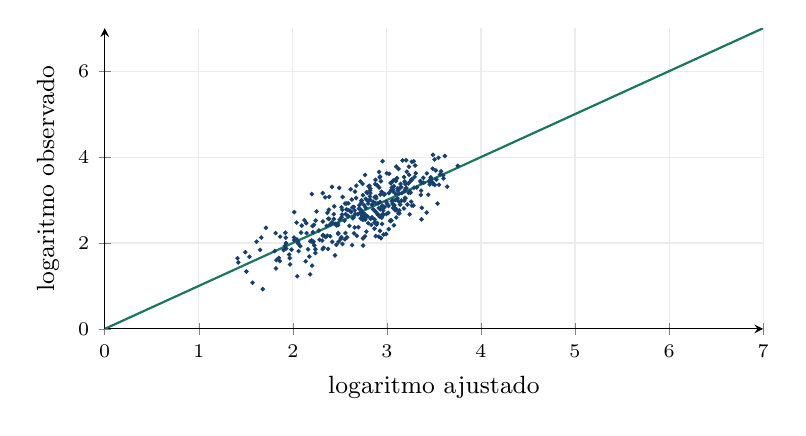
\begin{tikzpicture}\begin{axis}[base,width=.82\textwidth,height=5.4cm,xlabel={logaritmo ajustado},ylabel={logaritmo observado},xmin=0,xmax=7,ymin=0,ymax=7]
\addplot[only marks,mark=*,mark size=.6pt,azul] coordinates {(2.228179,1.942769) (3.363761,3.218755) (1.902226,1.834295) (1.851528,1.652199) (2.492918,3.282111) (1.928772,1.870241) (3.123489,3.724116) (3.288058,3.28712) (2.515761,2.13357) (3.284833,3.90289) (1.806466,1.811617) (2.770019,2.592681) (2.481417,2.21317) (3.035658,2.524618) (2.508914,2.095391) (3.017521,2.863755) (2.76966,2.544963) (2.954207,2.662927) (2.948988,2.8589) (1.816958,2.228926) (1.411492,1.644002) (2.927554,2.95601) (3.262473,3.480734) (3.21796,2.895579) (2.382651,2.773531) (2.740361,2.546797) (3.099301,3.776328) (3.155492,2.985559) (2.996077,2.676698) (2.927554,3.545553) (1.920326,2.237155) (2.283137,2.075446) (3.116364,3.219789) (2.325528,2.180936) (2.397171,2.157097) (2.358959,2.399096) (2.936459,3.435604) (3.538562,2.918049) (3.064539,2.995715) (2.916819,3.654799) (3.451372,3.438342) (2.975702,3.139131) (2.674585,3.33477) (3.574895,3.666977) (2.932356,2.787434) (3.211878,3.659897) (1.664401,2.12703) (2.773931,2.821655) (2.418759,2.025432) (3.519706,3.688703) (2.937158,2.113536) (2.961091,2.756745) (1.651922,1.839807) (2.663306,2.673637) (2.954553,2.668196) (2.047068,1.225675) (3.061037,2.908013) (3.079296,2.88064) (3.19738,3.36887) (2.39602,2.431174) (2.889437,2.428951) (2.964729,2.662406) (3.132594,2.688579) (2.161558,1.851378) (2.786006,2.998879) (3.509583,3.35129) (2.974583,2.838745) (3.486672,3.729464) (2.992209,2.96058) (2.224706,2.423004) (3.09477,3.443253) (1.925577,2.123504) (2.934867,2.621657) (3.248048,3.432293) (2.480766,2.413509) (2.079359,1.925449) (2.238852,1.853735) (2.526448,2.77189) (3.053306,2.971765) (2.742042,3.376721) (3.023998,3.610599) (2.946099,2.624915) (2.660552,3.195704) (2.276549,2.289717) (3.355645,3.443103) (3.281725,2.873026) (2.736026,2.634047) (1.505652,1.33597) (2.31806,3.161441) (2.758382,2.880164) (2.367479,2.701583) (3.021413,3.161679) (2.89621,2.467716) (1.494257,1.784915) (1.61408,2.030083) (2.656786,2.758673) (2.76462,2.673204) (1.825181,1.601285) (2.415841,3.305988) (2.783522,3.182211) (3.424745,3.620534) (3.001365,2.914508) (1.960628,1.729945) (3.364065,3.407615) (2.462418,1.959275) (2.991562,2.210236) (2.657811,2.36113) (1.860882,1.578945) (2.142656,2.461961) (2.626921,3.0095) (3.188284,3.205294) (2.384305,2.561072) (2.6386,2.574303) (2.183561,1.269905) (2.014931,2.06583) (2.448246,1.71164) (2.740065,2.609447) (2.585169,2.767276) (2.875799,3.37073) (2.83467,2.422028) (3.264325,3.889343) (3.257576,2.96156) (3.241602,2.665072) (2.213337,2.252292) (3.18968,3.418655) (1.985474,1.844191) (2.517437,2.832352) (2.136548,1.573173) (2.915456,2.146104) (2.18459,2.040356) (2.20124,3.138142) (2.014839,2.71712) (3.037102,2.511475) (2.482659,2.227943) (2.523393,2.660489) (2.374195,1.860119) (2.716009,2.701089) (2.727572,2.98128) (2.386283,3.074985) (1.967327,1.647719) (2.175169,1.683344) (2.930522,2.784517) (2.204481,1.471895) (2.316559,1.855876) (2.73172,2.991553) (3.038686,3.398789) (2.969956,3.1266) (3.525718,3.477123) (3.043706,3.226073) (3.262952,3.473506) (2.820028,3.08325) (2.804827,3.318242) (2.884198,3.082269) (2.878959,3.468437) (2.67988,2.166509) (2.553605,2.083943) (3.126311,3.145931) (2.011742,2.127802) (2.691371,2.668655) (3.019561,2.321965) (2.753815,2.683204) (3.367859,2.549437) (3.231275,3.167209) (2.450471,2.446373) (2.952597,2.868937) (3.104535,2.77666) (3.753274,3.797032) (3.391161,3.402945) (3.602186,3.502935) (2.745369,3.112512) (2.44016,2.853354) (2.607588,2.754511) (3.092553,3.475032) (3.048133,2.524605) (2.873148,2.744253) (2.1464,2.230181) (2.744775,2.541331) (3.065174,3.243327) (2.854113,2.783759) (2.518762,2.599721) (2.868051,2.332632) (2.570111,2.919841) (3.152732,3.301583) (2.794049,3.164525) (2.881243,2.72561) (3.121077,2.690734) (2.823545,3.1626) (3.5487,3.983644) (2.239602,1.765497) (2.706675,2.879753) (2.311878,2.056176) (3.265676,2.870233) (3.360495,3.118979) (2.486675,2.028714) (2.826254,2.5628) (2.81517,3.331276) (3.088047,2.999035) (2.319818,2.49999) (3.089689,3.148648) (3.489247,4.051796) (2.801066,2.918176) (3.192284,3.052714) (2.96733,2.821365) (2.9039,2.657671) (1.9137,1.929072) (1.927643,1.999152) (2.649078,2.840959) (2.998686,3.621522) (2.917563,3.290757) (3.386986,3.517072) (2.69772,2.367693) (3.065237,2.814289) (2.436207,2.557995) (2.56198,2.670714) (2.633062,2.828751) (2.327571,1.889052) (2.527074,1.97817) (2.559173,2.230343) (2.211874,2.013181) (2.88016,2.928318) (2.885231,3.0407) (1.538337,1.678464) (2.964572,2.197371) (2.057998,1.984697) (3.062818,3.202166) (1.820471,1.406628) (3.051762,3.290867) (2.122808,2.531391) (2.343109,3.062889) (2.822342,3.005936) (2.948175,2.443187) (2.718155,3.434065) (3.181251,2.804693) (3.068821,3.454729) (3.203953,3.926821) (2.086864,2.241325) (2.054421,2.028057) (2.924904,3.526057) (2.600471,2.398423) (2.37667,2.563549) (3.295048,3.539388) (1.679687,0.9258381) (2.944142,3.193227) (2.619505,2.718157) (2.589839,2.923962) (2.19957,2.056124) (2.476157,2.446313) (3.484441,3.410362) (2.721495,2.570855) (1.71345,2.353496) (2.801286,2.985769) (3.23602,3.587065) (1.865002,2.148175) (2.555371,2.917999) (3.56435,3.593821) (2.944068,2.588584) (3.317526,3.292826) (3.113384,3.269851) (3.243037,3.200147) (2.869745,2.548671) (2.841785,2.596109) (3.107205,3.510266) (2.730258,2.941672) (3.131648,2.757195) (3.07361,3.320839) (3.234785,3.77603) (2.880906,2.160697) (2.416376,2.479258) (3.455808,3.433554) (3.37111,2.818189) (3.140159,2.89522) (2.740075,2.714688) (2.251715,2.734752) (2.094718,2.403185) (3.184751,2.98364) (2.926274,2.282459) (2.841542,2.886604) (2.497182,2.544645) (3.18825,3.43383) (2.650999,2.224297) (3.112439,3.040623) (2.855146,2.959083) (3.195935,3.252459) (1.969898,1.499824) (3.439353,3.122895) (2.435329,2.669236) (2.901655,2.676716) (3.61634,4.025421) (3.089285,2.762568) (2.968982,3.129048) (2.869343,3.068065) (2.954193,3.904564) (3.466046,3.480927) (2.92537,2.606959) (2.528958,3.070373) (3.299751,3.803866) (2.702414,2.801645) (2.366353,2.168675) (3.079826,2.825792) (2.209466,2.394122) (3.229039,3.387586) (2.6726,3.048107) (3.506717,3.946038) (3.074417,2.411852) (3.182296,3.535884) (2.899629,3.337214) (3.490346,3.376547) (2.906017,2.922982) (3.119581,3.225896) (2.317254,2.173959) (3.455186,3.362585) (3.465505,3.527806) (2.569391,2.782362) (2.820949,3.224648) (3.099277,2.593711) (3.250562,3.171441) (2.34811,2.139348) (3.266774,3.481826) (2.061142,1.80951) (3.465921,3.485141) (2.747452,1.940662) (3.207314,3.281511) (1.42019,1.546391) (3.422818,2.707704) (3.553871,3.354976) (2.86918,2.475236) (2.646884,2.602356) (2.822649,3.265438) (2.746227,2.107399) (3.597083,3.575776) (2.585478,2.632378) (3.305941,3.624935) (2.463592,2.409389) (2.72126,2.780693) (2.766655,2.154599) (2.914191,2.812816) (3.014744,2.701207) (2.548436,2.519856) (2.800766,2.461701) (2.767327,3.58442) (3.124647,2.972092) (3.196431,3.041572) (2.242399,2.521714) (3.166572,3.922274) (2.220384,2.030919) (2.042454,2.081548) (2.931084,3.128428) (2.576478,2.131069) (3.047132,3.398232) (2.793909,2.621385) (2.629999,1.949787) (2.039984,2.474167) (3.640554,3.311225) (1.571434,1.074486) (2.775392,3.02991) (3.145319,3.375261) (3.140095,3.285679) (2.614765,3.250362) (3.1604,3.162535) (2.781542,2.264954)};
\addplot[verde,thick,domain=0:7]{x};
\end{axis}\end{tikzpicture}\caption{Logaritmos artificiales observados y ajustados con el diseño Mincer.}\end{figure}

Ambos ajustes usan las mismas 360 personas. Mincer conserva su bloque de controles y calendario; el principal añade los cinco términos digitales y de informalidad. La diagonal representa coincidencia entre resultado y ajuste.

La dispersión vertical de cada persona es su residuo. Una figura de ajuste no demuestra la condición de media cero del error poblacional. Un $R^2$ alto tampoco valida exclusiones de selección.

\clearpage
\section{Resultado y ajuste del modelo principal en las mismas personas}
\begin{figure}[H]\centering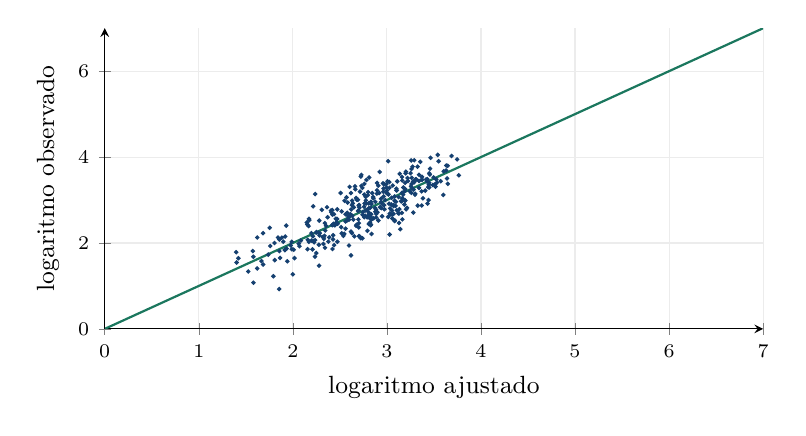
\begin{tikzpicture}\begin{axis}[base,width=.82\textwidth,height=5.4cm,xlabel={logaritmo ajustado},ylabel={logaritmo observado},xmin=0,xmax=7,ymin=0,ymax=7]
\addplot[only marks,mark=*,mark size=.6pt,azul] coordinates {(1.976807,1.942769) (3.407655,3.218755) (1.91434,1.834295) (1.864217,1.652199) (2.738975,3.282111) (1.932787,1.870241) (3.261876,3.724116) (3.265902,3.28712) (2.325613,2.13357) (3.550039,3.90289) (1.57426,1.811617) (2.832867,2.592681) (2.546546,2.21317) (2.909272,2.524618) (2.329769,2.095391) (3.092159,2.863755) (2.83474,2.544963) (3.040471,2.662927) (3.071394,2.8589) (1.683376,2.228926) (1.421227,1.644002) (2.937723,2.95601) (3.311424,3.480734) (3.047094,2.895579) (2.791817,2.773531) (2.586353,2.546797) (3.325798,3.776328) (3.195592,2.985559) (3.070159,2.676698) (2.72274,3.545553) (2.271217,2.237155) (2.158747,2.075446) (3.000009,3.219789) (2.428304,2.180936) (2.212726,2.157097) (2.353556,2.399096) (3.007198,3.435604) (3.431964,2.918049) (3.19122,2.995715) (2.923197,3.654799) (3.571995,3.438342) (3.013195,3.139131) (2.908602,3.33477) (3.60432,3.666977) (3.132602,2.787434) (3.202728,3.659897) (1.621254,2.12703) (2.707473,2.821655) (2.169986,2.025432) (3.630847,3.688703) (2.72148,2.113536) (2.776675,2.756745) (1.915984,1.839807) (2.822525,2.673637) (2.832685,2.668196) (1.792944,1.225675) (2.836156,2.908013) (3.072616,2.88064) (2.993255,3.36887) (2.154368,2.431174) (2.829465,2.428951) (2.806822,2.662406) (3.128448,2.688579) (2.209354,1.851378) (2.981219,2.998879) (3.487529,3.35129) (2.930562,2.838745) (3.458498,3.729464) (2.830656,2.96058) (2.425397,2.423004) (3.340645,3.443253) (1.882264,2.123504) (2.94891,2.621657) (3.279042,3.432293) (2.41821,2.413509) (2.069558,1.925449) (1.989323,1.853735) (2.30787,2.77189) (3.151254,2.971765) (2.760214,3.376721) (3.136084,3.610599) (2.802881,2.624915) (2.713728,3.195704) (2.344244,2.289717) (3.223195,3.443103) (3.370486,2.873026) (2.767735,2.634047) (1.525957,1.33597) (2.617706,3.161441) (2.628468,2.880164) (2.578896,2.701583) (2.844334,3.161679) (3.12924,2.467716) (1.397463,1.784915) (1.898006,2.030083) (2.699365,2.758673) (2.57402,2.673204) (1.807835,1.601285) (2.603947,3.305988) (2.79934,3.182211) (3.450905,3.620534) (3.022465,2.914508) (1.738266,1.729945) (3.531877,3.407615) (2.276896,1.959275) (2.836455,2.210236) (2.700794,2.36113) (1.666232,1.578945) (2.340631,2.461961) (2.679084,3.0095) (3.243781,3.205294) (2.170972,2.561072) (2.859643,2.574303) (1.99948,1.269905) (2.23615,2.06583) (2.617915,1.71164) (2.590995,2.609447) (2.41954,2.767276) (2.969319,3.37073) (2.677015,2.422028) (3.354999,3.889343) (3.096414,2.96156) (3.053182,2.665072) (2.251153,2.252292) (3.025647,3.418655) (2.008702,1.844191) (2.363035,2.832352) (1.941142,1.573173) (2.711897,2.146104) (2.21895,2.040356) (2.237212,3.138142) (2.408954,2.71712) (3.082378,2.511475) (2.285847,2.227943) (2.420615,2.660489) (2.421816,1.860119) (2.808895,2.701089) (2.549566,2.98128) (2.773002,3.074985) (2.017813,1.647719) (2.235463,1.683344) (2.973678,2.784517) (2.278834,1.471895) (2.156026,1.855876) (2.776445,2.991553) (2.895286,3.398789) (3.172188,3.1266) (3.416808,3.477123) (2.895548,3.226073) (3.37271,3.473506) (2.964147,3.08325) (2.661076,3.318242) (3.082519,3.082269) (2.782401,3.468437) (2.537142,2.166509) (2.426676,2.083943) (3.300798,3.145931) (1.842159,2.127802) (2.560668,2.668655) (3.14246,2.321965) (3.03002,2.683204) (3.163913,2.549437) (3.259527,3.167209) (2.431039,2.446373) (2.7005,2.868937) (2.884279,2.77666) (3.646374,3.797032) (3.449188,3.402945) (3.639425,3.502935) (2.796892,3.112512) (2.215562,2.853354) (2.405263,2.754511) (3.372516,3.475032) (3.083849,2.524605) (2.693847,2.744253) (2.196724,2.230181) (2.597507,2.541331) (3.283972,3.243327) (3.204175,2.783759) (2.369392,2.599721) (2.56012,2.332632) (2.806363,2.919841) (3.438256,3.301583) (2.50779,3.164525) (2.876393,2.72561) (3.1217,2.690734) (2.918257,3.1626) (3.464004,3.983644) (2.249242,1.765497) (2.969661,2.879753) (2.084559,2.056176) (3.328089,2.870233) (3.599936,3.118979) (2.473129,2.028714) (2.843484,2.5628) (2.729538,3.331276) (3.442796,2.999035) (2.559525,2.49999) (2.8929,3.148648) (3.540311,4.051796) (2.780488,2.918176) (3.050669,3.052714) (2.823329,2.821365) (2.741152,2.657671) (1.759999,1.929072) (1.80436,1.999152) (2.757145,2.840959) (3.198257,3.621522) (2.99516,3.290757) (3.263761,3.517072) (2.513483,2.367693) (2.874802,2.814289) (2.471094,2.557995) (2.610901,2.670714) (2.649152,2.828751) (2.341653,1.889052) (2.324777,1.97817) (2.628333,2.230343) (2.226352,2.013181) (2.945148,2.928318) (2.856848,3.0407) (1.580192,1.678464) (3.028809,2.197371) (2.062,1.984697) (3.188804,3.202166) (1.620861,1.406628) (3.449769,3.290867) (2.175216,2.531391) (2.570275,3.062889) (2.692113,3.005936) (2.807406,2.443187) (3.10961,3.434065) (3.034193,2.804693) (3.162756,3.454729) (3.290556,3.926821) (2.247982,2.241325) (1.987732,2.028057) (2.811145,3.526057) (2.672356,2.398423) (2.457193,2.563549) (3.372597,3.539388) (1.854575,0.9258381) (2.961785,3.193227) (2.743945,2.718157) (2.637344,2.923962) (2.199471,2.056124) (2.476802,2.446313) (3.28767,3.410362) (3.057867,2.570855) (1.7535,2.353496) (2.630283,2.985769) (3.341407,3.587065) (1.918519,2.148175) (2.766958,2.917999) (3.45594,3.593821) (2.811458,2.588584) (3.175063,3.292826) (2.96398,3.269851) (3.369111,3.200147) (2.696547,2.548671) (2.790269,2.596109) (3.219503,3.510266) (2.582921,2.941672) (3.052659,2.757195) (3.256468,3.320839) (3.272872,3.77603) (2.703014,2.160697) (2.462927,2.479258) (3.426635,3.433554) (3.213693,2.818189) (3.185853,2.89522) (2.899268,2.714688) (2.519073,2.734752) (1.9296,2.403185) (3.081671,2.98364) (2.792766,2.282459) (2.703976,2.886604) (2.643159,2.544645) (3.290933,3.43383) (2.519523,2.224297) (3.382923,3.040623) (2.876736,2.959083) (3.196273,3.252459) (1.683674,1.499824) (3.298653,3.122895) (2.437035,2.669236) (2.886472,2.676716) (3.687328,4.025421) (3.10485,2.762568) (3.016387,3.129048) (3.125374,3.068065) (3.013615,3.904564) (3.524549,3.480927) (3.013349,2.606959) (2.853946,3.070373) (3.630573,3.803866) (2.805578,2.801645) (2.336399,2.168675) (2.929354,2.825792) (2.167124,2.394122) (2.958646,3.387586) (2.672246,3.048107) (3.746335,3.946038) (2.826247,2.411852) (3.160781,3.535884) (3.062225,3.337214) (3.647413,3.376547) (2.763519,2.922982) (3.105557,3.225896) (2.283054,2.173959) (3.510686,3.362585) (3.496629,3.527806) (2.472162,2.782362) (3.100622,3.224648) (2.886746,2.593711) (3.161408,3.171441) (2.319209,2.139348) (3.304989,3.481826) (1.856823,1.80951) (3.428969,3.485141) (2.596822,1.940662) (3.34119,3.281511) (1.402312,1.546391) (3.280765,2.707704) (3.446245,3.354976) (2.819221,2.475236) (2.758941,2.602356) (3.100066,3.265438) (2.739769,2.107399) (3.764458,3.575776) (2.632438,2.632378) (3.252065,3.624935) (2.447135,2.409389) (2.620226,2.780693) (2.653486,2.154599) (2.941644,2.812816) (3.159083,2.701207) (2.573888,2.519856) (2.70137,2.461701) (2.728361,3.58442) (3.156586,2.972092) (3.164345,3.041572) (2.280525,2.521714) (3.257868,3.922274) (2.377603,2.030919) (1.857036,2.081548) (2.759043,3.128428) (2.386165,2.131069) (3.19369,3.398232) (2.602637,2.621385) (2.439237,1.949787) (2.148545,2.474167) (3.517637,3.311225) (1.5812,1.074486) (2.937667,3.02991) (3.261994,3.375261) (3.026904,3.285679) (2.664161,3.250362) (2.995567,3.162535) (2.618148,2.264954)};
\addplot[verde,thick,domain=0:7]{x};
\end{axis}\end{tikzpicture}\caption{Logaritmos artificiales observados y ajustados con el diseño principal.}\end{figure}

Ambos ajustes usan las mismas 360 personas. Mincer conserva su bloque de controles y calendario; el principal añade los cinco términos digitales y de informalidad. La diagonal representa coincidencia entre resultado y ajuste.

La dispersión vertical de cada persona es su residuo. Una figura de ajuste no demuestra la condición de media cero del error poblacional. Un $R^2$ alto tampoco valida exclusiones de selección.

\clearpage
\section{Problema de selección normal con argumento -3}

\[
\frac{\phi(-3)}{\Phi(-3)}=3.283098655,\quad
\left(\frac{\phi}{\Phi}\right)'(-3)=-0.9294408132.
\]

\[
\E[\nu_i\mid S_i=1]=3.283098655,\quad
\Var(\nu_i\mid S_i=1)=0.07055918679.
\]

\[
\E[\varepsilon_i^{(0)}\mid S_i=1]=.175(3.283098655)=0.5745422646,
\]

\[
\Var(\varepsilon_i^{(0)}\mid S_i=1)=.35^2[1+.5^2(-0.9294408132)]=0.0940358751.
\]

El argumento escalar representa una realización de la suma completa $Z_i^{\mathsf T}\pi+\lambda_{y(i)}^{(S)}+\mu_{m(i)}^{(S)}$. No reemplaza regresores del modelo por una variable inventada.

La probabilidad corresponde al área normal por encima del umbral negativo. El resultado seleccionado del error se obtiene con la misma truncación, no con una distribución normal ordinaria de igual media.
\begin{figure}[H]\centering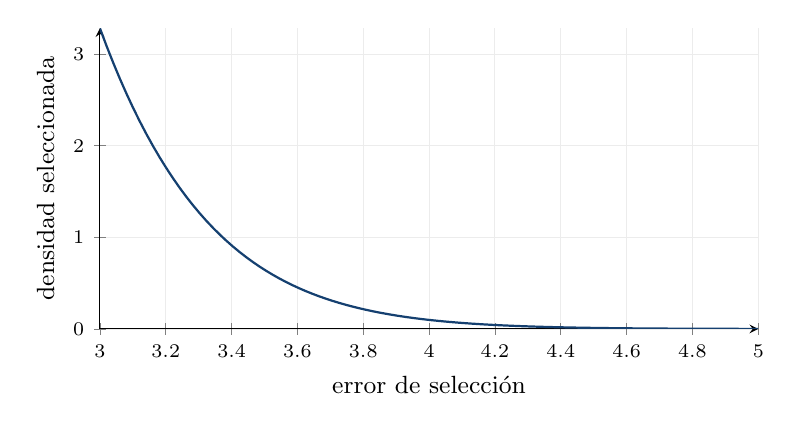
\begin{tikzpicture}\begin{axis}[base,width=.82\textwidth,height=5.4cm,xlabel={error de selección},ylabel={densidad seleccionada},xmin=3,xmax=5]
\addplot[azul,thick,domain=3:5]{exp(-x*x/2)/sqrt(2*pi)/0.0013498980316300933};
\end{axis}\end{tikzpicture}\caption{Densidad de selección truncada para el argumento -3.}\end{figure}

\clearpage
\section{Problema de selección normal con argumento -1}

\[
\frac{\phi(-1)}{\Phi(-1)}=1.525135276,\quad
\left(\frac{\phi}{\Phi}\right)'(-1)=-0.8009023344.
\]

\[
\E[\nu_i\mid S_i=1]=1.525135276,\quad
\Var(\nu_i\mid S_i=1)=0.1990976656.
\]

\[
\E[\varepsilon_i^{(0)}\mid S_i=1]=.175(1.525135276)=0.2668986733,
\]

\[
\Var(\varepsilon_i^{(0)}\mid S_i=1)=.35^2[1+.5^2(-0.8009023344)]=0.09797236601.
\]

El argumento escalar representa una realización de la suma completa $Z_i^{\mathsf T}\pi+\lambda_{y(i)}^{(S)}+\mu_{m(i)}^{(S)}$. No reemplaza regresores del modelo por una variable inventada.

La probabilidad corresponde al área normal por encima del umbral negativo. El resultado seleccionado del error se obtiene con la misma truncación, no con una distribución normal ordinaria de igual media.
\begin{figure}[H]\centering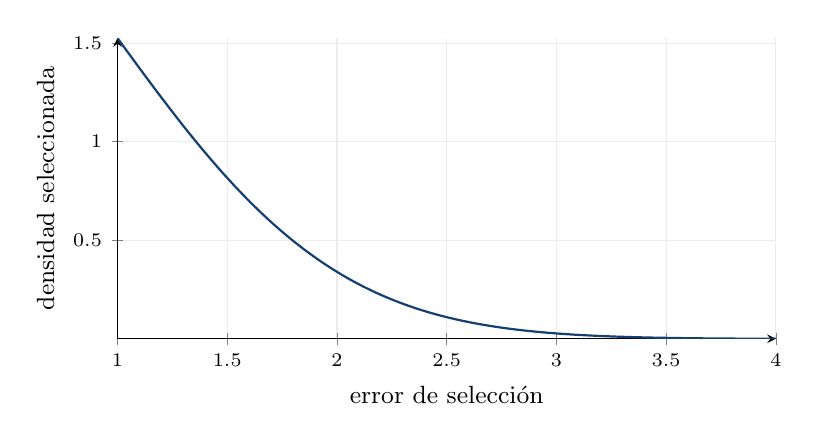
\begin{tikzpicture}\begin{axis}[base,width=.82\textwidth,height=5.4cm,xlabel={error de selección},ylabel={densidad seleccionada},xmin=1,xmax=4]
\addplot[azul,thick,domain=1:4]{exp(-x*x/2)/sqrt(2*pi)/0.15865525393145707};
\end{axis}\end{tikzpicture}\caption{Densidad de selección truncada para el argumento -1.}\end{figure}

\clearpage
\section{Problema de selección normal con argumento 0}

\[
\frac{\phi(0)}{\Phi(0)}=0.7978845608,\quad
\left(\frac{\phi}{\Phi}\right)'(0)=-0.6366197724.
\]

\[
\E[\nu_i\mid S_i=1]=0.7978845608,\quad
\Var(\nu_i\mid S_i=1)=0.3633802276.
\]

\[
\E[\varepsilon_i^{(0)}\mid S_i=1]=.175(0.7978845608)=0.1396297981,
\]

\[
\Var(\varepsilon_i^{(0)}\mid S_i=1)=.35^2[1+.5^2(-0.6366197724)]=0.1030035195.
\]

El argumento escalar representa una realización de la suma completa $Z_i^{\mathsf T}\pi+\lambda_{y(i)}^{(S)}+\mu_{m(i)}^{(S)}$. No reemplaza regresores del modelo por una variable inventada.

La probabilidad corresponde al área normal por encima del umbral negativo. El resultado seleccionado del error se obtiene con la misma truncación, no con una distribución normal ordinaria de igual media.
\begin{figure}[H]\centering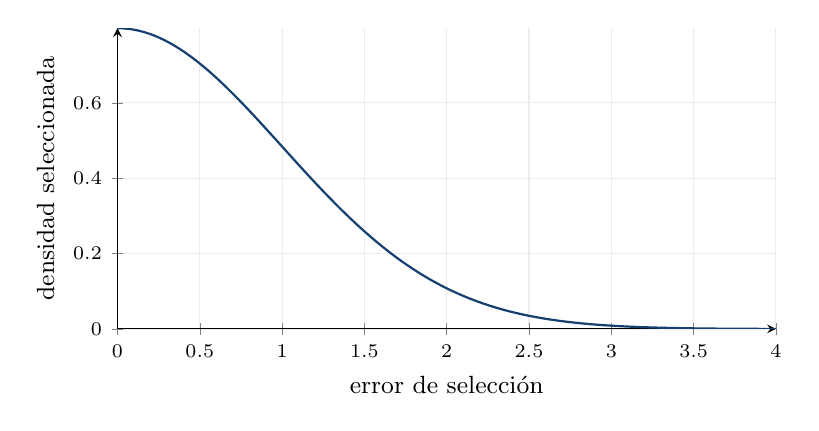
\begin{tikzpicture}\begin{axis}[base,width=.82\textwidth,height=5.4cm,xlabel={error de selección},ylabel={densidad seleccionada},xmin=0,xmax=4]
\addplot[azul,thick,domain=0:4]{exp(-x*x/2)/sqrt(2*pi)/0.5};
\end{axis}\end{tikzpicture}\caption{Densidad de selección truncada para el argumento 0.}\end{figure}

\clearpage
\section{Problema de selección normal con argumento 1}

\[
\frac{\phi(1)}{\Phi(1)}=0.2875999709,\quad
\left(\frac{\phi}{\Phi}\right)'(1)=-0.3703137142.
\]

\[
\E[\nu_i\mid S_i=1]=0.2875999709,\quad
\Var(\nu_i\mid S_i=1)=0.6296862858.
\]

\[
\E[\varepsilon_i^{(0)}\mid S_i=1]=.175(0.2875999709)=0.05032999491,
\]

\[
\Var(\varepsilon_i^{(0)}\mid S_i=1)=.35^2[1+.5^2(-0.3703137142)]=0.1111591425.
\]

El argumento escalar representa una realización de la suma completa $Z_i^{\mathsf T}\pi+\lambda_{y(i)}^{(S)}+\mu_{m(i)}^{(S)}$. No reemplaza regresores del modelo por una variable inventada.

La probabilidad corresponde al área normal por encima del umbral negativo. El resultado seleccionado del error se obtiene con la misma truncación, no con una distribución normal ordinaria de igual media.
\begin{figure}[H]\centering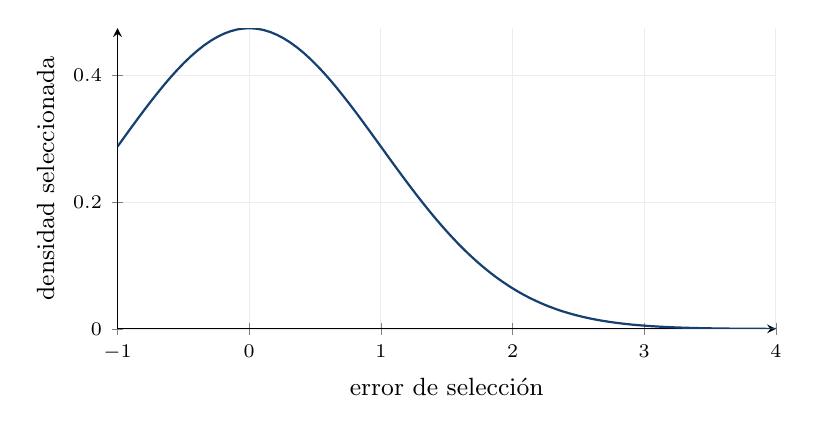
\begin{tikzpicture}\begin{axis}[base,width=.82\textwidth,height=5.4cm,xlabel={error de selección},ylabel={densidad seleccionada},xmin=-1,xmax=4]
\addplot[azul,thick,domain=-1:4]{exp(-x*x/2)/sqrt(2*pi)/0.8413447460685429};
\end{axis}\end{tikzpicture}\caption{Densidad de selección truncada para el argumento 1.}\end{figure}

\clearpage
\section{Problema de selección normal con argumento 3}

\[
\frac{\phi(3)}{\Phi(3)}=0.004437839042,\quad
\left(\frac{\phi}{\Phi}\right)'(3)=-0.01333321154.
\]

\[
\E[\nu_i\mid S_i=1]=0.004437839042,\quad
\Var(\nu_i\mid S_i=1)=0.9866667885.
\]

\[
\E[\varepsilon_i^{(0)}\mid S_i=1]=.175(0.004437839042)=0.0007766218324,
\]

\[
\Var(\varepsilon_i^{(0)}\mid S_i=1)=.35^2[1+.5^2(-0.01333321154)]=0.1220916704.
\]

El argumento escalar representa una realización de la suma completa $Z_i^{\mathsf T}\pi+\lambda_{y(i)}^{(S)}+\mu_{m(i)}^{(S)}$. No reemplaza regresores del modelo por una variable inventada.

La probabilidad corresponde al área normal por encima del umbral negativo. El resultado seleccionado del error se obtiene con la misma truncación, no con una distribución normal ordinaria de igual media.
\begin{figure}[H]\centering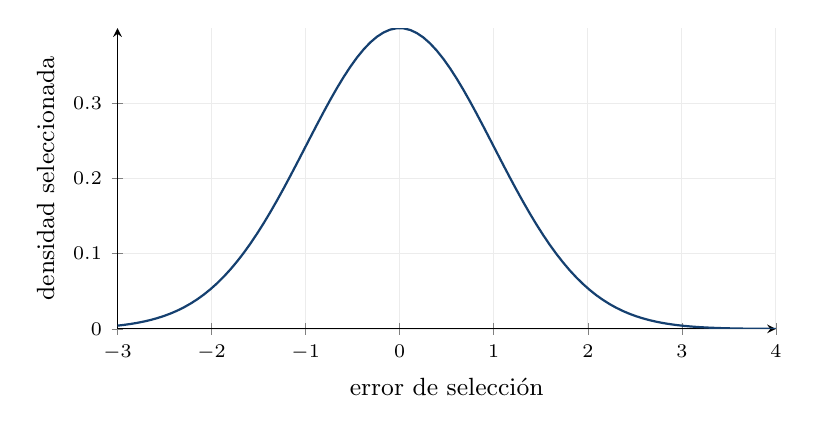
\begin{tikzpicture}\begin{axis}[base,width=.82\textwidth,height=5.4cm,xlabel={error de selección},ylabel={densidad seleccionada},xmin=-3,xmax=4]
\addplot[azul,thick,domain=-3:4]{exp(-x*x/2)/sqrt(2*pi)/0.9986501019683699};
\end{axis}\end{tikzpicture}\caption{Densidad de selección truncada para el argumento 3.}\end{figure}

\clearpage
\phantomsection\addcontentsline{toc}{subsection}{Aplicaciones adicionales a la tesis y límites que la matemática exige}
{\large\bfseries\color{azul}Aplicaciones adicionales a la tesis y límites que la matemática exige}\par\vspace{2mm}
\section{Derivar experiencia cuando aparece en más de una columna salarial y de selección}

La experiencia original aparece en $x_{i1,2}$ y en su cuadrado $x_{i1,3}$. Por cadena, la derivada de la media salarial sin selección es
$\gamma_{1,2}+2\gamma_{1,3}\operatorname{Experiencia}_i$.

Si el contenido justificado de $Z_i$ incluye también experiencia y su cuadrado, la derivada de su argumento es
$\pi_{\rm experiencia}+2\pi_{\rm experiencia^2}\operatorname{Experiencia}_i$.
No se asigna ese contenido como definitivo: la ecuación de selección original no enumera sus entradas.
\[
\begin{aligned}
\frac{\partial\E[w_i\mid W_i,Z_i,S_i=1]}
{\partial\operatorname{Experiencia}_i}
={}&\gamma_{1,2}+2\gamma_{1,3}\operatorname{Experiencia}_i\\
&-\kappa\frac{\phi(Z_i^{\mathsf T}\pi+\lambda_{y(i)}^{(S)}+\mu_{m(i)}^{(S)})}
{\Phi(Z_i^{\mathsf T}\pi+\lambda_{y(i)}^{(S)}+\mu_{m(i)}^{(S)})}\\
&\cdot\left[Z_i^{\mathsf T}\pi+\lambda_{y(i)}^{(S)}+\mu_{m(i)}^{(S)}
+\frac{\phi(Z_i^{\mathsf T}\pi+\lambda_{y(i)}^{(S)}+\mu_{m(i)}^{(S)})}
{\Phi(Z_i^{\mathsf T}\pi+\lambda_{y(i)}^{(S)}+\mu_{m(i)}^{(S)})}\right]\\
&\cdot(\pi_{\rm experiencia}+2\pi_{\rm experiencia^2}\operatorname{Experiencia}_i).
\end{aligned}
\]
La derivada de una columna del diseño no equivale siempre a la derivada de una característica original que genera varias columnas. El mismo cuidado se aplica al conteo, al centrado y a sus interacciones.

\clearpage
\section{Uso digital binario y comparación seleccionada de perfiles admisibles}

El paso de no usuario a usuario no se obtiene derivando $U_i$ manteniendo un conteo incompatible con $U_i=0$. La comparación fija una intensidad admisible $t$ para el usuario y cero para el no usuario.

Entre formales, la diferencia salarial potencial literal es $\beta_u+t\beta_a$. La diferencia entre medias seleccionadas añade
\[
\kappa\left[
\frac{\phi(Z_i^{(U=1,A=t)\mathsf T}\pi+\lambda_{y(i)}^{(S)}+\mu_{m(i)}^{(S)})}
{\Phi(Z_i^{(U=1,A=t)\mathsf T}\pi+\lambda_{y(i)}^{(S)}+\mu_{m(i)}^{(S)})}
-
\frac{\phi(Z_i^{(U=0,A=0)\mathsf T}\pi+\lambda_{y(i)}^{(S)}+\mu_{m(i)}^{(S)})}
{\Phi(Z_i^{(U=0,A=0)\mathsf T}\pi+\lambda_{y(i)}^{(S)}+\mu_{m(i)}^{(S)})}
\right].
\]
Los superíndices indican escenarios de los regresores existentes. Si $Z_i$ no contiene una función del uso o actividades y los demás condicionantes son idénticos, el término adicional se cancela.

Entre informales la parte salarial potencial es
$\beta_u+t\beta_a+\delta_u+(t-\overline A_u)\delta_a$.
Los errores estándar deben propagarse respecto de ambas ecuaciones cuando sus argumentos de selección cambian.

Ni el contraste potencial ni el seleccionado se convierte automáticamente en un efecto causal de adquirir tecnología. La hipótesis que identifica selección salarial es diferente de una hipótesis que identifica adopción exógena de TIC.

\clearpage
\section{Esperanza del ingreso en niveles bajo selección normal}

La media aritmética salarial seleccionada requiere integrar una exponencial del error, no exponentiar simplemente la media seleccionada de logaritmos.

Para un argumento escalar normal $t$, la descomposición
$\varepsilon^{(0)}=\rho\sigma\nu+\sigma\sqrt{1-\rho^2}u$
da
\[
\begin{aligned}
\E[e^{\varepsilon^{(0)}}\mid\nu>-t]
&=e^{\sigma^2(1-\rho^2)/2}
\frac{\int_{-t}^{\infty}e^{\rho\sigma v}\phi(v)\,\mathrm dv}{\Phi(t)}\\
&=e^{\sigma^2/2}\frac{\Phi(t+\rho\sigma)}{\Phi(t)}.
\end{aligned}
\]
En el último paso se completó el cuadrado:
$e^{\rho\sigma v}\phi(v)=e^{(\rho\sigma)^2/2}\phi(v-\rho\sigma)$.

Reemplazar el argumento por la suma de la ecuación de selección produce
\[
\E[y_i\mid W_i,Z_i,S_i=1]
=\exp\left(\sum_jW_{ij}\beta_j+\frac{\sigma^2}{2}\right)
\frac{\Phi(Z_i^{\mathsf T}\pi+\lambda_{y(i)}^{(S)}+\mu_{m(i)}^{(S)}+\rho\sigma)}
{\Phi(Z_i^{\mathsf T}\pi+\lambda_{y(i)}^{(S)}+\mu_{m(i)}^{(S)})}.
\]
La fórmula incluye la misma media principal completa. Es distinta de
$\exp(W_i^{\mathsf T}\beta+\kappa\lambda_i)$ porque la exponencial y la esperanza no conmutan.

\clearpage
\section{Segundo momento y varianza del ingreso seleccionado en soles}

La misma integración con $2\varepsilon^{(0)}$ da
\[
\E[e^{2\varepsilon_i^{(0)}}\mid S_i=1]
=e^{2\sigma^2}
\frac{\Phi(Z_i^{\mathsf T}\pi+\lambda_{y(i)}^{(S)}+\mu_{m(i)}^{(S)}+2\rho\sigma)}
{\Phi(Z_i^{\mathsf T}\pi+\lambda_{y(i)}^{(S)}+\mu_{m(i)}^{(S)})}.
\]
Multiplicar por la exponencial de dos veces la media salarial y restar el cuadrado del primer momento obtiene
\[
\begin{aligned}
\Var(y_i\mid W_i,Z_i,S_i=1)
={}&e^{2\sum_jW_{ij}\beta_j+2\sigma^2}
\frac{\Phi(Z_i^{\mathsf T}\pi+\lambda_{y(i)}^{(S)}+\mu_{m(i)}^{(S)}+2\rho\sigma)}
{\Phi(Z_i^{\mathsf T}\pi+\lambda_{y(i)}^{(S)}+\mu_{m(i)}^{(S)})}\\
&-e^{2\sum_jW_{ij}\beta_j+\sigma^2}
\left[
\frac{\Phi(Z_i^{\mathsf T}\pi+\lambda_{y(i)}^{(S)}+\mu_{m(i)}^{(S)}+\rho\sigma)}
{\Phi(Z_i^{\mathsf T}\pi+\lambda_{y(i)}^{(S)}+\mu_{m(i)}^{(S)})}
\right]^2.
\end{aligned}
\]
Los momentos en logaritmos y en soles pertenecen a objetos diferentes. La varianza en soles depende de la media salarial y no se obtiene exponenciando la varianza en logaritmos.

Bajo $\rho=0$ la razón de acumuladas es uno y se recupera la varianza lognormal ordinaria. Este límite comprueba la coherencia de la fórmula seleccionada.

\clearpage
\section{Efectos de año y mes como proyección y la cautela con el doble centrado}

Si se eliminara solo un conjunto de interceptos de grupo, restar el promedio de cada grupo de resultado y regresores reproduce su proyección. Con año y mes simultáneos, la eliminación general usa el producto cruzado conjunto de sus dummies.

En un diseño balanceado con pesos iguales, ciertos dobles centrados pueden coincidir con esa proyección. En una encuesta con celdas desiguales no se garantiza que
$w_i-\overline w_{y(i)}-\overline w_{m(i)}+\overline w$
sea el residuo exacto de la regresión sobre ambos bloques.

La proyección exacta usa la matriz de todas las dummies identificadas:
\[
I-D(D^{\mathsf T}D)^{-1}D^{\mathsf T}.
\]
Sus entradas de año--mes son conteos de las celdas. Si los tamaños cambian, también cambian los pesos de la proyección.

No se transforman datos mediante una regla de centrado incompleta para después afirmar equivalencia con las ecuaciones de la tesis. La regresión completa con dummies o una residualización exacta conservan el mismo ajuste.

La letra $D$ identifica aquí la matriz de dummies existentes, no una nueva variable explicativa ni un alias del resultado de una suma. Su producto cruzado se interpreta mediante esos conteos.

\clearpage
\section{Eliminar personas repetidas y cambiar el objetivo de la muestra}

La tesis indica que se retiran repeticiones entre años. Esa decisión altera el conjunto de personas y puede cambiar sus momentos:
\[
\frac1n\sum_iW_iW_i^{\mathsf T},\qquad
\frac1n\sum_iW_iw_i.
\]
No es únicamente un ajuste de errores estándar. Si una persona se conserva en 2023 y se excluye en 2024, cambian las composiciones anuales y las comparaciones pooled.

La correlación individual se relaciona con observaciones repetidas, pero la selección de qué repetición conservar requiere una regla. La matemática no demuestra que retirarlas produzca una muestra representativa ni independencia entre hogares.

Conservar una observación por persona permite estudiar un conjunto sin repeticiones personales. Las dummies de año siguen siendo efectos agregados de cortes agrupados, no interceptos fijos individuales.

En una base con identificadores únicos, un sándwich agrupado por persona tiene suma central de grupos unitarios. Si se desea considerar dependencia de la encuesta, deben examinarse hogar, conglomerado y diseño de muestreo.

El tratamiento de repeticiones debe aplicarse de forma coherente al definir la población del probit y la muestra salarial, sin eliminar automáticamente todos los no observables al reconstruir selección.

\clearpage
\section{Winsorización por año y el cambio matemático de variable dependiente}

El documento propone sustituir por el percentil uno y noventa y nueve de cada año los ingresos fuera de sus límites. Si los límites son $c_{.01,y}$ y $c_{.99,y}$, el ingreso ajustado es
\[
y_i^{\rm ajustado}=
\min\left\{\max\{y_i,c_{.01,y(i)}\},c_{.99,y(i)}\right\}.
\]
El logaritmo ajustado utiliza esa cantidad, no el residuo de la regresión. Como el logaritmo es monótono,
\[
\ln(y_i^{\rm ajustado})
=\min\{\max\{\ln(y_i),\ln(c_{.01,y(i)})\},\ln(c_{.99,y(i)})\}.
\]
Con diseño y muestra fijos, el cambio de coeficientes es exactamente
\[
\widehat\beta_{\rm ajustado}-\widehat\beta
=[\sum_iW_iW_i^{\mathsf T}]^{-1}
\sum_iW_i[\ln(y_i^{\rm ajustado})-\ln(y_i)].
\]
No se eliminan observaciones por esta operación. La identidad permite ver qué características se correlacionan con las modificaciones de cola.

Los límites estimados son también aleatorios. Una inferencia que repite el procedimiento completo en un remuestreo vuelve a estimarlos por año. La prueba con ingreso ajustado se identifica como sensibilidad de la dependiente; no es automáticamente una corrección de selección.

\clearpage
\section{Horas, logaritmos y la incertidumbre de una medición de ingreso}

Para pequeñas perturbaciones de las fuentes del ingreso horario, el diferencial es
\[
\mathrm dw_i=
\frac{\mathrm d\operatorname{IngresoAnual}_i}{\operatorname{IngresoAnual}_i}
-\frac{\mathrm d\operatorname{I513T}_i}{\operatorname{I513T}_i}.
\]
La varianza aproximada de un error de medición de $w_i$, manteniendo fijos los denominadores, incluye
\[
\begin{aligned}
&\frac{\Var(\mathrm d\operatorname{IngresoAnual}_i)}
{\operatorname{IngresoAnual}_i^2}
+\frac{\Var(\mathrm d\operatorname{I513T}_i)}
{\operatorname{I513T}_i^2}\\
&\quad-
\frac{2\Cov(\mathrm d\operatorname{IngresoAnual}_i,
\mathrm d\operatorname{I513T}_i)}
{\operatorname{IngresoAnual}_i\operatorname{I513T}_i}.
\end{aligned}
\]
Los errores de ambas respuestas pueden estar relacionados. La transformación logarítmica no vuelve independientes sus fuentes.

Un error en la dependiente con media condicional cero puede aumentar dispersión sin sesgar la pendiente. Si su media depende de informalidad, sector o TIC, entra en la media omitida y puede mover los coeficientes.

La exclusión de 98 horas en una prueba de sensibilidad modifica el soporte de la muestra. El documento lo trata como valor válido en el cálculo principal; no se recodifica aquí por una presunción externa.

\clearpage
\section{Ponderaciones de encuesta y la diferencia entre covarianza y estimador puntual}

El estimador principal de la tesis es MCO con errores robustos. Un ejercicio ponderado cambia la función objetivo a
$\sum_i f_i(w_i-W_i^{\mathsf T}\beta)^2$, donde $f_i$ representa un factor de expansión existente si se dispone de él.
\[
\widehat\beta_{\rm ponderado}
=[\sum_if_iW_iW_i^{\mathsf T}]^{-1}\sum_if_iW_iw_i.
\]
El momento por persona incluye un factor $f_i$; su producto exterior independiente incluye $f_i^2$:
\[
[\sum_if_iW_iW_i^{\mathsf T}]^{-1}
[\sum_if_i^2W_iW_i^{\mathsf T}\widehat\varepsilon_i^2]
[\sum_if_iW_iW_i^{\mathsf T}]^{-1}.
\]
Esa fórmula independiente no sustituye una covarianza de diseño de encuesta con estratos, conglomerados y probabilidades de inclusión. Esos elementos determinan otro esquema de aleatoriedad.

Ponderar puede cambiar el parámetro de proyección cuando la muestra y la población asignan distintas importancias a sus personas. Cambiar solo la covarianza robusta no cambia el estimador puntual.

No se añade el factor como una columna explicativa ni se afirma que toda covarianza robusta incorpore automáticamente el diseño ENAHO. La sensibilidad ponderada exige identificar el factor y la estructura realmente disponibles.

\clearpage
\section{Qué hace el software y qué información matemática debe conservarse}

Una instrucción de regresión construye columnas, elimina dependientes por colinealidad según una regla, resuelve el sistema y calcula una matriz de covarianza. Cada etapa corresponde a una operación demostrada en este tratado.

Una instrucción de Heckman debe definir qué observaciones participan en la selección. Las opciones de máxima verosimilitud y dos etapas no producen la misma matriz de incertidumbre por el solo hecho de compartir un nombre de comando.

En el manual oficial de Stata, máxima verosimilitud permite covarianza robusta y agrupada; la opción de dos etapas ofrece covarianza convencional corregida, bootstrap o jackknife. No se presupone que añadir una opción robusta no admitida implemente el sándwich de momentos derivado aquí \cite{stataheckman}.

Para cada salida se conserva el orden de coeficientes, las categorías base, el tamaño de ambas muestras, el procedimiento y la covarianza. Un error estándar sin esos datos no permite reconstruir sus supuestos.

El conteo centrado de la tesis debe corresponder al símbolo usado en la ecuación que se interpreta. Las combinaciones lineales y sus pruebas se calculan sobre las coordenadas efectivamente estimadas.

\clearpage
\section{Figura de Mills y varianza salarial seleccionada a la escala del laboratorio}
\begin{figure}[H]\centering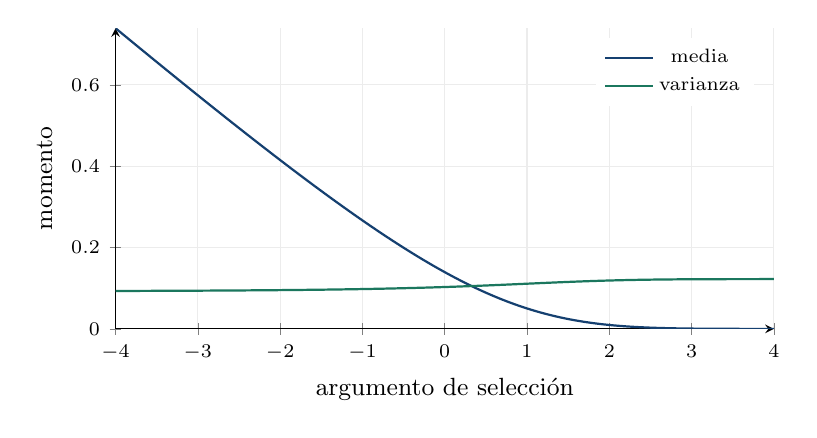
\begin{tikzpicture}\begin{axis}[base,width=.82\textwidth,height=5.4cm,xlabel={argumento de selección},ylabel={momento},legend pos=north east]
\addplot[azul,thick] coordinates {(-4,0.7394813) (-3.95,0.7311436) (-3.9,0.7228139) (-3.85,0.7144925) (-3.8,0.7061796) (-3.75,0.6978754) (-3.7,0.6895801) (-3.65,0.681294) (-3.6,0.6730173) (-3.55,0.6647504) (-3.5,0.6564935) (-3.45,0.6482468) (-3.4,0.6400108) (-3.35,0.6317856) (-3.3,0.6235716) (-3.25,0.6153692) (-3.2,0.6071786) (-3.15,0.5990002) (-3.1,0.5908345) (-3.05,0.5826817) (-3,0.5745423) (-2.95,0.5664166) (-2.9,0.5583051) (-2.85,0.5502083) (-2.8,0.5421266) (-2.75,0.5340604) (-2.7,0.5260102) (-2.65,0.5179766) (-2.6,0.50996) (-2.55,0.5019611) (-2.5,0.4939803) (-2.45,0.4860183) (-2.4,0.4780757) (-2.35,0.4701531) (-2.3,0.4622511) (-2.25,0.4543704) (-2.2,0.4465118) (-2.15,0.438676) (-2.1,0.4308636) (-2.05,0.4230756) (-2,0.4153127) (-1.95,0.4075758) (-1.9,0.3998657) (-1.85,0.3921834) (-1.8,0.3845298) (-1.75,0.3769059) (-1.7,0.3693126) (-1.65,0.3617512) (-1.6,0.3542226) (-1.55,0.346728) (-1.5,0.3392685) (-1.45,0.3318454) (-1.4,0.32446) (-1.35,0.3171135) (-1.3,0.3098074) (-1.25,0.3025429) (-1.2,0.2953216) (-1.15,0.288145) (-1.1,0.2810145) (-1.05,0.2739319) (-1,0.2668987) (-0.95,0.2599166) (-0.9,0.2529875) (-0.85,0.2461132) (-0.8,0.2392954) (-0.75,0.2325361) (-0.7,0.2258374) (-0.65,0.2192011) (-0.6,0.2126295) (-0.55,0.2061246) (-0.5,0.1996886) (-0.45,0.1933238) (-0.4,0.1870323) (-0.35,0.1808166) (-0.3,0.174679) (-0.25,0.1686219) (-0.2,0.1626478) (-0.15,0.156759) (-0.1,0.1509581) (-0.05,0.1452475) (0,0.1396298) (0.05,0.1341075) (0.1,0.1286831) (0.15,0.123359) (0.2,0.1181378) (0.25,0.1130219) (0.3,0.1080136) (0.35,0.1031154) (0.4,0.09832947) (0.45,0.09365799) (0.5,0.08910308) (0.55,0.08466671) (0.6,0.08035075) (0.65,0.07615693) (0.7,0.07208683) (0.75,0.06814186) (0.8,0.06432325) (0.85,0.06063204) (0.9,0.05706906) (0.95,0.05363492) (1,0.05032999) (1.05,0.04715443) (1.1,0.0441081) (1.15,0.04119064) (1.2,0.0384014) (1.25,0.03573946) (1.3,0.03320363) (1.35,0.03079246) (1.4,0.02850421) (1.45,0.02633688) (1.5,0.02428821) (1.55,0.02235568) (1.6,0.02053653) (1.65,0.0188278) (1.7,0.01722629) (1.75,0.01572861) (1.8,0.0143312) (1.85,0.01303037) (1.9,0.01182226) (1.95,0.01070294) (2,0.009668376) (2.05,0.008714481) (2.1,0.007837135) (2.15,0.007032209) (2.2,0.006295584) (2.25,0.005623179) (2.3,0.00501097) (2.35,0.004455006) (2.4,0.003951435) (2.45,0.003496512) (2.5,0.003086619) (2.55,0.002718277) (2.6,0.002388151) (2.65,0.002093066) (2.7,0.001830008) (2.75,0.00159613) (2.8,0.001388752) (2.85,0.001205369) (2.9,0.00104364) (2.95,0.0009013944) (3,0.0007766218) (3.05,0.0006674721) (3.1,0.000572247) (3.15,0.0004893947) (3.2,0.0004175023) (3.25,0.0003552884) (3.3,0.0003015954) (3.35,0.0002553811) (3.4,0.000215711) (3.45,0.0001817502) (3.5,0.000152755) (3.55,0.0001280659) (3.6,0.0001070999) (3.65,8.934309e-05) (3.7,7.434456e-05) (3.75,6.17097e-05) (3.8,5.109441e-05) (3.85,4.219964e-05) (3.9,3.476638e-05) (3.95,2.857099e-05) (4,2.342103e-05)};\addlegendentry{media}
\addplot[verde,thick] coordinates {(-4,0.09330436) (-3.95,0.09333207) (-3.9,0.09336053) (-3.85,0.09338977) (-3.8,0.09341981) (-3.75,0.09345069) (-3.7,0.09348243) (-3.65,0.09351505) (-3.6,0.09354859) (-3.55,0.09358309) (-3.5,0.09361857) (-3.45,0.09365507) (-3.4,0.09369263) (-3.35,0.09373128) (-3.3,0.09377106) (-3.25,0.09381201) (-3.2,0.09385418) (-3.15,0.0938976) (-3.1,0.09394233) (-3.05,0.0939884) (-3,0.09403588) (-2.95,0.0940848) (-2.9,0.09413522) (-2.85,0.09418721) (-2.8,0.0942408) (-2.75,0.09429608) (-2.7,0.09435309) (-2.65,0.0944119) (-2.6,0.09447258) (-2.55,0.09453519) (-2.5,0.09459982) (-2.45,0.09466654) (-2.4,0.09473541) (-2.35,0.09480654) (-2.3,0.09487999) (-2.25,0.09495586) (-2.2,0.09503424) (-2.15,0.09511523) (-2.1,0.09519891) (-2.05,0.0952854) (-2,0.0953748) (-1.95,0.09546721) (-1.9,0.09556276) (-1.85,0.09566156) (-1.8,0.09576373) (-1.75,0.09586939) (-1.7,0.09597869) (-1.65,0.09609174) (-1.6,0.09620869) (-1.55,0.09632968) (-1.5,0.09645486) (-1.45,0.09658439) (-1.4,0.0967184) (-1.35,0.09685708) (-1.3,0.09700057) (-1.25,0.09714905) (-1.2,0.09730269) (-1.15,0.09746166) (-1.1,0.09762614) (-1.05,0.09779631) (-1,0.09797237) (-0.95,0.09815448) (-0.9,0.09834284) (-0.85,0.09853764) (-0.8,0.09873907) (-0.75,0.09894731) (-0.7,0.09916256) (-0.65,0.09938499) (-0.6,0.09961479) (-0.55,0.09985214) (-0.5,0.1000972) (-0.45,0.1003502) (-0.4,0.1006112) (-0.35,0.1008804) (-0.3,0.1011579) (-0.25,0.1014438) (-0.2,0.1017384) (-0.15,0.1020415) (-0.1,0.1023534) (-0.05,0.1026741) (0,0.1030035) (0.05,0.1033417) (0.1,0.1036887) (0.15,0.1040444) (0.2,0.1044086) (0.25,0.1047813) (0.3,0.1051623) (0.35,0.1055514) (0.4,0.1059483) (0.45,0.1063526) (0.5,0.1067641) (0.55,0.1071824) (0.6,0.1076069) (0.65,0.1080373) (0.7,0.1084729) (0.75,0.1089131) (0.8,0.1093573) (0.85,0.1098047) (0.9,0.1102547) (0.95,0.1107065) (1,0.1111591) (1.05,0.1116118) (1.1,0.1120637) (1.15,0.1125137) (1.2,0.112961) (1.25,0.1134047) (1.3,0.1138437) (1.35,0.1142771) (1.4,0.114704) (1.45,0.1151234) (1.5,0.1155344) (1.55,0.1159362) (1.6,0.116328) (1.65,0.116709) (1.7,0.1170784) (1.75,0.1174357) (1.8,0.1177803) (1.85,0.1181116) (1.9,0.1184293) (1.95,0.1187331) (2,0.1190226) (2.05,0.1192977) (2.1,0.1195584) (2.15,0.1198047) (2.2,0.1200366) (2.25,0.1202543) (2.3,0.120458) (2.35,0.120648) (2.4,0.1208248) (2.45,0.1209886) (2.5,0.1211401) (2.55,0.1212796) (2.6,0.1214077) (2.65,0.121525) (2.7,0.121632) (2.75,0.1217293) (2.8,0.1218176) (2.85,0.1218974) (2.9,0.1219693) (2.95,0.1220338) (3,0.1220917) (3.05,0.1221433) (3.1,0.1221892) (3.15,0.12223) (3.2,0.122266) (3.25,0.1222978) (3.3,0.1223257) (3.35,0.1223502) (3.4,0.1223716) (3.45,0.1223902) (3.5,0.1224064) (3.55,0.1224204) (3.6,0.1224325) (3.65,0.1224429) (3.7,0.1224519) (3.75,0.1224595) (3.8,0.122466) (3.85,0.1224716) (3.9,0.1224763) (3.95,0.1224802) (4,0.1224836)};\addlegendentry{varianza}
\end{axis}\end{tikzpicture}\caption{Media y varianza del error salarial seleccionado con escala .35 y correlación .5.}\end{figure}

El argumento representa todos los regresores y efectos temporales de la selección sumados. Un argumento bajo impone un umbral exigente y selecciona errores de participación altos.

La media salarial seleccionada se desplaza según la correlación. La varianza salarial seleccionada combina la varianza truncada de $\nu_i$ y la parte independiente del error salarial. Ambas curvas se calculan con las integrales desarrolladas, no con imágenes externas.

\clearpage
\section{Figura del perfil de experiencia y de la diferencia exacta de un año}
\begin{figure}[H]\centering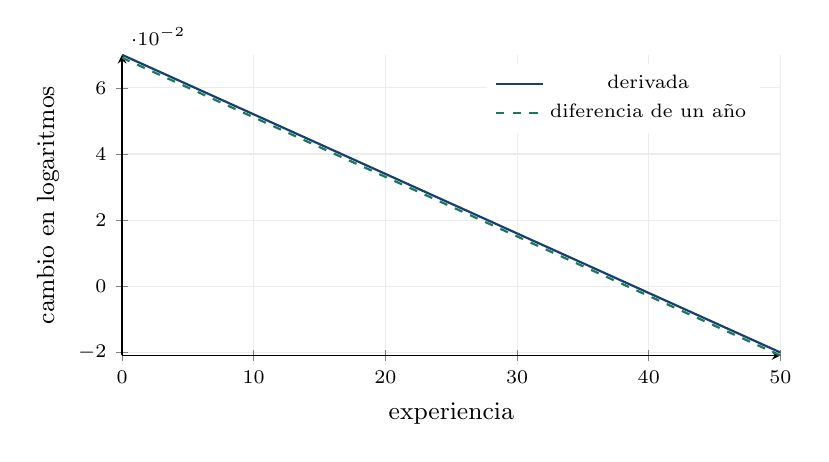
\begin{tikzpicture}\begin{axis}[base,width=.82\textwidth,height=5.4cm,xlabel={experiencia},ylabel={cambio en logaritmos},legend pos=north east]
\addplot[azul,thick,domain=0:50]{.07-.0018*x};\addlegendentry{derivada}
\addplot[verde,dashed,thick,domain=0:50]{.07-.0009*(2*x+1)};\addlegendentry{diferencia de un año}
\end{axis}\end{tikzpicture}\caption{Pendiente continua y diferencia de un año para el perfil ilustrativo .07 y -.0009.}\end{figure}

La diferencia discreta es la pendiente evaluada en el punto intermedio $t+1/2$ para este polinomio cuadrático. Esa igualdad se comprueba sustituyendo $2(t+1/2)$ en la derivada.

Educación, controles productivos y calendario siguen presentes en la ecuación; se mantienen iguales en esta comparación. La figura muestra una contribución parcial, no una regresión simplificada que elimina esos controles.

\clearpage
\section{Por qué una esperanza finita del probit no se presume automáticamente}

Fijar un diseño de selección de rango completo no garantiza un máximo finito para todas las realizaciones binarias. Para parámetros finitos, cada probabilidad normal está estrictamente entre cero y uno.

El patrón $S_1=\cdots=S_n=1$ tiene probabilidad
\[
\prod_{i=1}^n\Phi(Z_i^{\mathsf T}\pi+\lambda_{y(i)}^{(S)}+\mu_{m(i)}^{(S)})>0.
\]
Si el diseño contiene intercepto, llevarlo hacia más infinito hace que la log-verosimilitud de ese patrón aumente hacia cero. No existe un intercepto finito que alcance ese supremo. El patrón de todos ceros produce el problema simétrico.

Por ello, el estimador probit ordinario no es una función finita definida en todo el espacio de muestras. No se puede escribir sin condiciones
$\E[\widehat\pi]=\pi$ ni una covarianza finita universal.

En la realización observada de este libro existe una raíz finita. Los resultados asintóticos se refieren a diseños y secuencias donde la probabilidad de separación se controla y la información límite es no singular.

Condicionar a patrones con máximo finito, definir un estimador restringido o usar otra regla de estimación produce un objeto estadístico distinto. Las esperanzas exactas de ese objeto se escriben con su regla y su espacio de definición, no con una afirmación de insesgadez heredada de MCO.

\clearpage
\section{Esperanza exacta de dos etapas como suma sobre patrones de selección}

Para un diseño fijo, una realización binaria es $s=(s_1,\ldots,s_n)$. Su probabilidad, con independencia entre personas, es
\[
\begin{aligned}
\Prob(S=s\mid Z)
=\prod_i&
\Phi(Z_i^{\mathsf T}\pi+\lambda_{y(i)}^{(S)}+\mu_{m(i)}^{(S)})^{s_i}\\
&\cdot\Phi(-Z_i^{\mathsf T}\pi-\lambda_{y(i)}^{(S)}-\mu_{m(i)}^{(S)})^{1-s_i}.
\end{aligned}
\]
Sea $\mathcal S$ el conjunto de patrones donde el probit tiene raíz finita y el diseño salarial ampliado es de rango completo. La razón estimada para un diseño fijo es una función del patrón $s$; el probit no usa los salarios.

Al fijar ese patrón, la segunda etapa sigue siendo lineal en los salarios observados. Su esperanza se obtiene multiplicando su matriz de pesos por las medias seleccionadas verdaderas:
\[
W_i^{\mathsf T}\beta+
\kappa\frac{\phi(Z_i^{\mathsf T}\pi+\lambda_{y(i)}^{(S)}+\mu_{m(i)}^{(S)})}
{\Phi(Z_i^{\mathsf T}\pi+\lambda_{y(i)}^{(S)}+\mu_{m(i)}^{(S)})}.
\]
La razón de esos parámetros verdaderos no es necesariamente la razón estimada para el patrón. De ahí que no se deduzca insesgadez exacta de dos etapas.

La esperanza condicional a existencia se calcula como
\[
\sum_{s\in\mathcal S}
\frac{\Prob(S=s\mid Z)}{\Prob(S\in\mathcal S\mid Z)}
\E[(\widehat\beta^{\mathsf T},\widehat\kappa)^{\mathsf T}\mid W,Z,S=s].
\]
Es una suma exacta de hasta $2^n$ patrones; la aproximación asintótica permite evitar esa enumeración cuando sus condiciones se cumplen.

\clearpage
\section{Covarianza exacta por patrones y la diferencia con el sándwich asintótico}

El vector estimado de dos etapas, condicionado a existencia, admite la descomposición de covarianza total:
\[
\begin{aligned}
\Cov\left[\begin{pmatrix}\widehat\beta\\\widehat\kappa\end{pmatrix}
\Bigm|W,Z,S\in\mathcal S\right]
={}&
\E\left[
\Cov\left(\begin{pmatrix}\widehat\beta\\\widehat\kappa\end{pmatrix}
\Bigm|W,Z,S\right)\Bigm|S\in\mathcal S\right]\\
&+\Cov\left[
\E\left(\begin{pmatrix}\widehat\beta\\\widehat\kappa\end{pmatrix}
\Bigm|W,Z,S\right)\Bigm|S\in\mathcal S\right].
\end{aligned}
\]
El primer término promedia covarianzas de salarios seleccionados para matrices de pesos fijadas por cada patrón. El segundo mide cómo cambian esas medias estimadas entre patrones. Se evalúan con las probabilidades de la unidad anterior.

La primera etapa aporta además la aleatoriedad de sus coeficientes a través del patrón. La covarianza conjunta con ellos sigue la misma descomposición, incluyendo los cruces entre medias de parámetros.

Para máxima verosimilitud conjunta, la raíz es además una función no lineal de salarios. Sus momentos exactos requieren integrar esa función con la densidad conjunta seleccionada desarrollada antes, sobre su espacio de existencia.

La inversa de la Hessiana y el sándwich de momentos son covarianzas de primer orden bajo regularidad. No reemplazan estas sumas e integrales como identidades finitas exactas. La distinción explica por qué se pueden deducir todos los componentes sin afirmar una fórmula cerrada que el estimador no posee.

\clearpage
\section{Fuentes primarias y relación exacta con el documento suministrado}

La fuente de especificación es el archivo de tesis suministrado y el texto del apartado 7.3 enviado en esta conversación. Se conservaron sus ecuaciones de referencia, principal y selección. El documento no incluye una lista cerrada de $Z_i$ ni los microdatos para reestimar.

El desarrollo explica la diferencia entre $A_i$ y $\widetilde A_i$ que aparece entre la ecuación principal escrita y su interpretación. No añade Internet general o laboral como regresores de esa ecuación. Esas medidas permanecen como complementarias, según el texto de la tesis.

Las referencias siguientes fundamentan los temas; las operaciones algebraicas, integrales y laboratorios se desarrollan en el propio documento.
\begin{thebibliography}{9}
\bibitem{tesis} Ilizarbe Gonzales, E. M. Tesis suministrada: \emph{TIC y mercado laboral: mejores ingresos para trabajadores formales e informales en Lima Metropolitana y Callao}. Secciones Variables y Metodología, ecuaciones (8)--(10), más el apartado 7.3 proporcionado por el autor.
\bibitem{mincer1974} Mincer, J. (1974). \emph{Schooling, Experience, and Earnings}. National Bureau of Economic Research.
\url{https://www.nber.org/books-and-chapters/schooling-experience-and-earnings}
\bibitem{heckman1979} Heckman, J. J. (1979). Sample Selection Bias as a Specification Error. \emph{Econometrica}, 47(1), 153--161. DOI: 10.2307/1912352.
\url{https://www.jstor.org/stable/1912352}
\bibitem{hansen2022} Hansen, B. E. (2022). \emph{Econometrics}. Princeton University Press.
\url{https://users.ssc.wisc.edu/~behansen/econometrics/}
\bibitem{stataheckman} StataCorp. \emph{Heckman selection model}. Manual oficial del comando y sus métodos.
\url{https://www.stata.com/manuals/rheckman.pdf}
\end{thebibliography}

\end{document}
